\documentclass[11pt,a4paper]{extbook}

\usepackage[protrusion=true,expansion=true]{microtype}

%\usepackage[center]{titlesec}

\usepackage[pdftex,
            pdfauthor={Sanath Devalapurkar},
	    pdftitle={Algebraic topology}]{hyperref}
\usepackage{sseqpages}

\usepackage{listings}

\usepackage[T1]{fontenc}

%\usepackage[urw-garamond]{mathdesign}
\usepackage[left=2in,right=2in,top=2in,bottom=2.5in]{geometry}

\usepackage{todonotes}

\usepackage{amsmath}
%\usepackage{amsfonts}
\usepackage{amssymb}
\usepackage{float}
\usepackage{amsthm}
\usepackage{comment}
%\usepackage{amscd}

%\usepackage{txfonts} % Thanks to Eric for showing me that this font exists.
\usepackage{kpfonts}

\usepackage{color}
\usepackage[all]{xy}
\usepackage{verbatim}
\usepackage{setspace}
\usepackage[mathscr]{eucal}
\usepackage{graphicx}
\usepackage{tikz-cd}

\theoremstyle{theorem}
\newtheorem{theorem}{Theorem}[section]
\newtheorem{prop}[theorem]{Proposition}
\newtheorem{lemma}[theorem]{Lemma}
\newtheorem{corollary}[theorem]{Corollary}

\theoremstyle{definition}
\newtheorem{problem}[theorem]{Problem}
\newtheorem{definition}[theorem]{Definition}
\newtheorem{notation}[theorem]{Notation}
\newtheorem{summary}[theorem]{Summary}
\newtheorem{note}[theorem]{Note}
\newtheorem{claim}[theorem]{Claim}
\newtheorem{exercise}[theorem]{Exercise}
\newtheorem{construction}[theorem]{Construction}
%\theoremstyle{remark}
\newtheorem{remark}[theorem]{Remark}
\newtheorem{example}[theorem]{Example}
\newtheorem{question}[theorem]{Question}
\newtheorem{slogan}[theorem]{Slogan}
\newtheorem{warning}[theorem]{Warning}

\DeclareMathOperator{\Th}{Th}
\DeclareMathOperator{\Aut}{Aut}
\DeclareMathOperator{\coeq}{coeq}
\DeclareMathOperator{\colim}{colim}
\DeclareMathOperator{\coker}{coker}
\DeclareMathOperator{\cone}{cone}
\DeclareMathOperator{\Der}{Der}
\DeclareMathOperator{\Ext}{Ext}
\DeclareMathOperator{\Fun}{Fun}
\DeclareMathOperator{\hocolim}{hocolim}
\DeclareMathOperator{\holim}{holim}
\DeclareMathOperator{\Hom}{Hom}
\DeclareMathOperator{\Iso}{Iso}
\DeclareMathOperator{\img}{im}
\DeclareMathOperator{\Map}{Map}
\DeclareMathOperator{\Tot}{Tot}
\DeclareMathOperator{\Tor}{Tor}
\DeclareMathOperator{\Res}{Res}
\DeclareMathOperator{\Spec}{Spec}
\DeclareMathOperator{\rank}{Rank}
\DeclareMathOperator{\Vect}{Vect}

\def\llarrow{  \hspace{.05cm}\mbox{\,\put(0,-2){$\leftarrow$}\put(0,2){$\leftarrow$}\hspace{.45cm}}}
\def\rrarrow{  \hspace{.05cm}\mbox{\,\put(0,-2){$\rightarrow$}\put(0,2){$\rightarrow$}\hspace{.45cm}}}
\def\lllarrow{ \hspace{.05cm}\mbox{\,\put(0,-3){$\leftarrow$}\put(0,1){$\leftarrow$}\put(0,5){$\leftarrow$}\hspace{.45cm}}}
\def\rrrarrow{ \hspace{.05cm}\mbox{\,\put(0,-3){$\rightarrow$}\put(0,1){$\rightarrow$}\put(0,5){$\rightarrow$}\hspace{.45cm}}}

\def\cA{\mathcal A}\def\cB{\mathcal B}
\def\cc{\mathcal C}\def\cC{\mathbf C}
\def\cd{\mathcal D}
\def\ce{\mathcal E}\def\cf{\mathcal F}\def\cG{\mathcal G}\def\cH{\mathcal H}
\def\cI{\mathcal I}\def\cJ{\mathcal J}\def\cK{\mathcal K}\def\cL{\mathcal L}
\def\cM{\mathcal M}\def\cN{\mathcal N}\def\cO{\mathbf O}\def\cP{\mathcal P}
\def\cQ{\mathcal Q}\def\cR{\mathcal R}\def\cS{\mathcal S}\def\cT{\mathcal T}
\def\cU{\mathcal U}\def\cV{\mathcal V}\def\cW{\mathcal W}\def\cX{\mathcal X}
\def\cY{\mathcal Y}\def\cZ{\mathcal Z}

\def\AA{\mathbb A}\def\BB{\mathbb B}\def\CC{\mathbf C}\def\DD{\mathbb D}
\def\EE{\mathbb E}\def\FF{\mathbf F}\def\GG{\mathbb G}\def\HH{\mathbb H}
\def\II{\mathbb I}\def\JJ{\mathbb J}\def\KK{\mathbb K}\def\LL{\mathbb L}
\def\MM{\mathcal M}\def\NN{\mathbb N}\def\OO{\mathbb O}\def\PP{\mathbf P}
\def\QQ{\mathbf Q}\def\RR{\mathbf R}\def\SS{\mathbb S}\def\TT{\mathbb T}
\def\UU{\mathbb U}\def\VV{\mathbb V}\def\WW{\mathbb W}\def\XX{\mathbb X}
\def\YY{\mathbb Y}\def\ZZ{\mathbf Z}

\usepackage{amsbsy}

\newcommand{\CP}{\mathbf{CP}}
\newcommand{\RP}{\mathbf{RP}}
\newcommand{\Set}{\mathrm{Set}}
\newcommand{\Gra}{\mathrm{Gr}}
\newcommand{\GL}{\mathrm{GL}}
\newcommand{\gl}{\mathit{gl}}

\newcommand{\nn}{\nonumber}
\newcommand{\nid}{\noindent}
\newcommand{\ra}{\rightarrow}
\newcommand{\la}{\leftarrow}
\newcommand{\xra}{\xrightarrow}
\newcommand{\xla}{\xleftarrow}

\newcommand{\weq}{\xrightarrow{\sim}}
\newcommand{\cofib}{\rightarrowtail}
\newcommand{\fib}{\twoheadrightarrow}
%\newcommand{\cofib}{\to}
%\newcommand{\fib}{\to}

\newcommand\cHH{\check{H}}
\newcommand{\Fl}{F\ell}
\newcommand{\Fr}{Fr}
\newcommand\cCC{\check{C}}
\newcommand{\MFGL}{\mathcal M_{\mathit{FGL}}}
\newcommand{\calO}{{\mathcal O}}
\newcommand{\calC}{{\mathcal C}}
\newcommand{\set}{{\mathrm{Set}}}
\newcommand{\Deltab}{{\Delta}} %change this to bold Delta. This is like this here because garamond fucks up bold things.
\newcommand{\spec}{\mathrm{Spec}}
\newcommand{\Z}{\mathbf Z}
\newcommand{\Sin}{\mathrm{Sin}}
\newcommand{\htop}{\mathrm{Ho}(\mathbf{Top})}
\newcommand{\sca}{\mathcal{A}}
\DeclareMathOperator{\Spf}{Spf}
\renewcommand{\Top}{\mathbf{Top}}
\newcommand{\CG}{\mathbf{CG}}
\newcommand{\Ab}{\mathbf{Ab}}
\newcommand{\Bun}{\mathrm{Bun}}
\newcommand{\Ho}{\mathrm{Ho}}
\newcommand{\gr}{\mathrm{gr}}
\newcommand{\sk}{\mathrm{sk}}
\newcommand{\Cat}{\mathbf{Cat}}
\newcommand{\xar}[1]{\xrightarrow{{#1}}}
\newcommand{\pr}{\mathrm{pr}}
%%%%%%%%%%%%%%%%

%\usepackage{ebgaramond}
%\usepackage{fancyhdr}
% 
%\newcommand{\myheader}{
%    \ifnum\value{section} > 38
%    18.906
%    \else
%    18.905
%    \fi
%}

%\pagestyle{fancy}
%\fancyhf{}
%\fancyhead[LE]{Notes by Sanath Devalapurkar}
%\fancyhead[LO]{Taught by Haynes Miller}
%\chead{Notes for \myheader}
%\rhead{Lecture \thesection}
%\cfoot{\thepage}


\begin{document}
\title{Algebraic Topology}
\author{Taught by Haynes Miller;\\
Notes by Sanath Devalapurkar;\\
Edited by Sanath Devalapurkar, John Ni, and others %add other folks who've contributed here
}
%\date{Fall 2016 -- Spring 2017}

\frontmatter

\maketitle
\cleardoublepage
\subsection*{Preface}
18.905/906 is being taught by Professor Haynes Miller in Fall 2016/Spring 2017 (respectively). I am planning on taking notes throughout the semester. I'll add drawings by putting them on a notepad, scanning them as images, and finally inserting them in the appropriate spots. This means that they might be messy. Any mistakes in these notes are only mine, and not Professor Miller's.

Here are hyperlinks to the notes from each of the semesters.
    \begin{enumerate}
        \item The notes for 18.905 start at section \ref{905}.
        \item The notes for 18.906 start at section \ref{906}.
    \end{enumerate}

\tableofcontents
\newpage

\mainmatter

% The current division of labor is: John'll "work on the first part (like, most of 905)",
% and skd will start off by editing/rewriting the whole of 906.

\part{18.905: an introduction to algebraic topology}\label{905}

\chapter{Homology and CW-complexes}
% I removed the definition of a manifold and moved it in-line for better flow.
% I think it's best to use /emph in definitions to show what's being defined.
% Put periods even in display math!
% For spacing reasons, should use \colon instead of : for functions, e.g. f \colon A \to B.
% Since ker is lowercase, im probably should be also.

\section{Introduction, simplices}\label{905}
In 18.905, which is the first half of this book, we will cover the following topics:
\begin{enumerate}
    \item Singular homology
    \item CW-complexes
    \item Basics of category theory
    \item Homological algebra
    \item The K\"{u}nneth theorem
    \item UCT, cohomology
    \item Cup and cap products, and
    \item Poincar\'{e} duality.
\end{enumerate}
Below are some examples of commonly encountered topological spaces.
\begin{itemize}
    \item The most basic is \emph{$n$-dimensional Euclidean space}, $\mathbf{R}^n$.
    \item The \emph{$n$-sphere} $S^n=\{x\in \mathbf{R}^{n+1}:|x|=1\}$ is topologized as a subspace of $\mathbf{R}^{n+1}$.
    \item Identifying antipodal points in $S^n$ gives \emph{real projective space} $\mathbf{RP}^n=S^n / (x\sim -x)$, i.e. the space of lines through the origin in $\mathbf{R}^{n+1}$.
    \item Call an ordered collection of $k$ orthonormal vectors an \emph{orthonormal $k$-frame}. The space of orthonormal $k$-frames in $\mathbf{R}^n$ forms the \emph{Stiefel manifold} $V_k(\mathbf{R}^n)$, which is topologized as a subspace of $(S^{n-1})^k$.
    \item Let $x\sim y$ if $x$ and $y$ are $k$-frames with the same span. The \emph{Grassmannian} is the quotient $\mathrm{Gr}_k(\mathbf{R}^n)=V_k(\mathbf{R}^n)/\sim$. In particular, $\mathbf{Gr}_1(\mathbf{R}^n) = \mathbf{RP}^{n-1}$.
\end{itemize}
The above are all \emph{manifolds}, which are Hausdorff spaces locally homeomorphic to Euclidean space. Aside from $\mathbf{R}^n$ itself, the preceding examples are also compact. Such spaces exhibit a hidden symmetry, which is the culmination of 18.905: Poincar\'{e} duality.

As the name suggests, the central aim of algebraic topology is the usage of algebraic tools to study topological spaces. A common technique is to probe topological spaces via maps to them. In different ways, this approach gives rise to singular homology and homotopy groups. We now detail the former; the latter takes stage in 18.906.
\begin{definition}
For $n\geq 0$, the \emph{standard $n$-simplex} $\Delta^n$ is the convex hull of the standard basis $\{e_0,\cdots,e_n\}$ in $\mathbf{R}^{n+1}$. More explicitly,
$$\Delta^n = \left\{\sum t_i e_i : \sum t_i = 1, t_i\geq 0\right\}\subseteq\mathbf{R}^{n+1}.$$
The $t_i$ are called barycentric coordinates.
\end{definition}
We will write $i$ in lieu of $e_i$ to refer to the vertices of $\Delta^n$. The standard simplicies are related by face inclusions $d^i\colon \Delta^{n-1} \to \Delta^{n}$ for $0\leq i \leq n$, where $d^i$ misses the vertex $i$. \todo{Insert pic here.}
\begin{definition}
Let $X$ be any topological space. A singular $n$-simplex in $X$ is a continuous map $\Delta^n\to X$. Denote by $\mathrm{Sin}_n(X)$ the set of all $n$-simplices in $X$.
    
    This seems like a rather bold construction to make, as $\mathrm{Sin}_n(X)$ is huge. Nonetheless, we will soon make it even larger.
\end{definition}
(See drawing for a torus\todo{Image me}. The direction of the simplex is like an orientation given by ordering of the indices of $\Delta^n$. The standard notation is $\sigma:\Delta^n\to X$.)\todo{Depict this whole thing as an image, and remove the sentence when done}

For $0\leq i \leq n$, precomposition by the face inclusion $d^i$ produces a map $d_i\colon \Sin_n(X)\to\Sin_{n-1}(X)$ sending $\sigma\mapsto\sigma\circ d^i$, which is the $i$th face of $\sigma$. This allows us to make sense of the ``boundary'' of a simplex, and we are particularly interested in simplices for which that boundary vanishes.

For example, if $\sigma$ is a 1-simplex that goes around the hole in a torus $T$, then $d_1\sigma = d_0\sigma$. To express that the boundary vanishes, we want to write $d_0\sigma - d_1\sigma=0$, but this difference is no longer a simplex. To accomodate such formal sums, we will enlarge $\mathrm{Sin}_n(X)$ further by considering the free abelian group it generates.
\begin{definition}
The abelian group $S_n(X)$ of \emph{singular $n$-chains} in $X$ is the free abelian group generated by $n$-simplices
$$S_n(X) = \mathbf{Z}\Sin_n(X).$$
    Its elements are finite linear combinations, i.e. formal sums $\sum_{i\in\text{finite set}}a_i\sigma_i$\todo{idk what was meant by ``display'' in the comments} where $a_i\in\mathbf{Z}$. If $n<0$, say that $S_n(X)=0$. Now, define
$$\partial\colon \Sin_n(X)\to S_{n-1}(X),$$
$$\partial\sigma = \sum_{i=0}^n(-1)^i d_i\sigma.$$
This extends to a homomorphism $\partial \colon S_n(X) \to S_{n-1}(X)$ by additivity.
\end{definition}
We use this homomorphism to obtain something more tractable than the entirety of $S_n(X)$. First we restrict our attention to chains with vanishing boundary.
\begin{definition}
An \emph{$n$-cycle} in $X$ is an $n$-chain $c$ with $\partial c = 0$. Denote $Z_n(X) = \ker(S_n(X)\xrightarrow{\partial}S_{n-1}(X))$.
\end{definition}
For example, with $\sigma$ on the torus described before, $\sigma\in Z_1(X)$ since $\partial \sigma = d_0\sigma - d_1\sigma = 0$.
\begin{theorem}
Any boundary is a cycle, i.e., $B_n(X) := \mathrm{Im}(\partial:S_{n+1}(X)\to S_n(X))\subseteq Z_n(X)$.
\end{theorem}
\begin{proof}
    Homework!
\end{proof}
With the preceding, we are prepared to define singular homology.
\begin{definition}
The $n$th singular homology group of $X$ is:
    $$ H_n(X) = Z_n(X)/B_n(X) = \frac{\ker(\partial:S_n(X)\to S_{n-1}(X))}{\mathrm{im}(\partial:S_{n+1}(X)\to S_n(X))}.$$
\end{definition}
Both $Z_n(X)$ and $B_n(X)$ are free abelian groups because they are subgroups of the free abelian group $S_n(X)$, but the quotient $H_n(X)$ isn't necessarily free. While $Z_n(X)$ and $B_n(X)$ are uncountably generated, $H_n(X)$ is finitely generated for the spaces we are interested in. If $T$ is the torus for example, then $H_1(T) \cong \mathbf{Z} \oplus \mathbf{Z}$ and $\sigma$ as described previously is one of the two generators.
\section{Simplices, more about homology}
Recall the standard $n$-simplex $\Delta^n\subseteq\mathbf{R}^{n+1}$. A singular simplex is a map $\sigma:\Delta^n\to X$; they are elements of the set $\Sin_n(X)$. For example, $\Sin_0(X)$ consists of points of $X$. You have a huge collection of maps $d^i:\Sin_n(X)\to\Sin_{n-1}(X)$ and $s^i:\Sin_n(X)\to\Sin_{n+1}(X)$, and the collection $\{\Sin_n(X),d^i,s^i\}$ forms a simplicial set. You therefore get a functor $\mathbf{Top}\to\{\text{simplicial sets}\}$. Simplicial sets are really cool, because they're combinatorial models for topological spaces.

Now, you get induced maps on free abelian groups. This produces for each space a semi-simplicial abelian group. Using the $d^i$s and $s^i$s, you get a boundary map $\partial$, and therefore a chain complex because $\partial^2=0$ (see homework). We capture this process in a diagram:
\begin{equation*}
\xymatrix{\mathbf{Top}\ar[d]\ar[r] & \{\text{semi-simplicial sets}\}\ar[r] & \{\text{semi-simplicial abelian groups}\}\ar[d]\\
    \{\text{simplicial sets}\}\ar[ur] & & \{\text{chain complexes}\}\ar[d]^{\text{take homology}}\\
 & &\{\text{graded abelian group}\}}
\end{equation*}
If you have a chain complex $\partial:A_n\to A_{n-1}$, then you have its homology $H_n(A,\partial)=\ker\partial_n/\img\partial_n$.

Let's practice with simplices. Suppose we have $\sigma:\Delta^1\to X$. Construct a map $\phi:\Delta^1\to\Delta^1$ via $(t,1-t)\mapsto (1-t,t)$. This reverses the orientation of $\sigma$. Composing $\sigma$ with $\phi$ gives another singular simplex $\overline{\sigma}$. It is \textit{not} true that $\overline{\sigma}=-\sigma$ in $S_1(X)$.

Claim: $\overline{\sigma}\equiv -\sigma\bmod B_1(X)=\img(\partial)$, i.e., they are homologous. That is, if $d_0\sigma=d_1\sigma$, so $\sigma\in Z_1(X)$, then $[\overline{\sigma}]=-[\sigma]$ in $ H_1(X)$. In other words, $\overline{\sigma}+\sigma$ is a boundary. We have to come up with a $2$-simplex in $X$ whose boundary is $\overline{\sigma}+\sigma$.

Let $\pi$ denote the projection map from $[0,1,2]$ to $[0,1]$\todo{MUST UPLOAD PICTURE HERE}. Then, $\partial(\sigma\circ\pi)=\sigma\pi d^0-\sigma\pi d^1 +\sigma\pi d^2=\overline{\sigma}-c^1_{\sigma(0)}+\sigma$ where $c^1_{\sigma(0)}$ is the constant $1$-simplex at $\sigma(0)$ (similarly for $c^n_{\sigma(0)}$). The $c^1_{\sigma(0)}$ is an error term. How do we correct this? Consider the constant $2$-simplex $c^2_{\sigma(0)}$ at $\sigma(0)$; then the boundary is $c^1_{\sigma(0)}-c^1_{\sigma(0)}+c^1_{\sigma(0)}$, which is $c^1_{\sigma(0)}$. So, $\overline{\sigma}+\sigma=\partial(\sigma\circ\pi + c^2_{\sigma(0)})$.

Let's compute the homologies of $\emptyset$ and $\ast$. Well, $\Sin_n(\emptyset)=\emptyset$, so $S_\ast(\emptyset)=0$. So, $\cdots\to S_2\to S_1\to S_0$ is the zero chain complex. This means that $Z_\ast(\emptyset)=0$ and similarly for boundaries. The homology in all dimensions is therefore $0$.

Now for $\ast$. Clearly $\Sin_n(\ast)=\ast$, and this generates $S_n(\ast)$, which is thus $\mathbf{Z}$. The chain complex is $S_0(\ast)\leftarrow S_1(\ast)\leftarrow S_2(\ast)\leftarrow\cdots$. What are the boundary maps? Well, $\partial(c^1_\ast)=d^0c^1_\ast - d^1c^1_\ast = c^0_\ast - c^0_\ast = 0$, $\partial(c^2_\ast)=d^0c_2^\ast - d^1 c^2_\ast + d^2 c^2_\ast = c^1_\ast - c^1_\ast + c^1_\ast = c^1_\ast$, and $\partial (c^3_\ast)=d^0 c^3_\ast - d^1 c^3_\ast + d^2 c^3_\ast - d^3 c^3_\ast = 0$. This means that our chain complex is:
$$\cdots\to\mathbf{Z}\xrightarrow{0}\mathbf{Z}\xrightarrow{1}\mathbf{Z}\xrightarrow{0}\mathbf{Z}$$
The cycles therefore alternate between $0$s and $\mathbf{Z}$s, namely as $\mathbf{Z},\mathbf{Z},0,\mathbf{Z},0,\cdots$. The boundaries are the same as the cycles except for dimension zero, namely as $0,\mathbf{Z},0,\mathbf{Z},0,\cdots$. This means that $ H_0(\ast)=\mathbf{Z}$ but $ H_i(\ast)=0$ for $i>0$.

What do these constructions do? Suppose you have $f:X\to Y$. You have a map $f_\ast:\Sin_n(X)\to\Sin_n(Y)$ induced by composition, namely $\sigma\mapsto f\circ \sigma=:f_\ast\sigma$. What about face maps; does the following diagram commute?
\begin{eqnarray*}
\xymatrix{\Sin_n(X)\ar[r]^{f_\ast}\ar[d]^{d_i} & \Sin_n(Y)\ar[d]^{d_i}\\
\Sin_{n-1}(X)\ar[r]^{f_\ast} & \Sin_{n-1}(Y)}
\end{eqnarray*}
We see that $d_if_\ast\sigma=(f_\ast\sigma)\circ d^i=f\circ\sigma\circ d^i$, and $f_\ast(d_i\sigma)=f_\ast(\sigma\circ d^i)=f\circ\sigma\circ d^i$. So the answer is yes! This also holds for the free abelian groups. You therefore get a map of chain complexes.

A chain map $f:C_\ast\to D_\ast$ is a map $f_n:C_n\to D_n$ such that the following diagram commutes for every $n$:
\begin{equation*}
    \xymatrix{
	C_n\ar[r]^{f_n}\ar[d]^{partial_C} & D_n\ar[d]^{\partial_D}\\
	C_{n-1}\ar[r]^{f_{n-1}} & D_{n-1}
    }
\end{equation*}
Does a chain map induce a map in homology $f_\ast: H_n(C)\to H_n(D)$? As a preliminary question, do we get a map $Z_n(C)\to Z_n(D)$? Let $c\in Z_n(C)$, so that $\partial_C c = 0$. Then $\partial_D f_n(c) = f_{n-1}\partial_C c = f_{n-1}(0) = 0$, because $f$ is a chain map. This means that $f_n(c)$ is also an $n$-cycle, i.e., $f$ gives a map $Z_n(C)\to Z_n(D)$.

Do we also get a map $B_n(C)\to B_n(D)$? Let $c\in B_n(C)$, so that there exists $c^\prime \in C_{n+1}$ such that $\partial_C c^\prime = c$. Then $f_n(c) = f_n\partial_C c^\prime = \partial_D f_{n+1}(c^\prime)$. Thus $f_n(c)$ is the boundary of $f_{n+1}(c^\prime)$, and $f$ gives a map $B_n(C)\to B_n(D)$.

The two maps $Z_n(C)\to Z_n(D)$ and $B_n(C)\to B_n(D)$ give a map on homology. This means that we get a map $f_\ast: H_n(X)\to H_n(Y)$, as desired!


\section{Categories, functors, natural transformations}\label{categories}
Office hours. Hood Chatham's are Mondays, 1:30 - 3:30, in 2-390A. Miller's is Tuesdays, 3:00-5:00 in 2-478.

The collection of all topological spaces forms a category. Similarly with simplicial sets, denoted $\set_\Deltab$ or $s\set$. You can take $X\mapsto \Sin_\bullet(X)$, and if $X\to Y$ is a map of spaces, this induces $\Sin_\bullet(X)\to\Sin_\bullet(Y)$. This is a functor $\mathbf{Top}\to s\set$.
\begin{definition}
A category $\cc$ is a class $\mathrm{ob}(\cc)$ of objects, such that for every two objects, $\cc(X,Y)$ is a set (thought of as a set of maps from $X$ to $Y$); these are called morphisms. These satisfy the properties that for all $X\in\mathrm{ob}(\cc)$, there exists an element $1_X\in\cc(X,X)$ that acts as the identity, and for all $X,Y,X\in\mathrm{ob}(\cc)$, there is a composition $\cc(X,Y)\times\cc(Y,Z)\to\cc(X,Z)$. These in turn satisfy the following properties:
\begin{itemize}
\item $1_Y\circ f=f$, and $f\circ 1_X=f$.
\item Composition is associative.
\end{itemize}
\end{definition}
\begin{example}
The category of sets and functions between sets forms a category. The category of abelian groups and homomorphisms forms a category. Of course, topological spaces and continuous maps. A monoid, which is a category with one object. The simplex category (note that $|[n]|=n+1$). A poset forms a category; but note that if $x\leq y$ and $y\leq x$, then $x\cong y$, not $x=y$. The latter property holds if the only isomorphisms are identities.
\end{example}
A small category is one such that $\mathrm{ob}(\cc)$ is a set, not necessarily a class.
\begin{definition}
Let $\cc,\cd$ be categories. A functor $F:\cc\to\cd$ is a function $\mathrm{ob}(\cc)\to\mathrm{ob}(\cd)$, such that for all $x,y\in\mathrm{ob}(\cc)$, there is a map $\cc(x,y)\to\cc(F(x),F(y))$ that respects composition and the identity.

Let $F,G:\cc\to\cd$. A natural transformation $\theta:F\to G$ is a map $\theta(X):F(X)\to G(X)$ for all $X\in\mathrm{ob}(\cc)$, and a commuting diagram for all $f:X\to Y$:
\begin{equation*}
\xymatrix{F(X)\ar[d]^{F(f)}\ar[r]^{\theta(X)} & G(X)\ar[d]^{G(f)}\\
F(Y)\ar[r]^{\theta(Y)} & G(Y)}
\end{equation*}
\end{definition}
\begin{example}
The boundary map $\partial:S_n\to S_{n-1}$ is a natural transformation. Let $G$ be a group viewed as a one-point category. Any element $F\in\mathrm{Fun}(G,\mathbf{Ab})$ is simply a group action of $G$ on $F(\ast)=A$, i.e., a representation of $G$ in abelian groups. A natural transformation from $F\to F^\prime$ is just a $G$-equivariant map.
\end{example}

\section{More about categories, and computing the homology of a star-shaped region}
Let $\mathrm{Vect}_{\mathbf{C}}$ be the category of vector spaces and linear transformations. Given a $\mathbf{C}$-vector space $V$, you can consider the dual $V^\ast=\Hom(V,\cc)$. Is this a functor? If you have a linear transformation $F:V\to W$, you get a map $F^\ast:W^\ast\to V^\ast$, so this is like a functor, but isn't strictly functor. This preserves composition and identities. Taking the dual therefore gives a functor $\mathrm{Vect}_\cc^{op}\to\mathrm{Vect}_\cc$, which is a \textit{contravariant} functor.
\begin{definition}
Given $\cc,\cd$. A contravariant functor is a functor from $\cc^{op}\to\cd$ where $\cc^{op}$ has the same objects as the category $\cc$ but with all morphisms reversed. There's a contravariant functor $\cc\to\cc^{op}$ that is the identity on objects and on morphisms.
\end{definition}
Let $\cc$ be a category, and let $Y\in\mathrm{ob}(\cc)$. We get a map $\cc^{op}\to\set$ that takes $X\mapsto \cc(X,Y)$, and takes a map $X\to W$ to the map defined by composition $\cc(W,Y)\to \cc(X,Y)$. This is called the functor that is represented by $Y$. It is very important to note that $\cc(-,Y)$ is contravariant, but $\cc(Y,-)$ is covariant.

Recall that $\Deltab$ has objects $[0],[1],[2],\cdots$ and a functor $\Deltab\to\mathbf{Top}$ that sends $[n]\mapsto\Delta^n$. We get a map $\mathbf{Top}^{op}\to\set$ given by sending $X\mapsto\mathbf{Top}(\Delta^n,X)=:\Sin_n(X)$. The composition gives you a contravariant functor $\Delta^{op}\to\set$, which sends $[n]\mapsto\mathbf{Top}(\Delta^n,X)$. This, along with the description of what happens to the face and degeneracy maps (see psets!) is precisely the singular simplicial set of $X$. In other words:
\begin{prop}[Really a definition...]
Simplicial sets are precisely functors $\Deltab^{op}\to\set$, i.e., $s\set=\mathbf{Fun}(\Deltab^{op},\set)$. More generally, simplicial objects in a category $\cc$ are functors $\Deltab^{op}\to\cc$, i.e., $s\cc=\mathbf{Fun}(\Deltab^{op},\cc)$.
\end{prop}
(Note that $\mathbf{Fun}(\cc,\cd)$ is the category whose objects are functors and whose morphisms are natural transformations.) Semi-simplicial sets (only face maps, not necessarily degeneracy maps) in a category $\cc$ are simply $ss\cc=\mathbf{Fun}(\Deltab^{op}_{inj},\cc)$ where $\Deltab_{inj}$ consists of the objects of $\Deltab$ where the morphisms only consist of the injective maps.
\begin{definition}
Let $f:X\to Y$ be a morphism in a category $\cc$. Say that $f$ is a \textit{split epimorphism} if there exists $g:Y\to X$ (often called a section or a splitting) such that $Y\xrightarrow{g}X\xrightarrow{f}Y$ is the identity.
\end{definition}
\begin{example}
Let $\cc=\set$. If $f:X\to Y$ is a map of sets, then this says that for every element of $Y$, there exists some element of $X$ whose image in $Y$ is the original element. This means that $f$ is surjective. Is every surjective map a split epimorphism? This reduces to the axiom of choice because proving that if $y\in Y$, the map $g:Y\to X$ can be constructed by choosing some $x\in f^{-1}(y)$.
\end{example}
\begin{definition}
Say that $g:Y\to X$ is a split monomorphism if there is $f:X\to Y$ such that $f\circ g=1_Y$.
\end{definition}
\begin{example}
Let $\cc=\set$. Claim: it's an injection. If $y,y^\prime\in Y$, and $g(y)=g(y^\prime)$, we want to show that $y=y^\prime$. Apply $f$, to get $f(g(y))=y=f(g(y^\prime))=y^\prime$. If $Y\neq \emptyset$, then every injection $g:Y\to X$ is a split mono.
\end{example}
\begin{example}
An isomorphism is a split epi + split mono.
\end{example}
\begin{lemma}
If $f:X\to Y$ is a split epi or mono in $\cc$, and you have a functor $F:\cc\to \cd$, then so is $F(f)$ in $\cd$.
\end{lemma}
\begin{proof}
Trivial.
\end{proof}
\begin{example}
Suppose $\cc=\mathbf{Ab}$, and you have a split epi $f:A\to B$. We have a map $g:B\to A$ so that $fg=1$. Clearly $f$ must be surjective. Consider the kernel of $f$, so we have a composition $\ker f\to A\to B$. We also have a map $B\to A$, so we can add, and get $\ker f\oplus B\xrightarrow{[i,g]} A$ where $i$ is the inclusion $\ker f\to A$. Left for reader: $[i,g]$ is an isomorphism.

If $g:B\to A$ is a split mono, so there is $f:A\to B$ so that $fg=1$. Clearly $g$ is injective, and we get a map $B\to A\xrightarrow{p}\mathrm{coker}(g)$. We therefore get a map $A\xrightarrow{\begin{pmatrix}
p \\ f
\end{pmatrix}}\mathrm{coker}(g)\oplus B$. Left to reader again: this is an isomorphism.
\end{example}
We have to get into some topology, since it's on our agenda. Suppose I have a space $X$. There's always a unique map $X\to\ast$, which means categorically that $\ast$ is trivial. We have an induced map $ H_n(X)\to H_n(\ast)=\begin{cases}\mathbf{Z} & n=0\\
0 & \text{else}\end{cases}$. Consider the equivalence class (also called the \textit{homology class} of the cycle $\sum a_ix_i$) $\left[\sum a_ix_i\right]\in H_0(X)$, where $x_i$ is a point in $X$. Under the induced map, this goes as: $\left[\sum a_ix_i\right]\mapsto \left[\sum a_i\ast\right]=\left(\sum a_i\right)\left[\ast\right]$. This is called the augmentation map. This map is a split epi, because we can always choose a point of $X$ and pull an element of $\mathbf{Z}$ back. This motivates the following definition.
\begin{definition}
A pointed space is a pair $(X,\ast)$, with $\ast\in X$ called the \textit{basepoint}.
\end{definition}
We have an inclusion $\ast\to X\to\ast$, so we get an induced map $\mathbf{Z}\xrightarrow{\eta} H_\ast(X)\xrightarrow{\epsilon}\mathbf{Z}$, and the composition is the identity. The map $\epsilon$ is the augmentation map we described above. This means, by our above analysis, we see that $ H_\ast(X)\cong \mathbf{Z}\oplus\mathrm{coker}\eta \cong\mathbf{Z}\oplus\ker\epsilon$. The homology $ H_\ast(X,\ast)=\mathrm{coker}\eta$, and this is called the reduced homology of $(X,\ast)$. It's isomorphic to $ H_\ast(X)$ in dimensions greater than $0$, but differs by a factor of $\mathbf{Z}$ in dimension $0$.

We spent up a lot of time on categories, and didn't get to star-shaped regions. We'll pick this up on Friday, but we'll begin a little here.
\begin{definition}
A star-shaped region is a subspace $X$ of $\mathbf{R}^n$ for some $n$ such that $0\in X$, such that for all $x\in X$, and for all $t\in[0,1]$, $tx\in X$. 
\end{definition}
\begin{example}
Any convex region containing the origin is star shaped.
\end{example}
\begin{theorem}
The augmentation map $\epsilon: H_\ast(X)\to \mathbf{Z}$ is an isomorphism, i.e., $ H_0(X)\cong\mathbf{Z}$ and $ H_i(X)\cong 0$ for $i>0$.
\end{theorem}
The strategy of proof is that $\epsilon$ is induced by sending $X\to \ast$. We'll look at the chain map $S_\ast(x)\to\mathbf{Z}\to S_\ast(X)$. We'll show that this composite induces the same map in homology as the identity map, which means that the identity map factors through $\mathbf{Z}$, so we're done.


\section{Homotopy, star-shaped regions}
The idea of homotopy is the central concept of all of algebraic topology, to put it bluntly. We have a functor $ H_\ast:\mathbf{Top}\to\mathbf{Ab}$, but it's too crude to distinguish between topological spaces. The virtue of this definition is that it's computable, although it can't completely distinguish between two spaces.
\begin{definition}
Let $f_0,f_1:X\to Y$ be two maps. A homotopy from $f_0$ to $f_1$ is a map $h:X\times I\to Y$ such that $h(x,0)=f_0(x)$ and $f(x,1)=f_1(x)$. We say that $f_0$ and $f_1$ are homotopic, and this is written $f_0\sim f_1$ because this is an equivalence relation on maps (transitivity follows from the gluing lemma).
\end{definition}
We denote by $[X,Y]$ the set $\mathbf{Top}(X,Y)/\sim$. On Monday, we'll prove the following result.
\begin{theorem}
If $f_0\sim f_1$, then $ H_\ast(f_0)= H_\ast(f_1)$. In other words, homology cannot distinguish between homotopic things.
\end{theorem}
Suppose I have two maps $f_0,f_1:X\to Y$ and a map $g:Y\to Z$, with a homotopy $h:f_0\sim f_1$. Composing $h$ with $g$ gives a homotopy between $g\circ f_0$ and $g\circ f_1$. Precomposing also works. Namely, if $g:W\to X$ is a map and $f_0,f_1:X\to Y$ are homotopic, then $f_0g\sim f_1g$. Does this let us compose homotopy classes? That is, can we complete:
\begin{equation*}
\xymatrix{\mathbf{Top}(Y,Z)\times\mathbf{Top}(X,Y)\ar[d]\ar[r] & \mathbf{Top}(X,Z)\ar[d]\\
[Y,Z]\times[X,Y]\ar@{-->}[r] & [X,Z]}
\end{equation*}
The answer is yes. If $g_0\sim g_1:Y\to Z$ and $f_0\sim f_1: X\to Y$, then $g_0f_0\sim g_0f_1$, but this is just homotopic to $g_1f_1$. This therefore gives us a new category, called the homotopy category.
\begin{definition}
The homotopy category of topological spaces is $\mathrm{Ho}(\mathbf{Top})$ whose objects are topological spaces and $\mathrm{Ho}(\mathbf{Top})(X,Y)=[X,Y]=\mathbf{Top}(X,Y)/\sim$.
\end{definition}
This is an interesting category because it has \textit{terrible} categorical properties. The theorem that we'll prove on Monday says that the homology functor $ H_\ast:\mathbf{Top}\to\mathbf{Ab}$ factors as $\mathbf{Top}\to\mathrm{Ho}(\mathbf{Top})\to\mathbf{Ab}$.
\begin{definition}
A map $f:X\to Y$ is a homotopy equivalence if $[f]\in[X,Y]$ is an isomorphism in $\htop$. In other words, there is $g:Y\to X$ such that $fg\sim 1_Y$ and $gf\sim 1_X$.
\end{definition}
\begin{example}
Homotopy equivalence doesn't preserve compactness. For example, the inclusion $S^{n-1}\subseteq \mathbf{R}^n-\{0\}$. The homotopy inverse $p:\mathbf{R}^n-\{0\}\to S^{n-1}$ can be obtained by dividing a (always nonzero!) vector by its length. Clearly $p\circ i=1_{S^{n-1}}$. We have to find a homotopy $i\circ p\sim 1_{\mathbf{R}^n-\{0\}}$. Namely, we want a map $(\mathbf{R}^n-\{0\})\times I\to \mathbf{R}^n-\{0\}$; but this is straightforward, namely, take $(v,t)\mapsto tv+(1-t)\frac{v}{||v||}$.
\end{example}
Let's set up the stuff about star-shaped region. The first thing to realize is that the inclusion $\{0\}\to X$, where $X$ is a star-shaped region, is a homotopy equivalence, precisely like the above example!
\begin{definition}
A space $X$ is contractible if the map $X\to\ast$ is a homotopy equivalence.
\end{definition}
In other words, the star-shaped region is contractible. The claim is the following.
\begin{prop}
$ H_\ast(X)\cong\mathbf{Z}$ where $X$ is a star-shaped region.
\end{prop}
We want to set up a homotopy in the category of chain complexes.
	\begin{definition}
	Let $C_\bullet,D_\bullet$ be chain complexes, and $f_0,f_1:C_\bullet\to D_\bullet$ be chain maps. A chain homotopy $h:f_0\sim f_1$ is a collection of homomorphisms $h:C_n\to D_{n+1}$ such that $\partial h+h\partial=f_1-f_0$.
	\end{definition}
It's a really weird relation, but we'll understand why this is a good thing.
			\begin{equation*}
			\xymatrix{C_{n+2}\ar[r]^{f_1-f_0}\ar[d]^\partial & D_{n+2}\ar[d]^\partial\\
			C_{n+1}\ar@{-->}[ur]^h\ar[r]^{f_1-f_0}\ar[d]^\partial & D_{n+2}\ar[d]^\partial\\
			C_n\ar@{-->}[ur]^h\ar[r]_{f_1-f_0} & D_n}
			\end{equation*}
	\begin{lemma}
	If $f_0,f_1:C_\bullet\to D_\bullet$ are chain homotopic, then $f_{0,\ast}=f_{1,\ast}: H(C)\to H(D)$.
	\end{lemma}
		\begin{proof}
		This is the same thing as saying that $(f_1-f_0)_\ast=0$. Let $c\in Z_n(C_\bullet)(C)$, so that $\partial c=0$. Well, $(f_1-f_0)_\ast c=(\partial h+h\partial)c=\partial hc+h\partial c=\partial hc$, so it's a boundary. Therefore, $f_{1,\ast}$ and $f_{0,\ast}$ have the same homology class (because when you take homology classes, you work modulo boundaries), which means we're done.
		\end{proof}
		\begin{proof}
		We have the map $S_\ast(X)\xrightarrow{\epsilon}\mathbf{Z}\xrightarrow{\eta}S_\ast(X)$ where the latter map sends $1$ to the constant map at the origin. The claim is that $\eta\epsilon\sim 1:S_\ast(X)\to S_\ast(X)$. Let's just mention that $\eta\epsilon(\sum a_ix_i)=(\sum a_i)c_0$ where $c_0$ is the zero-simplex that is constant at the origin. We want a homotopy $h:S_q(X)\to S_{q+1}(X)$, but it suffices to construct $\Sin_q(X)\to \Sin_{q+1}(X)$. For $\sigma\in\Sin_q(X)$, define $h:\Sin_q(X)\to\Sin_{q+1}(X)$ as follows:
		$$h\sigma(t_0,\cdots,t_{q+1})=(1-t_0)\sigma\left(\frac{(t_0,\cdots,t_{q+1})}{1-t_0}\right)$$
		I give up livetexing the proof; just read Hatcher.
		\end{proof}
% Continue indenting like this.

\section{Homotopy invariance of homology}
As a side product, we'll construct something called the cross product. Here's the theorem.
	\begin{theorem}
	If $f_0,f_1:X\to Y$ and $f_0\sim f_1$, then $f_{0,\ast}\sim f_{1,\ast}:S_\ast(X)\to S_\ast(Y)$.
	\end{theorem}
	\begin{corollary}
	With the same hypotheses, then $f_{0,\ast}=f_{1,\ast}: H_\ast(X)\to H_\ast(Y)$, because chain homotopic maps induce the same map on homology.
	\end{corollary}
The proof uses naturality (a lot). We'll produce a chain homotopy from the two inclusions $i_0,i_1:X\to X\times I$, and then homotope $f_0,f_1$ through a map $X\times I\to Y$. Namely, we'll construct a chain homotopy $h_X:S_n(X)\to S_{n+1}(X\times I)$ which gives a homotopy $i_{0,\ast}\sim i_{1,\ast}$, and this'll be natural in $X$.

This gives the result we want. We can get a homotopy $h:=g\circ h_\ast:S_n(X)\to S_{n+1}(X\times I)\to S_{n+1}(Y)$. Well:
		\begin{multline*}
		\partial h + h\partial = \partial(g_\ast h_\ast) + g_\ast h_\ast\partial=g_\ast\partial h_\ast + g_\ast h_\ast \partial = g_\ast(\partial h_\ast + h_\ast\partial)\\
		 = g_\ast(i_{1,\ast} - i_{0,\ast}) = g_\ast i_{1,\ast} - g_\ast i_{0,\ast} = (g\circ i_1)_\ast - (g\circ i_0)_{\ast} = f_{1,\ast} - f_{0,\ast}
		\end{multline*}
(The last equality is because $h_\ast$ is a chain homotopy between $i_{1,\ast}$ and $i_{0,\ast}$.) So $h=g_\ast\circ h_\ast$ is a chain homotopy. But how do we define $h_\ast:S_n(X)\to S_{n+1}(X\times I)$? You want to take $\sigma\mapsto``\sigma\times I''$. More generally, we'll set up a cross product $\times:S_p(X)\times S_q(Y)\to S_{p+q}(X\times Y)$ that is natural, bilinear, satisfy the Leibniz rule, and are normalized.

Naturality is exactly what you'd expect it to be. If $A,B,C$ are abelian groups, then $A\times B\to C$ is a bilinear map if $f(a+a^\prime,b)=f(a,b)+f(a^\prime,b)$ and similarly in the other variable (just substitute the $S_n(X)$ etc here). The Leibniz formula says:
		\begin{equation*}
		\partial(a\times b) = (\partial a)\times b + (-1)^{|a|}a\times\partial b,\quad\text{where }|a|=p\text{ means that }a\in S_p(X).
		\end{equation*}
The word normalized means that the following construction is correct. Suppose $q=0$; then this is a map $S_p(X)\to S_0(Y)\to S_p(X\times Y)$, which (it suffices to define a map $\Sin_p(X)\times \Sin_0(Y)\to S_p(X\times Y)$ because $\left(\sum_i a_i\sigma_i,\sum_j b_j\tau_j\right)\mapsto \sum_{i,j}a_ib_i(\sigma_i\times\tau_j)$ by bilinearity) sending:
		\begin{equation*}
		(\sigma, c^0_y)\mapsto \left(\begin{pmatrix}\sigma \\ c^p_y\end{pmatrix}:\Delta^p\to X\times Y\right)
		\end{equation*}
This latter map is just the composition $\Delta^p\xrightarrow{\sigma} X\xrightarrow{\text{inclusion at }y\in Y}X\times Y$. When $p=0$, we can send:
		\begin{equation*}
		(c^0_x,\tau)\mapsto \left(\begin{pmatrix}c^p_0 \\ \tau\end{pmatrix}:\Delta^p\to X\times Y\right)
		\end{equation*}
This latter map is just the composition $\Delta^p\xrightarrow{\tau} Y\xrightarrow{\text{inclusion at }x\in X}X\times Y$. We have to check that this behaves correctly for the boundary map, namely, that Leibniz holds. We have:
		\begin{equation*}
		\partial(\sigma\times c^0_y) = \partial\sigma\times c^0_y
		\end{equation*}
and similarly. We're going to use induction to define this for $p+q$; we've only done this for $p+q=0,1$. Let's assume it's done for $p+q-1$. First note that there's a universal example of a $p$-simplex, namely the map $\iota_p:\Delta^p\to \Delta^p$, because given any $p$-simplex $\sigma:\Delta^p\to X$, you get $\sigma=\sigma_\ast(\iota_p)$ where $\sigma_\ast:\Sin_p(\Delta^p)\to \Sin_p(X)$. It suffices to define $\iota_p\times\iota_q\in S_{p+q}(\Delta^p\times\Delta^q)$; you're supposed to think of the product of two simplices as a prism, which isn't a simplex itself - but you can triangulate it and look at it as the formal sum of two simplices. Then $\sigma\times \tau = (\sigma\times\tau)_\ast(\iota_p\times\iota_q)$ where $(\sigma\times\tau)_\ast:S_{p+q}(\Delta^p\times\Delta^q)\to S_{p+q}(X\times Y)$. We need this to satisfy the Leibniz rule, so that:
		\begin{equation*}
		S_{p+q-1}(\Delta^p\times\Delta^q)\ni \partial(\iota_p\times\iota_q) = (\partial\iota_p)\times\iota_q + (-1)^p\iota_p\times\partial\iota_q
		\end{equation*}
A necessary condition for $\iota_p\times\iota_q$ to exist is that $\partial((\partial\iota_p)\times\iota_q + (-1)^p\iota_p\times\partial\iota_q) =0$. Let's compute what this is.
		\begin{equation*}
		\partial((\partial\iota_p)\times\iota_q + (-1)^p\iota_p\times\partial\iota_q) = \partial^2(\iota_p)\times\iota_q + (-1)^{p-1}(\partial \iota_p)\times(\partial \iota_q) + (-1)^p(\partial\iota_p)\times(\partial\iota_q) + (-1)^q\iota_p\times\partial^2\iota_q = 0
		\end{equation*}
because $\partial^2=0$. 

The subspace $\Delta^p\times\Delta^q\subseteq\mathbf{R}^{p+1}\times\mathbf{R}^{q+1}$ is convex, so by translation, it's homeomorphic to a star-shaped region. But we know that $ H_{p+q-1}(\Delta^p\times\Delta^q)=0$ because $p+q>1$, which means that every cycle is a boundary. In other words, what we checked above is also sufficient! So, choose any element $\iota_p\times\iota_q$ with the right boundary. This means we're done if we check that this choice satisfies naturality, bilinearity, and the Leibniz rule (left to reader). We'll now define $h_X:S_n(X)\to S_{n+1}(X\times I)$ via $h_Xc = c\times\iota$ where $\iota:\Delta^1\to I$ is the obvious map. The cross product is in $S_{p+1}(X\times I)$. Let's compute:
		\begin{equation*}
		\partial h_X = \partial(c\times \iota) = \partial c\times\iota + (-1)^{|c|}c\times\partial\iota
		\end{equation*}
But now, $\partial\iota = c_1^0 - c_0^0\in S_0(I)$, which means that this becomes $\partial c\times\iota + (-1)^{|c|}(\iota_{1,\ast} - \iota_{0,\ast})$. We'll do a little more next time.

\section{Basically a recap of what we did last time}
PSet 1 due today. Last time, we showed:
\begin{theorem}
There exists a map $S_p(X)\times S_q(Y)\to S_{p+q}(X\times Y)$ that is:
	\begin{itemize}
	\item Natural, in the sense that if $f:X\to X^\prime$ and $g:Y\to Y^\prime$, and $a\in S_p(X)$ and $b\in S_p(Y)$ so that $a\times b\in S_{p+q}(X\times Y)$, then $f_\ast(a)\times g_\ast(b)=(f\times g)_\ast(a\times b)$.
	\item Bilinear, in the sense that $(a+a^\prime)\times b=(a\times b)+(a^\prime\times b)$, and $a\times (b+b^\prime)=a\times b+a\times b^\prime$.
	\item The Leibniz rule is satisfied, i.e., $\partial(a\times b)=(\partial a)\times b + (-1)^{|a|}a\times \partial b$.
	\item Normalized, in the following sense. Let $x\in X$ and $y\in Y$. Write $i_x:Y\to X\times Y$ sending $y\mapsto (x,y)$, and write $i_y:X\to X\times Y$ sending $x\mapsto (x,y)$. If $b\in S_q(Y)$, then $c^0_x\times b=(i_x)_\ast b\in S_q(X\times Y)$, and if $a\in S_p(X)$, then $a\times c^0_y=(i_y)_\ast a\in S_p(X\times Y)$.
	\end{itemize}
\end{theorem}
We were a little hasty in the end, so we're going to recall some things.
\begin{proof}[Proof sketch]
There were two steps.
\begin{enumerate}
\item It's enough to define $\iota_p\times \iota_q\in S_{p+q}(\Delta^p\times \Delta^q)$ where $\iota_n:\Delta^n\to\Delta^n$ is the identity, because every other simplex is $\iota_n$ pushed forward, and the cross product is supposed to be natural.
\item Induction on $p+q$. The first thing we use is the Leibniz rule, namely $\partial(\iota_p\times\iota_q) = (\partial\iota_p)\times\iota_q + (-1)^p\iota_p\times\partial\iota_q$. Is this a boundary? A necessary thing for anything to be a boundary is that it's a cycle. But because $\Delta^p\times\Delta^q$ is homeomorphic to a star-shaped region, it's contractible - therefore $ H_{p+q-1}(\Delta^p\times\Delta^q)=0$, a \emph{sufficient} condition for something to be a boundary is that it's a cycle! We showed that $\partial(\iota_p\times\iota_q)$ is a cycle, and therefore a boundary. We just need to choose \emph{some} class $[a]$ in $S_{p+q}(\Delta^p\times\Delta^q)$ such that $\partial([a])=(\partial\iota_p)\times\iota_q + (-1)^p\iota_p\times\partial\iota_q$, and this works.
\begin{enumerate}
\item Naturality is left to the reader.
\item Let's check the Leibniz rule. Let $\sigma:\Delta^p\to X$ and $\tau:\Delta^q\to Y$. What's $\partial(\sigma\times\tau)$? We start by asking how we define $\sigma\times \tau$. Well, this is just $\sigma_\ast\iota_p\times\tau_\ast\iota_q$. Because of naturality, this is just $(\sigma\times\tau)_\ast(\iota_p\times\iota_q)$. This means that $\partial(\sigma\times\tau)=\partial((\sigma\times\tau)_\ast(\iota_p\times\iota_q))$. Now, we can use the naturality of the boundary map to see that this is just $(\sigma\times\tau)_\ast\partial(\iota_p\times\iota_q)$, which we can expand as:
\begin{align*}
(\sigma\times\tau)_\ast\partial(\iota_p\times\iota_q)& =(\sigma\times\tau)_\ast((\partial\iota_p)\times\iota_q + (-1)^p\iota_p\times\partial\iota_q) \\
& = \sigma_\ast(\partial\iota_p)\times\tau_\ast\iota_q + (-1)^{p}(\sigma_\ast\iota_p\times\tau_\ast(\partial\iota_q))\\
& = \partial(\sigma_\ast\iota_p)\times\tau_\ast\iota_q + (-1)^{p}(\sigma_\ast\iota_p\times\partial(\tau_\ast\iota_q))\\
& = \partial\sigma\times\tau + (-1)^{p}\sigma\times\partial\tau
\end{align*}
\end{enumerate}
\end{enumerate}
\end{proof}
A key fact in this whole thing is that $ H_{p+q-1}(\Delta^p\times\Delta^q)=0$. This method of proof, namely of reducing to things that have zero homology (aka acyclic spaces) is called the \emph{method of acyclic models}.

What happens on the level of homology? Let's abstract a little bit. Suppose we have three chain complexes $A_\bullet$, $B_\bullet$, and $C_\bullet$, to be thought of as $S_\ast(X)$, $S_\ast(Y)$, and $S_\ast(X\times Y)$. Suppose we have maps $\times: A_p\times B_q\to C_{p+q}$ that satisfies bilinearity and the Leibniz formula. What does this induce in homology?
\begin{lemma}
This determines a bilinear map $ H_p(A)\times H_q(B)\xrightarrow{\times} H_{p+q}(C)$.
\end{lemma}
\begin{proof}
Let $[a]\in H_p(A)$ where $a\in Z_p(A)$ such that $\partial a=0$ (i.e., $a$ is a cycle). Let $[b]\in H_q(B)$ where $b\in Z_q(A)$ such that $\partial b=0$. We want to define $[a]\times [b]\in H_{p+q}(C)$. We hope that $[a]\times [b]=[a\times b]$. We need to check that $a\times b$ is a cycle; let's check. By Leibniz, $\partial(a\times b)=\partial a\times b+(-1)^pa\times\partial b$. Because $a,b$ are boundaries, this is zero. We still need to check that this thing is well-defined. Let's pick another $[a^\prime]=[a]$ and $[b^\prime]=[b]$. We want $[a\times b]=[a^\prime\times b^\prime]$. In other words, we need that $a\times b$ differs from $a^\prime\times b^\prime$ by a boundary. We can write $a^\prime=a+\partial\overline{a}$ and $b^\prime=b+\partial\overline{b}$. What's $a^\prime\times b^\prime$? It's:
	\begin{equation*}
	a^\prime\times b^\prime=(a+\partial\overline{a})+(b+\partial\overline{b})
	= a\times b+\left(a\times\partial\overline{b} + (\partial\overline{a})\times b+(\partial\overline{a})\times(\partial\overline{b})\right)
	\end{equation*}
But, well, $\partial(a\times\overline{b})=\partial a\times\overline{b}+(-1)^pa\times\partial\overline{b}=(-1)^pa\times\partial\overline{b}$, and $\partial(\overline{a}\times b)=\partial\overline{a}\times b$, and $\partial(\overline{a}\times\partial\overline{b})=\partial\overline{a}\times\partial\overline{b}$. This means that $a^\prime\times b^\prime=a\times b+\partial((-1)^{-p}(a\times \overline{b}) + \overline{a}\times b + \overline{a}\times\partial\overline{b})$. They differ by a boundary, so it's well-defined.

The last step is to check bilinearity, which is left to the reader.
\end{proof}
This gives the following result.
\begin{theorem}
There is a map $ H_p(X)\times H_q(Y)\to H_{p+q}(X\times Y)$ that's natural, bilinear, and normalized. This map is also \emph{unique} (unlike the map $S_p(X)\times S_q(Y)\to S_{p+q}(X\times Y)$, which isn't unique because we there are uncountably many choices of $\iota_p\times\iota_q$, all differing by a boundary), because the map $\times:S_p(X)\times S_q(Y)\to S_{p+q}(X\times Y)$ is unique up to chain homotopy!
\end{theorem}
Let's go back to homotopy invariance. Recall that if $f_0\sim f_q:X\to Y$, then $f_{0,\ast}=f_{1,\ast}:S_\ast(X)\to S_\ast(Y)$. We proved this by showing that this reduces to showing that the two inclusions $i_0,i_1:X\to X\times I$ induce the same map on $S_\ast(X)\to S_\ast(X\times I)$. The chain homotopy $h_X:i_{0,\ast}\sim i_{1,\ast}$ is defined as follows. Let $c\in S_p(X)$. We need to give an element of $S_{p+1}(X\times I)$, so if $\iota:\Delta^1\to I$ is the obvious map, we just define $h_X(c)=(-1)^p c\times\iota$. Let's check that.

Let's compute $\partial h_Xc$. This is $\partial((-1)^p c\times \iota)=(-1)^p\partial(c\times\iota)$, which, expanded out, is:
	\begin{equation*}
	\partial((-1)^p c\times \iota)=(-1)^p\partial(c\times\iota)=(-1)^p(\partial c)\times\iota+(-1)^{2p}c\times\partial\iota
	\end{equation*}
Well, $\partial\iota=c_1^0-c_0^0\in S_0(I)$, so this is equal to $(-1)^p(\partial c)\times\iota+c\times c^0_1 - c\times c_0^0$. But $c\times c^0_1=(i_1)_\ast c-(i_0)_\ast c$. Therefore, this is $(-1)^p(\partial c)\times\iota + (i_1)_\ast c-(i_0)_\ast c$. On the other hand, what's $h_X\partial c=(-1)^{p-1}(\partial c)\times\iota$. Let's add them together:
	\begin{equation*}
	\partial h_Xc+h_X\partial c=(-1)^p(\partial c)\times\iota + (i_1)_\ast c-(i_0)_\ast c+(-1)^{p-1}(\partial c)\times\iota=(i_1)_\ast c - (i_0)_\ast c
	\end{equation*}
So this is, by definition, a chain homotopy!

I just want to mention that there's an explicit choice of $\iota_p\times\iota_q$. This is called the Eilenberg-Zilber chain. You're highly encouraged to think about this yourself. We're going to consider $\Delta^{p+q}\to\Delta^p\times\Delta^q$. They're all affine maps, sending vertices to pairs of vertices. We're going to think of an ordered map $\omega:[p+q]\to[p]\times[q]$. We can complete the diagram to get:
	\begin{equation*}
	\xymatrix{ & [p]\\
	[p+q]\ar[ur]^{pr_2\omega}\ar[dr]_{pr_1\omega}\ar[r]^\omega & [p]\times[q]\ar[u]^{pr_2}\ar[d]^{pr_1}\\
	 & [q]}
	\end{equation*}
We also want $\omega$ to be injective (which requires that it takes $(0,0)$ to $(p,q)$). We can draw out a ``staircase'' in the $p\times q$ grid, and the area under the staircase defined by $\omega$ is denote $A(\omega)$. Define $\iota_p\times\iota_q=\sum(-1)^{A(\omega)}\overline{\omega}$ where $\overline{\omega}$ is the corresponding affine map $\Delta{p+q}\to\Delta^p\times\Delta^q$. It's combinatorially annoying to check that this satisfies the conditions of the theorem, but it's a good exercise to check it out. It's in a paper by Eilenberg-Moore.

\section{Relative Homology}
First, let's recall a little about homology. We showed that homology factors as a functor $\mathbf{Top}\to\mathrm{h}\mathbf{Top}\to\mathbf{GrAb}$. As a corollary:
\begin{corollary}
If $f:X\to Y$ is a homotopy equivalence (i.e., an isomorphism in the homotopy category), the induced map on homology $ H_\ast(f): H_\ast(X)\to H_\ast(Y)$ is an isomorphism. This is the same thing as saying that if $f:X\to Y$ does not induce an isomorphism on homology, then $f$ can't be a homotopy equivalence. Homology's therefore often used to distinguish spaces.
\end{corollary}
\begin{example}
If $X\times\mathbf{R}^n\to X$ is the projection map, this is a homotopy equivalence because $\mathbf{R}^n$ is contractible. Therefore, $ H_\ast(X\times\mathbf{R}^n)\cong H_\ast(X)$.
\end{example}
\subsection{Towards computing homology}
Fix a space $W$, and consider the functor $X\mapsto [W,X]$. This is basically uncomputable - if you could, you'll win a Fields medal! But there's something more that homology has going for it is that it's ``local''. What do we mean by this? Homology is a bit like a measure:
	\begin{enumerate}
	\item If $A\subseteq X$ is a subspace, then $ H_\ast(X)$ is related to $ H_\ast(A)+ H_\ast(X-A)$. Called the lexseq of a pair.
	\item The homology $ H_\ast(A\cup B)$ is like $ H_\ast(A)+ H_\ast(B)- H_\ast(A\cap B)$. Called the Mayer-Vietoris sequence.
	\end{enumerate}
The thing we use is the notion of exact sequences. Let me tell you about exact sequences.
\subsection{Exact sequences}
This is a story about abelian groups.
\begin{definition}
Let $A\xrightarrow{i} B\xrightarrow{p} C$ be a sequence of abelian groups and homomorphisms. We say that the sequence is exact (at $B$) if $\ker p=\img i$, i.e., $p\circ i=0$ with no room for error.
\end{definition}
\begin{example}
If you have a chain complex $\cdots\to C_{n+1}\to C_n\to C_{n-1}\to\cdots$, it's exact at $C_n$ if the homology $ H_n(C)$ in dimension $n$ is zero. So homology is the obstruction to exactness. 
\end{example}
\begin{example}
$0\to A\xrightarrow{i}B$ is exact iff $i$ is injective, and $B\xrightarrow{p}C\to 0$ is exact iff $p$ is surjective.
\end{example}
There's a beautiful book by Eilenberg and Steenrod, published in 1952, which was the founding of algebraic topology.
\begin{example}
If you have a sequence that's exact at every point, it's called a long exact sequence (henceforth called lexseq in these notes). If you have a sequence like $0\to A\xrightarrow{i} B\xrightarrow{p} C\to 0$ that's exact, then this is called a short exact sequence (henceforth called sexseq in these notes). This means that $p\circ i=0$, $i$ is injective, $p$ is surjective. Also, this sequence factors like:
	\begin{equation*}
	\xymatrix{\ker(p) \ar[dr] & & \\
	A\ar[u]\ar[r]^i & B\ar[r]^p\ar[dr] & C\\
	 & & \mathrm{coker}(i)\ar[u]}
	\end{equation*}
So $A\cong \ker p$ and $B\cong \mathrm{coker}(i)$. These things are equivalence to short exactness. 
\end{example}
Let's see how this appears in algebraic topology.
\begin{definition}
A pair of spaces is a space $X$ together with subspaces $A\subseteq X$, denoted $(X,A)$. We have a new category, called $\mathbf{Top}_2$ where morphisms $(X,A)\to (Y,B)$ are maps $f:X\to Y$ that take $A\to B$. There are two functors $\mathbf{Top}\to \mathbf{Top}_2$, sending $X\mapsto (X,\emptyset)$ and $X\mapsto (X,X)$. There are also two functors back to $\mathbf{Top}$, sending $(X,A)\mapsto A$ or $(X,A)\mapsto X$.
\end{definition}
How does this behave on the level of chain complexes? If I have a pair $(X,A)$, I get a map $\Sin_n(A)\to \Sin_n(X)$ that's clearly injective. Is this a split monomorphism? Yes, unless $A=\empty$, because you can choose a point in $A$ and send everything not in $A$ to that point. Let's now apply the free abelian group functor to get $S_n(A)\to S_n(X)$. Is this a monomorphism? Yes, because monomorphisms are preserved by this functor. This is also split because being a split mono is a categorical property. This is split even when $A=\empty$ because then $S_n(\empty)=0$.
\begin{definition}
The relative $n$-chains is defined as $S_n(X,A):= S_n(X)/S_n(A)$. So we have a sexseq (ses) $0\to S_n(A)\to S_n(X)\to S_n(X,A)\to 0$. Is $S_n(X,A)$ free abelian if $S_n(X)$ and $S_n(A)$ are? If you have a ses $0\to A\to B\to C\to 0$ such that $A\to B$ is split, then it's homework to show that $B\cong A\oplus C$. So $C$ must also be free abelian if $B$ and $A$ are; i.e., $S_n(X,A)$ is free abelian.
\end{definition}
\begin{example}
Consider $\Delta^n$, which contains its boundary $\partial\Delta^n:=\bigcup \img d_i\simeq S^{n-1}$. We have the identity map $\iota_n:\Delta^n\to \Delta^n$, the universal $n$-simplex, which is in $\Sin_n(\Delta^n)\subseteq S_n(\Delta^n)$. Its boundary $\partial\iota_n\in S_{n-1}(\Delta^n)$, but it actually lands in $S_{n-1}(\partial\Delta^n)$. So $\partial\iota_n$ is \emph{not} a boundary in $\partial\Delta^n$, as we'll see, but it certainly is a cycle. So it determines a homology class, $[\partial\iota_n]$, which, it turns out, generates $ H_{n-1}(\partial\Delta^n)\simeq H_{n-1}(S^{n-1})\cong\mathbf{Z}$.

I can think of $\iota_n\in S_n(\Delta^n,\partial\Delta^n)$, or rather the class of it mod $S_n(\partial\Delta^n)$. It's a relative chain. Is it a cycle? Let's branch off a bit.
\end{example}
Consider the ses $0\to S_n(A)\to S_n(X)\to S_n(X,A)\to 0$. A $c\in S_n(X)$ determines a relative cycle if $\partial c\in S_{n-1}(A)$. I'm sorry, I've messed this up a little bit. There's so much to say here. I'm getting ahead of myself a little bit here. What I meant to say is, let's think of what $\partial$ does. We have a map of ses:
\begin{equation*}
\xymatrix{0\ar[d]\ar[r] & S_n(A)\ar[d]\ar[r] & S_n(X)\ar[d]\ar[r] & S_n(X,A)\ar@{-->}[d]\ar[r] & 0\ar[d]\\
0\ar[r] & S_{n-1}(A)\ar[r] & S_{n-1}(X)\ar[r] & S_{n-1}(X,A)\ar[r] & 0}
\end{equation*}
Does the dotted map exist? We can pull $\overline{c}\in S_n(X,A)$ to some $c\in S_n(X)$, and then define $\partial\overline{c}$ to be the pushforward of $\partial c$. Is this well-defined? If $c,c^\prime$ both map to $\overline{c}$, then $c-c^\prime=0$, so there's some $a$ in $S_n(A)$ that is sent to $c-c^\prime$, and $\partial$ pushes this forward to say that $\partial a$ maps to $\partial(c-c^\prime)=\partial c-\partial c^\prime$. Since we're quotienting out by $S_{n-1}(A)$, this means that the pushforwards of $\partial c$ and $\partial c^\prime$ are the same. I'll leave it to you (although Professor Miller explained this in detail) to show that $\partial^2=0$. 

Now let's continue. A class $c\in S_n(X)$ gives a relative cycle if and only if $\partial c\in S_{n-1}(A)$ because we want $\partial c$ in $S_n(X,A)$ to be zero. So $\iota_n\in S_n(\Delta^n,\partial\Delta^n)$ is indeed a relative cycle since $\partial\iota_n\in S_{n-1}(\partial\Delta^n)$. Similarly, a class $c\in S_n(X)$ is a relative boundary if and only if there is a $b\in S_{n+1}(X)$ such that $\partial b=c\bmod S_n(A)$, i.e., $\partial b-c\in S_n(A)$. So $\iota_n\in S_n(\Delta^n,\partial\Delta^n)$ isn't a relative boundary. Therefore $ H_n(\Delta^n,\partial\Delta^n)\cong\mathbf{Z}=\langle[\iota_n]\rangle$ where $ H_n(X,A)$ denotes the relative homology. This stuff takes a little bit of time to get used to.

\section{Long exact homology sequence, Excision, and Genealogy}
WARNING: I've probably messed up typing some indices. Hopefully not.
\subsection{5-lemma}
Suppose you have two exact sequences of abelian groups.
\begin{equation*}
\xymatrix{A_4\ar[r]^d\ar[d]^{f_4} & A_3\ar[r]^d\ar[d]^{f_3} & A_2\ar[r]^d\ar[d]^{f_2} & A_1\ar[r]^r\ar[d]^{f_1} & A_0\ar[d]^{f_0}\\
B_4\ar[r]^d & B_3\ar[r]^d & B_2\ar[r]^d & B_1\ar[r]^r & B_0}
\end{equation*}
When can we guarantee that $f_2$ is an isomorphism? We're going to diagram chase :-(. Just follow your nose.

Let $b_2\in B_2$. We want to show that there is something in $A_2$ that can be pushed forward to $b_2$, i.e., prove surjectivity of $f_2$. We can consider $db_2\in B_1$. Let's assume that $f_1$ is surjective. Then there's $a_1\in A_1$ such that $f_1(a_1)=db_2$. What is $da_1$? Well, $f_0(da_1)=d(f_1(a_1))=d(db)=0$. So we want $f_0$ to be injective. Then $da_1$ is zero, so by exactness of the top sequence, there is some $a_2\in A_2$ such that $da_2=a_1$. What is $f_2(a_2)$? What is $d(f_2(a_2))$? By commutativity, $d(f_2(a_2))=f_1(d(a_2))=f_1(a_1)=db_2$. Let's consider $b_2-f_2(a_2)$. This maps to zero under $d$. So by exactness, there is $b_3\in B_3$ such that $d(b_3)=b_2-f_2(a_2)$. If we assume that $f_3$ is surjective, then there is $a_3\in A_3$ such that $f_3(a_3)=b_3$. But now, $d(a_3)\in A_2$, and $f_2(d(a_3))=d(f_3(a_3))=b_2-f_2(a_2)$. But this means that $b_2=f(a_2+d(a_3))$, which guarantees surjectivity of $f_2$. This means that if $f_1$ is surjective, $f_0$ is injective, and $f_3$ is surjective, then $f_2$ is surjective.

A similar dual process says that $f_2$ is injective if $f_1$ is injective, $f_3$ is injective, and $f_4$ is surjective. If all of these conditions are satisfied, then $f_2$ is an isomorphism. This is the content of the five-lemma.
\subsection{Relative homology}
I guess I didn't really define this. Suppose you have a pair of spaces $(X,A)$. Then you have an sexseq of chain complexes $0\to S_\ast(A)\to S_\ast(X)\to S_\ast(X,A)\to 0$. 
\begin{definition}
The relative homology of the pair $ H_\ast(X,A):= H(S_\ast(X,A))$.
\end{definition}
\begin{example}
$ H_\ast(X,\emptyset)= H_\ast(X)$ because $S_\ast(\emptyset)=0$. Another case is $ H_\ast(X,X)=0$ because $S_\ast(X,X)=S_\ast(X)/S_\ast(X)=0$.
\end{example}
\subsection{General study of homologies of sexseqs of chain complexes}
Suppose I have three chain complexes $A_\bullet\to B_\bullet\to C_\bullet$. By the way, this is an important announcement. Henceforth, differentials in chain complexes will be denoted $d$, no longer $\partial$. For some reason. (It's so much easier for typing as well.) Assume that this is an exact sequence of chain complexes.

Is $ H_\ast(A)\to H_\ast(B)\to H_\ast(C)$ exact? Let's push this a little further. Suppose I have a sexseq $0\to A_\bullet\to B_\bullet\to C_\bullet\to 0$. We can ask the same question as before. Let's write this out more explicitly.
\begin{equation*}
\xymatrix{0\ar[r] & A_{n+1}\ar[r]^f\ar[d]^d & B_{n+1}\ar[r]^g\ar[d]^d & C_{n+1}\ar[r]\ar[d]^d & 0\\
0\ar[r] & A_n\ar[r]^f\ar[d]^d & B_n\ar[r]^g\ar[d]^d & C_n\ar[r]\ar[d]^d & 0\\
0\ar[r] & A_{n-1}\ar[r]^f & B_{n-1}\ar[r]^g & C_{n-1}\ar[r] & 0}
\end{equation*}
Let $[b]\in H_n(B)$ such that $g([b])=0$. It's determined by some $b\in B_n$ such that $d(b)=0$. If $g([b])=0$, then there is some $\overline{c}\in C_{n+1}$ such that $d\overline{c}=gb$. Now, $g$ is surjective, so there is some $\overline{b}\in B_{n+1}$ such that $g(\overline{b})=\overline{c}$. Then we can consider $d\overline{b}\in B_n$, and $g(d(\overline{b}))=d(\overline{c})\in C_n$. What is $b-d\overline{b}$? This maps to zero in $C_n$, so by exactness there is some $a\in A_n$ such that $f(a)=b-d\overline{b}$. Is $a$ a cycle? Well, $f(da)=d(fa)=d(b-d\overline{b})=db-d^2\overline{b}=db$, but we assumed that $db=0$, so $f(da)=0$. This means that $da$ is zero because $f$ is an injection by exactness. Therefore $a$ is a cycle. What is $[a]\in H_n(A)$? Well, $f([a])=[b-d\overline{b}]=[b]$ because $d\overline{b}$ is a cycle. Is the composite $ H_n(A)\to H_n(B)\to H_n(C)$ zero? Yes, because the composite factors through zero. This proves exactness of $ H_n(A)\to H_n(B)\to H_n(C)$.

\begin{theorem}[lexseq in homology]
Let $0\to A_\bullet\to B_\bullet\to C_\bullet\to 0$ be a sexseq of chain complexes. Then there is a natural homomorphism $\partial: H_n(C)\to H_{n-1}(A)$ such that there's lexseq:
\begin{equation*}
\xymatrix{ & & \ar[dll]^\partial\\
 H_n(A)\ar[r] & H_n(B)\ar[r] & H_n(C)\ar[dll]^\partial\\
 H_{n-1}(A)\ar[r] & H_{n-1}(B)\ar[r] & H_{n-1}(C)\ar[dll]^\partial\\
 & & &}
\end{equation*}
\end{theorem}
\begin{proof}
We'll construct $\partial$, and leave the rest as an exercise. We have our sexseq:
\begin{equation*}
\xymatrix{0\ar[r] & A_{n+1}\ar[r]^f\ar[d]^d & B_{n+1}\ar[r]^g\ar[d]^d & C_{n+1}\ar[r]\ar[d]^d & 0\\
0\ar[r] & A_n\ar[r]^f\ar[d]^d & B_n\ar[r]^g\ar[d]^d & C_n\ar[r]\ar[d]^d & 0\\
0\ar[r] & A_{n-1}\ar[r]^f & B_{n-1}\ar[r]^g & C_{n-1}\ar[r] & 0}
\end{equation*}
Let $c\in C_n$ such that $dc=0$. The map $g$ is surjective, so pick a $b\in B_n$ such that $g(b)=c$. Then consider $db\in B_{n-1}$. But $g(d(b))=0=d(g(b))=dc$. So by exactness, there is some $a\in A_{n-1}$ such that $f(a)=db$. How many choices are there of picking $a$? One, because $a$ is injective. We need to check that $a$ is a cycle. What is $d(a)$? Well, $d^2b=0$, so $da$ maps to $0$ under $f$. But because $f$ is injective, $da=0$, i.e., $a$ is a cycle. This means we can define $\partial[c]=[a]$.

To make sure that this is well-defined, let's make sure that this choice of homology class $a$ didn't depend on the $b$ that we chose. Pick some other $b^\prime$ such that $g(b^\prime)=c$. Then there is $a^\prime\in A_{n-1}$ such that $f(a^\prime)=db^\prime$. We want $a-a^\prime$ to be a boundary, so that $[a]=[a^\prime]$. We want $\overline{a}\in A_n$ such that $d\overline{a}=a-a^\prime$. Well, $g(b-b^\prime)=0$, so by exactness, there is $\overline{a}\in A_n$ such that $f(\overline{a})=b-b^\prime$. What is $d\overline{a}$? Well, $d\overline{a}=d(b-b^\prime)=db-db^\prime$. But $f(a-a^\prime)=b-b^\prime$, so because $f$ is injective, $d\overline{a}=a-a^\prime$, i.e., $[a]=[a^\prime]$. What else do I have to check? It's an exercise to check that $\partial$ as defined here is a homomorphism. Also, left as an exercise to check that this doesn't depend on $c\in[c]$, and that $\partial$ actually makes the exact sequence above exact.
\end{proof}
\subsection{Mathematical Genealogy}
I'm not typing in anything here. It's a rather big tree:
\begin{figure}[H]
\centering
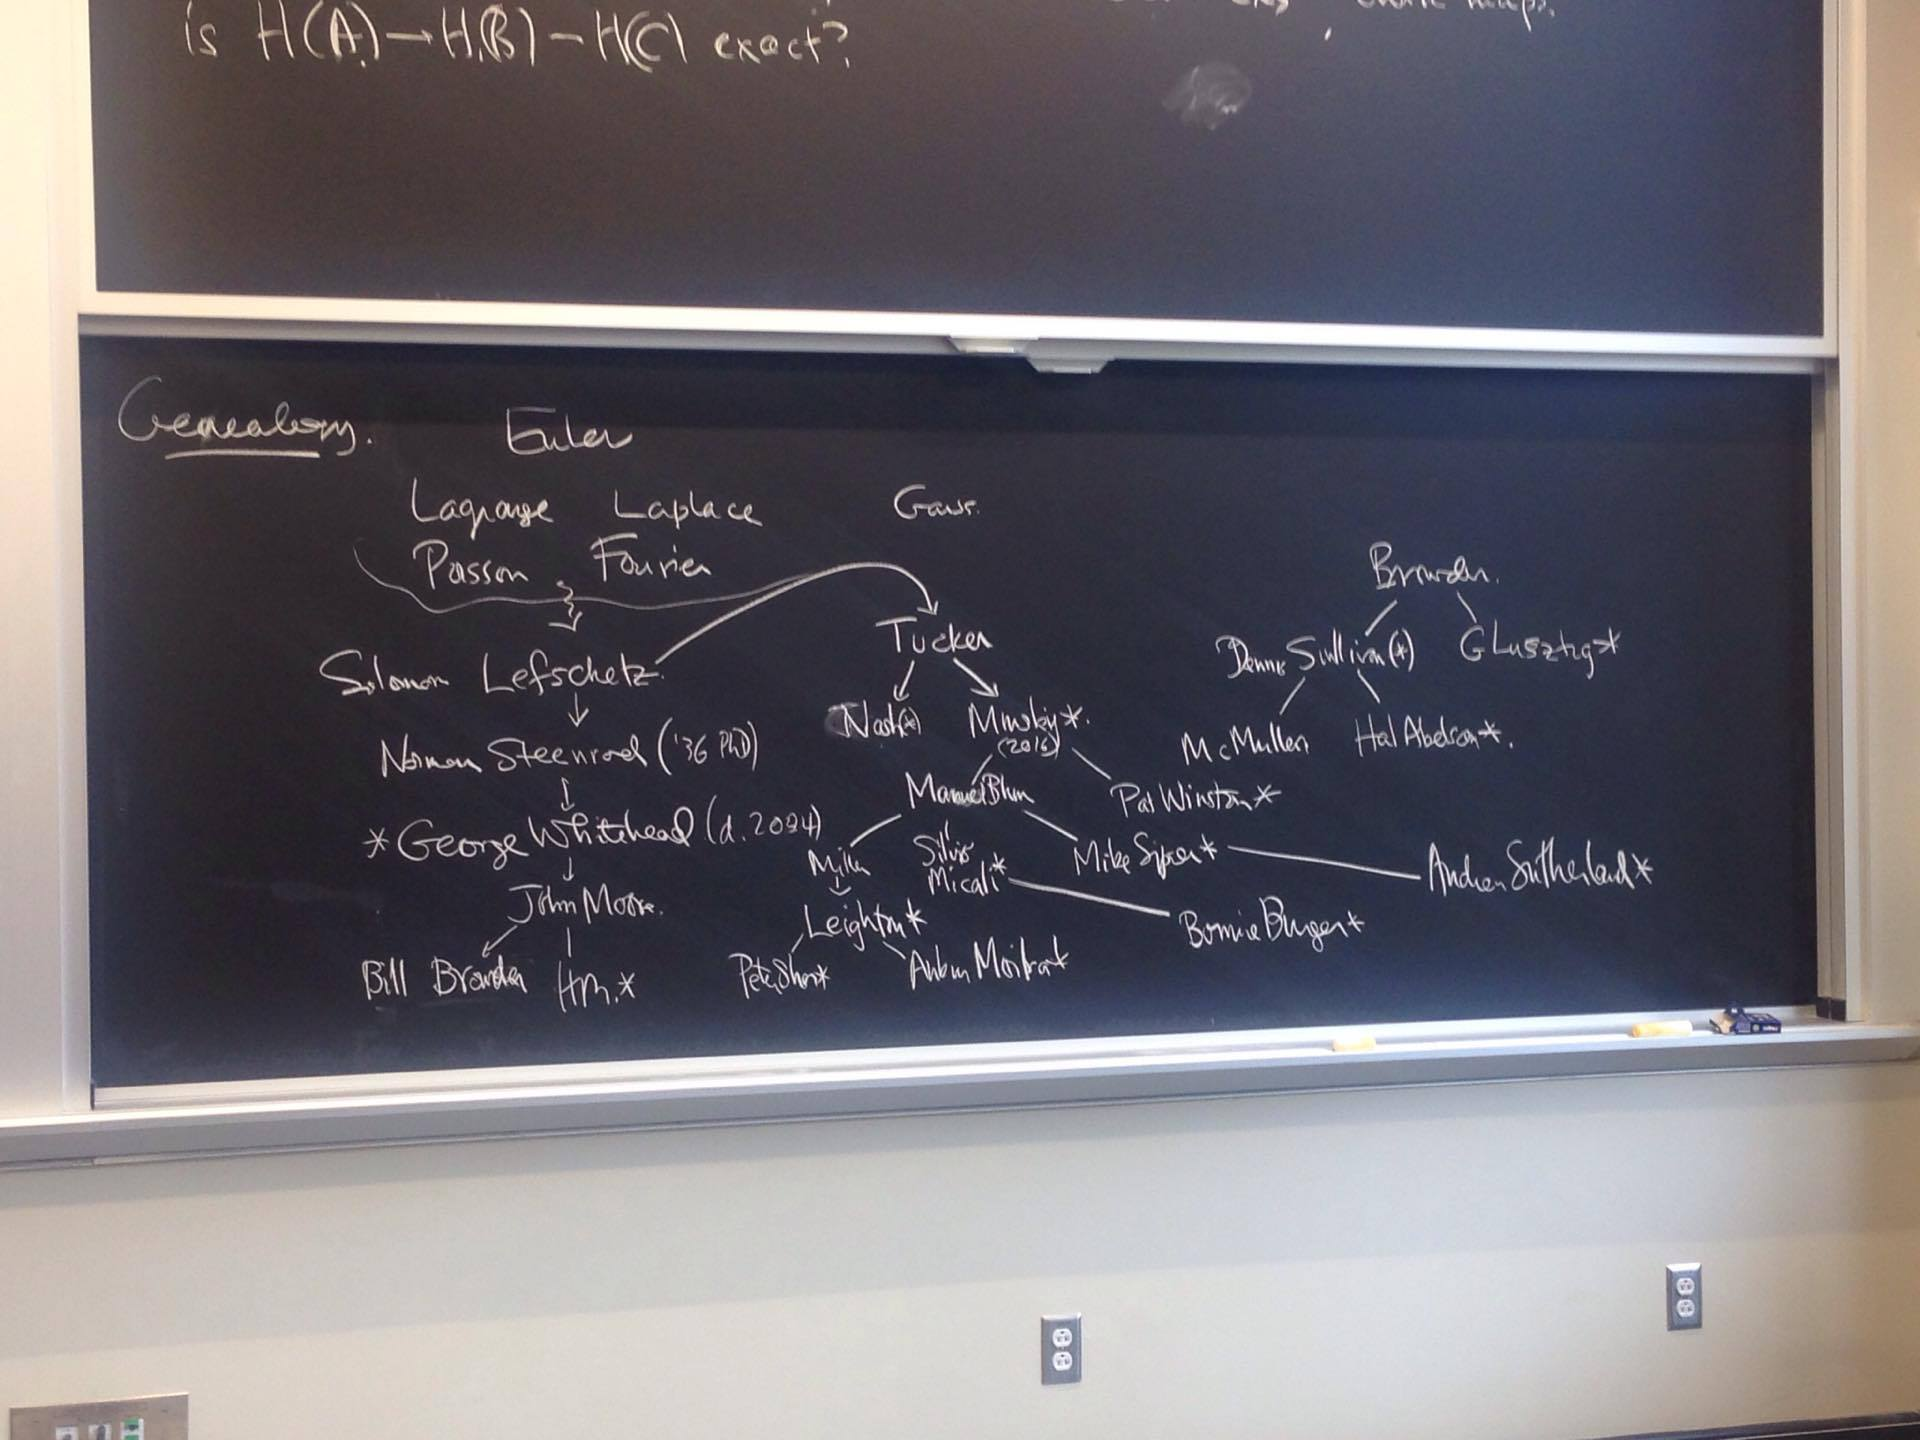
\includegraphics[width=\textwidth]{assets/math-family}
\caption{Mathematical genealogy, growing from Lefschetz, who was initially a chemist. The asterisks are meant to indicate that someone's at MIT.}
\end{figure}

\section{Excision, and the Eilenberg-Steenrod axioms}
We have homotopy invariance and the lexseq of a pair. We claimed that $ H_\ast(X,A)$ ``depends only on $X-A$''. You have to be careful about this. 
\begin{definition}
A triple $(X,A,U)$ where $U\subseteq A\subseteq X$ is \emph{excisive} if $\overline{U}\subseteq\mathrm{Int}(A)$. This is a point-set definition. From an excisive triple you can get a pair $(X-U,A-U)\subseteq (X,A)$, and this is called an exision.
\end{definition}
\begin{theorem}
An excision induces an isomorphism in homology, i.e., $ H_\ast(X-U,A-U)\cong H_\ast(X,A)$. We might prove this on Wednesday.
\end{theorem}
What are some consequences? We'll compute $ H_\ast(S^n)$ and $ H^\ast(D^n,S^{n-1})$. Here's the result. We'll use the homeomorphisms $D^n\simeq \Delta^n$ and $S^{n-1}\simeq\partial\Delta^n$. Let's write $S^0=\{0,1\}$, and $\iota_n:\Delta^n\to\Delta^n$.
\begin{theorem}
	\begin{enumerate}
	\item \begin{equation*}
	 H_q(S^n)=\begin{cases}\Z = \langle[c^0_\ast]\rangle & q=0,n>0\\ \Z\oplus\Z = \langle[c^0_1],[\partial\iota_1]\rangle & q=n=0 \\ \Z = \langle[\partial\iota_{n+1}]\rangle & q=n>0 \\ 0 & \text{else} \end{cases}
	\end{equation*}

	\item \begin{equation*}
	 H_q(D^n,S^{n-1}) = \begin{cases}
	\Z=\langle [\iota_n]\rangle & q=n\\
	0 & \text{else}
	\end{cases}
	\end{equation*}
	\end{enumerate}
\end{theorem}
If $n=0$, then we say that $S^{-1}=\emptyset$. What are the generators of these groups?
\begin{proof}
We'll use the lexseq, homotopy invariance, and excision. We have the lexseq:
\begin{equation*}
\xymatrix{ & & \ar[dll]^\partial\\
 H_q(S^{n-1})\ar[r] & H_q(D^n)\ar[r] & H_q(D^n,S^{n-1})\ar[dll]^\partial\\
 H_{1-1}(S^{n-1})\ar[r] & H_{q-1}(D^n)\ar[r] & H_{q-1}(D^n,S^{n-1})\ar[dll]^\partial\\
 & & &}
\end{equation*}
But we know that $D^n$ is contractible, so $ H_q(D^n)=\begin{cases}\Z & q=n\\ 0 & \text{else}\end{cases}$. This means that $\partial: H_q(D^n,S^{n-1})\cong H_{q-1}(S^{n-1})$ for $q>1$, but when $q=1$, we get $0\to H_1(D^n,S^{n-1})\xrightarrow{\partial} H_0(S^{n-1})\to H_0(D^n) \to H_0(D^n,S^{n-1})\to 0$.

Let's think about the case $n>1$. Then $ H_0(S^{n-1})=\mathbf{Z}=\langle[c^0_\ast]\rangle$, and $ H_0(D^n)=\Z=\langle[c^0_\ast]\rangle$, so you have an isomorphism, which means that $ H_0(D^n,S^{n-1})=0$ and $ H_1(D^n,S^{n-1})=0$. Now, let's go to the case $n=1$. Then $ H_0(S^0)=\Z\oplus\Z=\langle [c^0_\ast],[\partial\iota_1]\rangle$ and $ H_0(D^0)=\Z$. But $[\partial\iota_1]$ goes to zero, and $[c^0_\ast]$ goes to the generator of $\Z= H_0(D^0)$. This means that $ H_1(D^1,S^0)$ is generated by $\langle[\iota_1]\rangle\cong\Z$ because the map $ H_1(D^n,S^{n-1})\to H_0(S^{n-1})$ is the boundary map, so $[\iota_1]\mapsto [\partial\iota_1]$.

Excision will come into play through the following statement.
\begin{prop}
If $n>1,q>1$, then $ H_q(D^n,S^{n-1})\to H_q(D^n/S^{n-1},\ast)\cong H_q(S^n,\ast)\cong H_q(S^n)$, because $D^n/S^{n-1}\simeq S^n$. The claim is that this collapse map is an isomorphism.
\end{prop}
This provides the inductive step. Let's assume we've proved the proposition. Then $ H_q(D^n,S^{n-1})\cong H_{q-1}(S^{n-1})$. The proposition says that $ H_q(S^n)\cong H_{q-1}(S^{n-1})$. But we also have the boundary map $\partial: H_{q+1}(D^n,S^{n-1})\cong H_q(S^n)$, i.e., $ H_{q+1}(D^n,S^{n-1})\cong H_q(D^n,S^{n-1})$.

Now I want to prove the proposition. 
\begin{proof}[Proof of proposition]
We want to compare $ H_q(D^n,S^{n-1})$ and $ H_q(D^n/S^{n-1},\ast)$. We'll use excision to do this. We have $D^n=\{ x\in\mathbf{R}^{n+1} | |x|\leq 1 \}$. Let $A=\{ x|1/3\leq |x|\leq 1 \}$ and $U=\{ x|2/3<|x|\leq 1 \}$, and $\{ x||x|=1 \} =S^{n-1}\subseteq U$. We need a preliminary step. $ H_q(D^n,S^{n-1})\to H_q(D^n,A)$. We claim that this an isomorphism, but this is true because of the lexseq and the 5-lemma. By excision, $ H_q(D^n,A)\cong H_q(D^n-U,A-U)$. We can collapse the $(n-1)$-sphere, and $(D^n/S^{n-1}-U/S^{n-1},A/S^{n-1}-U/S^{n-1})=(D^n-U,A-U)$ because you're collapsing something from something that's already been collapsed! Now, we claim that $ H_q(D^n/S^{n-1}-U/S^{n-1},A/S^{n-1}-U/S^{n-1})\cong H_q(D^n/S^{n-1},A/S^{n-1})$, which is true by excision. THE FOLLOWING PART IS MOST DEFINITELY NOT RIGHT\footnote{My own comment: this proof can be finished by noticing that $A\simeq S^{n-1}$ via $\mathbf{v}\mapsto\frac{\mathbf{v}}{||\mathbf{v}||}$, and that $D^n/S^{n-1}\simeq S^n$.}. But also, $ H_q(D^n/S^{n-1},\text{disk})= H_q(D^n/S^{n-1},A/S^{n-1})$. Because the disk is contractible, using the lexseq and the 5-lemma completes the proof of the proposition.
\end{proof}
\end{proof}
``This really turns me on, because I love homology.'' Why should you care about homology?
\begin{corollary}
If $m\neq n$, then $S^m\not\simeq S^n$ because they have different homology groups. 
\end{corollary}
\begin{corollary}
If $m\neq n$, then $\mathbf{R}^m\not\cong \mathbf{R}^n$, because they're not homeomorphic.
\end{corollary}
\begin{proof}
Let $m,n>0$. Assume we have a homeomorphism $f:\mathbf{R}^m\to \mathbf{R}^n$. This restricts to $\mathbf{R}^m-\{0\}\to \mathbf{R}^n-\{0\}$, but each of these are homotopy equivalent to spheres, but we can't get a homotopy equivalence between two spheres of different dimension by the above corollary.
\end{proof}
\subsection{Eilenberg-Steenrod axioms}
\begin{definition}
A homology theory (on $\mathbf{Top}$) is:
\begin{itemize}
\item a functor $h_n:\mathbf{Top}_2\to\mathbf{Ab}$ for all $n$. We'll write $h_n(X)=h_n(X,\emptyset)$
\item natural transformations $\partial:h_n(X,A)\to h_{n-1}(A)$.
\end{itemize}
such that:
\begin{itemize}
\item if $f_0,f_1:(X,A)\to (Y,B)$ are homotopic, then $f{0,\ast}\simeq f_{1,\ast}:h_n(X,A)\to h_n(Y,B)$.
\item an excision induces isomorphisms.
\item a lexseq:
\begin{equation*}
\cdots\to h_{q+1}(X,A)\xrightarrow{\partial}h_q(A)\to h_q(X)\to h_q(X,A)\xrightarrow{\partial}\cdots
\end{equation*}
\item (the dimension axiom): $h_n(\ast)$ is nonzero only in dimension zero. This is like the parallel postulate.
\end{itemize}
\end{definition}
\begin{example}
Ordinary singular homology satisfies these. 
\end{example}
\begin{theorem}[Brouwer fixed-point theorem]
If $f:D^n\to D^n$, then there is some point $x\in D^n$ such that $f(x)=x$.
\end{theorem}
\begin{proof}
Suppose not. Then you can draw a ray from $x$ to $f(x)$ to the boundary $S^{n-1}$, intersecting at a point $g(x)$. Left to you to check that $g$ is continuous. If $x$ was on the boundary, then $x=g(x)$. This is inconsistent by our computation because otherwise the identity on $ H_{n-1}(S^{n-1})$ would be zero, contradiction!
\end{proof}

\section{Application of our previous calculation of $ H_\ast(S^n)$ and the ``locality principle''}
\begin{theorem}
Let $n\geq 1$. There is a surjective monoid homomorphism $[S^n,S^n]\to \Z_\times$, where $\Z_\times$ is the multiplicative monoid of $\Z$. $[S^n,S^n]$ is a monoid under composition. (This is basically the degree...)
\end{theorem}
\begin{proof}
Given $f:S^n\to S^n$, take the homology, which is just a homomorphism $\Z\to \Z$, all of which are simply multiplication by an integer. The integer by which you're multiplying to get this homomorphism is the integer associated to $f$.

Construction. If $n=1$, this is just the winding number. Suppose I've constructed this in dimension $n-1$. We have:
	\begin{equation*}
	\xymatrix{ H_{n-1}(S^{n-1})\ar[d]^n & \ar[l] H_n(D^n,S^{n-1})\ar[r]\ar[d] & H_n(S^n)\ar[d]\\
	 H_{n-1}(S^{n-1}) & \ar[l] H_n(D^n,S^{n-1})\ar[r] & H_n(S^n)}
	\end{equation*}
So we're basically suspending $f:S^{n-1}\to S^{n-1}$. More explicitly, if you have $f:S^{n-1}\to S^{n-1}$. We can extend to $\overline{f}:D^n\to D^n$ by sending $tx\mapsto tf(x)$ where $tx$ denotes the ray connecting $x\in S^{n-1}$ to the origin, and we can then quotient out by $S^{n-1}$ to get the map $S^n\to S^n$ as required.
\end{proof}
\subsection{Addendum to the ES axioms}
There's a further axiom, which isn't due to ES, but rather due to Milnor. It's this.
\begin{itemize}
\item Suppose $I$ a set. For each $\alpha\in I$ there's have a space $X_\alpha\in\mathbf{Top}$. I can consider $\coprod_\alpha X_\alpha$. There are inclusion maps $X_\alpha\to\coprod_\alpha X_\alpha$. Then $\bigoplus_\alpha h_n(X_\alpha)\cong h_n\left(\coprod_\alpha X_\alpha\right)$.
\end{itemize}
This is known for ordinary singular homology.
\subsection{Homological algebra}
\begin{enumerate}
\item Suppose $A,B\subseteq C$ are abelian groups. Then $A+C\subseteq C$. You have a sexseq $0\to A\cap B\to A\oplus B\to A+C\to 0$ where the map $c\mapsto (c,-c)$ is how the map $A\cap B\to A\oplus B$ is defined.
\item ``Fundamental isomorphism for abelian groups'' says the following. We have two sexseqs.
	\begin{equation*}
	\xymatrix{0\ar[r] & A\cap B\ar[r]\ar[d] & B\ar[r]\ar[d] & B/A\cap B\ar[r]\ar@{-->}[d]^\cong & 0\\
	0\ar[r] & A\ar[r] & A+B\ar[r] & (A+B)/A\ar[r] & 0}
	\end{equation*}
	I'm not going to write out the diagram chase that we did.
\item ``Snake lemma''. Suppose I have\footnote{``It's my Turn'', Jill Clayburgh}:
	\begin{equation*}
	\xymatrix{ & \ker f^\prime\ar[r]\ar[d] & \ker f\ar[r]\ar[d] & \ker f^{\prime\prime}\ar[d]\\
	0\ar[r] & A^\prime\ar[r]\ar[d]^{f^\prime} & A\ar[r]\ar[d]^f & A^{\prime\prime}\ar[r]\ar[d]^{f^{\prime\prime}} & 0\\
	0\ar[r] & B^\prime\ar[r]\ar[d] & B\ar[r]\ar[d] & B^{\prime\prime}\ar[r]\ar[d] & 0\\
	 & \coker f^\prime\ar[r] & \coker f\ar[r] & \coker f^{\prime\prime}}
	\end{equation*}
	Claim is that there's a map $\ker f^{\prime\prime}\to\coker f$ so that $0\to \ker f^\prime\to \ker f\to \ker f^{\prime\prime}\to\coker f^\prime\to\coker f\to \coker f^{\prime\prime}\to 0$. This is basically the lexseq in homology associated to the sexseqs of the following three chain complexes: $0\to A^\prime\to B^\prime\to 0$, $0\to A\to B\to 0$, and $0\to A^{\prime\prime}\to B^{\prime\prime}\to 0$. Work this out yourself.
\end{enumerate}
\subsection{Locality}
\begin{definition}
The (not necessarily open) cover of a topological space. Won't write this.
\end{definition}
\begin{definition}
Let ${\mathscr{A}}$ be a cover of $X$. An $n$-simplex $\sigma$ is ${\mathscr{A}}$-small if there is $A\in \mathscr{A}$ such that the image of $\sigma$ is entirely in $A$.
\end{definition}
Notice that if $\sigma:\Delta^n\to X$ is ${\mathscr{A}}$-small, then so is $d^i\sigma$. Let's denote by $\Sin^{\mathscr{A}}_n(X)$ the set of ${\mathscr{A}}$-small $n$-simplices. This means that we get a map $\Sin^{\mathscr{A}}_n(X)\to \Sin^{\mathscr{A}}_{n-1}(X)$. Let $S^{\mathscr{A}}_n(X)=\Z[\Sin^{\mathscr{A}}_n(X)]$. Then there's a subchain complex $S^{\mathscr{A}}_\ast(X)$.
\begin{theorem}
The inclusion $S^\mathscr{A}_\ast(X)\subseteq S_\ast(X)$ is a chain homotopy equivalence.
\end{theorem}
\begin{corollary}
If $ H^\mathscr{A}_\ast(X):= H(S^\mathscr{A}_\ast(X))$, then $ H^\mathscr{A}_\ast(X)\cong H_\ast(X)$.
\end{corollary}
We'll do this on Monday.
\begin{example}
If $\mathscr{A}=\{A,B\}$, then $\overline{X-B}=X-\mathrm{Int}(B)\subseteq\mathrm{Int}(A)$. Let $X-B=U$. Then $U\subseteq \overline{U}\subseteq \mathrm{Int}(A)\subseteq A\subseteq X$. This is an excision! So $U\subseteq A\subseteq X$ is an excision. But now, $(X-U,A-U)\to (X,A)$ is an excision, but $(X-U,A-U)=(B,A\cap B)$, so we have $(B,A\cap B)\to (X,A)$ is an excision. Now, also, $S^\mathscr{A}_\ast(X)=S_\ast(A)+S_\ast(B)$. Says he got off track, let me just write things out and explain in a moment.
\begin{equation*}
	\xymatrix{0\ar[r] & S_n(A)\cap S_n(B)=S_n(A\cap B)\ar[r]\ar[d] & S_n(B)\ar[r]\ar[d] & S_n(B,A\cap B)\ar[r]\ar@{-->}[d]^\cong & 0\\
	0\ar[r] & S_n(A)\ar[r] & S_n(A)+S_n(B)=S^\mathscr{A}_n(X)\ar[r] & S^\mathscr{A}_n(X)/S_n(A)\ar[r] & 0}
	\end{equation*}
But we can consider $S_\ast(X)/S_\ast(A)=S_\ast(X,A)$. By the lexseq + 5 lemma, this thing is isomorphic to $S^\mathscr{A}_n(X)/S_n(A)$, so $S_\ast(B,A\cap B)\cong S_\ast(X,A)$ in homology. This is precisely the excision theorem. QED.
\end{example}

\section{Mayer-Vietoris and Subdivision}
(Is it Meyer-Vietoris or Mayer-Vietoris?) Today is the lecture with a lot of formulae.
\begin{theorem}
Let $\sca$ be a cover of $X$, so that $X=\bigcup_{A\in \sca}\mathrm{Int}(A)$. Then the theorem we're going to prove is this. If $S^\sca_\ast(X)=\sum_{A\in\sca}S_\ast(A)\to S_\ast(X)$ induces an isomorphism in $ H_\ast$. (This is a ``quasi-isomorphism'' of chain complexes.)
\end{theorem}
Because this lecture's full of formulas, I'm going to stand around with a piece of paper in my hand.
\begin{example}
Let $\sca=\{A,B\}$ of X, so that:
\begin{equation*}
\xymatrix{A\cap B\ar[r]^{j_1}\ar[d]^{j_2} & A\ar[d]^{i_1}\\
B\ar[r]_{i_2} & X}
\end{equation*}
Then consider the following diagram:
\begin{equation*}
\xymatrix{0\ar[r] & S_\ast(A\cap B)\ar[r]^{\begin{pmatrix}j_{1\ast} \\ -j_{2\ast}\end{pmatrix}}\ar@{=}[d] & S_\ast(A)\oplus S_\ast(B)\ar[r]\ar[d] & S^\sca_\ast(X)\ar[r]\ar@{=}[d] & 0\\
0\ar[r] & S_\ast(A)\cap S_\ast(B)\ar[r] & S_\ast(A)\oplus S_\ast(B)\ar[dr]\ar[r]^{(i_{1\ast},\ i_{2\ast})} & S_\ast(A)+S_\ast(B)\ar[r]\ar@{^(->}[d] & 0\\
 & & & S_\ast(X) &}
\end{equation*}
The map $S_\ast(A)+S_\ast(B)\hookrightarrow S_\ast(X)$ is a quasi-isomorphism, this is what locality says. Take the homology of this to get a lexseq:
\begin{equation*}
\xymatrix{ \cdots\ar[rr] & & H_{n+1}(X)\ar[dll]_{\begin{pmatrix}j_{1\ast} \\ -j_{2\ast}\end{pmatrix}}\\
 H_n(A\cap B)\ar[r] & H_n(A)\oplus H_n(B)\ar[r]^{(i_{1\ast},\ i_{2\ast})} & H_n(X)\ar[dll]\\
 H_{n-1}(A\cap B)\ar[r] & H_{n-1}(A)\oplus H_{n-1}(B)\ar[r] & \cdots}
\end{equation*}
Voila, you have Mayer-Vietoris. (I have a different proof of this that I submitted in homework.)
\end{example}
\subsection{The cone construction}
Let $X\subseteq \mathbf{R}^N$ be a star-shaped region, and let $b\in\mathbf{R}^N$. Then we showed that the augmentation $S_\ast(X)\xrightarrow{\epsilon}\Z$ is a chain homotopy equivalence. There's another map going backwards $\Z\xrightarrow{\eta_b} S_\ast(X)$ sending $1\mapsto c^0_b$. Clearly the composition $\epsilon\circ\eta_b$ is the identity. We want to show that $\eta_b$ ad $\epsilon$ are chain homotopy inverses to each other. One direction is easy. The other map $S_\ast(X)\xrightarrow{\eta_b\epsilon}S_\ast(X)$ being homotopic to $1_{S_\ast(X)}$ is a little harder. This means that we want to construct a map $b\ast:S_n(X)\to S_{n+1}(X)$ such that $db\ast+b\ast d=1-\eta_b\epsilon$.

Consider some $\sigma:\Delta^1\to X$. Then because $X$ is star shaped, you can send $\sigma$ to $b$. This gives a $2$-simplex $b\ast \sigma$, called the \emph{join}. We'll define this $2$-simplex and label it so that the zero vertex is $b$ itself, the $1$ vertex is $d_1\sigma$, and the $2$ vertex is $d_0\sigma$. Define $b\ast\sigma$ as follows (where $(t_0,\cdots,t_{n+1})\in \Delta^{n+1}$):
\begin{equation*}
b\ast\sigma(t_0,\cdots,t_n,t_{n+1})=t_0b + (1-t_0)\sigma\left(\frac{t_1,\cdots,t_{n+1}}{1-t_0}\right)
\end{equation*}
When $t_0=0$, then you recover exactly $\sigma(t_1,\cdots,t_{n+1})$ and when $t_0=1$, this is exactly $b$. (Why can you divide by $1-t_0=0$?) This is a map $b\ast:\Sin_n(X)\to\Sin_{n+1}(X)$, so we can extend linearly to get $S_n(X)\to S_{n+1}(X)$, also denoted $b\ast$. What is $d_i(b\ast\sigma)$? This is exactly:
\begin{equation*}
d_i(b\ast\sigma)=\begin{cases}\sigma & i=0 \\ 
c^0_b & i=1,n=0\\
b\ast d_{i-1}\sigma & i>0,n>0\end{cases}
\end{equation*}
The latter thing seems true because in the case when $n=1$, $d_2(b\ast\sigma)$ is the cone on $d_1\sigma$. The middle thing is true because when $n=0$ you can't use the bottom thing (what is the boundary in that case?), and if you draw this out, noting our convention that when $t_0=1$ you have $d_1\sigma$ and when $t_0=1$ you have $b$, this automatically yields $d_1(b\ast\sigma)=b$ if $\sigma:\Delta^0\to X$. We can rewrite this as follows. Here $c\in S_n(X)$.
\begin{equation*}
d_i(b\ast c)=\begin{cases}
c & i=0\\
b\ast d_0c + \eta_b\epsilon c & i=1\\
b\ast d_{i-1}\sigma & i>1
\end{cases}
\end{equation*}
Because $d_0$ of a $0$-simplex is defined to be zero. This may seem confusing, but it's just a translation of what we wrote down above. We want to compute that this thing is actually a chain homotopy. Let's compute.
\begin{align*}
d(b\ast c)& = d_0(b\ast c) - d_1(b\ast c) + \sum_{i>1}(-1)^i d_i(b\ast c)\\
& = c-(b\ast d_0c + \eta_b\epsilon c) + \sum_{i=2}^n (-1)^ib\ast d_{i-1}c\\
& = c-\eta_b\epsilon c - \sum_{j=0}^{n-1}(-1)^jb\ast d_jc\\
& = c-\eta_b\epsilon c - b\ast dc
\end{align*}
Here $j=i-1$. The equality $\sum_{j=0}^{n-1}(-1)^jb\ast d_jc=b_\ast dc$ holds because $b\ast$ is linear (by definition on $S_n(X)$). This means that $b\ast$ is a chain homotopy, QED. This completes what we've claimed about the star shaped region. We want to use this cone construction to talk about subdivision.
\subsection{Subdivide the standard simplex}
Let's focus on the standard simplex. This is a nice thing about singular homology. For the $1$-simplex, you just cut in half. For the $2$-simplex, just look at the subdivision of each face, and look at the barycenter\footnote{The barycenter of the $n$-simplex is $b_n:=\frac{(1,\cdots,1)}{n+1}$.}, and join the barycenter to the $1$-simplex between each ``half'' $1$-simplex. We want to formalize this process. Define a natural transformation $\$:S_n(X)\to S_n(X)$ by defining on standard $n$-simplex, namely by specifying what $\$(\iota_n)$ is where $\iota_n:\Delta^n\xrightarrow{\mathrm{id}}\Delta^n$, and then extending by naturality (namely $\$(\sigma)=\sigma_\ast\$(\iota_n)$). Here's the definition. When $n=0$, define $\$=\mathrm{id}$, i.e., $\$(\iota_0)=\iota_0$. For $n>0$, define $\$\iota_n:=b_n\ast\$ d\iota_n$ where $b_n$ is the barycenter of $\Delta^n$. This makes a \emph{lot} of sense if you draw out a picture, and it's a very clever definition that captures the geometry we described. Let me tell you what we'll prove about this, most likely on Wednesday.
\begin{prop}
$\$$ is a chain map $S_\ast(X)\to S_\ast(X)$, i.e., $\$d=d\$$. Also, $\$\simeq 1$.
\end{prop}
Also, class is cancelled on Friday.

\section{Locality (almost done!)}
\begin{theorem}
We discovered that $S^\sca_\ast(X)\hookrightarrow S_\ast(X)$ is a subcomplex, and this induced an isomorphism in homology.
\end{theorem}
We talked about subdivision and the cone construction, the latter of which dealt with a star-shaped region, relative to some point (which we can safely assume is the origin) $b$. If $\sigma:\Delta^n\to X$ is a map, then $b\ast \sigma:S_n(X)\to S_{n+1}(X)$ where $\ast$ is the join. We did all of this before. The property that this had is that it's a homotopy between $1$ and $\eta_b\epsilon$, i.e., $db\ast + b\ast d = 1-\eta_b\epsilon$. This is called equation $(\ast)$. Look above for the definition of $\eta_b$ and $\epsilon$. Hopefully you remember this story.

The subdivision operator $\$:S_\ast(X)\to S_\ast(X)$ for any space $X$ is natural, so it's enough to say what $\$\iota_n$ and $\$\iota_0$ is. Define $\$\iota_0=\iota_0$, and define $\$\iota_n=b_n\ast\$(d\iota_{n-1})$ where $b_n$ is the barycenter of the $n$-simplex. The standard simplex is star-shaped relative to its barycenter, so by naturality, it suffices to do this for $\iota_n$. The two key properties are the following.
\begin{theorem}
\begin{enumerate}
\item $\$$ is a chain map.
\item There is a chain homotopy $T:\$\sim 1$.
\end{enumerate}
\end{theorem}
\begin{proof}
Let's try to prove that it's a chain map. We'll use induction on $n$. It's enough to show that $d\$\iota_n=\$ d\iota_n$, because:$$d\$\sigma=d\$\sigma_\ast\iota_n=\sigma_\ast d\$\iota_n=\sigma_\ast \$d\iota_n=\$ d\sigma_\ast\iota_n=\$ d\sigma$$
We declared $d\$\iota_0=d\iota_0=0$. But also $\$d\iota_0=\$0=0$, so this works.

For $n\geq 1$, we want to compute $d\$\iota_n$. This is:
\begin{align*}
d\$\iota_n & =d(b_n\ast \$ d\iota_n) & \\
 & = (1-\eta_b\epsilon-b_n\ast d)(\$ d\iota_n) & \text{by $(\ast)$}
\end{align*}
What happens when $n=1$? Well:
$$\eta_b\epsilon\$d\iota_1 = \eta_b\epsilon \$(c^0_1 - c^0_0)=\eta_b\epsilon(c^0_1 - c^0-0)=0$$
Because $\epsilon$ takes sums of coefficients, which is $1+(-1)=0$. Let's continue.
\begin{align*}
d\$\iota_n & = ... & \\
 & = \$d\iota_n - b_n\ast d\$ d\iota_n & \\
 & = \$d\iota_n - b_n\$d^2\iota_n &\\
 & = \$d\iota_n & \text{because $d^2=0$}
\end{align*}
So we're done.

To define the chain homotopy $T$, we'll just write down a formula and not justify it. We just need to define $T\iota_n$ by naturality. So define:
\begin{equation*}
T\iota_n = \begin{cases}
0 & n=0\\
b_{n}\ast(\$\iota_n - \iota_n- Td\iota_n)\in S_{n+1}(\Delta^n) & n>0
\end{cases}
\end{equation*}
This is because $T:S_n(X)\to S_{n+1}(X)$ such that $dT+Td=\$-1$. I'm confused about this, so help me out. Hmm. The term $\$\iota_n - \iota_n-Td\iota_n$ is an $n$-chain. We're going to do this by induction. Again, we need to check only on the universal case.

When $n=0$, $dT\iota_0 + Td\iota_0 = 0+0 = 0 = \$\iota_0 - \iota_0$ because $\$\iota_0=\iota_0$. Now let's induct. For $n\geq 1$, let's start by computing $dT\iota_n$. This is:
\begin{align*}
dT\iota_n & = d_n(b_n\ast(\$\iota_n - \iota_n - Td\iota_n)) & \\
& = (1-b_n\ast d)(\$\iota_n - \iota_n - Td\iota_n) & \text{by $(\ast)$}\\
 & = \$\iota_n-\iota_n-Td\iota_n-b_n\ast (d\$\iota_n - d\iota_n - dTd\iota_n)
\end{align*}
We can ignore the $\eta_b\epsilon$ part because we're in dimension $\geq 1$. All we want now is that $b_n\ast(d\$\iota_n - d\iota_n - dTd\iota_n)=0$. We can do this via induction, because $T(d\iota_n)$ is in dimension $n$ (or is it $n-1$?):
\begin{align*}
dTd\iota_n & = -Td(d\iota_b)+\$ d\iota_n - d\iota_n\\
& = \$d\iota_n - d\iota_n\\
& = d\$\iota_n - d\iota_n
\end{align*}
This means that $d\$\iota_n-d\iota_n - dTd\iota_n=0$, so we're done.
\end{proof}
\begin{corollary}
$\$^k\sim 1:S_\ast(X)\to S_\ast(X)$. I.e., we're iterating subdivision. We want $T_k$ such that $dT_k+T_kd=\$^k-1$
\end{corollary}
\begin{proof}
$dT+Td=\$-1$. Let's apply $\$$ to this. We get $\$dT+\$Td=\$^2-\$$. Sum up these two things, so we get $dT+Td+\$dT+\$Td = \$^2-1$. But now, $\$d=d\$$, so the left hand side is $dT+d\$T + Td+\$Td = d(\$+1)T + (\$+1)Td$, i.e., $d(\$+1)T+(\$+1)Td=\$^2-1$. So define $T_2=(\$+1)T$, and continuing, you see that $T_k=(\$^{k-1}+\$^{k-2}+\cdots+1)T=\left(\sum^{k-1}_{i=0}\$^i\right)T$.
\end{proof}
\begin{prop}[Almost completes the proof of locality]
Let $\sca$ be a cover of $X$. For every chain $c\in S_n(X)$, there is a $k\geq 0$ such that $\$^kc\in S^\sca_n(X)$. This is the geometric thing we have to prove.
\end{prop}
\begin{proof}
We may assume that $c:\sigma:\Delta^n\to X$, and this makes sense because you just take the max of the $k$ of the terms of the sum. A great trick is the following: define an open cover $\mathscr{U}$ of $\Delta^n$ defined by $\mathscr{U}:=\{\sigma^{-1}(\mathrm{Int}(A))|A\in\sca\}$. This is a cover, a basic result from topology. Then we use the Lesbegue covering lemma:
\begin{lemma}[Lesbegue covering lemma]
We'll pretend this is part of 18.901. Let $M$ be a compact metric space (eg. $\Delta^n$), and let $\mathscr{U}$ be an open cover. Then there is $\epsilon> 0$ such that for all $x\in M$, there is $B_\epsilon(x)\subseteq U$ for some $U\in \mathscr{U}$.
\end{lemma}
\begin{proof}
Omitted, may be in 18.901. Or even 18.100B.
\end{proof}
Let's apply this to the cover we constructed. What we want is that for all $\epsilon>0$, there is a $k$ such that the diameter of the simplices in $\$^k\iota_n$ is less than $\epsilon$. Let's do that.
\begin{question}
How small are these subdivided simplices in $\$^k\iota_n$?
\end{question}
For example, suppose $\sigma:\Delta^n\to\Delta^n$ is something in the subdivision. These are all affine simplexes, i.e., it's determined by where the simplices of $\Delta^n$ go to in $\sigma$. We can write $\sigma=\langle v_,\cdots,v_n\rangle$. It could be in $\mathbf{R}^N$ if you wanted; maybe it's easier to think of it this way. The barycenter is $\frac{\sum_{i=0}^nv_i}{n+1}$. Let's compute:
\begin{align*}
|b-v_i| & =\left|\frac{v_0+\cdots+v_n-(n+1)v_i}{n+1}\right|\\
& =\left|\frac{(v_0-v_i)+(v_1-v_i)+\cdots+(v_n-v_i)}{n+1}\right|\\
 & \leq \frac{n}{n+1}\max_{i,j}|v_i-v_j|\\
 & = \frac{n}{n+1}\mathrm{diam}(\img\sigma)
\end{align*}
The following lemma completes the proof because there's always a $k$ such that $\left(\frac{n}{n+1}\right)^k<\epsilon$.
\begin{lemma}
Let $\tau$ be a simplex in $\$^k\sigma$ where $\sigma$ is an affine simplex. Then $\mathrm{diam}(\tau)\leq \frac{n}{n+1}\mathrm{diam}(\sigma)$.
\end{lemma}
\begin{proof}
Let's write $\tau=\langle w_0=b,\cdots,w_n\rangle$ and $\sigma=\langle v_0,\cdots,v_n\rangle$. We saw:
\begin{align*}
|b-w_i| & \leq\max_i|b-v_i|\\
 & \leq \frac{n}{n+1}\mathrm{diam}(\sigma)
\end{align*}
For the other cases, well, we use induction:
\begin{align*}
|w_i-w_j|& \leq \mathrm{diam}(\text{simplex in }\$d\sigma)\\
& \leq \frac{n-1}{n}\mathrm{diam}(d\sigma)\\
& \leq \frac{n}{n+1}\mathrm{diam}(\sigma)
\end{align*}
We're almost there. We'll finish the proof of locality on Friday.
\end{proof}
\end{proof}

\section{Concluding Locality! and CW-complexes}
Again recall what $\sca$-small covers, etc. are. We want to prove that:
\begin{theorem}
$S^\sca_\ast(X)\hookrightarrow S_\ast(X)$ is a quasi-isomorphism, i.e., an isomorphism on homology.
\end{theorem}
We developed the subdivision operator $\$^k:S_\ast(X)\to S_\ast(X)$, and proved that it's a chain map. We showed that $T_k:\$^k\sim 1$.
\begin{proof}[Proof of locality]
We want to prove surjectivity of $ H_n(S^\sca_\ast(X))\to H_n(S_\ast(X))= H_n(X)$. Let $c\in Z_n(C_\bullet)(X)$. We want to find an $\sca$-small $n$-cycle that is homologous to $c$. There's only one thing to do. Pick $k$ such that $\$^k c$ is $\sca$-small. This is a cycle because $d\$^k c=\$^k dc=0$ because $\$^k$ is a chain map. I want to compare this new cycle with $c$. Consider the chain homotopy $T_k$; then: $dT_k c+T_kdc=\$^kc-c$. But $dc=0$, so $\$^k c - c=dT_k c$, so they differ by a boundary, and they're homologous.

Now for injectivity. Suppose $c\in S^\sca_n(X)$ with $dc=0$. Suppose that $c=db$ for some $b\in S_{n+1}(X)$, not necessarily $\sca$-small. We want $c$ to be a boundary of an $\sca$-small chain. Well:
\begin{align*}
& dT_kb+T_kdb=\$^k b-b\\
\Rightarrow& dT_kb+T_kc=\$^k b-b\\
\Rightarrow& d(dT_kb+T_kc)=\$^kb-b=dT_kc=d\$^k b-c\\
\Rightarrow& c=d\$^kb-dT_kc=d(\$^k b-T_kc)
\end{align*}
Now, $\$^k$ is $\sca$-small. Is $T_kc$ also $\sca$-small? I claim that it is. Why? It is enough to show that $T_k\sigma$ is $\sca$-small if $\sigma$ is. We know that $\sigma=\sigma_\ast\iota_n$. Because $\sigma$ is $\sca$-small, we know that $\sigma:\Delta^n\to X$ is the composition $i_\ast\overline{\sigma}$ where $\overline{\sigma}:\Delta^n\to A$ and $i:A\to X$ is the inclusion for some $A\in\sca$. This means that $T_k\sigma=T_ki_\ast\overline{\sigma}=i_\ast T_k\overline{\sigma}$, which certainly is $\sca$-small.
\end{proof}
``Are you happy? You should be very happy, because we've finished our first portion of this course. We now have a whole package of homology.''
\subsection{CW-complexes}
Simplicial complexes are rigid and combinatorial. But manifolds are smooth. In between, you have CW-complexes. (A lot of advertisement for this.) We want to ``glue'' things. This is the pushout construction. Namely, if you have $i:A\hookrightarrow B$ and $f:A\to X$, then you define $X\cup_f B$ (or $X\cup_A B$) via:
\begin{equation*}
\xymatrix{A\ar[r]^f\ar@{^(->}[d]_i & X\ar[d]\\
B\ar[r] & X\cup_f B}
\end{equation*}
defined by $X\cup_f B=X\sqcup B/\sim$ where $\forall a\in A$, $f(a)\sim a$. This is $X$ with $B$ attached along $f$. There are two kinds of equivalence classes, namely elements of $B-A$, because anything not in $A$ is just a singleton. The other is $\{x\}\cup f^{-1}(x)$ for $x\in X$, because anything that's not in $\img f$ is a singleton, but if something is in $\img f$, you identify it with its preimage. This is what it is as a set. It has a universal property. Suppose you have another space $Y$.
\begin{equation*}
\xymatrix{A\ar[r]^f\ar@{^(->}[d]_i & X\ar[d]^j\ar[ddr]^{\overline{j}} & \\
B\ar[r]\ar[drr]_{\overline{g}} & X\cup_f B\ar@{-->}[dr] & \\
 & & Y}
\end{equation*}
such that $\overline{j}f=\overline{g}i$. The topology is right too because that's what the quotient topology does for you. As I wrote before, this is called a \emph{pushout} of the following diagram:
\begin{equation*}
\xymatrix{A\ar[r]^f\ar@{^(->}[d]_i & X\\
B &}
\end{equation*}
\begin{example}
Let $X=\ast$. Then you have a pushout:
\begin{equation*}
\xymatrix{A\ar[r]^f\ar@{^(->}[d]_i & \ast\ar[d]\\
B\ar[r] & \ast\cup_f B}
\end{equation*}
So then $\ast\cup_f B=B/A$.
\end{example}
\begin{example}
\begin{equation*}
\xymatrix{\emptyset\ar[r]^f\ar@{^(->}[d]_i & X\ar[d]\\
B\ar[r] & X\cup_f B}
\end{equation*}
It's then clear that this is exactly $X\sqcup B$.
\end{example}
\begin{example}
If both:
\begin{equation*}
\xymatrix{\emptyset\ar[r]^f\ar@{^(->}[d]_i & \ast\ar[d]\\
B\ar[r] & \ast\cup_f B}
\end{equation*}
So $B/\emptyset=\ast\sqcup B$. For example, $\emptyset/\emptyset=\ast$. This is ``creation from nothing''. ``We won't get into the religious ramifications.''
\end{example}
\begin{example}[Attaching a cell, the most important]
Consider:
\begin{equation*}
\xymatrix{S^{n-1}\ar[r]^f\ar@{^(->}[d]_i & X\ar[d]\\
D^n\ar[r] & X\cup_f D^n}
\end{equation*}
This is called attaching a ``cell''. The $D^n$ is what's called a cell. You're attaching a contractible space. You might want to generalize this a little bit:
\begin{equation*}
\xymatrix{\coprod_{\alpha\in A}S^{n-1}_\alpha\ar[r]^f\ar@{^(->}[d]_i & X\ar[d]\\
\coprod_{\alpha\in A}D^n_\alpha\ar[r] & X\cup_f \coprod_{\alpha\in A}D^n_\alpha}
\end{equation*}
\end{example}
What are some examples? When $n=0$, the declaration is that $S^{-1}=\emptyset$, so this is:
\begin{equation*}
\xymatrix{\emptyset\ar[r]^f\ar@{^(->}[d]_i & X\ar[d]\\
\coprod_{\alpha\in A}\ast\ar[r] & X\cup_f \coprod_{\alpha\in A}\ast}
\end{equation*}
You're just adding a bunch of points to $X$. This is a little more interesting. What about:
\begin{equation*}
\xymatrix{S^0\sqcup S^0\ar[r]^f\ar@{^(->}[d]_i & \ast\ar[d]\\
D^1\sqcup D^1\ar[r] & \ast\cup_f (D^1\sqcup D^1)}
\end{equation*}
Then $\ast\cup_f(D^1\sqcup D^1)$ is a figure $8$, because you have two $1$-disks, where you identify the four boundary points together. If we consider $(X,\ast),(Y,\ast)$, then $X\vee Y:= X\sqcup Y/\ast\sim \ast$. So $\ast\cup_f(D^1\sqcup D^1)=S^1\vee S^1$. More interestingly:
\begin{equation*}
\xymatrix{S^1\ar[r]^{aba^{-1}b^{-1}}\ar@{^(->}[d]_i & S^1\vee S^1\ar[d]\\
D^2\ar[r] & (S^1\vee S^1)\cup_f D^2}
\end{equation*}
This is exactly the torus, i.e., $(S^1\vee S^1)\cup_f D^2=T^2$.
\begin{definition}
A \emph{CW-complex} is a space $X$ with a sequence of subspaces $\emptyset=X_{-1}\subseteq X_0\subseteq X_1\subseteq\cdots\subseteq X$ (could be an infinite sequence) such that for all $n$, there is a pushout diagram like this:
\begin{equation*}
\xymatrix{\coprod_{\alpha\in A_n}S^{n-1}_\alpha\ar[r]^f\ar@{^(->}[d]_i & X_{n-1}\ar[d]\\
\coprod_{\alpha\in A_n}D^n_\alpha\ar[r] & X_{n}}
\end{equation*}
And $X=\bigcup X_n$, topologically (i.e. $A\subseteq X$ is open if and only if $A\cap X_n$ is open for all $n$). Often, $X_n=\mathrm{Sk}_n(X)$, called the $n$-skeleton, in honor of Halloween (coming right up!), of $X$.
\end{definition}
\begin{example}
The torus is $\emptyset\subseteq T^2_0\subseteq T^2_1\subseteq T^2$. Here, $T^2_0=\ast$ and $T^2_1=S^1\vee S^1$.
\end{example}
\begin{definition}
A CW-complex is \emph{finite-dimensional} if $X_n=X$ for some $n$. Say that $X$ is of \emph{finite type} if each $A_n$ is finite, i.e., finitely many cell in each dimension. Say that $X$ is \emph{finite} if it's finite-dimensional and of finite type.
\end{definition}
In CW, the C is for cell, and the W is for weak, because of the topology on a CW-complex. This definition is due to J. H. C. Whitehead. Some people say that the ``CW'' comes from his name.
\begin{theorem}
\begin{enumerate}
\item Any CW-complex is Hausdorff, and it's compact if and only if it's finite.
\item Any compact smooth manifold admits a CW structure.
\end{enumerate}
\end{theorem}
\begin{proof}
Not going to do this.
\end{proof}
Note that there could be multiple CW-structures on something.

\section{CW-complexes and cellular homology}
Recall:
\begin{definition}
A \emph{CW-complex} is a space $X$ with a sequence of subspaces $\emptyset=X_{-1}\subseteq X_0\subseteq X_1\subseteq\cdots\subseteq X$ (could be an infinite sequence) such that for all $n$, there is a map $f:\coprod_{\alpha\in A_n}S^{n-1}_\alpha\to X_{n-1}$ (called the \emph{attaching map}), such that there is a pushout diagram like this:
\begin{equation*}
\xymatrix{\coprod_{\alpha\in A_n}S^{n-1}_\alpha\ar[r]^f\ar@{^(->}[d]_i & X_{n-1}\ar[d]\\
\coprod_{\alpha\in A_n}D^n_\alpha\ar[r] & X_{n}}
\end{equation*}
And $X=\bigcup X_n$, topologically (i.e. $A\subseteq X$ is open if and only if $A\cap X_n$ is open for all $n$). Often, $X_n$ is written $\mathrm{Sk}_n(X)$, and is called the $n$-skeleton of $X$.
\end{definition}
\begin{remark}
This means that if you ignore the topology, i.e., as sets: $X=\coprod_{n\geq 0}\left(\coprod_{\alpha\in A_n}\mathrm{Int}(D^n_\alpha)\right)$ where $\mathrm{Int}(D^n)=\{x\in D^n: |x|<1\}$ (the interior of $D^n$), so that $\mathrm{Int}(D^0)=D^0=\ast$. The $\mathrm{Int}(D^n_\alpha)$ are called ``open $n$-cells''. Note that the open $n$-cells are not generally open in the topology on $X$.
\end{remark}
\begin{example}
The $n$-sphere $S^n$. Let $\mathrm{Sk}_0(S^n)=\ast=\mathrm{Sk}_1(S^n)=\cdots=\mathrm{Sk}_{n-1}(S^n)\subseteq \mathrm{Sk}_n(S^n)=S^n$. We attach it by using the pushout:
\begin{equation*}
\xymatrix{S^{n-1}\ar[d]\ar[r] & \ast\ar@{^(->}[d]\\
D^n\ar[r] & S^n}
\end{equation*}
Here's another CW-structure. Let $\mathrm{Sk}_0(S^n)=S^0=S^n\cap \mathbf{R}^1\langle \mathbf{e}_1\rangle$, $\mathrm{Sk}_1(S^n)=S^{1}=S^n\cap\mathbf\mathbf{R}\langle \mathbf{e}_1,\mathbf{e}_2\rangle$, $\mathrm{Sk}_2(S^n)=S^2=S^n\cap\mathbf{R}\langle \mathbf{e}_1,\mathbf{e}_2,\mathbf{e}_3\rangle$, etc. until $\mathrm{Sk}_n(S^n)=S^n$. I have to give maps $u,\ell:D^k\to S^k$ so that you have a pushout:
\begin{equation*}
\xymatrix{D^k\ar[r] & S^k\\
S^{k-1}\ar@{^(->}[u]\ar@{=}[r] & \mathrm{Sk}_k(S^n)\ar@{^(->}[u]}
\end{equation*}
Let $u(x)=(x,\sqrt{1-|x|^2})$ and $\ell(x)(x,-\sqrt{1-|x|^2})$ where $x\in D^k$. Clearly $u,\ell$ take values in $S^k$.
\end{example}
There's another definition I have to make.
\begin{definition}
Let $X$ be a CW-complex. A subcomplex of $X$ is a subspace $Y\subseteq X$ such that $\emptyset\subseteq Y\cap X_0\subseteq Y\cap X_1\subseteq\cdots\subseteq Y\cap X_k\subseteq \cdots\subseteq Y$ is a CW-structure on $Y$.
\end{definition}
\begin{example}
$X_n\subseteq X$ is a subcomplex of a CW-complex $X$. It's not that hard to see why. In particular, $S^0\subseteq S^1\subseteq S^2\subseteq\cdots\subseteq \bigcup_{n\geq 1}S^n=:S^\infty$. This of finite type, but isn't finite-dimensional.
\end{example}
\begin{lemma}
$S^\infty$ is contractible.
\end{lemma}
\begin{proof}
$S^0$ itself is not contractible, but attaching two $1$-cells makes this contractible. Similarly, $S^1$ isn't contractible, but attaching two $2$-cells makes this contractible. This is the idea. You have $S^{k-1}\times I\to S^k$ by $(x,t)\mapsto u(tx+(1-t)\mathbf{e}_1)$ where $u$ is the map we defined above. Therefore we get a map $S^\infty\times I\to S^\infty$ that's a contracting homotopy.
\end{proof}
\begin{example}
Recall $\mathbf{RP}^n=S^n/\sim$ where $x\sim -x$. There's a map from $S^n\to\mathbf{RP}^n$ that's a double cover. Let me propose a CW-decomposition. We have:
\begin{equation*}
\xymatrix{\cdots\ar@{^(->}[r] & S^{k-1}\ar@{^(->}[r]\ar[d] & S^k\ar[d]\ar[r] & \cdots\ar[r] & S^n\ar[d]\\
\cdots\ar@{^(->}[r] & \mathbf{RP}^{k-1}\ar@{^(->}[r] & \mathbf{RP}^k\ar@{^(->}[r] & \cdots\ar@{^(->}[r] & \mathbf{RP}^n}
\end{equation*}
We claim that this is a CW-decomposition. We have a double cover $S^1\to\mathbf{RP}^1=S^1$. The maps $S^{k-1}\to\mathbf{RP}^{k-1}$ are not degree $2$ maps -- they're different spaces! If we use the double cover $S^{k-1}\to\mathbf{RP}^{k-1}$, then we claim that there is a pushout:
\begin{equation*}
\xymatrix{\mathbf{RP}^{k-1}\ar@{^(->}[r]& \mathbf{RP}^k\ar@{^(->}[r] & \cdots\ar@{^(->}[r] & \bigcup_{k\geq 0}\mathbf{RP}^k=\mathbf{RP}^\infty\\
S^{k-1}\ar[u]^{\text{double cover}}\ar[r] & D^k\ar[u]}
\end{equation*}
This is true if you notice that the preimage of any point of $\mathbf{RP}^k$ must be two points, one of which must be in the upper hemisphere, which is a disk, unless both points are on the equatorial sphere.
\end{example}
\subsection{Homology of CW-complexes}
Consider:
\begin{equation*}
\xymatrix{A\ar@{^(->}[r]\ar[d]^f & B\ar[r]\ar[d] & B/A\ar@{-->}[d]\\
X\ar@{^(->}[r] & X\cup_f B\ar[r] & (X\cup_fB)/X}
\end{equation*}
By a diagram chase, the dotted arrow exists and is continuous. This is actually a pointed map. You can see that this is a homeomorphism. What if this is part of a CW-structure?
\begin{equation*}
\xymatrix{\coprod_{\alpha}S^{k-1}\ar@{^(->}[r]\ar[d]^f & \coprod_{\alpha}D^k_\alpha\ar[r]\ar[d] & \bigvee_{\alpha}S^k_\alpha\ar@{-->}[d]\\
X_{k-1}\ar@{^(->}[r] & X_k\cup_f B\ar[r] & X_k/X_{k-1}}
\end{equation*}
where $\bigvee$ is the wedge product (disjoint union with all basepoints identified). Then $\bigvee_{\alpha}S^k_\alpha$ is a bouquet of spheres. So $X_k/X_{k-1}\cong\bigvee_{\alpha}S^k_\alpha$. We know the homology of spheres very well by now, so let's exploit this.
\begin{lemma}
$ H_q(X_k,X_{k-1})\to H_q(X_k/X_{k-1},\ast)$ is an isomorphism.
\end{lemma}
\begin{proof}
Later.
\end{proof}
But now, we know $ H_q(X_k/X_{k-1},\ast)$ very well! It's exactly $\widetilde{ H}_q(\bigvee_{\alpha\in A_k}S^k_\alpha)\cong\begin{cases}\Z[A_k] & q=k \\ 0 & q\neq k\end{cases}$. Therefore the relative homology $ H_q(X_k,X_{k-1})$ counts the number of $k$-cells of $X$.
\begin{definition}
Let $C_k(X):= H_k(X_k,X_{k-1})$. This is the ``cellular $k$-chains'' of $X$.
\end{definition}
\begin{corollary}
There's an exact sequence:
\begin{equation*}
\xymatrix{ & & H_{k+1}(X_k,X_{k-1})=0\ar[dll]\\
 H_k(X_{k-1})\ar[r] & H_k(X_k)\ar[r] & C_k(X)\ar[dll]\\
 H_{k-1}(X_{k-1})\ar[r] & H_{k-1}(X_k)\ar[r] & H_{k-1}(X_k,X_{k-1})=0}
\end{equation*}
And in other dimensions, $ H_q(X_{k-1})\cong H_q(X_k)$ for $q\neq k,k-1$. So:
\begin{enumerate}
\item We have maps $ H_q(X_k)\to H_q(X_{k+1})\to\cdots$ that are all isomorphisms for $q<k$. (There was a lot of confusion here about what $q$ is greater than or less than). All of these map to $ H_q(X)$. There's another lemma that I will defer again:
	\begin{lemma}
	This limit $ H_q(X_k)\to H_q(X_{k+1})\to\cdots\to H_q(X)$ is an isomorphism.
	\end{lemma}
	\begin{proof}
	Deferred.
	\end{proof}
\item (There was a bit of confusion at this point, I'm not sure on what exactly.) $ H_q(X_0)\to H_q(X_1)\to\cdots\to H_q(X_k)$ are all isomorphisms for $q>k$. Agreed? That's not what I wanted to say. I'll continue this on Wednesday. It's not supposed to be confusing.
\end{enumerate}
\end{corollary}

\section{Homology of CW-complexes}
\begin{lemma}
There are isomorphisms:
\begin{equation*}
 H_q(X_n,X_{n-1})\xrightarrow{\cong} H_q(X_n/X_{n-1},\ast)= H_q\left(\bigvee_{\alpha\in A_n}S^n_\alpha,\ast\right)=\begin{cases}0 & q\neq n \\ \Z[A_n] & q=n\end{cases}
\end{equation*}
\end{lemma}
Let's talk about ``characteristic maps''. This is a map $\left(\coprod D^n_\alpha,\coprod S^{n-1}_\alpha\right)\to (X_n,X_{n-1})$. This is like a ``relative homeomorphism'' (I was drinking water, so this isn't exactly accurate). We have a map $ H_q(X_n,X_{n-1})\to H_q(X_n/X_{n-1},\ast)$, to get a commutative diagram:
\begin{equation*}
\xymatrix{ H_q\left(\coprod D^n_\alpha,\coprod S^{n-1}_\alpha\right)\ar[r]\ar[d] & H_q\left(\bigvee S^n_\alpha,\ast\right)\ar[d]\\
 H_q(X_n,X_{n-1})\ar[r] & H_q(X_n/X_{n-1},\ast)}
\end{equation*}
The right arrow is an isomorphism. The top arrow is an isomorphism. The lemma says that the bottom map is an isomorphism, so that $ H_q\left(\coprod D^n_\alpha,\coprod S^{n-1}_\alpha\right)\to H_q(X_n,X_{n-1})$ is an isomorphism. This is called the ``cellular $n$-chains'' on $X$.

Now, fix $q$. For $q=0$, there is:
\begin{equation*}
\xymatrix{ H_1(X_1,X_0)\ar[d] & H_0(X_1,X_0)=0 & H_0(X_2,X_1)=0\\
 H_0(X_0)\ar[r]\ar[drrr] & H_0(X_1)\ar[r]\ar[drr]\ar[u] & H_0(X_2)\ar[u]\ar[r]\ar[dr] & \cdots\ar[d]\\
 & H_1(X_2,X_1)=0\ar[u] & & H_0(X)}
\end{equation*}
We know that $ H_0(X_1,X_0)=0$, but $ H_1(X_1,X_0)$ is not necessarily $0$. This means that $ H_0(X_0)\to H_0(X_1)$ is surjective, and $ H_0(X_1)\cong H_0(X_2)$, and so on for higher dimensions. This makes sense because adding higher dimensional cells does not change path components.

Let's try this for $q>0$. Then you have:
\begin{equation*}
\xymatrix{ & H_{q+1}(X_q,X_{q+1})=0\ar[d]& H_{q+1}(X_{q+1},X_q)\ar[d]\\
\ar[r]\cdots & H_q(X_{q-1})\ar[r]\ar[dr] & H_q(X_q)\ar[r]\ar[d] & H_q(X_{q+1})\ar[r]\ar[d] & H_q(X_{q+2})\ar[d]\ar[r] & \cdots\\
& & H_q(X_{q},X_{q-1}) & H_q(X_{q+1},X_q)=0 & H_q(X)}
\end{equation*}
So the first maps ($ H_q(X_0)\to H_q(X_1)\to\cdots$) are isomorphisms, the map $ H_q(X_{q+1})\to H_q(X_q)$ is an injection, and the map $ H_q(X_q)\to H_q(X_{q+1})$ is surjective. But also, $ H_q(X_{q+1})\cong H_q(X_{q+2})\cong \cdots$. But also, $ H_q(X_0)\cong 0$, and we have:
\begin{corollary}
$ H_q(X)=0$ for $q>\dim X=n$.
\end{corollary}
\begin{lemma}
$ H_q(X_n)\cong H_q(X)$ for $n>0$.
\end{lemma}
I want you to have the following picture in mind. We have a diagram coming from the lexseq in the homology of a pair:
\begin{equation*}
\xymatrix{C_{n+1}(X)= H_{n+1}(X_{n+1},X_n)\ar[d]^\partial\ar[dr]^d & & 0= H_{n-1}(X_{n-2})\ar[d]\\
 H_n(X_n)\ar[r]^j\ar[d] & C_n(X)= H_n(X_n,X_{n-1})\ar[r]^\partial\ar[dr]^d & H_{n-1}(X_{n-1})\ar[d]^j\\
 H_n(X_{n+1})\ar[d] & & C_{n-1}(X)= H_{n-1}(X_{n-1},X_{n-2})\\
0 = H_n(X_{n+1},X_n)}
\end{equation*}
Now, $\partial\circ j=0$. So the composite of the diagonals is zero, i.e., $d^2=0$, and we have a chain complex! More precisely, we get a chain complex, denoted $C_\ast(X)$. This is the ``cellular chain complex'' of $X$. We should compute the homology of this chain complex. Well, $ H_n(C_\ast(X))=\ker d/\img d$. Now, $\ker d=\ker (j\circ\partial)$. But $j$ is injective, so $\ker d=\ker\partial$. Also, $\img d=\img(j\circ\partial)=j(\img\partial)$ because $j$ is injective.

The kernel of $\partial$ is the image of $j$ by exactness, but $j$ is a monomorphism, so $\ker\partial\cong H_n(X)$. Now, $ H_n(C_\ast(X))\cong\frac{ H_n(X)}{\img(\partial)}$. This is equal to $ H_n(X_{n+1})$, again by exactness. But out lemma shows that $ H_n(X_{n+1})= H_n(X)$. In other words, we've proved:
\begin{theorem}
If $X$ is a CW-complex, then $ H_\ast(C_\ast(X))\cong H_\ast(X)$. I didn't use specific attaching maps at all, so this is natural in ``skeletal'' maps of CW-complexes.
\end{theorem}
What is the differential? You have a relative cycle in dimension $(n+1)$, you're taking its boundary, and then working relative the $(n-1)$-skeleton. You'll see this better in the example we're going to do now, namely projective space.
\begin{example}
We'll try $ H_\ast(\mathbf{RP}^n)$. We have: $\mathrm{sk}_k(\RP^n)=\RP^k$, which are just $1$-dimensional subspaces of $\mathbf{R}^{k+1}$. Think of the inclusion $\mathbf{R}^{k+1}\to\mathbf{R}^{n+1}$ as the inclusion of the first $(k+1)$ basis vectors. This is a CW-complex because the map $S^{k-1}\to \mathbf{RP}^{k-1}$ is a double cover, and you have a pushout:
\begin{equation*}
\xymatrix{S^{k-1}\ar[r]\ar@{^(->}[d] & \mathbf{RP}^{k-1}\ar@{^(->}[d]\\
D^k\ar[r] & \mathbf{RP}^k}
\end{equation*}
The attaching maps are the double cover maps.
\end{example}
The notation is as follows. $\mathbf{RP}^n=\mathbf{RP}^{n-1}\cup_f D^n=\mathbf{RP}^{n-1}\cup_f e^n$. The $e^n$ is the notation for an $n$-cell. In particular, $\mathbf{RP}^n=e_0\cup_f e_1\cup_f\cdots\cup_f e_n$. You have:
\begin{equation*}
\xymatrix{0 & C_0(\mathbf{RP}^n)\ar[d]\ar[l] & C_1(\mathbf{RP}^n)\ar[d]\ar[l] & \cdots\ar[l]\ar[d] & C_n(\mathbf{RP}^n)\ar[d]\ar[l] & 0\\
& \Z\langle e^0\rangle & \Z\langle e^1\rangle\ar[l]^{d=0} & \cdots\ar[l] & \Z\langle e^n\rangle\ar[l]}
\end{equation*}
The first differential is zero because we know what $ H_0(\mathbf{RP}^n)$ is (it's $\Z$!). I have $S^{n-1}\xrightarrow{f}\mathbf{RP}^{n-1}\to \mathbf{RP}^{n-1}/\mathbf{RP}^{n-2}=S^{n-1}$. Also recall the commutative diagram from before.
\begin{equation*}
\xymatrix{ H_n(D^n,S^{n-1})\ar[r]^\partial \ar[d]^\cong & H_{n-1}(S^{n-1})\ar[r]\ar[d]^\cong & H_{n-1}(S^{n-1},\ast)\ar[d]^\cong\\
C_n= H_n(\mathbf{RP}^n,\mathbf{RP}^{n-1})\ar[r]^\partial & H_{n-1}(\mathbf{RP}^{n-1}) \ar[r] & H_{n-1}(\mathbf{RP}^{n-1},\mathbf{RP}^{n-2})=C_{n-1}
}
\end{equation*}
The first map on the top is an isomorphism. The bottom composite is our differential. So the map $ H_{n-1}(S^{n-1})\to H_{n-1}(S^{n-1},\ast)$. Therefore, $S^{n-1}\xrightarrow{\text{double cover}}\mathbf{RP}^{n-1}\xrightarrow{\text{pinching}} S^{n-1}$.
\begin{equation*}
\xymatrix{S^{n-1}\ar[r]^{\text{double cover}}\ar[dr] & \mathbf{RP}^{n-1}\ar[r]^{\text{pinching}} & S^{n-1}\\
 & S^{n-1}/S^{n-2}=S^{n-1}\vee S^{n-1}\ar[ur]}
\end{equation*}
One of the maps $S^{n-1}\to S^{n-1}$ from the wedge is the identity, and the other map is the antipodal map, as can be seen by looking at a picture. If $\alpha$ is the antipodal map, then $S^{n-1}\vee S^{n-1}\to S^{n-1}$ is $[1,\alpha]$. If $\sigma$ is a generator of $ H_{n-1}(S^{n-1})$, we have $\sigma\mapsto (\sigma,\sigma)\mapsto \sigma+\alpha_\ast\sigma$. What is the degree of $\alpha_\ast: H_{n-1}(S^{n-1})\to H_{n-1}(S^{n-1})$, so $\deg\alpha=(-1)^n$. Thus the composite, and hence the attaching map, is $(1+(-1)^n)\sigma$. This means the cellular chain complex is:
\begin{equation*}
\xymatrix{0 & \Z\ar[l]^0 & \Z\ar[l]^2 & \cdots\ar[l]^0 & \Z\ar[l]^{2\text{ or }0} & 0\ar[l] & 0\ar[l] & \cdots\ar[l]}
\end{equation*}
We'll continue next time\footnote{Why don't we work in $\Z/2\Z$ coefficients? This is so much easier then. :P}.

\section{Missing lemmas, $\mathbf{RP}^n$ again, and even CW-complexes}
\begin{lemma}
We want to show that $ H_\ast(X_n,X_{n-1})\cong H_\ast(X_n/X_{n-1},\ast)$. We have the characteristic map $\left(\coprod_\alpha D^n,\coprod_\alpha S^{n-1}\right)\to (X_n,X_{n-1})$, where the map $\coprod_\alpha S^{n-1}\to X_{n-1}$ is the attaching map.
\begin{equation*}
\xymatrix{ H_\ast(X_n,X_{n-1})\ar[d]^\cong & H_\ast\left(\coprod_\alpha D^n,\coprod_\alpha S^{n-1}\right)\ar[l]\ar[d]^{\cong,homework}\\
 H_\ast(X_n/X_{n-1},\ast) & H_\ast\left(\bigvee_{\alpha}S^n_\alpha,\ast\right)\ar[l]^\cong}
\end{equation*}
\end{lemma}
For preparation, we will talk about ``strong deformation retracts''. For example, $S^{n-1}\hookrightarrow D^n-\{0\}$. You just deform everything back radially.
\begin{definition}
A subspace of a space $A$ inside $X$ is a \emph{strong deformation retract} if there is a homotopy $h:X\times I\to X$ such that $h(x,0)=x$, $h(x,1)\in A$, and $h(a,t)=a$ if $a\in A$.
\end{definition}
\begin{example}
For example, for the map $S^{n-1}\hookrightarrow D^n-\{0\}$ can be defined as $h(x,t)=(1-t)x+t\frac{x}{||x||}$.
\end{example}
A strong deformation retract is a homotopy equivalence, because we can just define the homotopy inverse to be $h(-,1)$. Then $A\hookrightarrow X\xrightarrow{h(-,1)}A$ is the identity, and $X\xrightarrow{h(-,1)}A\hookrightarrow X$ is homotopic to the identity.
\begin{example}
The map $\coprod_\alpha S^{n-1}_\alpha\xrightarrow\coprod(D^{n-1}_\alpha-\{0\})$.
\end{example}
Terminology: if $X$ is a CW-complex with filtration $X_0\subseteq X_1\subseteq\cdots\subseteq X$. A choice of characteristic maps is a ``cell structure'' for $X$. Note that this isn't specified in the CW-structure.

\begin{proof}[Proof of the lemma]
Let $X$ be a CW-complex, with a choice of a cell structure, say with characteristic maps $g_\alpha:D^n_\alpha\to X_n$. Let $C_n=\{g_\alpha(0)|\alpha\in A_n\}$. We know that $X_{n-1}\hookrightarrow X_n-C_n$. We claim that this is a strong deformation retract. This follows from our observation that $\coprod_\alpha S^{n-1}_\alpha\xrightarrow\coprod(D^{n-1}_\alpha-\{0\})$ is a strong deformation retract. In particular, $X_{n-1}\hookrightarrow X_n-C_n$ is a homotopy equivalence.

For example, consider the torus. If you look at the fundamental polygon, and remove a hole, you can retract everything back to the boundary.

Now, we have:
\begin{equation*}
\xymatrix{ H_\ast\left(\coprod_\alpha D^n_\alpha,\coprod_\alpha S^{n-1}_\alpha\right)\ar[r]\ar[d] & H_\ast(X_n,X_{n-1})\ar[d]\\
 H_\ast\left(\coprod_\alpha D^n_\alpha,\coprod_\alpha (D^n_\alpha-\{0\})\right) & H_\ast(X_n,X_n-C_n)}
\end{equation*}
The downwards arrows are isomorphisms because of strong deformation retractions, homotopy invariance, lexseq, and the 5-lemma. Recall that if $U\subseteq A\subseteq X$, then $ H_\ast(X-U)\cong H_\ast(X,A)$ if $\overline{U}\subseteq \mathrm{int}(A)$. Suppose we consider $X_{n-1}\subseteq X_n-C_n\subseteq X_n$. This is an excision because $X_{n-1}$ is already closed, and $X_n-C_n$ is already open. Then excision tells us that $ H_\ast(X_n-X_{n-1},X_n-X_{n-1}-C_n)$. This means we can extend the diagram as follows.
\begin{equation*}
\xymatrix{ H_\ast\left(\coprod_\alpha D^n_\alpha,\coprod_\alpha S^{n-1}_\alpha\right)\ar[r]\ar[d] & H_\ast(X_n,X_{n-1})\ar[d]\\
 H_\ast\left(\coprod_\alpha D^n_\alpha,\coprod_\alpha (D^n_\alpha-\{0\})\right) & H_\ast(X_n,X_n-C_n)\\
 H_\ast(\coprod_\alpha(D^n_\alpha-S^{n-1}_\alpha),\coprod_\alpha(D^n_\alpha-S^{n-1}_\alpha-\{0\}))\ar[r]\ar[u]^\cong & H_\ast(X_n-X_{n-1},X_n-X_{n-1}-C_n)\ar[u]^\cong}
\end{equation*}
The left arrow on the second row is the excision from $\coprod_\alpha S^{n-1}_\alpha\subseteq \coprod_\alpha D^n_\alpha-\{0\}\subseteq \coprod_\alpha D^n_\alpha$. The bottom right arrow is an isomorphism because $\coprod_\alpha(D^n_\alpha-S^{n-1}_\alpha),\coprod_\alpha(D^n_\alpha-S^{n-1}_\alpha-\{0\})\to (X_n-X_{n-1},X_n-X_{n-1}-C_n)$ is a homeomorphism, and hence an isomorphism. This concludes the proof of the lemma.
\end{proof}
Now for the second lemma
\begin{lemma}
We have:
\begin{equation*}
\xymatrix{\ar[r]\cdots & H_q(X_{q-1})\ar[r]\ar@{=}[d] & H_q(X_q)\ar@{->>}[r]\ar[d]^\cong\ar[drr] & H_q(X_{q+1})\ar[r]^\cong\ar[dr] & H_q(X_{q+2})\ar[d]\ar[r]^\cong & \cdots\ar[dl]\\
& 0 & H_n(C_\ast(X_n))\ar@{=}[d] & & H_n(X) \\
& & \ker(C_n(X)\xrightarrow{d}C_{n-1}(X))\ar@{^(->}[d] & &\\
& & C_n(X_n) & &}
\end{equation*}
So $ H_q(X_q)$ is free abelian. The lemma is that $ H_n(X_{n+1})\to H_n(X)$ is an isomorphism.
\end{lemma}
For preparation, we'll talk about subcomplexes.
\begin{definition}
Let $X$ be a CW-complex with a cell structure $\{g_\alpha:D^n_\alpha\to X_n|\alpha\in A_n\}$. A subcomplex is a subspace $Y\subseteq X$ such that for all $n$, there are $B_n\subseteq A_n$ such that $Y_n=Y\cap X_n$ is a CW-filtration for $Y$ with characteristic maps $\{g_\beta|\beta\in B_n\}$.
\end{definition}
\begin{example}
$X_n\subseteq X$ is a subcomplex.
\end{example}
\begin{prop}[Bredon, p. 196]
Let $X$ be a CW-complex with a chosen cell structure. Let $K\subseteq X$ be compact. Then $K$ sits inside some finite subcomplex. 
\end{prop}
\begin{remark}
For fixed cell structures, unions and intersections of subcomplexes are subcomplexes.
\end{remark}
\begin{proof}[Proof of lemma 2]
Let's do surjectivity. Pick $c\in Z_n(C_\bullet)(X)$. Well, $c=\sum c_i\sigma_i$ where $\sigma_i:\Delta^n\to X$. Since $\Delta^n$ is compact, $\sigma_i(\Delta^n)$ is compact, and thus $\bigcup\sigma_i(\Delta^n)$ is compact, and hence it lies in a finite subcomplex. Hence it sits in some $X_N$ for some $N$, possibly very large. Thus $c\in S_n(X_N)\subseteq S_n(X)$. It's still a cycle because it was a cycle before. (This is a stronger result, we've proved that cycles come from cycles). This is more than enough.

Let's do injectivity. Let $c\in Z_n(C_\bullet)(X_{n+1})$. If $i_\ast$ denotes the maps $ H_n(X_q)\to H_n(X)$, then $i_\ast c\in Z_n(C_\bullet)(X)$. Suppose there was $b$ such that $db=i_\ast(c)$, so that $i_\ast(c)=0$ in $ H_n(X)$. Well, $b=\sum b_i \tau_i$ where $\tau_i:\Delta^{n+1}\to X$. Then $\bigcup \tau_i(\Delta^{n+1})$ is compact, and thus sits inside $X_M$. So $b\in S_{n+1}(X_M)$, so the equation $db=i_\ast(c)$ is still true in $X_M$. So $[c]=0$ in $ H_n(X_M)$. It's not quite what I wanted.

This is good enough, because the maps $ H_n(X_{n+1})\to H_n(X_{n+2})\to \cdots$ are all isomorphisms.
\end{proof}
We'll talk about real projective space next week.
\begin{remark}
Suppose $X$ has only even cells. For example, $\mathbf{CP}^n$, namely complex lines in $\mathbf{C}^{n+1}$ through the origin, or $S^{2n+1}/v\sim \zeta z$ for any $\zeta\in \CC$ such that $|\zeta|=1$. I have a map $S^{2n-1}\to \mathbf{CP}^{n-1}$. We have:
\begin{equation*}
\xymatrix{S^{2n-1}\ar@{^(->}[r]\ar[d] & D^{2n}\ar[d]\\
\mathbf{CP}^{n-1}\ar@{^(->}[r] & \mathbf{CP}^n}
\end{equation*}
The same argument that we had before for $\mathbf{RP}^n$ show that the CW structure on $\mathbf{CP}^n$ is $\CP^0\subseteq\CP^1\subseteq\cdots\subseteq\CP^n$. So $\CP^n=D^0\cup D^2\cup\cdots\cup D^{2n}$.

Anyway, if you had $X$ only with even cells, then $C_{\text{odd}}(X)=0$, so $ H_n(X)=\begin{cases}C_n(X) & n=2k \\ 0 & n=2k+1\end{cases}$. We've shown that:
\begin{equation*}
 H_k(\mathbf{CP}^n)=\begin{cases}
\Z & k=2n\\
0 & k=2n+1
\end{cases}
\end{equation*}
\end{remark}

\section{Relative attaching maps, $\RP^n$, Euler characteristic, and homology approximation}
Recall:
\begin{equation*}
\xymatrix{ H_n\left(\coprod_\alpha D^n_\alpha\right)\ar[r]^\partial_\cong\ar[d]^\cong_{\text{char. map}} & H_{n-1}\left(\coprod_\alpha S^{n-1}_\alpha\right)\ar[d]_{\text{attaching map}} & H_{n-1}\left(\coprod_\beta D^{n-1}_\beta,\coprod_\beta S^{n-2}_\beta\right) \ar[r]^\cong & \widetilde{ H}_{n-1}\left(\bigvee_\beta D^{n-1}_\beta/S^{n-2}_\beta\right)\ar[d]^\cong\\
 H_n(X_n,X_{n-1})\ar[r]^\partial\ar@{=}[d] & H_{n-1}(X_{n-1})\ar[r]^j & H_{n-1}(X_{n-1},X_{n-2})\ar[r]^\cong\ar[ur]^\cong\ar@{=}[d] & \widetilde{ H}_{n-1}(X_{n-1}/X_{n-2})\\
C_n(X)\ar[rr]^d & & C_{n-1}(X)}
\end{equation*}
This boundary map $d$ is the effect of $ H_{n-1}(-)$ to:
\begin{equation*}
\xymatrix{\coprod_\alpha S^{n-1}_\alpha\ar[r]^{f_{n-1}} & X_{n-1}\ar[d]\ar[r] & X_{n-1}/X_{n-2}\cong \bigvee_\beta D^{n-1}_\beta/S^{n-2}_\beta\\
 & X_n}
\end{equation*}
The composite in the top row of this diagram is called the ``relative attaching map'' because you're working relative to the $(n-2)$-skeleton.

Before, I coyly said before that there is a monoid homomorphism $\deg:[S^{n-1},S^{n-1}]\to\Z_\times$ that sends $f\mapsto ( H_{n-1}(f): H_{n-1}(S^{n-1})\to H_{n-1}(S^{n-1}))$. I said that this was surjective. This is actually an isomorphism. We won't prove injectivity here, but we'll do this in 18.906.
\subsection{$\RP^m$}
Recall the CW-structure $\RP^0\subseteq\RP^1\subseteq\cdots\subseteq\RP^{n-1}\subseteq\RP^n\subseteq \cdots\subseteq\RP^m$, where $\RP^{n-1}$ is the collection of lines in $\RR^n$. The attaching map is the double cover $\pi:S^{n-1}\to\RP^{n-1}$ to get a pushout
\begin{equation*}
\xymatrix{S^{n-1}\ar[r]^{\text{double cover}}\ar[d] & \RP^{n-1}\ar[d]\\
D^n\ar[r] & \RP^n}
\end{equation*}
The cellular chain complex $C_\ast$ will look like:
\begin{equation*}
\xymatrix{0 & C_0=\Z\ar[l] & C_1=\Z\ar[l] & \cdots\ar[l] & C_{n-1}=\Z\ar[l] & C_n=\Z\ar[l] & \cdots\ar[l] & C_m=\Z\ar[l] & 0\ar[l]}
\end{equation*}
The first map $C_1\to C_0$ is easy because $\RP^m$ is connected. Thus $C_1\to C_0$ is the zero map.

The relative attaching maps are: $S^{n-1}\xrightarrow{\pi}\RP^{n-1}\to \RP^{n-1}/\RP^{n-2}\cong S^{n-1}$. All we have to do is figure out the degree of this map. What happens when I collapse out $\RP^{n-2}$? This has the effect of collapsing out by the equator because you are collapsing all those points on the equator of $S^{n-1}$ that go to $\RP^{n-1}$. So the composition $S^{n-1}\xrightarrow{\pi}\RP^{n-1}\to \RP^{n-1}/\RP^{n-2}\cong S^{n-1}$ splits as:
\begin{equation*}
\xymatrix{S^{n-1}\ar[r]^{\pi}\ar[dr]^{\text{pinching}} & \mathbf{RP}^{n-1}\ar[r] & \RP^{n-1}/\RP^{n-2}\cong S^{n-1}\\
 & S^{n-1}/S^{n-2}\ar[ur]\ar@{=}[r] & S^{n-1}_u\vee S^{n-1}_\ell}
\end{equation*}
The map $S^{n-1}_u\vee S^{n-1}_\ell\to S^{n-1}$ sends the top hemisphere to $S^{n-1}$ itself via the identity, so the first factor is a homeomorphism. The lower hemisphere will be sent to $S^{n-1}$ via the antipodal map (called $\alpha$), which is also a homeomorphism, but I won't draw this in because I don't want to do that here. What does this do in homology? In $(n-1)$-dimensional homology, we choose a generator $\sigma$ of $ H_{n-1}(S^{n-1})$.

The pinch map sends $\sigma$ to $(\sigma,\sigma)$. The map from $S^{n-1}_u\vee S^{n-1}_\ell$ to $S^{n-1}$ sends $(\sigma,\sigma)\mapsto \sigma+\alpha_\ast\sigma$. The degree of $\alpha_\ast$ is $(-1)^n$, as you saw in homework. The composite in homology for $S^{n-1}$ is multiplication by $1+(-1)^n$. Thus the differential $d:C_n(X)\to C_{n-1}(X)$ is multiplication by $1+(-1)^n$. So the cellular chain complex now looks like, if $n$ is even:
\begin{equation*}
\xymatrix{0 & C_0=\Z\ar[l] & C_1=\Z\ar[l]^0 & C_2=\Z \ar[l]^2 & \cdots\ar[l]^0 & C_{n-1}=\Z\ar[l]^0 & C_n=\Z\ar[l]^2 & 0\ar[l]}
\end{equation*}
and if $n$ is odd:
\begin{equation*}
\xymatrix{0 & C_0=\Z\ar[l] & C_1=\Z\ar[l]^0 & C_2=\Z \ar[l]^2 & \cdots\ar[l]^0 & C_{n-1}=\Z\ar[l]^2 & C_n=\Z\ar[l]^0 & 0\ar[l]}
\end{equation*}
Thus:
\begin{equation*}
 H_k(\RP^n)=\begin{cases}
\Z & k=0\text{ and }k=n\text{ odd}\\
\Z/2\Z & k\text{ odd, }0<k<n\\
0 & \text{else}
\end{cases}
\end{equation*}
This means that odd-dimensional real projective space is orientable, and even-dimensional real projective is non-orientable.
\subsection{Euler char.}
On Friday, I made the comment that things are simpler if you have (?). Here's a lemma.
\begin{lemma}
If $X$ is a CW-complex with only even cells (eg. $\CP^n,\mathbb{H}\mathbf{P}^n$), then $ H_\text{odd}(X)=0$, and $ H_\text{even}(X)=C_\text{even}(X)$. Actually, I can just write $ H_\ast(X)\cong C_\ast(X)$. Even homology groups are free abelian groups with rank given by the number of $(2q)$-cells.
\end{lemma}
\begin{proof}
Trivial.
\end{proof}
Here's a result that'll improve this.
\begin{theorem}[``Euler'' because this is the generalization of the Euler characteristic]
Let $X$ be a finite CW-complex\footnote{Some alarm starts ringing. ``What are we supposed to do? It's just here to annoy us. It's ringing, but there's nothing to answer. Can we ignore it? (Turns off the light.) Let's just talk over it''.}. (We write $A_n$ to index the $n$-cells.)\footnote{Alarm ends, yay!} Then $\sum^\infty_{n=0}(-1)^n\# A_n=:\chi(X)=\text{Euler characteristic}$ is independent of the CW-structure on $X$. 
\end{theorem}
When $n$ is even, the lemma is much stronger than this. I'm going to prove this theorem. Now I want to give a little reminder about the structure of finitely generated abelian groups.
\subsection{Finitely generated abelian groups}
If you have an abelian group $A$, you have a torsion subgroup $T(A)$, i.e., elements of finite order in $A$, i.e., $\{a\in A|\exists n\in \Z_{>0},na=0\}$. Then $A/T(A)$ is \emph{torsion free}. For a general abelian group, that's all you can say. Assume $A$ is finitely generated. Then $A/T(A)$ is also a finitely generated torsion free abelian group (take the image of the generators of $A$). This is actually a \emph{free abelian group}, and so it's isomorphic to $\Z^r$. We say that $r$ is the \emph{rank} of $A$. It's an invariant of $A$.

Another fact is the following. Recall that any subgroup of $A$ is finitely generated (nontrivial fact). This means that $T(A)$ is finitely generated. It is true that $T(A)=\Z/n_1\oplus\Z/n_2\oplus\cdots\oplus\Z/n_t$ where $n_1|n_2|\cdots|n_t$, where $t$ is well-defined and is ``the number of torsion generators''. What this means for us is that $A\cong T(A)\oplus A/T(A)\cong \Z^r\oplus\Z/n_1\oplus\Z/n_2\oplus\cdots\oplus\Z/n_t$ where $n_1|n_2|\cdots|n_t$. If $0\to A\to B\to C\to 0$ is a sexseq of finitely generated abelian groups, then $\text{rank}(A)+\text{rank}(B)=\text{rank}(C)$.

\section{``Euler's theorem'', and ``homology approximation'' - CTC Wall. I) Singular homology, II) CW complexes, III) ``homological algebra''}
\begin{theorem}[``Euler'']
Let $X$ be a space which admits the structure of a finite CW complex. The sum $\sum_{h=0}^\infty (-1)^k\#(k\text{-cells})$ (generalizes $V-E+F$) is independent of that structure.
\end{theorem}
\begin{proof}
Pick a CW-structure. We have $0\to C_n\to\cdots\to C_2\to C_1\to C_0\to 0$. We also have a sexseq $0\to Z_k\to C_k\to B_{k-1}\to 0$, and another one $0\to B_k\to Z_k\to H_k\to 0$. Let's use them and facts about rank that I talked about on Monday to compute what this alternating sum is. The Euler sum is the same as:
\begin{align*}
\sum_{h=0}^\infty (-1)^k\#(k\text{-cells}) & = \sum^\infty_{k=0}(-1)^k\rank(C_k)\\
& = \sum^\infty_{k=0}(-1)^k\rank(Z_k)+\sum^\infty_{k=0}(-1)^k\rank(B_{k-1})\\
& = \sum^\infty_{k=0}(-1)^k(\rank( H_k)+\rank(B_k)+\rank(B_{k-1}))
\end{align*}
The terms $\rank B_k+\rank B_{k+1}$ telescope because it's an alternating sum, and hence vanish. The sum is $\sum^\infty_{k=0}(-1)^k\rank( H_k)$. But $ H_k(X)= H_k^\text{sing}(X)$ is an invariant of the space, independent of the CW-structure.
\end{proof}
Given $ H_k(X)$, $X$ a finite type CW-complex, what's a lower bound on the number of $k$-cells? Let's see. $ H_k(X)$ is finitely generated because $C_k(X)\subseteq Z_k(X)$ is, and it surjects onto $ H_k(X)$. Thus $ H_k(X)=\bigoplus^{t(k)}_{i=1}\Z/n_i(k)\Z\oplus \Z^{r(k)}$ where the $n_1(k)|\cdots|n_{t(k)}(k)$ are the torsion indices.

The minimal chain complex with $ H_k=\Z$ and $ H_q=0$ for $q\neq k$ is just the chain complex with $0$ everywhere else except for $\Z$ in the $k$th degree. The minimal chain complex with $ H_k=\Z/n\Z$ and $ H_q=0$ for $q\neq k$ is just the chain complex with $0$ everywhere else except for $\Z\xrightarrow{n}\Z$ in dimension $k+1$ to $k$. These things are called elementary chain complexes.

A lower bound on the minimal number of $k$-cells is $r(k)+t(k)+t(k-1)$ where the last term comes for the ``torsion generator in dimension $k-1$'' (didn't catch that).
\begin{theorem}[Wall]
Let $X$ be a simply connected CW-complex of finite type. Then there exists a CW complex $Y$ with $r(k)+t(k)+t(k-1)$ $k$-cells, for all $k$, and a homotopy equivalence $Y\to X$.
\end{theorem}
I'm not going to prove this theorem. You can read Wall's theorem. You really can't ask for more. Oh, also here's a theorem.
\begin{theorem}
Let $X$ be connected and pointed $\ast\in X$. Then $\pi_1(X,\ast)\to H_1(X,\ast)$ exists, called the Hurewicz homomorphism, and it factors as $\pi_1(X,\ast)\to \pi_1(X,\ast)^{ab}\to H_1(X,\ast)$. The last map is an isomorphism.
\end{theorem}
Some examples of Wall's theorem:
\begin{example}
We know that $S^k$ has $\widetilde{ H}_q(X)=\Z$ when $q=k$ and $0$ else. Can you construct a space with $\widetilde{ H}_q(X)=\Z/n\Z$ when $q=k$ and $0$ else? We need to construct a space with the elementary chain complex with $0$ everywhere else except for $\Z\xrightarrow{n}\Z$ in dimension $k+1$ to $k$. You need to have one $0$-cell, do nothing until you get to dimension $k$, which is when you add a $k$-cell, and then use the attaching map $S^k\to S^k$ of degree $n$, i.e.:
\begin{equation*}
\xymatrix{S^k\ar[r]^{\text{degree }n}\ar[d] & S^k\ar[d]\\
D^{k+1}\ar[r] & X}
\end{equation*}
For example, when $k=1$ and $n=2$, you have $\RP^2$. This is called a ``Moore space''.
\end{example}
I brought up doing this in more generality with generators and relations, and Professor Miller built up on that:
\begin{example}
For more general abelian groups, you have a free abelian group $F_0$ sitting in a sexseq $0\to F_1\to F_0\to M\to 0$ (this is an example of a \emph{resolution of $M$}, which is what I'm going to start talking about). Then $F_1$ is also free. Pick some $k>0$. You get a space whose homology is $F_0$, namely $\bigvee_\alpha S^k$, and a space whose homology is $F_1$, namely $\coprod S^k$. You can construct a map $\coprod S^k\to \bigvee_\alpha S^k$ such that the map $\alpha:F_1\to F_0$ is what's induced on homology. Then you get:
\begin{equation*}
\xymatrix{\coprod S^k\ar[r]^{\text{gives }\alpha}\ar[d] & \bigvee_\alpha S^k\ar[d]\\
\coprod D^{k+1}\ar[r] & X}
\end{equation*}
Such an $X$ is called a Moore space, and has homology $M$ in dimension $k$ and zero everywhere else. You can't make this into a functor, i.e., this can't be made into a functor $\mathbf{Ab}\to\mathbf{Top}$.
\end{example}
\subsection{Homological algebra}
You can put coefficients into homology. Let $M$ an abelian group. You can talk about homology with coefficients in $M$. For example, $M=\Z,\QQ,\Z/n\Z,\cdots$. The $\Z/n\Z$ case when $n$ is prime is pretty important because it's then a field.

Given $X$, you get a singular simplicial set $\Sin_\ast(X)$. Then we took the free abelian group $S_\ast$ generated by $\Sin_\ast(X)$. I.e., $S_n=\Z[\Sin_n(X)]=\bigoplus_{\Sin_n(X)}\Z$. But I could replace $\Z$ with anything I wanted, and do the \emph{exact} same construction. I can just as well as put any abelian group here.

Define the ``singular chain complex with coefficients in $M$'' as $S_n(X;M)=\bigoplus_{\Sin_n(X)}M$. There's a boundary map $d:S_n(X;M)\to S_{n-1}(X;M)$. Then the homology $ H(S_\ast(X;M))=: H_\ast(X;M)$. You can verify all the Eilenberg-Steenrod axioms yourself, except for one, namely the dimension axiom - $ H_k(\ast;M)=\begin{cases}M & k=0 \\ 0 & k\neq 0\end{cases}$.

If you think about it, you'll realize that this whole unit in CW-complexes didn't use anything except for the Eilenberg-Steenrod axioms. This shows, by the way, that if you get some weird homology theory satisfying the Eilenberg-Steenrod axioms you get all the same results as if you used what we constructed before.

As an experiment, let's compute $ H_\ast(\RP^n;\Z/2\Z)$. The cellular chain complex is $0\to \Z/2\Z\to\cdots\to\Z/2\Z\to\Z/2\Z\to 0$ where the maps are alternately multiplying by $2$ and $0$. But in this case, all the maps are $0$ because $2=0$! So $ H_k(\RP^n;\Z/2\Z)=\begin{cases}\Z/2\Z & 0\leq k\leq n \\ 0 & \text{else}\end{cases}$. How about $ H_\ast(\RP^n;\QQ)$? Or $ H_\ast(\RP^n;\Z[\frac{1}{p}])$ where $\Z[\frac{1}{p}]\subseteq \QQ$? What about $\Z_{(p)}\subseteq \QQ$ where you've localized at $p$?

Anyway, if I consider $ H_\ast(\RP^n;\Z[\frac{1}{2}])$, then the cellular chain complex simplifies, but in a different way. You have $0\to \Z[\frac{1}{2}] \to\cdots\to \Z[\frac{1}{2}] \to \Z[\frac{1}{2}] \to 0$. Multiplication by $2$, however, is an isomorphism. So, $ H_k(\RP^n;\Z[\frac{1}{2}])=\begin{cases}\Z[\frac{1}{2}] & q=0,n,\, q \text{ odd} \\ 0 & \text{else}\end{cases}$. You get a much simpler result. From this point of view, even projective spaces look like a point, and odd projective spaces look like a sphere!

It's a little awkward to go through this thing. I'd like to understand:
\begin{question}
How is $ H_\ast(X;M)$ related to $ H_\ast(X)= H_\ast(X;\Z)$? This is a reasonable question.
\end{question}
The answer is called the ``universal coefficient theorem''. I'll spend a few days developing what we need to talk about this.

I want to talk about tensor products. Let me take a poll. Do you know tensor products? Working with a commutative ring instead of $\Z$? Actually, all of these examples $M=\Z,\QQ,\Z/n\Z,\Z[\frac{1}{p}]\subseteq\QQ\supseteq\Z_{(p)},\cdots$ are rings. The boundary map $d:S_n(X;M)\to S_{n-1}(X;M)$ is a module homomorphism if $M=R$ is a (\emph{always commutative}) ring.

This means that if $R$ is a commutative ring, then $ H_\ast(X;R)$ is an $R$-module. If $R$ is a ring and $M$ is an $R$-module, then $ H_\ast(X;M)$ is an $R$-module. Just look at what you have here. The $\bigoplus_{\Sin_n(X)}M$ is an $R$-module, and $d$ is an $R$-module homomorphism.

I'll admit, this is a little bit scary, because commutative rings are pretty complicated in general. I won't talk about some weirdo rings, though. I'll develop this more on Friday. Let me pass out homework.

\section{$\bigotimes$}
Welcome to algebraic topology! This is family weekend, so welcome. Today'll be more about algebra, and there'll be very little topology, I'm afraid. Today'll be about tensor products. I got your permission to talk about modules over a commutative ring. We're always going to let $R$ be a commutative ring (they're going to be simple; for example, $\QQ,\FF_p,\Z,\Z/n\Z,\cdots,\text{PIDs}$).

I want to tell you that the category of $R$-modules is what's called a ``categorical ring'', where the addition corresponds to the direct sum, the zero element is the zero module, $1$ is $R$ itself, and multiplication is where you put a circle around a multiplication symbol.

The reason we do this is because of bilinear maps. Let me recall the definition of a bilinear map.
\begin{definition}
If I have $M,N,P$ are $R$-modules, then a bilinear (or if you want to be annoying, $R$-bilinear) map is a map $\beta:M\times N\to P$ such that $\beta(x+x^\prime,y)=\beta(x,y)+\beta(x^\prime,y)$ and $\beta(x,y+y^\prime)=\beta(x,y)+\beta(x,y^\prime)$, and such that $\beta(rx,y)=r\beta(x,y)$ and $\beta(x,ry)=r\beta(x,y)$.
\end{definition}
\begin{example}
$\RR^n\times\RR^n\to\RR$ given by the dot product is a $\RR$-bilinear map. The cross product $\RR^3\times\RR^3\to\RR$ is $\RR$-bilinear. More generally, if $R$ is a ring then the multiplication $R\times R\to R$ is $R$-bilinear, and the multiplication on an $R$-module $M$ given by $R\times M\to M$ is $R$-bilinear. This enters into topology because the map $ H_n(X;R)\times H_n(Y;R)\xrightarrow{\times} H_{m+n}(X\times Y;R)$ is $R$-bilinear.
\end{example}
Wouldn't it be great to reduce stuff about bilinear maps to linear maps? We're going to do this by means of the universal property.
\begin{definition}
Let $M,N$ be $R$-modules. A \emph{tensor product} of $M,N$ is a $R$-module $P$ and a bilinear map $M\times N\xrightarrow{\beta_0}P$ such that for every bilinear map $M\times N\xrightarrow{\beta}Q$ there is a unique factorization.
\begin{equation*}
\xymatrix{M\times N\ar[r]^{\beta_0}\ar[dr]^\beta & P\ar@{-->}[d]^f\\
 & Q}
\end{equation*}
through an $R$-module homomorphism $f$. It's easy to check that $f\circ\beta_0$ is bilinear.
\end{definition}
So $\beta_0$ is universal bilinear map out of $M\times N$. Instead of $\beta_0$ we're going to write $M\times N\xrightarrow{\otimes}P$. This means that $\beta(x,y)=f(x\otimes y)$ in the above diagram. There are lots of things to say about this. When you have something that is defined via a universal property, you first have to check that it exists!
\begin{construction}
I want to construct an $R$-bilinear map out of $M\times N$. I guess I should say it like this. Let $\beta:M\times N\to Q$ be any $R$-bilinear map. This $\beta$ isn't linear. Maybe we should first extend it to a linear map. Consider $R\langle M\times N\rangle$, the free $R$-module generated by $M\times N$. Well, $\beta$ is a map of sets, so there's a unique $R$-linear homomorphism $\overline{\beta}:R\langle M\times N\rangle\to Q$. Then I get a factorization:
\begin{equation*}
\xymatrix{M\times N\ar[rr]^\beta\ar[dr]^{[-]} & & Q\\
& R\langle M\times N\rangle\ar[ur]^{\overline{\beta}} &}
\end{equation*}
The map $[-]$ isn't bilinear. So we should quotient $R\langle M\times N\rangle$ by a submodule $S$ of relations. More precisely, $S$ is the sub $R$-module generated by the relations needed to map $[-]$ a $R$-bilinear map, namely:
\begin{enumerate}
\item $[(x+x^\prime,y)]-[(x,y)]-[(x^\prime-y)]$.
\item $[(x,y+y^\prime)]-[(x,y)]-[(x,y^\prime)]$.
\item $[(rx,y)]-r[(x,y)]$.
\item $[(x,ry)]-r[(x,y)]$
\end{enumerate}
for all $x,x^\prime\in M$ and $y,y^\prime\in N$. Now, this map $[-]$ is bilinear - we've quotiented out by all things that made it false! Now the map $R\langle M\times N\rangle\to Q$ factors through via $R\langle M\times N\rangle\to R\langle M\times N\rangle/S\xrightarrow{f} Q$ because the map $\overline{\beta}$ is linear, and $f$ is unique because the $\overline{\beta}$ is unique, so there's at most one factorization. We just checked that there was one, so we're done. We'll also write the composition $M\times N\xrightarrow{[-]}R\langle M\times N\rangle\to R\langle M\times N\rangle/S$ as $\otimes$.
\end{construction}
You're never going to use this construction to compute anything. If you find yourself using this construction, stop and think about what you're doing.
\begin{remark}
Note that the image of $(m,n)$ in $R\langle M\times N\rangle/S$ generates $R\langle M\times N\rangle/S$ as an $R$-module. The $R$-module $R\langle M\times N\rangle/S$ contains elements of the form $x\otimes y$ with $x\in M$ and $y\in N$ because they generate $R\langle M\times N\rangle$, and $R\langle M\times N\rangle/S$ is a quotient of that.

These $x\otimes y$ are called ``decomposable tensors''. (I've heard them called pure tensors.)
\end{remark}
What are the properties of $R\langle M\times N\rangle/S=:P$?
\begin{enumerate}
\item How many maps are there that make the following diagram commute?
\begin{equation*}
\xymatrix{& P\ar@{-->}[dd]\\
M\otimes N\ar[ur]^\otimes\ar[dr]_\otimes & \\
& P}
\end{equation*}
By the uniqueness statement, there's only one map, namely the identity!
\item Suppose that we have two tensor products of $M$ and $N$, say $P$ and $P^\prime$. We have
\begin{equation*}
\xymatrix{& P\ar@{-->}[dd]^b\\
M\otimes N\ar[ur]^\otimes\ar[dr]_\otimes & \\
& P^\prime\ar@{-->}[uu]_{b^\prime}}
\end{equation*}
And $b,b^\prime$ are unique. If you compose $b$ and $b^\prime$, you'll see that you get the identity of $P$ and $P^\prime$, depending on how you compose the maps. More precisely, you have:
\begin{equation*}
\xymatrix{& P\ar@{-->}[d]^b\\
M\otimes N\ar[ur]^\otimes\ar[dr]_\otimes & P^\prime\ar[d]^{b^\prime}\\
& P^\prime}
\end{equation*}
and
\begin{equation*}
\xymatrix{& P^\prime\ar@{-->}[d]^{b^\prime}\\
M\otimes N\ar[ur]^\otimes\ar[dr]_\otimes & P\ar[d]^{b}\\
& P^\prime}
\end{equation*}
Thus $bb^\prime=1$ and $b^\prime b=1$. So $b,b^\prime$ are isomorphisms, i.e., $P\cong P^\prime$. We say that there is a canonical\footnote{This means god given, but here it means that it's naturally constructed.} isomorphism between any two constructions of a tensor products. The universal property defines the object up to canonical isomorphism. This is a general principle.

We can thus write the tensor product as if it just depended on just $M$ and $N$. We write $M\otimes N$. A general element is a finite sum $\sum_i x_i\otimes y_i$. To be really honest, we'll write $M\otimes_R N$. If $R$ is understood, we'll omit it. I'll usually forget to add the $\otimes_R$, and simply write $\otimes$.
\item Functoriality. If I have homomorphisms $M\times N\xrightarrow{f\times g}M^\prime\times N^\prime$. I have:
\begin{equation*}
\xymatrix{M\times N\ar[d]^{f\times g}\ar[r]^\otimes\ar[dr] & M\otimes N\ar@{-->}[d]\\
M^\prime\times N^\prime\ar[r]^\otimes & M^\prime\otimes N^\prime}
\end{equation*}
The dotted map exists because the diagonal map is $R$-bilinear. We write the map $M\otimes N\to M^\prime \otimes N^\prime$ as $f\otimes g$. We need to check stuff though.
\begin{equation*}
\xymatrix{M\times N\ar[d]^{f\times g}\ar[r]^\otimes\ar[dr] & M\otimes N\ar@{-->}[d]^{f\otimes g}\\
M^\prime\times N^\prime\ar[r]^\otimes\ar[d]^{f^\prime\times g^\prime} & M^\prime\otimes N^\prime\ar@{-->}[d]^{f\otimes g}\\
M^{\prime\prime}\times N^{\prime\prime}\ar[r]^\otimes & M^{\prime\prime}\otimes N^{\prime\prime}}
\end{equation*}
And the composite matches up, i.e., $(f^\prime\otimes g^\prime)(f\otimes g)=(f^\prime f)\otimes g^\prime g$.
\item I said that this was gonna be a categorical ring, so we need to check this. Well, $R\otimes_R M$ should be isomorphic to $M$. Let's think about this for a minute. I just need to check the universal property. Suppose I have an $R$-bilinear map $\beta:R\times M\to P$. We already have a universal $R$-bilinear map $\varphi:R\times M\to M$. I have to construct a universal factorization $f:M\to P$. Just let $f(x)=\beta(1,x)$. It's $R$-bilinear. We can check that this diagram commutes now because $f(\varphi(r,x))=f(rx)=\beta(1,rx)=r\beta(1,x)=\beta(r,x)$. Well, this map $R\times M\to M$ is surjective, so there's at most one factorization. So we're done. There are other checks that are extremely boring, but they're part of the toolkit.

I need to check that $L\otimes(M\otimes N)\cong (L\otimes M)\otimes N$ that's compatible with $L\times (M\times N)\cong (L\times M)\times N$. There's a canonical isomorphism. I don't know how to not say that this is trivial. Also, we need to check that $M\otimes N\cong N\otimes M$. (Just do this yourself. It's really easy.)
\item What happens with $M\otimes\left(\bigoplus_{\alpha\in A}N_\alpha\right)$? It might be a finite direct sum, or maybe an uncountable collection. How does this relate to $\bigoplus_{\alpha\in A}(M\otimes N_\alpha)$? Let's construct a map $\displaystyle\bigoplus_{\alpha\in A}(M\otimes N_\alpha)\to M\otimes\left(\bigoplus_{\alpha\in A}N_\alpha\right)$. We just need to define maps $M\otimes N_\alpha\to M\otimes\left(\bigoplus_{\alpha\in A}N_\alpha\right)$ because direct sums are coproducts. Let this map be $1\otimes\text{in}_\alpha$ where $\mathrm{in}_\alpha:N_\alpha\to \bigoplus_{\alpha\in A}N_\alpha$. These give you a map $f:\bigoplus_{\alpha\in A}(M\otimes N_\alpha)\to M\otimes\left(\bigoplus_{\alpha\in A}N_\alpha\right)$

What about a map the other way? This is a bit trickier. An element of $M\otimes\left(\bigoplus_{\alpha\in A}N_\alpha\right)$ is $x\otimes(y_\alpha)_{\alpha\in A}$, where you note that $y_\alpha=0$ for all but finitely many $\alpha\in A$. Define $g:M\otimes\left(\bigoplus_{\alpha\in A}N_\alpha\right)\to \bigoplus_{\alpha\in A}(M\otimes N_\alpha)$ via $x\otimes(y_\alpha)_{\alpha\in A}\mapsto (x\otimes y_\alpha)_{\alpha\in A}$. It's up to you to check that these are inverses and that you can extend to a general nondecomposable tensor by linearity.
\end{enumerate}
We have not done any computations yet. I guess I should end with the statement that $S_\ast(X;M):=S_\ast(X)\otimes_R M$ if $M$ is an $R$-module. We'll discuss on Monday the question we raised last time, namely:
\begin{question}
How is $ H_\ast(X;M)$ related to $ H_\ast(X)= H_\ast(X;\Z)$? This is a reasonable question.
\end{question}

\section{Tensor and Tor}
Office hours are: for Hood, today from 1:30 to 3:30 in 2-390, and for me on Tuesday from 1 to 3 in 2-478. Point-set topology is the hardest part of this course, sorry for messing up the question on this week's pset. I like to emphasize the algebraic part.
\subsection{Properties over $\otimes_R$}
\begin{enumerate}
\setcounter{enumi}{5}
\item A ring is precisely specified by a map $R\otimes_\Z R\xrightarrow{\mu}R\xleftarrow{\eta}\Z$. You can define a ring purely diagramattically. Associativity is commutativity of the following diagram:
\begin{equation*}
\xymatrix{R\otimes R\otimes R\ar[r]^{\mu\otimes 1}\ar[d]^{1\otimes \mu} & R\otimes R\ar[d]^{\mu}\\
R\otimes R\ar[r]^{\mu} & R}
\end{equation*}
The identity map is commutativity of the following diagram.
\begin{equation*}
\xymatrix{\Z\otimes R\ar[r]^{\eta\otimes 1}\ar[dr]_{\cong} & R\otimes R\ar[d]^{\mu} & R\otimes \Z\ar[l]^{1\otimes\eta}\ar[dl]_{\cong}\\
& R & }
\end{equation*}
In fact, an $R$-module is an abelian group with a map $R\otimes M\xrightarrow{\varphi}M$ such that the following diagram commutes.
\begin{equation*}
\xymatrix{R\otimes R\otimes M\ar[r]^{\mu\otimes 1}\ar[d]^{1\otimes \eta} & R\otimes M\ar[d]^{\varphi}\\
R\otimes M\ar[r]^{\varphi} & R}
\end{equation*}
If $A$ is an abelian group, then $R\otimes A$ is an $R$-module, where the multiplication is: $R\otimes(R\otimes A)\to (R\otimes R)\otimes A\xrightarrow{\mu\otimes 1}R\otimes A$. If $A$ is an abelian group, then $A\to R\otimes A$ sending $a\mapsto 1\otimes a$ is universal for maps from $A$ to an $R$-module. We say that it's ``initial''. This means that if $M$ is an $R$-module, there is a factorization:
\begin{equation*}
\xymatrix{A\ar[r]\ar[d]^f & R\otimes A\ar@{-->}[dl]\\
M}
\end{equation*}
Where the map $R\otimes A\to M$ is an $R$-module homomorphism and the map $A\to M$ is an abelian group homomorphism. Why is this true? We have a map $R\otimes A\xrightarrow{1\otimes f}R\otimes M$, so the multiplication $\varphi:R\otimes M\to M$ is what we want. I.e., the extension is the composition:
\begin{equation*}
\xymatrix{A\ar[r]\ar[d]_f & R\otimes A\ar[d]^{1\otimes f}\ar[dl]|{\varphi\circ(1\otimes f)}\\
M & R\otimes M\ar[l]^{\varphi}}
\end{equation*}
\begin{example}
What if we let $A=\Z/n\Z$? Then if $B$ is an abelian group (i.e., a $\Z$-module), $B\otimes \Z/n\Z\cong B/nB$.
\end{example}
\item Consider $0\to \Z\xrightarrow{2}\Z\to \Z/2\Z\to 0$. Let's tensor with $\Z/2\Z$, to get $0\to \Z/2\Z\to\Z/2\Z\to\Z/2\Z\to 0$. This cannot be a sexseq! But it's clear that the surjection $\Z\to\Z/2\Z$ gives an isomorphism $\Z/2\Z\to\Z/2\Z$, i.e., $0\to \Z/2\Z\xrightarrow{0}\Z/2\Z\xrightarrow{\cong}\Z/2\Z\to 0$. This is one of the major tragedies, that tensoring isn't exact. Exact means preserves exact sequences. The moral is that tensoring isn't generally exact, but preserves cokernels. More precisely:
\begin{prop}
The functor $N\otimes M\otimes_R N$ preserves cokernels. What do I mean? This means that this functor is \emph{right exact}, i.e., if $N^\prime\xrightarrow{i} N\xrightarrow{p} N^{\prime\prime}\to 0$ is exact, then so is $M\otimes_R N^\prime\to M\otimes_R N\to M\otimes_R N^{\prime\prime}\to 0$.
\end{prop}
\begin{proof}
We have:
\begin{equation*}
\xymatrix{M\otimes_R N^\prime\ar[r]^{1\otimes i} & M\otimes_R N\ar[r]\ar[d] & M\otimes_R N^{\prime\prime}\\
 & M\otimes_R N/(\img(1\otimes i))=M\otimes_R N/I\ar@{-->}[ur]_{\overline{\phi}}}
\end{equation*}
At least we know that the composite $M\otimes_R N^\prime\to M\otimes_R N\to M\otimes_R N^{\prime\prime}$ is zero. But this means that the dotted map exists, because the image $I$ has to be sent to zero. The claim is that $\overline{\phi}$ is an isomorphism. We can construct an inverse to $\overline{\phi}$. It's easy to construct maps \emph{out} of tensor products. This inverse will be a map $M\otimes_R N^{\prime\prime}\xrightarrow{q}M\otimes_R N/I$. How do we construct maps out of a tensor product? Consider:
\begin{equation*}
\xymatrix{M\otimes_R N^{\prime\prime}\ar@{-->}[r]^{\overline{q}} & M\otimes_R N/I\\
M\times N^{\prime\prime}\ar[u]\ar[ur]^q}
\end{equation*}
Where will $x\otimes y$ be sent? Let's pick $\overline{y}\in N$ such that $p\overline{y}=y$. I can do that because I supposed that $p$ was surjective in the first place. Maybe I'm using the axiom of choice. (By the way, if I had a split exact sequence, tensoring will preserve split exact sequences, but not general exact sequences.) Anyway, map $x\otimes y\mapsto x\otimes\overline{y}+I$. That's the only thing I can think of doing, and so we pray and hope that it works. Let's check that this is well-defined first.

We know that $\overline{y}$ is only well-defined up to the image of something from $N^\prime$. So consider $\overline{y}^\prime=\overline{y}+iz$ for $z\in N^\prime$. These are the only possible lifts. Then we get $x\otimes\overline{y}^\prime=x\otimes(\overline{y}+iz)+x\otimes\overline{y}+x\otimes i(z)=x\otimes\overline{y}+(1\otimes i)(x\otimes z)\in x\otimes\overline{y}+I$. Luckily, we divided out by $I$. There's \emph{four} other things I have to check. I have to check that this is linear in each variable. This is just fussing around with the formula. Let's assume we've done that.

Pretty much by construction, $\overline{q}$ is the inverse for $\overline{p}$. This is because $p$ takes $x\otimes\overline{y}+I$ to $x\otimes y$ because that's what $\overline{p}$ does -- it just applies $p$ to the second factor. 
\end{proof}
\end{enumerate}
How about this failure of exactness? What can we do about that? Failure of exactness is bad, so let's try to repair it.

Think of a sexseq of chain complexes (that are bounded below by $0$ and are nonnegatively graded) $0\to N^\prime_\bullet\to N_\bullet\to N^{\prime\prime}_\bullet\to 0$. We get an exact sequence $ H_0 N^\prime\to H_0 N\to H_0 N^\prime\prime\to 0$. We already know that this isn't exact on the left because we have a lexseq in homology (because $ H_1 N^\prime\prime$ need not be trivial). Let's imagine $M\otimes_R-$ as analogous to $ H_0$. We already have an example of a functor that is right exact but not left exact (namely $ H_0$), so this isn't unreasonable. I think I'll write down a theorem and finish the proof on Wednesday.
\begin{theorem}
There are functors $\Tor^R_n(M,-):\mathbf{Mod}_R\to\mathbf{Mod}_R$ for $n\geq 0$, where I have a fixed ring $R$ and a fixed $R$-module $M$, and natural transformations sending a sexseq $0\to N^\prime\to N\to N^{\prime\prime}\to 0$ to $\partial:\Tor^R_n(M,N^{\prime\prime})\to \Tor^R_{n-1}(M,N^\prime)$ such that you get a lexseq:
\begin{equation*}
\xymatrix{\cdots\ar[r] & \Tor^R_n(M,N)\ar[r] & \Tor^R_n(M,N^{\prime\prime})\ar[dll]\\
\Tor^R_{n-1}(M,N^\prime)\ar[r] & \Tor^R_{n-1}(M,N)\ar[r] & \cdots}
\end{equation*}
such that $\Tor^R_0(M,N)=M\otimes_R N$. Basically, $\Tor$ fulfills the same role as homology.
\end{theorem}
Some properties are as follows.
\begin{itemize}
\item $\Tor^R_q(M,N)=0$ for $q>1$ is $R$ is a PID.
\item $\Tor^R_q(M,F)=0$ for $q>0$ if $F$ is a free $R$-module.
\end{itemize}
Let's explore what this gives us before we construct it.
\begin{example}
Let $R=\Z$, and consider the sexseq $0\to \Z\xrightarrow{n}\Z\to\Z/n\Z\to 0$. Because $\Z$ is free, you have:
\begin{equation*}
\xymatrix{\cdots\ar[r] & 0\ar[r] & \Tor^\Z_n(C_\bullet)(M,\Z/n\Z)\ar[dll]\\
\Tor^\Z_{0}(M,\Z)=M\otimes\Z\ar[r]^{\times n} & \Tor^\Z_{0}(M,\Z)=M\otimes\Z\ar[r] & \Tor^\Z_0(M,\Z/n\Z)=M/nM\ar[r] & 0}
\end{equation*}
So $\Tor^\Z_1(M,\Z/n\Z)=\ker(M\xrightarrow{n}M)$. This is the \emph{$n$-torsion} of $M$. That's the origin of $\Tor$. This is the key example to keep in mind. He said something like ``In general, $\Tor$ isn't free, but it is here because $\Z$ is a PID.''
\end{example}
Take a general $R$-module $N$. You can always take a free module $F_0$ that surjects onto $N$, i.e., $F_0\to N\to 0$. For example, you can let $F_0$ be the free $R$-module on the underlying set of $N$. Form a sexseq $0\to K_0\to F_0\to N\to 0$. You have an exact sequence for $n>1$:
\begin{equation*}
\xymatrix{\cdots\ar[r] & 0\ar[r] & \Tor^R_n(M,N)\ar[dll]\\
\Tor^R_{n-1}(M,K_0)\ar[r] & 0\ar[r] & \cdots}
\end{equation*}
So for $n>1$, $\Tor^R_n(M,N)\to \Tor^R_{n-1}(M,K_0)$ is an isomorphism. If $n=1$, then:
\begin{equation*}
\xymatrix{\cdots\ar[r] & 0\ar[r] & \Tor^R_1(M,N)\ar[dll]\\
M\otimes_R K_0\ar[r] & M\otimes_R F_0\ar[r] & M\otimes_R N\ar[r] & 0}
\end{equation*}
The maps between the tensors might be hard to compute, but you can compute this as a kernel.

But I've not constructed the functors yet. I just said to assume that it exists. This was so much fun, taking a free module and surjecting it onto $N$. What I'm trying to do is:
\begin{equation*}
\xymatrix{\cdots\ar@{-->}[rr] & & F_2\ar[dr]\ar@{-->}[rr]^d & & F_1\ar[dr]\ar@{-->}[rr]^d & & F_0\ar[dr]\\
& K_2\ar[ur]\ar[dr] & & K_1\ar[ur]\ar[dr] & & K_0\ar[ur]\ar[dr] & & N\ar[dr]\\
0\ar[ur] & & 0\ar[ur] & & 0\ar[ur] & & 0\ar[ur] & & 0}
\end{equation*}
Where $F_{i+1}$ surjects onto $K_i$ and the $F_i$ are free $R$-modules. Splicing these exact sequences gives you a exact sequence in the top row. This is what's called a \emph{free resolution of $N$}. You can actually write this as:
\begin{equation*}
\xymatrix{\cdots\ar[r] & F_2\ar[r] & F_1\ar[r] & F_0\ar[r]\ar[d] & 0\\
 & & & N & }
\end{equation*}
The $F_0$ are generators of $N$, the $F_1$ are relations, the $F_2$ are relations between relations, and so on. We say that these are syzygies. The singular term is syzygy.

\section{More about $\Tor$}
Where is everybody? Looks like nobody wants to hear about $\Tor$. You're the select few.

On Monday I gave ``axioms'' for $\Tor$, basically by saying that $\Tor^R_n(M,-):\mathbf{Mod}_R\to\mathbf{Mod}_R$ is like a homology theory. Today I'm going to show a construction of $\Tor$, and verify the axioms. Or at least the lexseq business. I also tried to show that it's a reasonable idea to study free resolutions, namely:
\begin{equation*}
\xymatrix{\cdots\ar@{-->}[rr] & & F_2\ar[dr]\ar@{-->}[rr]^d & & F_1\ar[dr]\ar@{-->}[rr]^d & & F_0\ar[dr]\\
& K_2\ar[ur]\ar[dr] & & K_1\ar[ur]\ar[dr] & & K_0\ar[ur]\ar[dr] & & N\ar[dr]\\
0\ar[ur] & & 0\ar[ur] & & 0\ar[ur] & & 0\ar[ur] & & 0}
\end{equation*}
Where $F_{i+1}$ surjects onto $K_i$ and the $F_i$ are free $R$-modules. Splicing these exact sequences gives you a exact sequence in the top row, which is a free resolution of $N$. Of course there are a lot of choices involved, so free resolutions aren't unique. The resolution $F_\bullet$ does \emph{not} include $N$, and in the following diagram, the top row isn't exact but $\cdots\to F_0\to N\to 0$ is exact.
\begin{equation*}
\xymatrix{\cdots\ar[r] & F_2\ar[r] & F_1\ar[r] & F_0\ar[r]\ar[d]^\epsilon & 0\\
 & & & N & }
\end{equation*}
Then, note that:
\begin{equation*}
 H_q(F_\bullet)=\begin{cases}
N & q=0\\
0 & q>0
\end{cases}
\end{equation*}
\begin{construction}
We construct $\Tor^R_n(M,N)$ via $ H_n(M\otimes_R F_\bullet)$ where $F_\bullet$ is a free resolution of $N$.
\end{construction}
I have to check that this is well-defined, that it's functorial, and that it satisfies the lexseq. Maybe I should also check what $ H_0(M\otimes_R F_\bullet)$ is. I do get $M\otimes_R F_\bullet$, because tensoring with $M$ is right exact, i.e., you have an exact sequence $M\otimes_R F_1\xrightarrow{p} M\otimes_R F_0\to M\otimes_R N\to 0$, and the zeroth homology is the cokernel of $p$, which is $M\otimes_R N$.

The check that it's well-defined goes like this. I call this the fundamental theorem of homological algebra.
\begin{theorem}[Fundamental theorem of homological algebra]
Let $f:M\to N$ be an $R$-module homomorphism. Let $\cdots\to E_1\to E_0\to M\to 0$ be such that each $E_n$ is free, and $\cdots\to F_1\to F_0\to N\to 0$ is exact. The fundamental theorem says that I can lift the map $f:M\to N$ to a chain map $E_\bullet\to F_\bullet$ (i.e. they commute with the differentials and the augmentations $\epsilon_N:F_0\to N$ and $\epsilon_M:E_0\to M$), that is unique up to chain homotopy. I.e., they sit in the following commutative diagram:
\begin{equation*}
\xymatrix{\cdots\ar[r] & E_2\ar[r]\ar@{-->}[d]^{f_2} & E_1\ar[r]\ar@{-->}[d]^{f_1} & E_0\ar[r]^{\epsilon_M}\ar@{-->}[d]^{f_0} & M\ar[d]^f\ar[r] & 0\\
\cdots\ar[r] & F_2\ar[r] & F_1\ar[r] & F_0\ar[r]^{\epsilon_N} & N\ar[r] & 0}
\end{equation*}
\end{theorem}
I'm making a big deal about homological algebra in this course on algebraic topology, because this really is a homotopy-theoretic statement. It's part of the homotopy theory of chain complexes. I just want to mention something.
\begin{definition}
A projective $R$-module $P$ is something such that there's a lift:
\begin{equation*}
\xymatrix{ & M\ar@{->>}[d]\\
P\ar@{-->}[ur]\ar[r] & N}
\end{equation*}
\end{definition}
Every free module is projective, clearly. Anything that's a direct summand in a projective is also projective. Any projective module is a direct summand of a free module.
\begin{example}
Let $k$ be a field. Then $k\times k$ acts on $k$ via $(a,b)c=ac$. This is an example of a projective that isn't free.
\end{example}
\begin{remark}
This proof uses only that $E_n$ is projective. But if you have a PID, there's no difference between projective and free.
\end{remark}
\begin{proof}[Proof of the fundamental theorem of homological algebra]
Let's try to construct $f_0$. Consider:
\begin{equation*}
\xymatrix{0\ar[r] & K_0\ar[r]\ar@{-->}[d]^{g_0} & E_0\ar[r]^{\epsilon_M}\ar@{-->}[d]^{f_0} & M\ar[d]^f &\\
0\ar[r] & L_0=\ker(\epsilon_N)\ar[r] & F_0\ar@{->>}[r]^{\epsilon_N} & N\ar[r] & 0}
\end{equation*}
We know that $E_0=R\langle S\rangle$. What we do is push forward the generators of $E$ via $\epsilon_M$, push it forward to $f$, and pull it back via $\epsilon_N$ which makes sense because it's surjective. This gives us $f_0$. You can restrict it to get $g_0$. Now I'm in exactly the same situation.
\begin{equation*}
\xymatrix{0\ar[r] & K_1\ar[r]\ar@{-->}[d]^{g_1} & E_1\ar[r]^{\epsilon_M}\ar@{-->}[d]^{f_1} & K_0\ar[d]^{g_0} &\\
0\ar[r] & L_1\ar[r] & F_1\ar[r] & L_0\ar[r] & 0}
\end{equation*}
And $g_1$ exists. Now we need to prove the chain homotopy claim. Suppose I have $f_\bullet:E_\bullet\to F_\bullet$ and $f^{\prime}_\bullet:E_\bullet\to F_\bullet$. Then $f^\prime_n-f_n$ (which we'll rename $\ell_n$) is a chain map lifting $0:M\to N$. Let's rename things, so I have:
\begin{equation*}
\xymatrix{\cdots\ar[r] & E_2\ar[r]\ar[d]^{\ell_2} & E_1\ar[r]\ar[d]^{\ell_1} & E_0\ar[r]^{\epsilon_M}\ar[d]^{\ell_0} & M\ar[d]^0\ar[r] & 0\\
\cdots\ar[r] & F_2\ar[r] & F_1\ar[r] & F_0\ar[r]^{\epsilon_N} & N\ar[r] & 0}
\end{equation*}
We want that $\ell_\bullet\simeq 0$. That is, we want $h:E_n\to F_{n+1}$ such that $dh+hd=\ell$. To begin with, we consider:
\begin{equation*}
\xymatrix{ & E_0\ar[d]^{\ell_0}\ar@{-->}[dl]^h & \\
F_1\ar[r]^d & F_0}
\end{equation*}
At the beginning, we want $dh=0$. Well, we consider:
\begin{equation*}
\xymatrix{ & & E_0\ar[d]^{\ell_0}\ar[dl]\ar@{-->}[dll] & \\
F_1\ar@{->>}[r] & L_0\ar[r] & F_0}
\end{equation*}
Because $F_1\to L_0$ is a surjection, the lift exists, and we have $dh=\ell_0$. For the next step, we have:
\begin{equation*}
\xymatrix{ & & E_1\ar[r]\ar[d]^{\ell_1}\ar@{-->}[dll] & E_0\ar[d]^{\ell_0}\ar[dl]^h & \\
F_2\ar@{->>}[r] & L_1\ar[r] & F_1\ar[r]^d & F_0}
\end{equation*}
So what do I want to do here? Ultimately what I want is that $dh=\ell_1-hd$. Well, $d(\ell_1-hd)=d\ell_1-dhd=d\ell_1-\ell_0d=0$ where the last equality comes because $\ell$ is a chain map. So now we can use exactness of $E_\bullet$ to define $h$. Exactly the same process continues.
\end{proof}
That's it. We're going to use this several times. I'm glad to have mentioned the notion of projectivity, because we'll use it later. Now, apply $M\otimes_R -$ to that resolution (???). Suppose I have $f:N\to N^\prime$, and get a map $f_\bullet:F_0\to F^\prime_\bullet$. Apply $M\otimes_R -$ to this, to get a chain map $M\otimes_R F_\bullet\to M\otimes_R F^\prime_\bullet$ to get a map in homology $ H_\ast(M\otimes_R F_\bullet)\to H_\ast(M\otimes_R F^\prime_\bullet)$. How independent is this of the lifting that I chose? Suppose I have two chain maps $1\otimes f_0,f\otimes f_0^\prime:M\otimes_R F_\bullet\to M\otimes_R F^\prime_\bullet$. I can certainly form $1\otimes h:M\otimes_R F_n\to M\otimes_R F^\prime_{n+1}$. I know that $dh+hd=f-f^\prime$. When I tensor, I get $1\otimes(hd+dh)=1\otimes(f-f^\prime)$. But I want that $(1\otimes h)(1\otimes d)+(1\otimes d)(1\otimes h)=1\otimes f-1\otimes f^\prime$. We use a further property of the tensor product:
\begin{enumerate}
\setcounter{enumi}{7}
\item If $f,f^\prime:N\to N^\prime$, then $1\otimes(f+f^\prime)=1\otimes f+1\otimes f^\prime:M\otimes_R N\to M\otimes_R N^\prime$, and $1\otimes(rf)=r(1\otimes f)$. And $M\otimes_R -$ is an $R$-linear functor. 
\end{enumerate}
There's things called derived functors. In more general cases, you can't use chain complexes, but rather you use simplicial resolutions. There's non-additive homological algebra. Anyway, you check that $1\otimes f$ and $1\otimes f^\prime$ are indeed chain homotopic, and so you're done.

I think I've verified that it's well-defined and functorial. What about the lexseq? Now, I start with a sexseq and want to get an lexseq. Suppose I have a sexseq $0\to A\to B\to C\to 0$. I should first come up with an sexseq of resolutions. Consider:
\begin{equation*}
\xymatrix{0\ar[r] & A\ar[r] & B\ar[r] & C\ar[r] & 0\\
 & F^\prime_0\ar[u] & & F^{\prime\prime}_0\ar[u] & \\
 & F^\prime_1\ar[u] & & F^{\prime\prime}_1\ar[u] & \\
 & \vdots\ar[u] & & \vdots\ar[u] & }
\end{equation*}
I want to get a free resolution in the middle. The only thing that I can think of doing is constructing:
\begin{equation*}
\xymatrix{0\ar[r] & A\ar[r]^i & B\ar[r] & C\ar[r] & 0\\
0\ar[r] & F^\prime_0\ar[u]^{\epsilon_A}\ar[r] & F^\prime_0\oplus F^{\prime\prime}_0\ar@{-->}[u]^{\epsilon_B}\ar[r] & F^{\prime\prime}_0\ar[u]^{\epsilon_B}\ar[r] & 0 \\
 & F^\prime_1\ar[u] & & F^{\prime\prime}_1\ar[u] & \\
 & \vdots\ar[u] & & \vdots\ar[u] & }
\end{equation*}
In fact, it's the only choice because you have a free module and the sexseq splits. If I'm going to make this work, this is the only thing I can do. I need the augmentation, though. We can think of $\epsilon_B$ as a row vector. The first entry obviously has to be $i\epsilon$. And, well, there's a lift\footnote{There's some ambiguity here. I have to make a choice. It might seem that the boundary map is made up of the choices, but it \emph{isn't}! I haven't proved that. It still needs to be proved.} because $F^{\prime\prime}_0$ is a free resolution:
\begin{equation*}
\xymatrix{0\ar[r] & A\ar[r]^i & B\ar[r] & C\ar[r] & 0\\
0\ar[r] & F^\prime_0\ar[u]^{\epsilon_A}\ar[r] & F^\prime_0\oplus F^{\prime\prime}_0\ar@{-->}[u]^{\epsilon_B}\ar[r] & F^{\prime\prime}_0\ar[u]^{\epsilon_B}\ar@{-->}[ul]^{\overline{\epsilon}}\ar[r] & 0 \\
 & F^\prime_1\ar[u] & & F^{\prime\prime}_1\ar[u] & \\
 & \vdots\ar[u] & & \vdots\ar[u] & }
\end{equation*}
So that $\epsilon_B=[i\epsilon,\overline{\epsilon}]$. This is surjective by the Snake lemma. Consider:
\begin{equation*}
\xymatrix{& 0 & 0 & 0 & \\
0\ar[r] & A\ar[r]^i\ar[u] & B\ar[r]\ar[u] & C\ar[r]\ar[u] & 0\\
0\ar[r] & F^\prime_0\ar[u]^{\epsilon_A}\ar[r] & F^\prime_0\oplus F^{\prime\prime}_0\ar@{-->}[u]^{\epsilon_B}\ar[r] & F^{\prime\prime}_0\ar[u]^{\epsilon_B}\ar@{-->}[ul]^{\overline{\epsilon}}\ar[r] & 0\\
 0\ar[r] & K^\prime_0=\ker\epsilon_A\ar[u]\ar[r] & K_0\ar[r]\ar[u] & K^{\prime\prime}_0=\ker\epsilon_B\ar[u]\ar[r] & 0\\
 & 0\ar[u] & 0\ar[u] & 0\ar[u] & }
\end{equation*}
The bottom row is exact by the $3\times 3$-lemma. It's why I gave it to you for homework! Anyway, I now have a sexseq of free resolutions $0\to F^\prime_\bullet\to F_\bullet\to F^{\prime\prime}_\bullet\to 0$. Now I want a sexseq $0\to M\otimes_R F^\prime_\bullet\to M\otimes_R F_\bullet\to M\otimes_R F^{\prime\prime}_\bullet\to 0$, but I don't know this because $M\otimes_R -$ isn't exact. It's why we got into the business in the whole place. But $0\to F^\prime_\bullet\to F_\bullet\to F^{\prime\prime}_\bullet\to 0$ is split. And applying any functor gives a splitting of the sexseq, i.e., $M\otimes_R -$ sends split sexseqs to (split) sexseq. This means that $0\to M\otimes_R F^\prime_\bullet\to M\otimes_R F_\bullet\to M\otimes_R F^{\prime\prime}_\bullet\to 0$ also splits. Thus we're done proving the lexseq in $\Tor$.

The key idea in homological algebra is that free modules are good.

\section{Direct Limits}\label{limits}
Goals are UCT (universal coefficient theorem), which is about $ H_\ast(X;M)$ for varying $M$, the K\"{u}nneth theorem (which is about $ H_\ast(X\times Y)$), cohomology, and Poincar\'{e} duality.
\subsection{Two more things about $\Tor$}
If $R$ is a PID, then there's not so much to say about $\Tor$, because any submodule of a free module is free. So that means that any $R$-module has a free resolution $0\to F_1=\ker(f)\to F_0\xrightarrow{f}\to N\to 0$. It follows that $\Tor^R_n(M,N)=0$ for $n>1$. If you have a field, then tensoring is exact, so $\Tor^k_0(M,N)=0$ for $n>0$. That's why it's easy to work with fields. (There's also Prufer rings, where every module is flat.) By the way, this means that if you have a sexseq $0\to A\to B\to C\to 0$, then over a PID $R$, there's a six-term exact sequence $0\to\Tor^R_1(M,A)\to \Tor^R_1(M,B)\to \Tor^R_1(M,C)\to M\otimes_R A\to M\otimes_R B\to M\otimes_R C\to 0$.
\begin{example}
I want to give an example when you do have higher $\Tor$. Let $k$ be a field. Let $R=k[e]/(e^2)$. This is sometimes called the ``dual numbers'', or the exterior algebra over $k$. We're going to consider $R$-modules. Let's construct a projective resolution of $k$. Hmm. What is an $R$-module $M$? It's just a $k$-vector space $M$ with an operator $d$ that has action given by multiplication by $e$, and this satisfies $d^2=0$. And this is a chain complex! I guess it's not quite a chain complex because for us chain complexes are graded. So I guess it's an ungraded chain complex. I can consider $ H(M;d):=\ker d/\img d$. Here's an example of an $R$-module. There's the augmentation $R\to k$ sending $e\mapsto 0$. This makes $k$ an $R$-module, where $d=0$. Let's construct a free resolution of $k$.

Here we go. We're going to write $k=\bullet(=1)$ and $R:=(1=)\bullet\xrightarrow{d}\bullet(=e)$. Well, we have $R\to k$ given by $(\bullet\xrightarrow{d}\bullet)\to \bullet$. The kernel is not free, so we get $(\bullet\xrightarrow{d}\bullet)\to (\bullet\xrightarrow{d}\bullet)\to \bullet$. And this continues, so we get a projective resolution $\cdots\xrightarrow{e} R\xrightarrow{e} R\xrightarrow{e} R\to k$. What is $\Tor$? Well, $\Tor^R_\ast(M,k)$ is the homology of the following chain complex $\cdots\xrightarrow{d} M\xrightarrow{d} M\to 0$. What is that homology? Clearly $\Tor^R_0(M,k)=M\otimes_R k=M/dM=M/eM$. This is often called the module of indecomposables. And, $\Tor^R_n(M,k)= H(M;d)$.
\end{example}
Last comment about $\Tor$ is that there's a symmetry there. Of course, $M\otimes_R N\cong N\otimes_R M$. This uses the fact that $R$ is commutative. This leads right on to saying that $\Tor^R_n(M,N)\cong \Tor^R_n(N,M)$. We've been computing $\Tor$ by taking a resolution of the second variable. But I could equally have taken a resolution of the first variable. This follows from the fundamental theorem of homological algebra.
\subsection{Direct limits}
A long time ago, I said what a poset was. Let me tell you a joke about posets. I was at a conference, and Quillen was giving a talk. He was a student of Raoul Bott. Quillen was giving his talk, and he used the term ``poset''. This word was invented by Garrett Birkhoff(?). Then Bott objected and said ``What is this crazy word?'', and Quillen responded ``What are you talking about? Your colleague invented it!''. Anyway, it's not a joke. I guess it's just a piece of MIT and Harvard rivalry.

Anyway, a poset is a small category $\cI$ such that $\#\cI(i,j)\leq 1$ and isomorphism implies identity. I want to talk about a \emph{directed set}.
\begin{definition}
A poset $(\cI,\leq)$ is \emph{directed} if, for every $i,j$, there exists a $k$ such that $i\leq k$ and $j\leq k$.
\end{definition}
\begin{example}
For example, the natural numbers $\Z_{\geq 0}$ with equality. Another example: if $X$ is a space and $I$ is the set of open subsets of $X$. It's directed by saying that $U\leq V$ if $U\subseteq V$. This is because $U,U^\prime$ need not be comparable, but $U,U^\prime\subseteq U\cup U^\prime$. Another example is $\Z_{>0}$ where $i\leq j$ if $i|j$. This is because $i,j|(ij)$.
\end{example}
\begin{definition}
Let $\cI$ be a directed set. An $\cI$-directed diagram in $\cc$ is a functor $\cI\to\cc$. This means that for every $i\in \cI$, there is $X_i\in\cc$, and for every $i\leq j$, there's a map $X_i\xrightarrow{f_{ij}} X_j$ (and similarly for composition).
\end{definition}
\begin{example}\label{linear}
If $\cI=(\Z_{\geq 0},\leq)$, then you get $X_0\xrightarrow{f_{01}}X_1\xrightarrow{f_{12}}X_2\to\cdots$. This is the most important.
\end{example}
\begin{example}
Suppose $\cI=(\Z_{>0},|)$, i.e., the third example above. You can consider $\cI\to\mathbf{Ab}$, say assigning to each $i$ the integers $\Z$, and $f_{ij}:\Z\xrightarrow{j/i}\Z$. You get the picture.
\end{example}
These directed systems are a little complicated. But there's a simple one, namely the constant one. 
\begin{example}
Let $\cI$ be any directed set. You have a constant functor $c_A:\cI\to\cc$ at some $A\in\cc$.
\end{example}
Of course, $\cI$-directed systems in $\cc$ are functors $\cI\to\cc$. They have natural transformations, and those are the morphisms in the category of $\cI$-directed systems. That just means that if I have two directed systems $X,Y:\cI\to\cc$, then a map from one to the other is a commuting diagram:
\begin{equation*}
\xymatrix{X_i\ar[r]\ar[d]^{g_i} & X_j\ar[d]^{g_j}\\
Y_i\ar[r] & Y_j}
\end{equation*}
for all $i\leq j$.

It'd be great if every directed system was constant, but this isn't true. This leads to direct limits.
\begin{definition}
A direct limit is an object $L$ and a map $X\to c_L$, which is initial among maps to constant systems. This means that I have some other map $X\to c_A$, then there's a unique induced map $c_L\to c_A$ that is induced from a map $L\to A$. We write $\varinjlim_{i\in \cI}X_i=\colim_{i\in I}X_i$. (My own note: it's also sometimes called an an inductive limit.)
\end{definition}
This is a universal property. So two different direct limits are canonically isomorphic.
\begin{example}
Consider $\cI=(\Z_{\geq 0},\leq)$, then you get $X_0\xrightarrow{f_{01}}X_1\xrightarrow{f_{12}}X_2\to\cdots$ in $\mathbf{Top}$. What is the direct limit? It's going to be $\bigcup_i X_i$. But what's the topology? Give it the finest topology so that all of the maps to the union are open. This just means that a subset is open in $\bigcup_i X_i$ if the preimage is open.
\end{example}
\begin{example}
Recall our example where we let $\cI=(\Z_{>0},|)$, i.e., the third example above. You can consider $\cI\to\mathbf{Ab}$, say assigning to each $i$ the integers $\Z$, and $f_{ij}:\Z\xrightarrow{j/i}\Z$. The colimit is $\QQ$, where you send $X_n\to\QQ$ via $1\mapsto \frac{1}{n}$.
\end{example}
\begin{lemma}
Let $X:\cI\to\mathbf{Ab}$ (or $\mathbf{Mod}_R$). A map $f:X\to c_L$ is the direct limit (we write $f_i:X_i\to L$) if and only if:
\begin{enumerate}
\item For every $x\in L$, there exists an $i$ and an $x_i\in X_i$ such that $f_i(x_i)=x$.
\item Let $x_i\in X_i$ be such that $f_i(x_i)=0$ in $L$. Then there exists some $j\geq i$ such that $f_{ij}(x_i)=0$ in $X_j$.
\end{enumerate}
\end{lemma}
\begin{proof}
Straightforward.
\end{proof}
It generalizes the observation that $\QQ$ is the colimit of the diagram we drew above for $\cI=(\Z_{>0},|)$.
\begin{corollary}
The direct limit $\varinjlim_I:\Fun(\cI,\mathbf{Ab})\to\mathbf{Ab}$ is exact. In other words, $X_\bullet\to Y_\bullet\xrightarrow{p} Z_\bullet$ is an exact sequence of $\cI$-directed systems (at every degree, we get an exact sequence of abelian groups), then $\varinjlim_IX_\bullet\xrightarrow{i} \varinjlim_IY_\bullet\xrightarrow{p} \varinjlim_IZ_\bullet$.
\end{corollary}
\begin{proof}
First of all, $X_\bullet\to Z_\bullet$ is zero. Thus it factors through the constant zero object, so that $\varinjlim_IX_\bullet\to \varinjlim_I Z_\bullet$ is zero. Let $y\in \varinjlim_IY_\bullet$, and suppose $y$ maps to $0$ in $\varinjlim_IZ_\bullet$. By the first condition, there exists $i$ such that $y=f_i(y_i)$ for some $y_i\in Y_i$. Then $p(y)=f_ip(y_i)$ because $p$ is a map of systems. This is zero. This means that there is $j\geq i$ such that $f_{ij}p(y_i)=0$. We have an element in $Y_j$ that maps to zero, so there is some $x_j$ that is the preimage of the element in $Y_j$. So we're done.
\end{proof}
This makes the world a nice place to live.

\section{Universal coefficient theorem (and $\Hom$, adjointness)}
On Wednesday, we'll talk about the K\"{u}nneth theorem, and later we'll talk about the K\"{u}nneth theorem. We've been talking about tensor products of $R$-modules, but we can do something that's more natural in a way. That's the notion of $\Hom_R(M,N)$, which is the collection of $R$-linear homomorphisms between $R$-modules $M$ and $N$. This is actually itself an $R$-module. It's an abelian group, first of all, because you can add morphisms. How does $r\in R$ act on $f\in \Hom_R(M,N)$? Just define $(rf)(x)=f\cdot f(x)$. You should check that this does actually define an $R$-module homomorphism. (This is trivial.) If $R$ isn't commutative I guess there'd be an action of $Z(R)$ on $\Hom_R(M,N)$. In particular, $\Hom_R(M,-):\mathbf{Mod}_R\to\mathbf{Mod}_R$.
\begin{remark}
You're supposed to technically write $\underline{\Hom}_R(M,N)$ to mean $\Hom_R(M,N)$ with the structure of an $R$-module. But in these notes, I will not do this.
\end{remark}
I wanted to bring this up because it relates to tensor products in a beautiful way. Consider $\Hom_R(M\otimes_R N,L)$. This is the collection of $R$-bilinear maps $M\times N\to L$. I claim that $\Hom_R(M\otimes_R N,L)\cong\Hom_R(M,\Hom_R(N,L))$. The way this works is the following. Suppose $f:M\otimes_R N\to L$. Define $\widehat{f}:M\to\Hom_R(N,L)$ via $\widehat{f}:m\mapsto(n\mapsto f(m\otimes_R n))$. This is a special case of the notion of an adjoint functor, introduced by Dan Kan, who was actually here at MIT. This is a big part of category theory.
\begin{prop}
Let $\cI$ be a direct set, and let $M:\cI\to\mathbf{Mod}_R$ be a $\cI$-directed system of $R$-modules. There is a natural isomorphism $(\varinjlim_I M_i)\otimes_R N\cong \varinjlim_I (M_i\otimes_R N)$. It's very technical but it might be very useful. Maybe in the homework for example \emph{;-)}
\end{prop}
\begin{proof}
Consider $\Hom_R((\varinjlim_I M_i)\otimes_R N,L)\cong\Hom_R(\varinjlim_I M_i,\Hom_R(N,L))$. That's cool, because this is the same thing as $\Map_{\Fun(\cI,\mathbf{Mod}_R)}(\{M_i\},c_{\Hom_R(N,L)})$ because $\{M_i\}$ is a $\cI$-directed system. Now, this is the same as $\Map_{\Fun(\cI,\mathbf{Mod}_R)}(\{M_i\otimes_R N\},c_{L})$ by the Hom-tensor adjunction. We can unspool this to see that this is $\Hom_R(\varinjlim_\cI (M_i\otimes_R N),L)$. Now conclude via the Yoneda lemma (which we haven't discussed yet, but I think is a homework problem). Basically this states that $\Map_\cc(X,-)$ determines $X$.
\end{proof}
We'll talk a lot more about $\Hom$ and adjunctions, but not today.

Here's the question I want to talk about today. Suppose that I'm given $ H_\ast(X;\Z)$. Does it determine $ H_\ast(X;\Z/2\Z)$? Consider $\RP^2\to S^2$. In homology with coefficients in $\Z$, in dimension $2$, this map must induce $0$. But in $\Z/2\Z$-coefficients, in dimension $2$, this map gives an isomorphism. I could have considered reduced homology. This shows that there's not a functorial relationship between $ H_\ast(X;\Z)$ and $ H_\ast(X;\Z/2\Z)$. So how \emph{do} we go between different coefficients? That's the mystery.

Let $R$ be a commutative ring. Let $M$ be a $R$-module. I want to think about some chain complex $C_\bullet$ of $R$-modules. It could be the singular complex of a space, but it doesn't have to be. I'm going to forget to write $\otimes_R$ now; I'll just write $\otimes$. I can consider $ H_n(C_\bullet)\otimes M$, or $ H_n(C_\bullet\otimes M)$. The latter thing gives homology with coefficients in $M$. How can we compare these two? I claim that I can construct a map $\alpha: H_n(C_\bullet)\otimes M\to H_n(C_\bullet\otimes M)$. Recall the exact sequence $0\to B_n\to Z_n(C_\bullet)\to H_n\to 0$ that defines homology. So I get an exact seqeucen $B_n\otimes M\to Z_n(C_\bullet)\otimes M\to H_n(C_\bullet)\otimes M\to 0$. And there's a surjection $Z_n(C_\bullet)(C\otimes M)\to H_n(C_\bullet\otimes M)$. I have to tell you where $x\otimes m\in Z_n(C_\bullet)\otimes M$ goes. I'll send it to $x\otimes m\in Z_n(C_\bullet)(C_\bullet\otimes M)$. I claim that this is a cycle, because $d(x\otimes m)=(dx)\otimes m$. But $x\in\ker d$, so this is zero, and thus $x\otimes m\in Z_n(C_\bullet)(C_\bullet\otimes M)$. Does it descend to a map in homology? We want to check that $B_n\otimes M\to Z_n(C_\bullet)(C_\bullet\otimes M)$ is zero. Suppose $y\in C_{n+1}$. Then $dy\in C_n$. Where does $dy\otimes x$ go? Send it to $d(y\otimes x)\in B_n(C_\bullet\otimes M)$. And this maps to zero.

The problem is that $\alpha$ is not always an isomorphism. But it is if $M$ is free, say $M=R\langle S\rangle$. That's because then $C_\bullet\otimes M\cong\bigoplus_S C_\bullet$. Now there's a little lemma that nobody tells you about, because it's obvious, but here it is anyway:
\begin{lemma}
Suppose I have a collection of exact sequences of $R$-modules $A_i\to B_i\to C_i$. Then $\bigoplus A_i\to \bigoplus B_i\to \bigoplus C_i$ is short exact, i.e., $\bigoplus$ is an exact functor.
\end{lemma}
\begin{proof}
The composition is obviously zero. If $(b_i)\in\bigoplus B_i$ maps to $0$, then by exactness, there are $a_i$ that map to $b_i$, and we assume that if some $b_i=0$, then $a_i=0$.
\end{proof}
This in particular implies that $ H(\bigoplus C_i)\cong\bigoplus H(C_i)$.

Consider a free resolution of $M$. Assume $R$ is a PID, so that $M$ has a free resolution of the form $0\to F_1\to F_0\to M\to 0$. Thus we get a chain complex $C_\bullet\otimes F_1\to C_\bullet\otimes F_0\to C_\bullet M\to 0$. Now I get a lexseq in $\Tor$, namely $\cdots\to\Tor^R_1(C_\bullet,M)\to C_\bullet\otimes F_1\to C_\bullet\otimes F_0\to C_\bullet M\to 0$.

Now I'm going to make a second assumption. Suppose $C_n$ is a free $R$-module for all $n$. At least that $\Tor^R_1(C_n,M)=0$. This shouldn't bother you at all, because the chain complexes that we need satisfy this condition. In particular, we have a sexseq $0\to C_\bullet\otimes F_1\to C_\bullet\otimes F_0\to C_\bullet M\to 0$. What happens then? We get a lexseq. I want to give an unspliced form of this (huge diagram coming up!).
\begin{equation*}
\xymatrix{0\ar[d]\ar@{=}[r] & 0\ar[d]\\
\coker( H_n(C_\bullet\otimes F_1)\to H_n(C_\bullet\otimes F_0))\ar[d]\ar@{=}[r] & H_n(C_\bullet)\otimes M\ar[d]^\alpha\\
 H_n(C_\bullet\otimes M)\ar[d]^\partial\ar@{=}[r] & H_n(C_\bullet\otimes M)\ar[d]^\partial\\
\ker( H_{n-1}(C_\bullet\otimes F_1)\to H_{n-1}(C_\bullet\otimes F_0))\ar@{=}[r]\ar[d] & \Tor^R_{1}( H_{n-1}(C_\bullet),M)\ar[d]\\
0\ar@{=}[r] & 0}
\end{equation*}
Because $\ker( H_{n-1}(C_\bullet\otimes F_1)\to H_{n-1}(C_\bullet\otimes F_0))=\ker( H_{n-1}(C_\bullet)\otimes F_1\to H_{n-1}(C_\bullet)\otimes F_0)$ and $\coker( H_n(C_\bullet)\otimes F_1\to H_n(C_\bullet)\otimes F_0)$. Also, $\ker( H_{n-1}(C_\bullet\otimes F_1)\to H_{n-1}(C_\bullet\otimes F_0))=\Tor^R_{1}( H_{n-1}(C_\bullet),M)$ because of the lexseq $0\to \Tor^R_1( H_{n-1}(C_\bullet),M)\to H_{n-1}(C_\bullet)\otimes F_1\to H_{n-1}(C_\bullet)\otimes F_0\to H_{n-1}(C_\bullet)\otimes M\to 0$.

Thus we have a sexseq, which gives the universal coefficient theorem:
\begin{theorem}[Universal Coefficient Theorem]
If $R$ is a PID and $C_n$ is free for all $n$, then there is a natural sexseq of $R$-modules:
\begin{equation*}
0\to H_n(C_\bullet)\otimes M\xrightarrow{\alpha} H_n(C_\bullet\otimes M)\xrightarrow{\partial}\Tor^R_1( H_{n-1}(C_\bullet),M)\to 0
\end{equation*}
A further fact that we won't prove is that this splits as a sexseq of $R$-modules, but not naturally.
\end{theorem}
\begin{example}
Consider $ H_2(\RP^2;\Z/2\Z)\cong\Z/2\Z$, and we can consider $ H_2(\RP^2;\Z)\otimes\Z/2\Z=0$. So by the UCT, this must come from $\Tor^\Z_1( H_1(\RP^2;\Z),\Z/2\Z)\cong\Z/2\Z$. So $\partial$ is an isomorphism. This explains the mystery that we began with.
\end{example}
\begin{remark}
Suppose $R$ is not a PID. For example, consider what we worked with before, e.g., $R=k[e]/(e^2)$, and let $M=k$ (so $e$ acts as $0$). Consider the chain complex $C_\bullet:\cdots\to R\xrightarrow{e}R\xrightarrow{e} R\xrightarrow{e}R\to 0$. This is actually the free resolution of $k$ that we found before. In particular, $ H_n(C_\bullet)=\begin{cases}k & n=0 \\ 0 & n\neq 0\end{cases}$. What is $C_\bullet\otimes_R k$? It's exactly $\cdots\to k\xrightarrow{0}k\xrightarrow{0} k\xrightarrow{0}k\to 0$. So $ H_n(C_\bullet\otimes_R k)=\begin{cases}k & n>0 \\ 0 & n<0\end{cases}=\Tor^R_n(k,k)$. The two homologies are super different. The excess $\Tor$'s are accounted for via spectral sequences, which you'll see when you take 18.906.
\end{remark}
The next step is to consider the homology of products.

\section{K\"{u}nneth and Eilenberg-Zilber}
We want to compute the homology of a product. Long ago, we constructed a bilinear map $S_p(X)\times S_q(Y)\to S_{p+q}(X\times Y)$, called the cross product. So we get a linear map $S_p(X)\otimes S_q(Y)\to S_{p+q}(X\times Y)$, and it satisfies the Leibniz formula, i.e., $d(x\times y)=dx\times y+(-1)^px\times dy$. The method we used was really another example of the fundamental theorem of homological algebra.
\begin{definition}
Let $C_\bullet,D_\bullet$ be chain complexes that are bounded below (i.e., $C_i=0$ and $D_i=0$ for $i\ll 0$; we'll be looking at the case where they're zero if $i<0$). Define $(C_\bullet\otimes D_\bullet)_n=\bigoplus_{p+q=n}C_p\otimes D_q$. The boundedness says that it's a finite sum. The differential $(C_\bullet\otimes D_\bullet)_n\to (C_\bullet\otimes D_\bullet)_{n-1}$ sends $C_p\otimes D_q\to C_{p-1}\otimes D_q\bigoplus C_p\otimes D_{q-1}$ given by $x\otimes y\mapsto dx\otimes y+(-1)^p x\otimes dy$.
\end{definition}
So the cross product is a map of chain complexes $S_\ast(X)\otimes S_\ast(Y)\to S_\ast(X\times Y)$. The K\"{u}nneth theorem in dimension zero is really easy, because $\pi_0(X)\times \pi_0(Y)=\pi_0(X\times Y)$.
\subsection{Acyclic models}
Let $\cc$ be a category, and let $F:\cc\to\mathbf{Ab}$ be a functor. Fix a set of object in $\cc$, and let $\MM$ be the ``models''. If $\cc=\mathbf{Top}\times\mathbf{Top}$, then $\MM$ is the set of pairs of simplices.
\begin{definition}
We say that $F$ is $\MM$-free if it is a direct sum of the free abelian group of the corepresentable functors, i.e., $F$ is a direct sum of $\Z\Hom_\cc(M,-)$ where $M\in\MM$.
\end{definition}
\begin{example}
For example, $S_n(X\times Y)=\Z\Hom_\mathbf{Top}(\Delta^n\times Y)=\Z\Hom_{\mathbf{Top}\times\mathbf{Top}}((\Delta^n,\Delta^n),(X,Y))$. Another example is that $\bigoplus_{p+q=n}S_p(X)\otimes S_q(Y)=\bigoplus\Z\Hom_{\mathbf{Top}}(\Delta^p,X)\otimes\Z\Hom_{\mathbf{Top}}(\Delta^q,Y)=\bigoplus_{p+q=n}\Z\langle\Hom_{\mathbf{Top}}(\Delta^p,X)\times\Hom_{\mathbf{Top}}(\Delta^q,Y)\rangle=\bigoplus_{p+q=n}\Z\Hom_{\mathbf{Top}\times\mathbf{Top}}((\Delta^p,\Delta^q),(X,Y))$.
\end{example}
\begin{definition}
A natural transformation of functors $\theta:F\to G$ is a $\MM$-epimorphism if $\theta_M:F(M)\to G(M)$ is a surjection of abelian groups for every $M\in\MM$. Consider a composition of natural transformations of functors $G^\prime\to G\to G^{\prime\prime}$ that is zero. Let $K$ be the objectwise kernel of $G\to G^{\prime\prime}$. So there's a factorization $G^\prime\to K$. Say that the sequence is $\MM$-exact if $G^\prime\to K$ is a $\MM$-epi.

This means that $G^\prime(M)\to G(M)\to G^{\prime\prime}(M)$ is exact for all $M\in\MM$.
\end{definition}
\begin{example}
We claim that $S_n(X\times Y)\to S_{n-1}(X\times Y)\to\cdots\to S_0(X\times Y)\to H_0(X\times Y)\to 0$ is $\MM$-exact, because when I plug in $(\Delta^p,\Delta^q)$, I get an exact sequence (it's contractible so all homology groups vanish).
\end{example}
\begin{example}
Consider the sequence $\cdots\to(S_\ast(X)\otimes S_\ast(Y))_1\to S_0(X)\otimes S_0(Y)\to H_0(X)\otimes H_0(Y)\to 0$. Is this $\MM$-exact? We don't know that yet, although it's true in each factor if you plug in a simplex. It turns out that it actually \emph{is} $\MM$-exact, but I'll come back to this in a few minutes.
\end{example}
I've been checking things for our chain complexes that'll come up in the K\"{u}nneth theorem. Here's the key lemma that makes it all work.
\begin{lemma}
Let $\cc$ be a category with a set of models $\MM$ and let $F,G,G^\prime:\cc\to\mathbf{Ab}$ be functors. Let $F$ be $\MM$-free, and let $G^\prime\to G$ be a $\MM$-epimorphism. Then there's a lifting:
\begin{equation*}
\xymatrix{ & G^\prime\ar[d]\\
F\ar@{-->}[ur]\ar[r]^f & G}
\end{equation*}
\end{lemma}
\begin{proof}
Clearly we may assume that $F(X)=\Z\Hom_\cc(M,X)$. Suppose $X=M$. We get:
\begin{equation*}
\xymatrix{ & G^\prime(M)\ar@{->>}[d]\\
\Z\Hom_\cc(M,M)\ar@{-->}[ur]^{\overline{f}_M}\ar[r]|{f_M} & G(M)}
\end{equation*}
Consider $1_M\in\Z\Hom_\cc(M,M)$. This maps to $f_M(1_M)$. But because $G^\prime\to G$ is a $\MM$-epi, there is some $c_M$ that maps to $f_M(1_M)$. This is going to be $\overline{f}_M(1_M)$, i.e., $\overline{f}_M(1_M):=c_M$.

Now we're done by naturality! Because given any $\varphi:M\to X$, we get a commutative diagram:
\begin{equation*}
\xymatrix{\cc(M,X)\ar[r]^{\overline{f}_X}\ar[d] & G^\prime(X)\ar[d]\\
\cc(M,M)\ar[r]_{\overline{f}_M} & G^\prime(M)}
\end{equation*}
Now, $1_M\mapsto\varphi$, and so $\overline{f}_X(\varphi)=\varphi_\ast(c_M)$ by commutativity. Now extend linearly.
\end{proof}
We already knew the following result, but now we can make this formal:
\begin{theorem}[Eilenberg-Zilber theorem]
There exists a natural chain map:
\begin{equation*}
\xymatrix{S_\ast(X)\otimes S_\ast(Y)\ar[r]^{\times}\ar[d] & S_\ast(X\times Y)\ar[d]\\
 H_0(X)\otimes H_0(Y)\ar[r]^{\cong} & H_0(X\times Y)}
\end{equation*}
That is unique up to natural chain homotopy (this is part we didn't show before). There's also a map $\alpha:S_\ast(X\times Y)\to S_\ast(X)\otimes S_\ast(Y)$ because $ H_0(X)\otimes H_0(Y)\to H_0(X\times Y)$ is an isomorphism. These two maps $\alpha$ and $\times$ are naturally chain homotopy inverses.
\end{theorem}
\begin{corollary}
There is an isomorphism $ H(S_\ast(X)\otimes S_\ast(Y))\cong H_\ast(X\times Y)$.
\end{corollary}
We will show the following:
\begin{theorem}
Let $C_\bullet,D_\bullet$ be chain complexes, bounded below, where $C_n$ is a free $R$-module for all $n$. Then we have a generalization of the universal coefficient theorem. There is a sexseq:
\begin{equation*}
\xymatrix{0\ar[r] & \bigoplus_{p+q=n} H_p(C)\otimes H_q(D)\ar@{=}[r] & ( H_\ast(C)\otimes H_\ast(D))_n\ar[dll]\\
 H_n(C_\bullet\otimes D_\bullet)\ar[r] & \bigoplus_{p+q=n-1}\Tor^R_1( H_p(C), H_q(D))\ar[r] & 0}
\end{equation*}
This is true over any PID, too.
\end{theorem}
\begin{proof}
This is exactly the same as the proof for the UCT. It's a good idea to work through this on your own.
\end{proof}
So, by combining this theorem and previous corollary, we get:
\begin{theorem}[K\"{u}nneth theorem]
If $R$ is a PID, there is a natural sexseq (that splits, but not naturally):
\begin{equation*}
\xymatrix{0\ar[r] & \bigoplus_{p+q=n} H_p(X)\otimes H_q(Y)\ar@{=}[r] & ( H_\ast(X)\otimes H_\ast(X))_n\ar[dll]\\
 H_n(X\times Y)\ar[r] & \bigoplus_{p+q=n-1}\Tor^R_1( H_p(X), H_q(Y))\ar[r] & 0}
\end{equation*}
\end{theorem}
\begin{example}
If $R=k$ is a field, every module is already free, so the $\Tor$ term vanishes, and you get a K\"{u}nneth isomorphism:
\begin{equation*}
 H_\ast(X;k)\otimes_k H_\ast(Y;k)\cong H_\ast(X\times Y;k)
\end{equation*}
\end{example}
This is rather spectacular. For example, what is $ H_\ast(\RP^2\times\RP^3;\Z/2\Z)$? Well, directly, we see that there is $1$ cell in dimensions $0$ and $5$, $2$ cells in dimensions $1$ and $4$, $3$ cells in dimensions $2$ and $3$. Note the symmetry. This isn't an accident, it's Poincar\'{e} duality, which we'll get to soon. By K\"{u}nneth, it's $ H_\ast(\RP^2;\Z/2\Z)\otimes_{\Z/2\Z} H_\ast(\RP^3)$, i.e.:
\begin{equation*}
 H_n(\RP^2\times\RP^3;\Z/2\Z)=\bigoplus_{p+q=n} H_p(\RP^2;\Z/2\Z)\otimes H_q(\RP^3;\Z/2\Z)=\begin{cases}
\text{work it out yourself}
\end{cases}
\end{equation*}


\chapter{Cohomology and duality}
\section{A few more things about coefficients, cohomology}
Problem Set 5 now due Friday! Recall our example where we let $\cI=(\Z_{>0},|)$. You can consider $\cI\to\mathbf{Ab}$, say assigning to each $i$ the integers $\Z$, and $f_{ij}:\Z\xrightarrow{j/i}\Z$. The colimit is $\QQ$, where you send $X_n\to\QQ$ via $1\mapsto \frac{1}{n}$. It's rather natural. But it's not the simplest way to define $\QQ$. You just could have defined $\QQ=\varinjlim(\Z\xrightarrow{2}\Z\xrightarrow{3}\Z\xrightarrow{4}\Z\to\cdots)$.

We saw that $\varinjlim$ is exact, that it commutes with tensor products, and that homology commutes with direct limits. So if I had a chain complex $C_\bullet$ of abelian groups, then the process of computing homology involves exact sequences. If I want to compute:
\begin{equation*}
 H(C_\bullet\otimes\QQ)= H(C_\bullet\otimes\varinjlim \Z)= H(\varinjlim(C_\bullet\otimes\Z))= H(\varinjlim C_\bullet)=\varinjlim H(C_\bullet)= H(C_\bullet)\otimes\varinjlim \Z= H(C_\bullet)\otimes\QQ
\end{equation*}
Thus $-\otimes\QQ$ is exact, i.e., $\QQ$ is \emph{flat} over $\Z$, so $\Tor^\ZZ_1(M,\QQ)=0$. By UCT, this means that $ H_\ast(X)\otimes \QQ\simeq H_\ast(X;\QQ)$.
\begin{definition}
The $n$th Betti number of $X$ is defined to be $\beta_n:=\dim_\QQ H_n(X;\QQ)$.
\end{definition}
The Euler characteristic can just as well have been defined as $\chi(X)=\sum^\infty_{n=0}(-1)^n\beta_n$.

Oh, let me ask if 11 am works for those of you who are going to take 18.906. OK? It seems like it's too early.

Anyway, every space has a diagonal map $X\xrightarrow{\Delta}X\times X$. This induces a map $ H_\ast(X;R)\to H_\ast(X\times X;R)$, where $R$ is a PID. But now, we have a K\"{u}nneth map $\alpha: H_\ast(X;R)\otimes_R H_\ast(X;R)\to H_\ast(X\times X;R)$. We can get some kind of comultiplication if $\alpha$ is an isomorphism. And, well, the K\"{u}nneth theorem says that $\Tor^R_1( H_\ast(X;R), H_\ast(X;R))=0$ if and only if $\alpha$ is an isomorphism. This condition is satisfied, for example, if each $ H_n(X;R)$ is flat over $R$ for all $n$ (for example, free over $R$). A special case is when $R$ is a field. So you get a comultiplication $\Delta: H_\ast(X;R)\to H_\ast(X;R)\otimes_R H_\ast(X;R)$ if this condition is satisfied.

This diagonal map has many properties.
\begin{definition}
Let $R$ be a ring. A (graded, bounded below) coalgebra over $R$ is a (graded) $R$-module $M$ with a multiplication $\Delta:M\to M\otimes_R M$ and an augmentation map $\varepsilon:M\to R$ such that all of the following diagrams commute:
\begin{equation*}
\xymatrix{ & M\ar[d]\ar[dr]\ar[dl] & \\
R\otimes_R M & M\otimes_R M\ar[l]^{\varepsilon\otimes 1}\ar[r]^{1\otimes\varepsilon} & M\otimes_R R}
\end{equation*}
Where the diagonal maps are the canonical isomorphisms. And you have coassociativity:
\begin{equation*}
\xymatrix{
	M\ar[r]^{\Delta}\ar[d]^{\Delta} & M\otimes_R M\ar[d]^{\Delta\otimes 1}\\
	M\otimes_R M\ar[r]_{1\otimes\Delta} & M\otimes_R M\otimes_R M
}
\end{equation*}
And it's cocommutative (he'll just say commutative because there's no need to say ``co'' if we know we're working with coalgebras, but I want to write it anyway -- I'll probably abuse it though) if:
\begin{equation*}
\xymatrix{
	 & M\ar[dl]^\Delta\ar[dr]^\Delta &\\
	M\otimes_R M\ar[rr]^{\tau} & & M\otimes_R M
}
\end{equation*}
Where $\tau(x\otimes y)=(-1)^{|x|\cdot|y|}y\otimes x$ is the twisting map.
\end{definition}
\begin{example}
The K\"{u}nneth map is coassociative and cocommutative.
\end{example}
Consider:
\begin{equation*}
\xymatrix{S_\ast(X)\otimes S_\ast(Y)\ar[r]^{\tau}\ar[d]^{\times} & S_\ast(Y)\otimes S_\ast(X)\ar[d]^{\times}\\
S_\ast(X\times Y)\ar[r]^{\tau_\ast} & S_\ast(Y\times X)}
\end{equation*}
Where $\tau$ is as defined above on the tensor product and $\tau$ is also used to denote the twisting map $X\times Y\to Y\times X$. And this diagram commutes up to chain homotopy.
\begin{corollary}
Let $k$ be a field. Then $ H_\ast(X;k)$ has the natural structure of a cocommutative graded coalgebraic structure. 
\end{corollary}
I could just talk about coalgebras. But one of my friends told me that nobody in France knew what coalgebras were. So we're going to talk about cohomology, and get an algebra structure. Some say that cohomology is better because you have algebras, but that's more of a sociological statement than a mathematical one.
\begin{slogan}
Cohomology gives algebras. It's a contravariant functor on spaces.
\end{slogan}
A better reason for looking a cohomology is that there are many geometric constructions that pull back. For example, if I have some covering space $\widetilde{X}\to X$, and I have a map $f:Y\to X$, I get a pullback covering space $f^{\ast}\widetilde{X}$. A better example is vector bundles (that we'll talk about in 18.906) -- they don't push out, they pullback. This'll give the theory of \emph{characteristic classes}. Another even better reason is that cohomology is the target of the Poincar\'{e} duality map.
\begin{definition}
Let $N$ be an abelian group. A singular $n$-cochain on $X$ with coefficients in $N$ is a function $\Sin_n(X)\to N$. 
\end{definition}
If $N$ is an $R$-module, then I can extend linearly to get a map $S_n(X;R)\to N$.
\begin{notation}
Write $S^n(X;N):=\Map(\Sin_n(X);N)=\Hom_R(S_n(X;R);N)$.
\end{notation}
This is going to give me something contravariant, that's for sure. But I want to get a cochain complex $(S^\ast(X;N),d)$. Cochain means that the differential increases the degree.

I have a map $(-,-):S^n(X;N)\otimes S_n(X;R)\to N$ given by evaluation. I want $d$ on $S^\ast(X;N)$ that makes the map $S^n(X;N)\otimes S_n(X;R)\to N$ is a chain map where we regard $N$ as a chain complex with zeros everywhere except in dimension $0$. But the way I've said it doesn't quite make sense because $S^\ast(X;N)$ isn't a chain complex! So let $S^\ast(X;N)$ be a chain complex with $S^n(X;N)$ in dimension $(-n)$. But now it's not bounded below. So, to be honest, I should say that we're going to make a decision. If $C_\bullet,D_\bullet$ aren't necessarily bounded below chain complex, then $(C_\bullet\otimes D_\bullet)_n:=\bigoplus_{i+j=n}C_i\otimes D_j$.

Let $f\in S^n(X;R)$ and $\sigma\in S_n(X;R)$. This is a chain map if $d (f,\sigma)=0$. And $d(f,\sigma)=(df,\sigma)+(-1)^{|f|}(f,d\sigma)$. Let me erase this. This doesn't make sense. Scratch that. Let's start over.

Let $f\in S^{n+1}(X;R)$ and $\sigma\in S_n(X;R)$. Then $(df,\sigma)+(-1)^{|f|}(f,d\sigma)=d(f,\sigma)=0$. So $(df)(\sigma)=(-1)^{|f|+1}f(d\sigma)$. That's what the differential is. This makes $S^\ast(X;N)$ a cochain complex. So you can consider its homology.
\begin{definition}
The $n$th cohomology of $X$ with coefficients in $N$ is $ H^n(X;N):= H^n(S^\ast(X;N))$. This is a contravariant functor on $\mathbf{Top}$.
\end{definition}
If you fix $X$, I get a covariant functor $ H^n(X;-)$ on $\mathbf{Mod}_R$.
\begin{construction}
I have a chain map $(,):S^\ast(X;N)\otimes_R S_\ast(X;R)\to N$. I can apply homology to this, to get $\alpha: H^\ast(X;N)\otimes_R H_\ast(X;R)\to H(S^\ast(X;N)\otimes_R S_\ast(X;R))$. In particular, you get a natural pairing $(,): H^\ast(X;N)\otimes_R H_\ast(X;R)\xrightarrow{\alpha} H(S^\ast(X;N)\otimes_R S_\ast(X;R))\xrightarrow{(,)}N$. This ``evaluation map'' is called the Kronecker pairing.
\end{construction}
\begin{warning}
$S^n(X;\Z)=\Map(\Sin_n(X);\Z)=\prod_{\Sin_n(X)}\Z$, which is probably an uncountable product. An awkward fact is that this is never free abelian.
\end{warning}
\begin{construction}
If $A\subseteq X$, there is a restriction map $S^n(X;N)\to S^n(A;N)$. There is an injection $\Sin_n(A)\hookrightarrow \Sin_n(X)$. And as long as $A$ is empty, I can split this. So any function $\Sin_n(A)\to N$ extends to $\Sin_n(X)\to N$. This means that $S^n(X;N)\to S^n(A;N)$ is surjective. You can define the kernel as $S^n(X,A;N)$, which sits in $0\to S^n(X,A;N)\to S^n(X;N)\to S^n(A;N)\to 0$. This gives the \emph{relative cochains}.
\end{construction}
I can take the homology of this sexseq to get a lexseq:
\begin{equation*}
\xymatrix{
	\cdots & & \\
	 H^1(X,A;N)\ar[r] & H^1(X;N)\ar[r] & H^1(A)\ar[ull]^{\delta}\\
	 H^0(X,A;N)\ar[r] & H^0(X;N)\ar[r] & H^0(A)\ar[ull]^{\delta}
}
\end{equation*}
And $ H^0(X;N)$ sits in the cokernel of $\Map(\Sin_0(X),N)\to \Map(\Sin_1(X),N)$, so that $ H^0(X;N)=\Map(\pi_0(X),N)$.

\section{Cohomology, Ext, cup product}
Let $R$ be a ring, probably a PID. It's often a field, but it could be $\Z$. Let $N$ be an $R$-module. Define $S^n(X;N)=\Map(\Sin_n(X),N)$. There's a boundary map $d:S^n(X;N)\to S^{n+1}(X;N)$ that takes a cochain $f$ to the map $df$ defined by $df(\sigma)=(-1)^{n+1}f(d\sigma)$ where $\sigma\in \Sin_{n+1}(X)$. Now, $d^2=0$, so $ H^n(X;N):= H^n(S^\ast(X;N))$. This is a contravariant functor from $\mathbf{Top}$ to $\mathbf{Ab}$ and it's covariant in the coefficients. 

When $n=0$, you have $0\to S^0(X;N)\xrightarrow{d} S^1(X;N)$. Thus $ H^0(X;N)=\ker d$. Well, $S^0(X;N)=\Map(X,N)$, and $d$ sends a $0$-cochain $f$ to $\sigma\mapsto\pm f(d\sigma)=\pm(f(\sigma(0))-f(\sigma(1)))$. So a function is in the kernel of $d$ if its values on the ends of any path is the same. Thus $ H^0(X;N)=\Map(\pi_0(X),N)$.

We also talked about the Kronecker pairing. This gave an evaluation $ H^n(X;N)\otimes_R H_n(X;R)\to N$. Taking the adjoint gives a map $ H^n(X;N)\xrightarrow{\beta}\Hom_R( H_n(X;R),N)$. We can try to understand cohomology in terms of homology. $\beta$'ll often be an isomorphism, but not always.
\begin{theorem}[UCT for cohomology]
There is a natural sexseq:
\begin{equation*}
0\to\Ext^1_R( H_{n-1}(X;R),N)\to H^n(X;N)\xrightarrow{\beta}\Hom_R( H_n(X;R),N)\to 0
\end{equation*}
that splits, but not naturally. This also holds for relative cohomology.
\end{theorem}
I will tell you what $\Ext$ means now. I will prove this on Friday.

The problem that arises is that $\Hom_R(-,N):\mathbf{Mod}_R\to\mathbf{Mod}_R$ is not exact. More precisely, it preserves right exact sequences, but not left exact sequences. Consider $M^\prime\xrightarrow{i} M\xrightarrow{p} M^{\prime\prime}\to 0$ an exact sequence of $R$-modules. This gives a sequence $0\to \Hom_R(M^{\prime\prime},N)\to\Hom_R(M,N)\to \Hom_R(M^{\prime},N)$. If I have $f:M^{\prime\prime}\to N$, and I compose with $p$ to get a zero map, then is $f$ zero? Well, yes, because $p$ is surjective. Now suppose I have $g:M\to N$, such that $i\circ g=0$. So it facts through the cokernel, and you get a unique factorization $M^{\prime\prime}\to N$ (unique because $M\to M^{\prime\prime}$ is surjective).

Suppose I have an injection $0\to M^\prime\to M$. Is $\Hom(M,N)\to\Hom(M^\prime,N)$ surjective? If I have some map $M^\prime\to N$ and $M^\prime\hookrightarrow N$, then does this extend to a map $M\to N$? No! For example, if you have $1:\Z/2\Z\to\Z/2\Z$ and $\Z/2\Z\hookrightarrow\Z/4\Z$, then you can't lift to a map $\Z/4\Z\to\Z/2\Z$. This works, though, if the sexseq splits.

Homological algebra now comes to the rescue! Pick a free resolution of $M$ given by $\cdots\to F_2\to F_1\to M\to F_0\to 0$. If I apply $\Hom$, I get a chain complex $0\to \Hom(F_0,N)\to \Hom(F_1,N)\to \Hom(F_2,N)\to\cdots$.
\begin{definition}
Define $\Ext_R^n(M,N)= H^n(\Hom_R(F_\bullet,N))$ as the $n$-dimensional homology of this chain complex.
\end{definition}
\begin{remark}
If $R$ is a PID, then $\Ext^n=0$ if $n>1$. If $R$ is a field, then $\Ext^n=0$ for $n>0$. Also, $\Ext$ is well-defined and functorial (by the fundamental theorem of homological algebra). Another important point is that $\Hom_R(-,N)$ takes chain homotopies to chain homotopies. This is a pretty important thing, and is something to think about for a minute. This is because if I have $M^\prime\to M$, I get an induced map $\Hom_R(M^\prime,N)\leftarrow\Hom_R(M,N)$, and this is actualy an $R$-module map, and in particular, additive. And this means that the $dh-hd=f_1-f_0$ is preserved. Lastly, if $M$ is free or projective, then $\Ext^n(M,-)=0$ for $n>0$. In addition, $\Ext^0(M,N)=\Hom_R(M,N)$.
\end{remark}
Recall the trick that if I have a sexseq $0\to A\to B\to C\to 0$, and I have free resolutions $F^\prime_\bullet\to A$ and $F^{\prime\prime}_\bullet\to 0$, I can get a free resolution $F_\bullet\to B$ to get a sexseq $0\to F^\prime_\bullet\to F_\bullet\to F^{\prime\prime}_\bullet\to 0$. I can now apply $\Hom_R(-,N)$ to get a sexseq of cochain complexes, because this sequence splits in any given degree. Thus, I get a lexseq:
\begin{equation*}
\xymatrix{ & & 0\ar[dll]\\
\Hom_R(M^{\prime\prime},N)\ar[r] & \Hom_R(M,N)\ar[r] & \Hom_R(M^{\prime},N)\ar[dll]\\
\Ext^1_R(M^{\prime\prime},N)\ar[r] & \Ext^1_R(M,N)\ar[r] & \Ext^1_R(M^{\prime},N)\ar[dll]\\
\cdots & &}
\end{equation*}
In this sense, $\Ext$ is like a cohomology theory for $R$-modules.

Let us use this to make a calculation.
\begin{example}
Let $R=\Z$, and look at the sexseq $0\to \Z\xrightarrow{k}\Z\to\Z/k\Z\to 0$. Here $N$ is some abelian group. So, our lexseq will look like:
\begin{equation*}
\xymatrix{ & & 0\ar[dll]\\
\Hom_R(\Z/k\Z,N)\ar[r] & \Hom_R(\Z,N)=N\ar[r] & \Hom_R(\Z,N)=N\ar[dll]\\
\Ext^1_R(\Z/k\Z,N)\ar[r] & 0\ar[r] & 0\ar[dll]\\
\cdots & &}
\end{equation*}
The map $N\to N$ in this lexseq is multiplication by $k$. Thus $\Hom(\Z/k\Z,N)=\ker(N\xrightarrow{k}N)$. And, well, $\Ext^1_\Z(\Z/k\Z,N)=N/kN$.
\end{example}
Let's get some consequences of cohomology from the UCT. Even independent of that, we get some properties.
\subsection{Properties of cohomology}
\begin{enumerate}
\item It's homotopy invariant. This means that if $f_0\sim f_1:(X,A)\to (Y,B)$, then $ H^\ast(X,A;N)\xleftarrow{f_0^\ast,f_1^\ast} H^\ast(Y,B;N)$ are equal. I can't use the UCT to address this because the UCT only tells you that things are isomorphic (use the 5-lemma). But we did establish a chain homotopy $f_{0,\ast}\sim f_{1,\ast}:S_\ast(X,A)\to S_\ast(Y,B)$, and applying $\Hom$ still retains this chain homotopy, and hence you get the same map on cohomology.
\item Excision. If $U\subseteq A\subseteq X$ such that $\overline{U}\subseteq\mathrm{Int}(A)$, then $ H^\ast(X,A;N)\leftarrow H^\ast(X-U,A-U;N)$ is an isomorphism. This follows from the UCT (in the relative form, which is also true).
\item Mayer-Vietoris sequence. If I have $A,B\subseteq X$ such that their interiors cover $X$, then I have an lexseq:
\begin{equation*}
\xymatrix{ & & \cdots\ar[dll]\\
 H^n(X;N)\ar[r] & H^n(A;N)\oplus H^n(B;N)\ar[r] & H^n(A\cap B;N)\ar[dll]\\
 H^{n+1}(X;N)\ar[r] & \cdots & }
\end{equation*}
\end{enumerate}

\section{Universal coefficient theorem, and products in $ H^\ast$}
We talked about cohomology $ H^\ast(X,A;N)$, which was contravariant in $(X,A)$. We can repeat some of the arguments for homology in the cohomological context. We can also relate cohomology to homology. This is the purpose of the universal coefficient theorem for cohomology. I won't actually prove this here, because I've put up notes on the website that covers this.
\begin{theorem}[Mixed variance UCT]
Let $R$ be a PID, let $N$ be a $R$-module, and let $C_\bullet$ be a chain complex of free $R$-modules. We've decided that $\Hom_R(C_\bullet,N)$ is a cochain complex. I'm always a little confused on how to write the homology of a cochain complex? Should I write $ H^n$ or $ H_n$? Maybe this is a personal problem, and I should keep it personal? We'll just write $ H^n$. (Some ridiculous notation with the $n$ sitting on the line in $H$ was suggested, but this'd be \emph{impossible} to TeX!)

Anyway, we had a map $ H^n\Hom_R(C_\bullet,N)\to\Hom_R( H_n(C_\bullet),N)$. The theorem is that this is surjective, which has kernel $\Ext^1_R( H_{n-1}(C_\bullet),N)$. I.e, there is a natural sexseq:
\begin{equation*}
0\to\Ext^1_R( H_{n-1}(C_\bullet),N)\to H^n\Hom_R(C_\bullet,N)\to\Hom_R( H_n(C_\bullet),N)\to 0
\end{equation*}
that splits, but not naturally.
\end{theorem}
\begin{proof}[Strategy of the proof]
I have a sexseq $0\to Z_n(C_\bullet)\to C_n\to C_n/Z_n(C_\bullet)\to 0$ where $Z_n(C_\bullet)=\ker d_n$ (where $C_\bullet$ is a chain complex). But $C_n/Z_n(C_\bullet)=B_{n-1}\hookrightarrow C_{n-1}$ where $B_n(C_\bullet)=\img d_{n-1}$ (this last thing probably has wrong indexing). We assumed $C_{n-1}$ is a free $R$-module, and that $R$ is a PID, so that $B_{n-1}$ is also free. Thus the sexseq $0\to Z_n(C_\bullet)\to C_n\to B_{n-1}\to 0$ splits.

Another sexseq that's important is $0\to Z_n(C_\bullet)/B_n(C_\bullet)\to C_n/B_n(C_\bullet)\to C_n/Z_n(C_\bullet)\to 0$. If you like, you can think of this as follows:
\begin{equation*}
\xymatrix{
	& 0 & 0 & 0 & \\
	0\ar[r] & Z_n(C_\bullet)/B_n(C_\bullet)\ar[r]\ar[u] & C_n/B_n(C_\bullet)\ar[r]\ar[u] & C_n/Z_n(C_\bullet)\ar[r]\ar[u] & 0\\
	0\ar[r] & Z_n(C_\bullet)\ar[r]\ar[u] & C_n\ar[r]\ar[u] & C_n/Z_n(C_\bullet)\ar[r]\ar[u] & 0\\
	0\ar[r] & B_n(C_\bullet)\ar[r]\ar[u] & B_n(C_\bullet)\ar[r]\ar[u] & 0\ar[r]\ar[u] & 0\\
	& 0\ar[u] & 0\ar[u] & 0\ar[u] &
}
\end{equation*}
Thus $0\to Z_n(C_\bullet)/B_n(C_\bullet)\to C_n/B_n(C_\bullet)\to C_n/Z_n(C_\bullet)\to 0$ splits. But $Z_n(C_\bullet)/B_n(C_\bullet)= H_{n-1}$, so this gives: $0\to H_{n-1}\to C_n/B_n(C_\bullet)\to B_{n-1}\to 0$.

Now, we have a sexseq $0\to B^n\Hom_R(C_\bullet,N)\to Z^n\Hom_R(C_\bullet,N)\to H^n\Hom_R(C_\bullet,N)\to 0$. We want to compare this to $\Hom_R( H_n(C_\bullet),N)$. But, now, $0\to H_{n-1}\to C_n/B_n(C_\bullet)\to B_{n-1}\to 0$ splits, so we get a sexseq $0\to \Hom(B_{n-1},N)\to \Hom(C_n/B_n(C_\bullet),N)\to\Hom( H_{n-1}(C_\bullet),N)\to 0$. Let me write this out:
\begin{equation*}
\xymatrix{
	0\ar[r] & B^n\Hom_R(C_\bullet,N) \ar[r]\ar@{-->}[d] & Z^n\Hom_R(C_\bullet,N) \ar[r]\ar@{-->}[d] & H^n\Hom_R(C_\bullet,N) \ar[r]\ar[d] & 0\\
	0 \ar[r] & \Hom(B_{n-1},N) \ar[r] & \Hom(C_n/B_n(C_\bullet),N)\ar[r] & \Hom( H_{n-1}(C_\bullet),N) \ar[r] & 0
}
\end{equation*}
An element of $Z^n\Hom_R(C_\bullet,N)$ is a map $f:C_n\to N$ such that $f\circ d=0$. So this map $f$ factors as $C_n/B_n(C_\bullet)\to N$. Thus we have the middle dotted map, and it's actually an isomorphism. You can then check compatibility, to get the left dotted map.

Is the map $ H^n\Hom_R(C_\bullet,N)\to\Hom( H_{n-1}(C_\bullet),N)$ surjective? Well, use the snake lemma. I can then use diagram chasing to see that the map is indeed surjective, with kernel given by the kernel of $B^n\Hom_R(C_\bullet,N)\to \Hom(B_{n-1},N)$. And the rest of the proof amounts to showing that this kernel is $\Ext^1_R( H_{n-1}(C_\bullet),N)$. And for splitting we can construct a splitting map, see the notes.
\end{proof}
\begin{remark}
Miguel: Why is $\Ext$ called Ext?

Miller: It deals with extensions. Let $R$ be a commutative ring, and let $M,N$ be two $R$-modules. I can think about extensions $0\to N\to L\to M\to 0$. Well, for example, I have two extensions $0\to\Z/2\Z\to\Z/2\Z\oplus\Z/2\Z\to\Z/2\Z\to 0$, and $0\to \Z/2\Z\to\Z/4\Z\to\Z/2\Z\to 0$. Say that two extensions are equivalent if there's a map of sexseqs between them is the identity on $N$ and $M$. The two extensions above aren't equivalent, for example.

Another definition of $\Ext^1_R(M,N)$ is the set of extensions like this modulo this notion of equivalence. The zero in the group is the split extension.

Also, $\Ext$ is contravariant in the first variable, but not in the second variable. If you want to find the Ext groups, you can use an injective resolution of the second variable, or a projective resolution of the first variable. These are what are known as derived functors. $\Tor$ is a left derived functor because it uses a projective resolution that goes off to the left, but $\Ext$ is a right derived functor because it uses an injective resolution that goes off to the right.
\end{remark}
\subsection{Products}
We'll talk about the cohomology cross product.
\begin{construction}
Define $S^p(X)\otimes S^q(Y)\xrightarrow{\times}S^{p+q}(X\times Y)$ as follows. Let $\sigma$ be a $(p+q)$-simplex in $X\times Y$. Let $f\otimes g\in S^p(X)\otimes S^q(Y)$. We'll define $f\times g\in S^{p+q}(X\times Y)$. Then $f:S_p(X)\to R$ and $g:S_q(Y)\to R$. I can write $\sigma=\begin{pmatrix}\sigma_1 \\ \sigma_2\end{pmatrix}$ where $\sigma_1:\Delta^{p+q}\to X$ and $\sigma_2:\Delta^{p+q}\to Y$. Define:
\begin{equation*}
(f\times g)(\sigma)=f(\sigma_1\circ\alpha_p)g(\sigma_2\circ\omega_q)
\end{equation*}
where $\alpha_p:\Delta^p\to\Delta^{p+q}$ takes $k\mapsto k$ where $k\in[p]$. And $\omega_q:\Delta^q\to\Delta^{p+q}$ sends $\ell\mapsto \ell+p$ where $\ell\in[q]$. It is an extremely (idiotic I think was the word used) construction that I have never gotten used to.
\begin{remark}
It is \emph{incredibly} stupid.
\end{remark}
We get a map on cochains. We need to check that this is a chain map $S^\ast(X)\otimes S^\ast(Y)\to S^\ast(X\times Y)$. This is your homework! What this means is that you get a map $ H^\ast(S^\ast(X)\otimes S^\ast(Y))\to H^\ast(X\times Y)$. I guess I have coefficients in $R$. I'm not quite done, but I have a map $ H^\ast(X)\otimes H^\ast(Y)\to H^\ast(S^\ast(X)\otimes S^\ast(Y))$. The composition $ H^\ast(X)\otimes H^\ast(Y)\to H^\ast(S^\ast(X)\otimes S^\ast(Y))\to H^\ast(X\times Y)$ is the cross product.
\end{construction}
It's not very easy to do computations with this. It's just hard to deal with. Let me make some points about this construction, though.
\begin{definition}
Now take $X=Y$. Then I get $ H^p(X)\otimes H^q(X)\xrightarrow{\times} H^{p+q}(X\times X)\xrightarrow{\Delta^\ast} H^{p+q}(X)$ where $\Delta:X\to X\times X$ is the diagonal. This composition is called the cup product. Some people write $\smile$, and others write $\cup$. (I'll TeX it as $\cup$.)
\end{definition}
Some properties of the cup product are the following. I claim that $ H^0(X)\cong\Map(\pi_0(X),R)$ as rings. This $\alpha$ and $\omega$ stuff collapses if $p=q=0$. There's nothing to do ... they're both the identity maps. So this isomorphism is clear. Also, inside $ H^0(X)$, we pick the element that maps to $(c\mapsto 1)\in\Map(\pi_0(X),R)$. This is the identity for the cup product. This comes out because when $p=0$ in our above story, then $\alpha_0$ is just including the $0$-simplex, and $\omega$ is the identity, so this is completely clear from that description.
\begin{prop}
If $f\in S^p(X)$ and $g\in S^q(Y)$ and $h\in S^r(Z)$, then $((f\times g)\times h)(\sigma)=(f\times(g\times h))(\sigma)$ where $\sigma:\Delta^{p+q+r}\to X\times Y\times Z$.
\end{prop}
\begin{proof}
Well, $((f\times g)\times h)(\sigma)=(f\times g)(\sigma_{12}\circ\alpha_{p+q})h(\sigma_3\circ\omega_r)$ where $\sigma_{12}:\Delta^{p+q+r}\to X\times Y$ and $\sigma_3:\Delta^{p+q+r}\to Z$. But $(f\times g)(\sigma_{12}\circ\alpha_{p+q})=f(\sigma_1\circ\alpha_p)g(\sigma_2\circ\mu_q)$ where $\mu_q$ is the ``middle portion'' that sends $\ell\mapsto \ell+p$ where $\ell\in[q]$. In other words, $((f\times g)\times h)(\sigma)=f(\sigma_1\circ\alpha_p)g(\sigma_2\circ\mu_q)h(\sigma_3\circ\omega_r)$. I've used associativity of the ring. But this thing is exactly the same as $(f\times(g\times h))(\sigma)$, so this is associative.
\end{proof}
Therefore, $(\alpha\cup\beta)\cup\gamma=\alpha\cup(\beta\cup\gamma)$.

But this product is obviously not commutative. It treats the two maps completely differently. But we have ways of dealing with this. This comes from the story of acyclic models, where I'll show that $\alpha\cup\beta=(-1)^{|\alpha|\cdot|\beta|}\beta\cup\alpha$. Thus $ H^\ast(X)$ forms a \emph{graded commutative ring}.

\section{Cup product, continued}
We can construct an explicit map $S^p(X)\otimes S^q(Y)\xrightarrow{\times} S^{p+q}(Y)$ via:
\begin{equation*}
(f\times g)(\sigma)=f(\sigma_1\circ\alpha_p)g(\sigma_2\circ\omega_q)
\end{equation*}
where $\alpha_p:\Delta^p\to\Delta^{p+q}$ takes $k\mapsto k$ where $k\in[p]$, and $\omega_q:\Delta^q\to\Delta^{p+q}$ sends $\ell\mapsto \ell+p$ where $\ell\in[q]$.

I would like to modify this definition a bit, and correct what I said. I think it's more natural to put a sign so that:
\begin{equation*}
(f\times g)(\sigma)=(-1)^{pq}f(\sigma_1\circ\alpha_p)g(\sigma_2\circ\omega_q)
\end{equation*}
You'll see why we're adding the sign soon. The claim is that $\times$ is a chain map, so we get a map $ H(S^p(X)\otimes S^q(Y))\to H_{p+q}(X\times Y)$. There is a map $ H_p(X)\otimes H_q(Y)\xrightarrow{\mu} H(S^p(X)\otimes S^q(Y))$ defined as follows. Given chain complexes $C_\bullet$ and $D_\bullet$, define $\mu: H(C_\bullet)\otimes H(D_\bullet)\to H(C_\bullet\otimes D_\bullet)$. We've done this before, but let me just say: $\mu:[x]\otimes [y]\mapsto [x\otimes y]$. For some reason, he said that we'll not call this $\mu$. But I don't want to delete the $\mu$ so I'll just leave it there.

We get the cup product as follows. Given $\Delta:X\to X\times X$, we get $\cup: H_p(X)\otimes H_q(X)\to H_{p+q}(X\times X)\xrightarrow{\Delta^\ast} H_{p+q}(X)$. We proved that there was a class $1\in H_0(X)=\Map(\pi_0(X),R)\ni (\alpha\mapsto 1)$. This acts as a unit for the cup product. Also, the cup product is strictly associative.
\begin{definition}
Let $R$ be a commutative ring. A \emph{graded $R$-algebra} is a graded $R$-module $\cdots,A_{-1},A_0, A_1,A_2,\cdots$ (integer graded sequence) (some people take a direct sum, but I find no reason for doing that) with maps $A_p\otimes_R A_q\to A_{p+q}$ and a map $R\to A_0$ (that determines the unit), that makes the following diagram commute.
\begin{equation*}
\xymatrix{
	A_p\otimes_R (A_q\otimes_R A_r)\ar[r]\ar[d] & A_p\otimes_R A_{q+r}\ar[d]\\
	(A_{p+q})\otimes_R A_r \ar[r] & A_{p+q+r}
}
\end{equation*}
\end{definition}
\begin{definition}
A graded $R$-algebra $A$ is said to be (graded) commutative id the following diagram commutes:
\begin{equation*}
\xymatrix{
	x\otimes y\ar@{|->}[rr] & & (-1)^{|x|\cdot|y|}y\otimes x\\
	A\otimes A\ar[rr]^{\tau}\ar[dr] & & A\otimes A\ar[dl]\\
	 & A & 
}
\end{equation*}
\end{definition}
We claim that $ H_\ast(X)$ forms a graded commutative ring under the cup product. This is nontrivial. On the cochain level, this is clearly not graded commutative. We're going to have to work hard -- in fact, so hard that you're going to do some of it for homework.

We'll do a chain level construction. I say there's a map $\alpha:S_n(X\times Y)\to \bigoplus_{p+q=n}S_p(X)\otimes S_n(Y)$. First I'll tell you what happens to $n$-simplices $\sigma:\Delta^n\to X\times Y$. Let $\sigma_1:\Delta^n\to X\times Y\to X$, and similarly for $\sigma_2$. Define $S_n(X\times Y)\xrightarrow{\alpha} \bigoplus_{p+q=n}S_p(X)\otimes S_n(Y)$ by sending:
\begin{equation*}
\sigma\mapsto\sum_{p+q=n}(\sigma_1\circ\alpha_p)\otimes(\sigma_2\otimes\omega_q)
\end{equation*}
We claim that this is a chain map, and that this induces the cross product on cochains.
\begin{remark}
This map $\alpha$ is called the Alexander-Whitney map.
\end{remark}
If I have two chain complexes, I want to consider a map $\mu:\Hom(C_\bullet,R)\otimes \Hom(D_\bullet,R)\to \Hom(C_\bullet\otimes D_\bullet,R)$ given by $f\otimes g\mapsto(x\otimes y\mapsto (-1)^{pq}f(x)g(y))$ where $|f|=|x|=p$ and $|g|=|y|=q$. I haven't quite done the right thing here, have I? I have to write:
\begin{equation*}
f\otimes g\mapsto\begin{cases}
(x\otimes y\mapsto (-1)^{pq}f(x)g(y)) & |x|=|f|=p, |y|=|g|=q\\
0 & \text{else}
\end{cases}
\end{equation*}
You should check that this is a chain map.

Recall that we have: $S^p(X)\otimes S^q(Y)=\Hom(S_p(X),R)\otimes_R \Hom(S_q(Y),R)$. The map $\mu$ we constructed just now gives a map $\Hom(S_p(X),R)\otimes_R \Hom(S_q(Y),R)\xrightarrow{\mu}\Hom(S_p(X)\otimes S_q(Y),R)\xrightarrow{\alpha}\Hom(S_{p+q}(X\times Y),R)=S^{p+q}(X\times Y)$. This is exactly the cross product $\times:S^p(X)\otimes S^q(Y)\to S^{p+q}(X\times Y)$.

Now, $\alpha$ is a natural transformation. Acyclic models comes into play. For homework, you're going to check that the following diagram commutes.
\begin{equation*}
\xymatrix{S_\ast(X\times Y)\ar[r]^{T_\ast}\ar[d]_{\alpha_{X,Y}} & S_\ast(Y\times X)\ar[d]^{\alpha_{Y,X}}\\
S_\ast(X)\otimes_R S_\ast(Y)\ar[r]^{\tau} & S_\ast(Y)\otimes_R S_\ast(X)}
\end{equation*}
Acyclic models helps us prove things like this.

All of this implies that $ H_\ast(X;R)$ is graded commutative. It's a theorem that you can't find a commutative multiplication. This is where Steenrod operations come from. They're called cohomology operations, and we'll talk more about this in 18.906.

My goal is to compute the cohomology of some space.
\begin{prop}
$ H^\ast(X)\otimes H^\ast(Y)\xrightarrow{\times} H^\ast(X\times Y)$ is a $R$-algebra homomorphism.
\end{prop}
If $A$ and $B$ are graded $R$-algebras, then $(A\otimes B)_n=\bigoplus_{p+q=n}A_p\otimes_R B_q$, and $(a\otimes b)(a^\prime\otimes b^\prime)=(-1)^{|a^\prime|\cdot|b|}aa^\prime\otimes bb^\prime$. This tensor product is graded commutative if $A$ and $B$ are.
\begin{proof}
I have $\Delta_X:X\to X\times X$ and $\Delta_Y:Y\to Y\times Y$. I also have $\Delta_{X\times Y}:X\times Y\to X\times Y\times X\times Y$, which factors as $(1\times T\times 1)\circ(\Delta_X\times \Delta_Y)$. Let $\alpha_1,\alpha_2\in H^\ast(X)$ and $\beta_1,\beta_2\in H^\ast(Y)$. Then $\alpha_1\times \beta_1,\alpha_2\times\beta_2\in H^\ast(X\times Y)$. I want to calculate what $(\alpha_1\times\beta_1)\cup(\alpha_2\times\beta_2)$ is. Let's see:
\begin{align*}
(\alpha_1\times\beta_1)\cup(\alpha_2\times\beta_2) & = \Delta_{X\times Y}^\ast(\alpha_1\times\beta_1\times\alpha_2\times\beta_2)\\
& = (\Delta_X\times\Delta_Y)^\ast(1\times T\times 1)^\ast(\alpha_1\times\beta_1\times\alpha_2\times\beta_2)\\
& = (\Delta_X\times\Delta_Y)^\ast(\alpha_1\times T^\ast(\beta_1\times\alpha_2)\times\beta_2)\\
& = (-1)^{|\alpha_2|\cdot|\beta_1|}(\Delta_X\times\Delta_Y)^\ast(\alpha_1\times\alpha_2\times\beta_1\times\beta_2)
\end{align*}
Now, I have a diagram:
\begin{equation*}
\xymatrix{
	 H^\ast(X\times Y) & \ar[l]^{\times_{X\times Y}} H^\ast(X)\otimes_R H^\ast(Y)\\
	 H^\ast(X\times X\times Y\times Y)\ar[u]^{(\Delta_X\times\Delta_Y)^\ast} & H^\ast(X\times X)\otimes H^\ast(Y\times Y)\ar[l]_{\times_{X\times X,Y\times Y}}\ar[u]^{\Delta_X^\times\otimes\Delta_Y^\ast}
}
\end{equation*}
This diagram commutes because the cross product is natural. This is exactly what commutativity of the diagram means. This means that:
\begin{align*}
(\alpha_1\times\beta_1)\cup(\alpha_2\times\beta_2) & = (-1)^{|\alpha_2|\cdot|\beta_1|}(\Delta_X\times\Delta_Y)^\ast(\alpha_1\times\alpha_2\times\beta_1\times\beta_2)\\
& = (-1)^{|\alpha_2|\cdot|\beta_1|}(\alpha_1\cup\alpha_2)\times(\beta_1\cup\beta_2)
\end{align*}
That's exactly what we wanted.
\end{proof}
\begin{example}
How about $ H^\ast(S^p)$? Let $p>0$. This is: $ H^k(S_p) = \begin{cases}\Z & k=0,p\\ 0 & \text{else}\end{cases}$. Say that $\sigma_p$ generates $ H^p(S^p)$. We now have $ H^\ast(S^p)\otimes H^\ast(S^q)\to H^\ast(S^p\times S^q)$. From the Kunneth theorem, we know that $ H^k(S^p\times S^q)=\begin{cases}\Z & k=0,p,q,p+q\\ 0 & \text{else}\end{cases}$. This structure $ H^\ast(S^p)\otimes H^\ast(S^q)\cong\Z[\sigma_p,\sigma_q]/(\sigma_p^2,\sigma_q^2)\cong H^\ast(S^p\times S^q)$ where $\sigma_p\sigma_q=(-1)^{|p|\cdot|q|}\sigma_q\sigma_p$ where by $\Z[\sigma_p,\sigma_q]$ I mean the free $\Z$-algebra on $\sigma_p,\sigma_q$. When $p=q=1$, this gives an exterior algebra.
\end{example}
This is to be contrasted with $X=S^p\vee S^q\vee S^{p+q}$. This has the same homology as the product of two spheres. But in cohomology, the product of the generators must be zero. There is a diagram:
\begin{equation*}
\xymatrix{
	X\ar[r] & S^p\vee S^q\\
	S^p\ar@{^(->}[u]
}
\end{equation*}
On cohomology, notice that $\sigma_p\sigma_q=0$ in $ H^\ast(S^p\vee S^q)$ because there's no $(p+q)$-dimensional cohomology. Therefore we find that $S^p\vee S^q\vee S^{p+q}\not\simeq S^p\times S^q$.

It's very interesting to think about what the attaching map is:
\begin{equation*}
\xymatrix{
	S^{p+q-1}\ar[r]\ar[d] & S^p\vee S^q\ar[d]\\
	D^{p+q}\ar[r] & S^p\times S^q
}
\end{equation*}
On wednesday we'll have a relaxed talk about surfaces. BTW I might not TeX that.

\section{Surfaces and symmetric nondegenerate bilinear forms}
Never mind, I decided to TeX this.
\todo[inline]{I think that this should be in an appendix...}
\subsection{Case of Poincar\'{e} duality}
Let $M$ be a compact manifold of dimension $n$ (this is the kind of thing most of the world cares about). This whole lecture will be happening with coefficients in $\FF_2$. There is a cup product pairing $ H^p(M)\otimes H^q(M)\to H^{p+q}(M)$.
\begin{theorem}
There exists a unique class $[M]\in H_n(M)$, called the fundamental class, such that there's a pairing $ H^p(M)\otimes H^q(M)\xrightarrow{\cup} H^n(M)\xleftarrow{\langle -,[M]\rangle}\FF_2$ when $p+q=n$. This pairing is a nonsingular (aka perfect) pairing, i.e., the map $ H^p(M)\to\Hom( H^q(M),\FF_2)$ defined by $x\mapsto(y\mapsto\langle x\cup y,[M]\rangle)$ is an isomorphism.
\end{theorem}
One thing I should say is that $ H_\ast(M)$ is zero in dimensions above $n$, and $ H_i(M)$ are finitely generated.
\begin{corollary}
From the UCT, it follows that $ H^p(M)\xrightarrow{\cong}\Hom( H^q(M),\FF_2)= H_q(M)$. The corresponding classes under this association are said to be Poincar\'{e} dual to each other.
\end{corollary}
\begin{remark}
This means I get a pairing $ H_q(M)\otimes H_q(M)\to \FF_2$ in homology when $p+q=n$. This is called the \emph{intersection pairing}. If you have one $p$-cycle and one $q$-cycle, this means that I can make them intersect transversely, i.e., they intersect in points -- or not at all. I count the number of points modulo $2$, and this is the element in $\FF_2$.
\end{remark}
\begin{example}
Let $M=T^2=S^1\times S^1$. We know that $ H^1(M)=\FF_2\times\FF_2=\langle x,y\rangle$ where $x^2=0$ and $y^2=0$, and $xy\neq 0$ (this is the generator of $ H^2(M)$). In terms of homology, this means that I can pick cycles on the torus so that they intersect on one point. This makes sense. Also, $x^2=0=y^2$ because the second copy of $x$ and $y$ can just be moved so that they don't intersect.
\end{example}
\begin{example}[Especially interesting case]
If $n=2k$, I get a symmetric bilinear form on $ H_k(M)$ via $ H_k(M)\otimes H_k(M)\to \FF_2$ that is nondegenerate.
\end{example}
\subsection{Symmetric bilinear forms}
I've really screwed up when TeXing this.

If $W\subseteq V$ is a subspace, then a bilinear form on $V$ gives a bilinear form on $W$, but this need not be nonsingular even if the bilinear form on $V$ is. Observe though that the induced bilinear form on $W$ is nonsingular if and only if $W\cap W^\perp=0$. This result should be obvious, but I don't want to say why.

I have a map $V\xrightarrow{\cong} V^\ast$ by sending $v\mapsto(v^\prime\mapsto v\cdot v^\prime)$. Inside $V$, I have $W^\perp$, and I have a quotient $V^\ast\xrightarrow{\Res} W^\ast$, with kernel $\ker\Res$. I want to claim that $V/W^\perp\cong W^\ast$. We know that $\dim W+\dim W^\perp=\dim V=:n$. If $W$ is nonsingular, then $V=W\oplus W^\perp$. This is true as vector spaces, but also as quadratic forms.

To see this, pick a basis $e_1,\cdots,e_k$ for $W$. The quadratic form is represented by some matrix $\begin{pmatrix} e_i\cdot e_j \end{pmatrix}$. It's nonsingular exactly when its determinant is nonzero, i.e., $1$. Then I can also pick a basis for $W^\perp$. Then I have nondegenerate quadratic form on $V$ given by $\begin{pmatrix}\begin{pmatrix} e_i\cdot e_j \end{pmatrix} & 0 \\ 0 & \begin{pmatrix} ... \end{pmatrix}\end{pmatrix}$ where the bottom left thing is that of $W^\perp$. Since the quadratic form on $V$ has determinant $1$, the matrix for $W^\perp$ also has determinant $1$, and hence $V=W\oplus W^\perp$ as quadratic forms.

Now:
\begin{enumerate}
\item Suppose $v\in V$ has $v\cdot v=1$. Then $V=\langle v\rangle\oplus\langle v\rangle^\perp$. This is an orthogonal splitting into nonsingular forms.
\item Assume $v\cdot v=0$ for all\footnote{Your intuition about dot products isn't very useful here, for example the torus. This is because the matrix for the quadratic form on the torus is $\begin{pmatrix}0 & 1 \\ 1 & 0\end{pmatrix}$. Also, $(x+y)\cdot(x+y)=0$. This means that every cycle on the torus can be moved to have no self-intersection, at least modulo $2$.} $v\in V$. Anyway, in our general situation, $v$ might be zero -- so pick $v\neq 0$. But the form is nonsingular, so there exists $w$ such that $v\cdot w\neq 0$, i.e., $v\cdot w=1$. Then $\langle v,w\rangle$ is a $2$-dimensional subspace sitting inside $V$, so it splits off. Thus we get a hyperbolic form $\begin{pmatrix}0 & 1 \\ 1 & 0\end{pmatrix}$ (or something like this). (Example: torus)
\end{enumerate}
Thus we conclude:
\begin{prop}
Any nonsingular symmetric bilinear form on a finite dimensional vector space over $\FF_2$ is isomorphic to: $\begin{pmatrix}\begin{pmatrix}1 & \cdots & 0\\ \vdots & \ddots & \vdots \\ 0 & \cdots & 1 \end{pmatrix} & 0 \\ 0 & \begin{pmatrix}\begin{pmatrix}0 & 1 \\ 1 & 0\end{pmatrix} & \\ & \begin{pmatrix}0 & 1 \\ 1 & 0\end{pmatrix}\end{pmatrix}\end{pmatrix}$ where the bottom left thing has some number of the hyperbolic $\begin{pmatrix}0 & 1 \\ 1 & 0\end{pmatrix}$.
\end{prop}
Let $\mathbf{Bil}$ be the set of nonsingular symmetric bilinear forms that are finite dimensional over $\FF_2$ modulo isomorphisms. I've just given a classification of these things. This is a commutative monoid under $\bigoplus$. This $\mathbf{Bil}$ is $\{\text{nonsingular matrices}\}/\text{similarity}$ where similarity means $M\sim N$ if $N=AMA^T$ for some nonsingular $A$.
\begin{claim}
\begin{equation*}
\begin{pmatrix}
 & 1 & \\
1 & & \\
 & & 1
\end{pmatrix}
\sim
\begin{pmatrix}
1 & & \\
& 1 & \\
& & 1
\end{pmatrix}
\end{equation*}
This is the same thing as saying that $\begin{pmatrix}
 & 1 & \\
1 & & \\
 & & 1
\end{pmatrix}=AA^T$ for some nonsingular $A$.
\end{claim}
\begin{proof}
Let $A=\begin{pmatrix}1 & 1 & 1 \\ 1 & 0 & 1 \\ 0 & 1 & 1 \end{pmatrix}$.
\end{proof}
So, $\mathbf{Bil}$ is the commutative monoid generated by $(1)$, $\begin{pmatrix}0 & 1 \\ 1 & 0\end{pmatrix}$ with relation $\begin{pmatrix}
 & 1 & \\
1 & & \\
 & & 1
\end{pmatrix}
\sim
\begin{pmatrix}
1 & & \\
& 1 & \\
& & 1
\end{pmatrix}$.
\subsection{Connected surfaces}
Let's go back to topology. Let $n=2$, $k=1$ (so that $2k=n$). Then you get an intersection pairing on $ H_1(M)$. Suppose I consider $\RP^2$. We know that $ H_1(\RP^2)=\FF_2$. This must be that ``$(1)$''-form. This says that anytime you have a cycle on a projective plane, there's nothing I can do to remove its self interesections. This is also seen on a M\"obius band that I will not draw because I don't know how to draw fundamental polygons in LaTeX. But this can be seen by looking at the projection from the M\"obius band to the circle.

We also had the notion of connected sums. Let's compute the homology of $\Sigma_1\#\Sigma_2$ using Mayer-Vietoris, like you did in the exercise. You get $ H_2(\Sigma_1\#\Sigma_2)\to H_1(S^1)\to H_1(\Sigma_1-D^2)\oplus H_1(\Sigma_2-D^2)\to H_1(\Sigma_1\#\Sigma_2)$. When you pierce a surface, it collapses down into its $1$-skeleton, so $ H_2(\Sigma_1-D^2)\oplus H_2(\Sigma_2-D^2)\cong 0$. Let's restrict ourselves to connected surfaces. The map $ H_1(S^1)\to H_1(\Sigma_1-D^2)\oplus H_1(\Sigma_2-D^2)$ is the zero map when you think of it as a boundary. Actually, that argument needs to use something, because we know that with integer coefficients, this isn't right -- you need to find an oriented chain in that case -- but this orientation issue goes away in $\FF_2$ because there's no issues with $\pm$. And actually, the map $ H_1(\Sigma_1\#\Sigma_2)\to H_0(S^1)$ is zero as well, so $ H_1(\Sigma_1-D^2)\oplus H_1(\Sigma_2-D^2)\cong H_1(\Sigma_1)\oplus H_1(\Sigma_2)\cong H_1(\Sigma_1\#\Sigma_2)$ that respect the intersection pairing.

Let $\mathbf{Surf}$ be the commutative monoid of connected compact surfaces modulo homeomorphism. What we've proved is that there's a map $\mathbf{Surf}\to\mathbf{Bil}$ that takes connected sums to direct sums of orthogonal bilinear forms. And this map is an isomorphism. I.e.:
\begin{theorem}
There is an isomorphism of commutative monoids $\mathbf{Surf}\to\mathbf{Bil}$.
\end{theorem}
This is a little strange. What is our claim $\begin{pmatrix}
 & 1 & \\
1 & & \\
 & & 1
\end{pmatrix}
\sim
\begin{pmatrix}
1 & & \\
& 1 & \\
& & 1
\end{pmatrix}$ saying in this context? It's saying that $T^2\#\RP^2\cong(\RP^2)^{\# 3}$.
\begin{claim}
If $\Sigma$ is nonoriented, then $\Sigma\# T^2\cong\Sigma\# K$ (where $K$ is the Klein bottle $\RP^2\#\RP^2$).
\end{claim}
If it's nonoriented, then a M\"obius strip $M$ sits into $\Sigma$. Uh I guess you're dragging your attachment of the torus along $M$?

There's more to be said about this. You can think of quadratic forms if you're working over the reals or something. You can't do this modulo $2$. Under the story we talked about, the oriented surfaces are the ones where the dot product is always zero. A better thing to ask over $\FF_2$ are quadratic forms such that $q(x+y)=q(x)+q(y)+x\cdot y$. This leads to the Kervaire invariant, etc.

Happy Thanksgiving! See you on Monday.

\section{A plethora of products}
\begin{remark}
Please note that these notes might be absolute bullshit, because I came back today from my flight at 8 am.
\end{remark}
Recall that we have the Kronecker pairing $\langle ,\rangle: H^p(X)\otimes H_p(X)\to R$, which obviously isn't natural because $ H^p$ is contravariant while homology isn't.

Consider the following. Given $f:X\to Y$, and $b\in H^p(Y)$ and $x\in H_p(X)$, how does $\langle f^\ast b,x\rangle$ relate to $\langle b,f_\ast x\rangle$?
\begin{claim}
$$\langle f^\ast b,x\rangle=\langle b,f_\ast x\rangle$$
\end{claim}
\begin{proof}
Easy! I find it useful to write out diagrams of where things are. We're gonna work on the chain model.
\begin{equation*}
	\xymatrix{
	\Hom(S_p(X),R)\otimes S_p(X)\ar[r]^{\langle,\rangle} & R\\
	\Hom(S_p(Y),R)\otimes S_p(X)\ar[r]^{1\otimes f_\ast}\ar[u]^{f^\ast\otimes 1} & \Hom(S_p(Y),R)\otimes S_p(Y)\ar[u]^{\langle,\rangle}
	}
\end{equation*}
The top line is what gives the Kronecker pairing. Note that $f^\ast$ means contravariant and $f_\ast$ means covariant. This diagram commuting \emph{is} the statement we want to prove. Let's see. Suppose $[\beta]=b$ and $[\xi]=x$. Then from the bottom left, going to the right and then the top is $\beta\otimes\xi\mapsto\beta\otimes f_\ast(\xi)\mapsto\beta(f_\ast\xi)$. The other way is $\beta\otimes\xi\mapsto f^\ast(\beta)\otimes\xi=(\beta\circ f)\otimes\xi\mapsto(\beta\circ f)(\xi)$. This is exactly $\beta(f_\ast\xi)$, because, oh, that's just how composition works.
\end{proof}
There's another product around. We called this $\mu$ I think, where $\mu:H(C_\bullet)\otimes H(D_\bullet)\to H(C_\bullet\otimes D_\bullet)$ given by $[c]\otimes [d]\mapsto[c\otimes d]$. I'm secretly using this in the above proof.

We also have the cross product(s!) $\times: H_p(X)\otimes H_q(Y)\to H_{p+q}(X\times Y)$ and $\times: H^p(X)\otimes H^q(Y)\to H^{p+q}(X\times Y)$. You should think of this as fishy because both maps are in the same direction -- but this is OK because we're using different things to make these constructions. Still, they're related:
\begin{theorem}
Let $a\in H^p(X),b\in H^p(Y),x\in H_p(X), y\in H_q(Y)$. Then:
\begin{equation*}
\langle a\times b,x\times y\rangle=(-1)^{|x|\cdot |b|}\langle a,x\rangle\langle b,y\rangle
\end{equation*}
\end{theorem}
This isn't just idle -- although idle things are a great thing to do!
\begin{proof}
Say $[\alpha]=a,[\beta]=b,[\xi]=x,[\eta]=y$. Then recall that $\langle a\times b,x\times y\rangle$ comes from $(\alpha\times\beta)(\sigma)=(-1)^{pq}\alpha(\sigma_1\circ\alpha_p)\beta(\sigma_2\circ\omega_q)$ where $\sigma:\Delta^{p+q}\to X\times Y$. There's two uses of the symbol $\alpha$, and there'll be a third one in a minute, but they'll all have subscripts, so I hope you'll forgive me.

Recall also the ($(p,q)$th component of the) Alexander-Whitney map $\alpha_{X,Y}:S_{p+q}(X\times Y)\to S_p(X)\otimes S_q(Y)$. We have a big diagram:
\begin{equation*}
\xymatrix{
	S_p(X)\otimes S_q(Y)\ar[r]^{\times}\ar[dr]^{1\sim} & S_{p+q}(X\times Y)\ar[d]^{\alpha_{X,Y}}\ar[dr]^{\alpha\times\beta} & \\
	& S_p(X)\otimes S_p(Y)\ar[r]_{\alpha\cdot\beta} & R
}
\end{equation*}
Where $\alpha\cdot\beta:(\xi\otimes\eta)\mapsto(-1)^{pq}\alpha(\xi)\cdot\beta(\xi)$. Now, the diagonal arrow $S_p(X)\otimes S_q(Y)\to S_p(X)\otimes S_p(Y)$ is unique up to chain homotopy, and is homotopic to the identity -- this is what the method of acyclic models tells me. (See the statement of the Eilenberg-Zilber theorem above.)

Thus we find that $\alpha_{X,Y}(\xi\times\eta)=\xi\otimes\eta+(dh+hd)(\xi\otimes\eta)$ for some chain homotopy $h$. I think we're really down now, because $\xi$ and $\eta$ are both cycles, and hence $d$ will kill them (wait it seems like it only kills $\eta$???). So $\alpha_{X,Y}(\xi\times\eta)=\xi\otimes\eta$. Now, $\alpha\cdot\beta$ is a cocycle (check!). When I apply $\alpha$ it kills the $dh$ factor (what???), therefore $(\alpha\cdot\beta)\alpha_{X,Y}(\xi\times \eta)=(\alpha\cdot\beta)(\xi\otimes\eta)$.
\end{proof}
All because of the magic of acyclic models.

Let's now try to prove a K\"unneth theorem for $ H^\ast$. Let $R=k$ be a field (eg $\FF_p,\QQ$) that's our coefficient. Then we have $ H_\ast(X)\otimes_k H_\ast(Y)\cong H_\ast(X\times Y)$. Also, this map $ H^p(X)\otimes H_p(X)\to k$ has an adjoint $ H^p(X)\to \Hom_k( H_p(X),k)=: H_p(X)^\vee$, which is an isomorphism because $\Ext$ vanishes over a field.
\begin{theorem}
Let $k$ be a field. Assume that $ H_p(X)$ is finite-dimensional for all $p$. Then $ H^\ast(X)\otimes H^\ast(Y)\cong H^\ast(X\times Y)$.
\end{theorem}
\begin{proof}
We have:
\begin{equation*}
\xymatrix{
	 H^\ast(X)\otimes H^\ast(Y)\ar[r]^{\times}\ar[d]^\cong & H^\ast(X\times Y)\ar[d]^\cong\\
	 H_\ast(X)\otimes H_\ast(Y)^\vee\ar[d]^{\zeta} & H_\ast(X\times Y)^\vee\ar[dl]^\cong\\
	\left( H_\ast(X)\otimes H_\ast(Y)\right)^\vee
}
\end{equation*}
Where $\zeta:\alpha\otimes\beta\mapsto(x\otimes y\mapsto \pm\alpha(x)\beta(y))$. The theorem we proved above implies that this diagram commutes.

In general, I might have two (graded) vector spaces $U,V$, and consider $U^\vee\otimes V^\vee\to(U\otimes V)^\vee$ by the above formula. Well, $(U\otimes V)^\vee=\Hom_k(U\otimes V,k)=\Hom_k(U,V^\vee)$. Thus I get a map $U^\vee\otimes V^\vee\to\Hom_k(U,V^\vee)$. This map is an isomorphism when $U$ or $V$ is finite dimensional. I also have $\widehat{\alpha}:U^\vee\otimes W\to \Hom(U,W)$ via $\alpha\otimes w\mapsto(w\mapsto\alpha(u)w)$. And that's the map we have in mind. The image of $\widehat{\alpha}$ consists of finite rank homomorphisms because a general tensor is a finite sum. This is therefore an isomorphism if $U$ or $W$ is finite dimensional. 

This shows that the map $\zeta$ above is an isomorphism if $ H_\ast(X)$ or $ H_\ast(Y)$ is finite-dimensional. We're done by commutativity.
\end{proof}
We saw before that $\times$ is an algebra map! So this is an isomorphism of algebras.

There are more products around. There is a map $ H^p(Y)\otimes H^q(X,A)\to H^{p+q}(Y\times X,Y\times A)$. Constructing this is on your homework. You can see how this comes about. This comes from the map on the chain level, and it comes from looking at the cochains, and you're going to get a map (???). Anyway. Suppose $Y=X$. Then I get $\cup: H^\ast(X)\otimes H^\ast(X,A)\to H^\ast(X\times X,X\times A)\xrightarrow{\Delta^\ast} H^\ast(X,A)$ where $\Delta:(X,A)\to (X\times X,X\times A)$. This ``relative cup product'' makes $ H^\ast(X,A)$ into a graded module over $ H^\ast(X)$. This is \emph{not} a ring -- it doesn't have a unit, for example -- but it is a module. Also the lexseq is a sequence of $ H^\ast(X)$-modules. I'm just making statements here.

I want to introduce you to \emph{one more} product, which we'll talk more about, and forms the foundation of Poincar\'{e} duality. This is the cap product. What can I do with $S^p(X)\otimes S^n(X)$? Well, I get big map:
\begin{equation*}
S^p(X)\otimes S_n(X)\xrightarrow{1\times (\alpha_{X,X}\circ \Delta_\ast)} S^p(X)\otimes S_p(X)\otimes S_{n-p}(X)\xrightarrow{\langle -,-\rangle\otimes 1}S_{n-p}(X)
\end{equation*}
This composite participates in a chain map. This induces a map in homology $\cap: H^p(X)\otimes H_n(X)\to H_{n-p}(X)$ that comes from $\mu$. This is a pretty interesting map.
\begin{lemma}
$(\alpha\cup\beta)\cap x=\alpha\cap(\beta\cap x)$ and $1\cap x=x$.
\end{lemma}
\begin{proof}
Easy to check from the definition.
\end{proof}
This makes $ H_\ast(X)$ into a module over $ H^\ast(X)$. These are not hard things to check. There's a lot of structure, and the fact that $ H^\ast(X)$ forms an algebra is a good thing. Notice how the dimensions work. People made a mistake before, and they should have indexed cohomology with negative numbers, so that $\cap: H^p(X)\otimes H_n(X)\to H_{n-p}(X)$ makes sense. A cochain complex with positive grading is the same as a chain complex with negative grading.

There's also slant products (two of them!). Maybe we won't talk about them. We will check a few things about cap products, and then we'll go into Poincar\'{e} duality. We can prove nice theorems then.

\section{Cap product and ``\v{C}ech'' cohomology}
Let $R$ be a commutative ring with coefficients. The cap product is a map $\cap: H^p(X)\otimes H_n(X)\to H_{q}(X)$ where $p+q=n$. This comes from a chain level map $S^p(X)\otimes S_n(X)\xrightarrow{1\otimes\alpha} S^p(X)\otimes S_p(X)\otimes S_q(X)\xrightarrow{\langle-,-\rangle\otimes 1}R\otimes S_q(X)\cong S_q(X)$. Using our explicit formula for $\alpha$, we can write:
\begin{equation*}
\cap:\beta\otimes\sigma\mapsto\beta\otimes(\sigma\circ\alpha_p)\otimes(\sigma\circ\omega_q)\mapsto\left(\beta(\sigma\circ\alpha_p)\right)\cdot (\sigma\circ\omega_q)
\end{equation*}
There's many things to say:
\begin{enumerate}
\item $ H_\ast(X)$ is a module for $ H^\ast(X)$.
\item The only reasonable thing to ask for in terms of naturality is the following. Suppose $f:X\to Y$, and let $b\in H^p(Y)$ and $x\in H_n(X)$. We then have $f_\ast(f^\ast(b)\cap x)=b\cap f_\ast(x)$, where $f^\ast(b)\cap x\in H_q(X)$ and $b\cap f_\ast(x)\in H_n(X)$. This is called a projection formula. To see this, let $[\beta]=b$. Then:
\begin{align*}
f_\ast(f^\ast(\beta)\cap\sigma)& =f_\ast(\left(f^\ast(\beta)(\sigma\circ\alpha_p)\right)\cdot(\sigma\circ\omega_q))\\
& =f_\ast(\beta(f\circ\sigma\circ\alpha_p)\cdot(\sigma\circ\omega))\\
& =\beta(f\circ\sigma\circ\alpha_p)\cdot f_\ast(\sigma\circ\omega_q)\\
& = \beta(f\circ\sigma\circ\alpha_p)\cdot(f\circ\sigma\circ\omega_q)\\
& = \beta\cap f_\ast(\sigma)
\end{align*}
So we're done.
\item There's a relation between the cap and Kronecker product. Any space has an augmentation $\varepsilon:X\to\ast$, so I get $\varepsilon_\ast: H_\ast(X)\to R$. Maybe we should compute $\varepsilon_\ast(\beta\cap \sigma)$. I will get zero unless $p=n$ and $q=0$. What does our formula say? This just says that $\varepsilon_\ast(b\cap x)=\varepsilon_\ast(\beta(\sigma)\cdot c^0_{\sigma(n)})=\beta(\sigma)\varepsilon_\ast(c^0_{\sigma(n)})=\beta(\sigma)=\langle \beta,\sigma\rangle$ because $\varepsilon_\ast$ counts the number of points, i.e., it's $1$. Hence $\varepsilon_\ast(b\cap x)=\langle b,x\rangle$.
\item What is $\langle a\cup b,x\rangle$? This is $\varepsilon_\ast((a\cup b)\cap x)=\varepsilon_\ast(a\cap(b\cap x))$ by an assertion in the previous lecture (namely that $(\alpha\cup\beta)\cap x=\alpha\cap(\beta\cap x)$ and $1\cap x=x$), which becomes $\langle a,b\cap x\rangle$. In other words, $\langle a\cup b,x\rangle=\langle a,b\cap x\rangle$. So the cup product is adjoint to the cap product.
\end{enumerate}
\subsection{Relative $\cap$}
There's a lot of structure, but we want more. We want to now try to understand the relative cap product. Suppose $A\subseteq X$ is a subspace. We have:
\begin{equation*}
\xymatrix{
	0\ar[d] & & 0\ar[d]\\
	S^p(X)\otimes S_n(A)\ar[d]^{1\otimes i_\ast}\ar[r]^{i^\ast\otimes 1} & S^p(A)\otimes S_n(A)\ar[r]^{\cap} & S_q(A)\ar[d]\\
	S^p(X)\otimes S_n(X)\ar[rr]^\cap\ar[d] & & S_q(X)\ar[d]\\
	S^p(X)\otimes S_n(X,A)\ar[d]\ar@{-->}[rr] & & S_q(X,A)\ar[d]\\
	0 & & 0
}
\end{equation*}
The left sequence is exact because $0\to S_n(A)\to S_n(X)\to S_n(X,A)\to 0$ splits and tensoring with $S^p(X)$ still leaves it exact. We have to check that this diagram commutes.

Let $\beta\otimes \sigma\in S^p(X)\otimes S_n(A)$. We then get:
\begin{equation*}
\beta\otimes\sigma\xrightarrow{i^\ast\otimes 1}i^\ast\beta\otimes\sigma\to i^\ast(\beta)\cap\sigma\xrightarrow{i_\ast}i_\ast(i^\ast(\beta)\cap\sigma)
\end{equation*}
And:
\begin{equation*}
\beta\otimes\sigma\xrightarrow{1\otimes i_\ast}\beta\otimes i_\ast\sigma\to \beta\cap i_\ast(\sigma)
\end{equation*}
So they're equal by the projection formula. Hence you get $\cap: H^p(X)\otimes H_n(X,A)\to H_q(X,A)$ that makes $ H_\ast(X,A)$ a $ H^\ast(X)$-module.
\subsection{A different perspective on excision}
Recall what excision is. We know that $ H_\ast(X-U,A-U)\cong H_\ast(X,A)$. There's another perspective on this. Suppose $K\subseteq U\subseteq X$ such that $\overline{K}\subseteq\mathrm{Int}(U)$. To simplify things, suppose $K$ is closed and $U$ is open. Let $A=X-K\supseteq X-U=V$. Then excision says that $ H_\ast(X-V,A-V)= H_\ast(X-(X-U),(X-K)-(X-U))\cong H_\ast(X,A)= H_\ast(X,X-K)$. There's a simpler expression: $ H_\ast(X-(X-U),(X-K)-(X-U))= H_\ast(U,U-K)$, so $ H_\ast(U,U-K)\cong H_\ast(X,X-K)$, i.e., it depends only on an open neighborhood of $K$. A question that we now have is: how does this depend on $ H_\ast(K)$? $ H^\ast(K)$? This is really what Poincar\'{e} duality wants to understand.
\begin{example}
We'll eventually be talking, for example, about $X=S^3$ and $K=\text{knot}$.
\end{example}
We want to understand $ H_\ast(X,X-K)$ better. We have a cap product $ H^p(X)\otimes H_n(X,X-K)\to H_q(X,X-K)$. We just decided that $ H_n(X,X-K)\cong H_n(U,U-K)$, and so I have the cap product $ H^p(U)\otimes H_n(U,U-K)\to H_q(U-U-K)$. Hence I get the cap product map like $ H^p(U)\otimes H_n(X,X-K)\to H_q(X,X-K)$. But this seems to depend upon a choice of $U$. What if I make $U$ smaller?
\begin{lemma}
Let $U\supseteq V\supseteq K$. Then:
\begin{equation*}
\xymatrix{
	 H^p(U)\ar[dd]^{i^\ast\otimes 1}\otimes H_n(X,X-K)\ar[dr]^\cap & \\
	 & H_q(X,X-K)\\
	 H^p(V)\otimes H_n(X,X-K)\ar[ur]^\cap
}
\end{equation*}
\end{lemma}
\begin{proof}
Hint: use projection formula again.
\end{proof}
Let $\mathcal{U}_K$ be the set of open neighborhoods of $K$ in $X$. This is a poset (actually a directed set because you can take intersections), under reverse-inclusion as the ordering. This lemma says that $ H^p:\mathcal{U}_K\to\mathbf{Ab}$.
\begin{definition}
$\cHH^p(K):=\varinjlim_{U\in\mathcal{U}_K} H^p(U)$.
\end{definition}
This is bad notation because it depends on the way $K$ is sitting in $X$.

You therefore get $\cHH^p(K)\otimes H_n(X,X-K)\xrightarrow{\cap} H_q(X,X-K)$. This is the best you can do. It's the natural structure that this relative homology has, i.e., $ H_\ast(X,X-K)$ is a module over $\cHH^\ast(K)$.

Sometimes, $\cHH^\ast(K)$ will just be $ H^\ast(K)$. Suppose $K\subseteq X$ satisfies the condition (called the ``regularity'' condition) that for every open $U\supseteq K$, there exists an open $V$ such that $U\supseteq V\supseteq K$ such that $K\to V$ is a homotopy equivalence (or actually just a homology isomorphism). (for example, a smooth knot in $S^3$) Then:
\begin{lemma}
Suppose $\cI$ is a directed set (nonempty). Let $F:\cI\to\mathbf{Ab}$, and suppose I have a natural transformation $\theta:F\to c_A$ (for example, a map from $F$ to its direct limit). This expresses $A$ as $\varinjlim_\cI F$ provided that for all $i$, there is $j\geq i$ such that $F(i)\to A$ factors through $F(j)\to A$, which should be an isomorphism, i.e.:
\begin{equation*}
\xymatrix{
	F(i)\ar[dr]\ar[rr] & & A\\
	& F(j)\ar[ur]^\cong
}
\end{equation*}
\end{lemma}
\begin{proof}
Given $a\in A$, it has to come from somewhere to be a direct limit. This is obviously true. Also, for any $i$ and $a_i\in F(i)$ such that $a_i\mapsto 0$, then there exists $j\geq i$ such that $a_i\mapsto 0\in F(j)$. This is also obvious.
\end{proof}
\begin{remark}
This is a really strong condition by the way. It is a really stupid way.
\end{remark}
This works in the case that $K$ is regular in $X$. Thus, under this condition, $\cHH^p(K)\cong H^p(K)$. One other comment is that more generally, if $X$ is an Euclidean neighborhood retract (a retract of a neighborhood in some $\RR^n$), and $K$ is locally compact, then $\cHH^p(K)$ depends only on $K$, and it is isomorphic to \v{C}ech cohomology (which is a different type of cohomology theory).

\section{$\cHH^\ast$ as a cohomology theory, and the fully relative $\cap$ product}
pset 6 is now doe December 7. If you read any book about Poincar\'{e} duality, there'll be an incomprehensible smear of stuff about cap products. I want to give you a cleaner explanation. The motivation is that it's the main step in the proof of Poincar\'{e} duality.

Let $X$ be any space, and let $K\subseteq X$ be a closed subspace. We'll write $\cHH^p(K)=\varinjlim_{U\in\mathcal{U}_K} H^p(U)$ (and call it the \v{C}ech cohomology -- but there's a different definition, although in certain cases they are isomorphic). We should write down a relative version of this as well. Suppose $L\subseteq K$ be closed. Define $\cHH^p(K,L)=\varinjlim_{(U,V)\in\mathcal{U}_{K,L}} H^p(U,V)$ where $K\supseteq L$ and $K\subseteq U$, and $L\subseteq V$ such that $V\subseteq U$. Here $\mathcal{U}_{K,L}$ is the directed set:
\begin{equation*}
\mathcal{U}_{K,L}\text{ is the set of }\xymatrix{K\ar@{^(->}[d] & L\ar@{^(->}[d]\ar@{^(->}[l] \\ U & V\ar@{^(->}[l]}
\end{equation*}
such that $U$ and $V$ are open.
\begin{theorem}
There is a lexseq:
\begin{equation*}
\cdots\to\cHH^p(K,L)\to\cHH^p(K)\to\cHH^p(L)\xrightarrow{\delta}\cHH^{p+1}(K,L)\to\cdots
\end{equation*}
\end{theorem}
All the maps in the lexseq are mysterious.

Also, excision holds:
\begin{theorem}[Excision]
Suppose $A,B\subseteq X$ are closed. Then $\cHH^p(A\cup B,A)\cong\cHH^p(B,A\cap B)$. This is a form of excision that doesn't hold for ordinary cohomology.
\end{theorem}
So \v{C}ech cohomology is better suited for talking about closed sets. 

We defined $\cap:\cHH^p(K)\otimes H_n(X,X-K)\to H_q(X,X-K)$, such that $p+q=n$. Fix $x_K\in H_n(X,X-K)$. Then capping with $x_K$ gives a map $\cap x_k:\cHH^p(K)\to H_q(X,X-K)$.

Now, if $K\supseteq L$, then $X-K\subseteq X-L$, so I get $H_n(X,X-K)\xrightarrow{i_\ast} H_n(X,X-L)$. Then $x_K\mapsto x_L$. We can now extend our lexseq:
\begin{equation*}
\xymatrix{
	\cdots\ar[r] & \cHH^p(K,L)\ar[r] & \cHH^p(K)\ar[r]\ar[d]_{-\cap x_k} & \cHH^p(L)\ar[r]^\delta\ar[d]_{-\cap x_L} & \cHH^{p+1}(K,L)\ar[r] & \cdots\\
	& H_q(X-L,X-K)\ar[r]& H_q(X,X-K)\ar[r] & H_q(X,X-L)\ar[r]^\partial & H_{q-1}(X-L,X-K)\ar[r] & \cdots
}
\end{equation*}
Where the bottom thing comes from the lexseq of the triple (see exercise 9 on your pset) $X-K\subseteq X-L\subseteq X$ (I think). Then we can extend our theorem on the lexseq:
\begin{theorem}
There is a lexseq and a ladder:
\begin{equation*}
\xymatrix{
	\cdots\ar[r] & \cHH^p(K,L)\ar[r]\ar@{-->}[d]_{-\cap x_{K}} & \cHH^p(K)\ar[r]\ar[d]_{-\cap x_k} & \cHH^p(L)\ar[r]^\delta\ar[d]_{-\cap x_L} & \cHH^{p+1}(K,L)\ar[r]\ar[d]_{-\cap x_{K}} & \cdots\\
	\cdots\ar[r] & H_q(X-L,X-K)\ar[r]& H_q(X,X-K)\ar[r] & H_q(X,X-L)\ar[r]^\partial & H_{q-1}(X-L,X-K)\ar[r] & \cdots
}
\end{equation*}
\end{theorem}
What I have to do is define a cap product of the following form (bottom row):
\begin{equation*}
\xymatrix{
	\cHH^p(K)\otimes H_n(X,X-K)\ar[r]^{\cap} & H_q(X,X-K)\\
	\cHH^p(K,L)\otimes H_n(X,X-K)\ar[u]\ar[r]^{\cap} & H_q(X-L,X-K)
}
\end{equation*}
(where $p+q=n$)

I want to define this fully relative cap product $\cHH^p(K,L)\otimes H_n(X,X-K)\to H_q(X-L,X-K)$. We'll use this in the inductive proof of (some) important theorem.

Our map $\cHH^p(K)\otimes H_n(X,X-K)\to H_q(X,X-K)$ came from $S^p(U)\otimes S_n(U,U-K)\to S_q(U,U-K)$ where $U\supseteq K$, defined via $\beta\otimes\sigma\mapsto\beta(\sigma\circ\alpha_p)\cdot(\sigma\circ\omega_q)$. I'm hoping to get:
\begin{equation*}
\xymatrix{
	S^p(U)\otimes S_n(U,U-K)\ar[r] & S_q(U,U-K)\\
	S^p(U,V)\otimes S_n(U-L)/S_n(U-K)\ar[r]\ar[u] & S_q(U-L)/S_q(U-K)\ar[u]
}
\end{equation*}
where again we have inclusions ($U,V$ open and $K,L$ closed):
\begin{equation*}
\xymatrix{K\ar@{^(->}[d] & L\ar@{^(->}[d]\ar@{^(->}[l] \\ U & V\ar@{^(->}[l]}
\end{equation*}
The bottom map $S^p(U,V)\otimes S_n(U-L)/S_n(U-K)\to S_q(U-L)/S_q(U-K)$ makes sense. We can evaluate a cochain that kills everything on $V$. This means that we can add in $S_n(V)$ to get $S^p(U,V)\otimes (S_n(U-L)+S_n(V))/S_n(U-K)\to S_q(U-L)/S_q(U-K)$ by sending $\beta\otimes\tau\mapsto 0$ where $\tau:\Delta^n\to V$. This means that the diagram:
\begin{equation*}
\xymatrix{
	S^p(U)\otimes S_n(U,U-K)\ar[r] & S_q(U,U-K)\\
	S^p(U,V)\otimes (S_n(U-L)+S_n(V))/S_n(U-K)\ar[r]\ar[u] & S_q(U-L)/S_q(U-K)\ar[u]
}
\end{equation*}
commutes. It's not that far off from where we want to go.

Now, $(U-L)\cup V=U$. I have this covering of $U$ by two open sets. In $S_n(U-L)+S_n(V)$ we're taking the sum of $n$-chains. We have a map $S_\ast(U-L)+S_\ast(V)\to S_\ast(U)$. We have already worked through this -- the locality principle! This tells us that $S_\ast(U-L)+S_\ast(V)\to S_\ast(U)$ is a homotopy equivalence. Hence we can extend our diagram:
\begin{equation*}
\xymatrix{
	S^p(U)\otimes S_n(U,U-K)\ar[r] & S_q(U,U-K)\\
	S^p(U,V)\otimes (S_n(U-L)+S_n(V))/S_n(U-K)\ar[r]\ar[d]^{\simeq}\ar[u] & S_q(U-L)/S_q(U-K)\ar[u]\\
	S^p(U,V)\otimes S_n(U)/S_n(U-K) & 
}
\end{equation*}
We want the homology of $S_n(U)/S_n(U-K)$ to approximate $H_n(X,X-K)$.
\begin{claim}
There is an isomorphism $H_n(S_\ast(U)/S_\ast(U-K))=H_n(U,U-K)\to H_n(X,X-K)$.
\end{claim}
\begin{proof}
This is exactly excision! Remember our recasting of excision in the previous lecture.
\end{proof}
This means that what we've constructed really \emph{is} what we want! We now have our large lexseq:
\begin{equation*}
\xymatrix{
	\cdots\ar[r] & \cHH^p(K,L)\ar[r]\ar@{-->}[d]_{-\cap x_{K}} & \cHH^p(K)\ar[r]\ar[d]_{-\cap x_k} & \cHH^p(L)\ar[r]^\delta\ar[d]_{-\cap x_L} & \cHH^{p+1}(K,L)\ar[r]\ar[d]_{-\cap x_{K}} & \cdots\\
	\cdots\ar[r] & H_q(X-L,X-K)\ar[r]& H_q(X,X-K)\ar[r] & H_q(X,X-L)\ar[r]^\partial & H_{q-1}(X-L,X-K)\ar[r] & \cdots\\
	\cdots\ar[r] & H_q(U-L,U-K)\ar[r]\ar[u]^{\cong,\text{ five-lemma}} & H_q(U,U-K)\ar[r]\ar[u]^{\cong,\text{ locality}} & H_q(U,U-L)\ar[r]\ar[u]^{\cong,\text{ locality}} & \cdots
}
\end{equation*}
As desired.

The diagram:
\begin{equation*}
\xymatrix{
	\cHH^p(L)\ar[r]^\delta\ar[d]^{-\cap x_L} & \cHH^{p+q}(K,L)\ar[d]^{-\cap x_K}\\
	H_q(X,X-L)\ar[r]^{\partial} & H_{q-1}(X-L,X-K)
}
\end{equation*}
says that:
\begin{equation*}
(\delta b)\cap x_k=\partial(b\cap x_L)
\end{equation*}
It's rather wonderful! You have a decreasing sequence below and an increasing one above.

I want to reformulate all of this in a more useful fashion, from Mayer-Vietoris. We had two different proofs, one from locality, and another one that we'll remind you of:
\begin{equation*}
\xymatrix{
	\cdots\ar[r] & A_n\ar[r]\ar[d] & B_n\ar[r]\ar[d]^\cong & C_n\ar[r]\ar[d] & A_{n-1}\ar[r]\ar[d] & \cdots\\
	\cdots\ar[r] & A_n^\prime\ar[r] & B_n^\prime\ar[r] & C^\prime_n\ar[r] & A^\prime_{n-1}\ar[r] & \cdots
}
\end{equation*}
then you get a lexseq:
\begin{equation*}
\cdots\to C_{n+1}\to C^\prime_{n+1}\oplus A_n\to A^\prime_n\xrightarrow{\partial} C_n\to\cdots
\end{equation*}
You can use this to prove Mayer-Vietoris -- I will do this in a special case. (This is exactly what I did in a homework assignment\footnote{Suppose $A\subseteq X$ is a subspace of $X$. Then there is a lexseq in reduced homology $\cdots\to \widetilde{ H}_n(A)\to \widetilde{ H}_n(X)\to H_n(X,A)\to\widetilde{ H}_{n-1}(A)\to\cdots$ that can be obtained by using the lexseq in homology of the sexseq $0\to\widetilde{S}_\ast(A)\to\widetilde{S}_\ast(X)\to S_\ast(X,A)\to 0$.

Now suppose $X=A\cup B$. Consider the ladder:
\begin{equation*}
\xymatrix@C=10pt{\cdots\ar[r] & H_{n+1}(A,A\cap B)\ar[r]\ar[d] & \widetilde{ H}_n(A\cap B)\ar[r]\ar[d] & \widetilde{ H}_n(A)\ar[r]\ar[d] & H_n(A,A\cap B)\ar[r]\ar[d] & \cdots\\
\cdots\ar[r] & H_{n+1}(X,B)\ar[r] & \widetilde{ H}_n(B)\ar[r] & \widetilde{ H}_n(X)\ar[r] & H_n(X,B)\ar[r] & \cdots}
\end{equation*}
The first and fourth maps as shown are isomorphisms because of excision. The lexseq from the ladder (see above) therefore yields the Mayer-Vietoris sequence $\cdots\to \widetilde{ H}_n(A\cap B)\to \widetilde{ H}_n(B)\oplus \widetilde{ H}_n(A)\to \widetilde{ H}_n(X)\to \widetilde{ H}_{n-1}(A\cap B)\to\cdots$.}!) We have a ladder of lexseqs:
\begin{equation*}
\xymatrix{
	\cdots\ar[r] & H_q(X,X-A\cup B)\ar[r]\ar[d] & H_q(X,X-A)\ar[r]\ar[d] & H_{q-1}(X-A,X-A\cup B)\ar[r]\ar[d]^{\cong,\text{ excision}} & \cdots\\
	\cdots\ar[r] & H_q(X,X-B)\ar[r] & H_q(X,X-A\cap B)\ar[r] & H_{q-1}(X-A\cap B,X-B)\ar[r] & \cdots
}
\end{equation*}
This means that (using the lexseq of the ladder) you have a lexseq:
\begin{equation*}
\cdots\to H_q(X,X-A\cup B)\to H_q(X,X-A)\oplus H_q(X,X-B)\to H_q(X,X-A\cap B)\to H_{q-1}(X,X-A\cup B)\to\cdots
\end{equation*}
This can be used to give a lexseq for \v{C}ech cohomology:
\begin{equation*}
\cdots\to \cHH^p(A\cup B)\to \cHH^p(A)\oplus \cHH^p(B)\to \cHH^p(A\cap B)\to \cHH^{p+q}(A\cup B)\to\cdots
\end{equation*}
so that we're going to get a commutative Mayer-Vietoris ladder:
\begin{theorem}
There's a ``Mayer-Vietoris'' ladder:
\begin{equation*}
\xymatrix{
	\to\cHH^p(A\cup B)\ar[r]\ar[d]^{-\cap x_{A\cup B}} & \cHH^p(A)\oplus \cHH^p(B)\ar[r]\ar[d]^{(-\cap x_A)\oplus -\cap x_B} & \cHH^p(A\cap B)\ar[r]\ar[d] & \cHH^{p+q}(A\cup B)\ar[r]\ar[d] & \cdots\\
	\to H_q(X,X-A\cup B)\ar[r]& H_q(X,X-A)\oplus H_q(X,X-B)\ar[r]& H_q(X,X-A\cap B)\ar[r]& H_{q-1}(X,X-A\cup B)\ar[r]&\cdots
}
\end{equation*}
where I have four cohomology classes $x_{A \cup B},x_A,x_B,x_{A\cap B}$ that commute in:
\begin{equation*}
\xymatrix{
	 & H_n(X,X-A)\ar[dr] & \\
	H_n(X,X-A\cap B)\ar[ur]\ar[dr] & & H_n(X,X-A\cap B)\\
	 & H_n(X,X-B)\ar[ur]
}
\end{equation*}
\end{theorem}
This is the most complicated blackboard for the rest of the course. Also xymatrix is not compiling properly because the diagram is too big!

\section{$\cHH^\ast$ as a cohomology theory}
Office hours: today, Hood in 4-390 from 1:30 to 3:30 and Miller in 4-478 from 1-3 on Tuesday. Note that pset 6 is due Wednesday. Also, Wednesday we'll have a lightning review of $\pi_1$ and covering spaces.

We're coming to the end of the course, and there are going to be oral exams. I have some questions that I'd like to ask you. They won't be super advanced, detailed questions -- they'll be basic things. I'll post a list of examples of questions. I won't select questions from that list, that's cruel and isn't the point. The oral will be 40 minutes. It'll be fun -- better than a written exam. It's much better than grading a written exam!

PLEASE DRAW A PICTURE WHEN READING THIS IF YOU DIDN'T COME TO CLASS!
\subsection{$\cHH^\ast$ versus $H^\ast$}
Let's come up with an example that distinguishes $\cHH^\ast$ and $H^\ast$. This is a famous example -- the topologist's sine curve. The topologist's sine curve is defined as follows. Consider the graph of $\sin(\pi/x)$ where $0<x\leq 1$, where we draw a continuous curve from $(0,-1)$ to $(1,0)$. This is a counterexample for a lot of things, you've probably seen it in 18.901.

What is $H_\ast$ of the topologist sine curve? Use Mayer-Vietoris! I can choose the bottom half to be some connected portion of the continuous curve from $(0,-1)$ to $(1,0)$, and the top half to be the rest of the space that intersects the bottom half (in two spots). The top is the union of two path components, each contractible.

To see this, suppose I have $\sigma:I\to\mathrm{top}$ such that $\sigma(0)=(0,b)$ for some $-3/2 < b\leq 1$ (the $-3/2$ is arbitrary, just choose something $\leq 0$). If $b<1$, pick $\epsilon>0$ such that if we write $\sigma=(\sigma_1,\sigma_2)$, then $\sigma_2(t)<1$ for all $t\in[0,\epsilon)$, where we use continuity. Then $\sigma|_{[0,\epsilon)}$ can't be on the sine curve. If $b=1$, pick $\epsilon>0$ such that $\sigma_2(t)>-1$ for all $t\in[0,\epsilon)$. Similarly, it can't be on the sine curve.

Thus, $H_1$ is simple: it fits into $0\to H_1(X)\to H_0(\mathrm{top}\cap\mathrm{bottom})\to H_0(\mathrm{top})\oplus H_0(\mathrm{top})\to H_0(X)\to 0$. This is basically $0\to H_1(X)\xrightarrow{\partial}\to\Z\oplus\Z\hookrightarrow\Z\oplus\Z\oplus\Z\to\Z\to 0$, so $\partial=0$. This means that $H_\ast(X)\cong H_\ast(\ast)$ and this implies that $H^\ast(X)\cong H^\ast(\ast)$.

How about $\cHH^\ast$? Let $X\subset U$ be an open neighborhood. The interval is contained in some $\epsilon$-neighborhood that's contained in $U$. This implies that there exists a neighborhood $X\subseteq V\subseteq U$ such that $V\sim S^1$. Therefore, $\varinjlim_{U\in\mathcal{U}_X}H^\ast(U)\cong H^\ast(S^1)$ by ``cofinality''. So $\cHH^\ast$ and $H^\ast$ differ.
\subsection{Cofinality}
Let $\cI$ be a directed set. Let $A:\cI\to \mathbf{Ab}$ be a functor. If I have a functor $f:\cK\to\cI$, then I get $Af:\cK\to\mathbf{Ab}$, i.e., $(Af)_j=A_{f(j)}$.

I can form $\varinjlim_{\cK}Af$ and $\varinjlim_{I}A$. I claim you have a map $\varinjlim_{\cK}Af\to\varinjlim_{\cI}A$. All I have to do is the following:
\begin{equation*}
\xymatrix{
	\varinjlim_{J}Af\ar[r] & \varinjlim_{I}A\\
	A_{f(j)}\ar[u]^{\mathrm{in}_j}
}
\end{equation*}
So I have to give you maps $A_{f(j)}\to\varinjlim_{I}A$ for various $j$. I know what to do, because I have $\mathrm{in}_{f(j)}:A_{f(j)}\to\varinjlim_{I}A$. Are they compatible when I change $j$? Suppose I have $j^\prime\leq j$. Then I get a map $f(j^\prime)\to f(j)$, so I have a map $A_{f(j^\prime)}\to A_{f(j)}$, and thus the maps are compatible. Hence I get:
\begin{equation*}
\xymatrix{
	\varinjlim_{J}Af\ar[r] & \varinjlim_{I}A\\
	(Af)_j=A_{f(j)}\ar@{-->}[ur]^{\mathrm{in}_{f(j)}}\ar[u]^{\mathrm{in}_j}
}
\end{equation*}
\begin{example}
Suppose $K\supseteq L$ be closed, then I get a map $\cHH^\ast(K)\to\cHH^\ast(L)$. Is this a homomorphism? Well, $\cHH^\ast(K)=\varinjlim_{U\in\mathcal{U}_K}H^\ast(U)$ and $\cHH^\ast(L)=\varinjlim_{V\in\mathcal{U}_L}H^\ast(V)$. This is an example of a $\cI$ and $\cK$ that I care about. Well, $\mathcal{U}_K\subseteq\mathcal{U}_L$, and thus I get a map $\cHH^\ast(K)\to\cHH^\ast(L)$, which is what I wanted.

I can do something for relative cohomology. Suppose:
\begin{equation*}
\xymatrix{K\ar@{^(->}[d] & L\ar@{^(->}[d]\ar@{_(->}[l] \\ K^\prime & L^\prime\ar@{_(->}[l]}
\end{equation*}
I get a homomorphism $\cHH^\ast(K,L)\to \cHH^\ast(K^\prime,L^\prime)$ because I have $\mathcal{U}_{K,L}\to\mathcal{U}_{K^\prime,L^\prime}$.
\end{example}
This isn't exactly what we need:
\begin{question}
When does $f:\cK\to\cI$ induce an isomorphism $\varinjlim_{J}Af\to\varinjlim_{I}A$?
\end{question}
This is a lot like taking a sequence and a subsequence and asking when they have the same limit. There's a cofinality condition in analysis, that has a similar expression here.
\begin{definition}
$f:\cK\to\cI$ is cofinal if for all $i\in\cI$, there exists $j\in\cK$ such that $i\leq f(j)$.
\end{definition}
\begin{example}
If $f$ is surjective.
\end{example}
\begin{lemma}
If $f$ is cofinal, then $\varinjlim_{J}Af\to\varinjlim_{I}A$ is an isomorphism.
\end{lemma}
\begin{proof}
Check that $\{A_{f(j)}\to\varinjlim_{I}A\}$ satisfies the necessary and sufficient conditions:
\begin{enumerate}
\item For all $a\in\varinjlim_{I}A$, there exists $j$ and $a_j\in A_{f(j)}$ such that $a_j\mapsto a$. We know that there exists some $i$ and $a_i\in A$ such that $a_i\mapsto a$. Pick $j$ such that $f(j)\geq i$, so we get a map $a_i\to a_{f(j)}$, and by compatibility, we get $a_{f(j)}\mapsto a$.
\item The other condition is also just as easy.
\end{enumerate}
\end{proof}
This is a very convenient condition.
\begin{example}
I had a perverse way of constructing $\QQ$ by using the divisibility directed system. A much simpler (linear!) directed system is $\Z\xrightarrow{2}\Z\xrightarrow{3}\Z\xrightarrow{4}\Z\to\cdots$. This has the same colimit as the divisibility directed system because $n|n!$, so we have a cofinal map between directed systems.
\end{example}
How about the direct limits in the \v{C}ech cohomology case?
\begin{example}
Do I have a map $\cHH^\ast(K,L)\to\cHH^\ast(K)$? Suppose:
\begin{equation*}
\xymatrix{K\ar@{^(->}[d] & L\ar@{^(->}[d]\ar@{_(->}[l] \\ U & V\ar@{_(->}[l]}
\end{equation*}
Then $\cHH^p(K,L)=\varinjlim_{(U,V)\in\mathcal{U}_{K,L}}H^p(U,V)$ and $\cHH^p(K)=\varinjlim_{U\in\mathcal{U}_K}H^p(U)$. I have a map of directed sets $\mathcal{U}_{K,L}\to\mathcal{U}_K$ by sending $(U,V)\mapsto U$. I didn't have to use cofinality. I want a long exact sequence, though, and I'm going to do this by saying that it's a directed limit of a long exact sequence. I'm going to have to have all of these various \v{C}ech cohomologies as being the directed limit over the \emph{same} indexing set.

I'd really like to say that $\cHH^p(K)=\varinjlim_{U\in\mathcal{U}_K}H^p(U)\cong \varinjlim_{(U,V)\in\mathcal{U}_{K,L}}H^p(U)$. Thus I need to show that $\mathcal{U}_{K,L}\to\mathcal{U}_K$ where $(U,V)\mapsto U$ is cofinal. This is easy, because if $U\in\mathcal{U}_K$, just pick $(U,U)$, i.e., $\mathcal{U}_{K,L}\to\mathcal{U}_K$ is cofinal. How about $\mathcal{U}_{K,L}\to\mathcal{U}_L$ by $(U,V)\mapsto V$; is it cofinal? Yes! For $V\in\mathcal{U}_L$, pick $(X,V)$! This means that $\cdots\cHH^{p-1}(L)\to\cHH^p(K,L)\to\cHH^p(K)\to\cHH^p(L)\to\cHH^{p+1}(K,L)$ is $\varinjlim_{\mathcal{U}_{K,L}}\left(\cdots\to H^{p}(U,V)\to\cdots\right)$, and hence exact.
\end{example}
How about excision? I need this to get to Mayer-Veitoris!
\begin{lemma}
Assume $X$ is normal and $A,B$ are closed subsets. Then $\cHH^p(A\cup B,B)\to\cHH^p(A,A\cap B)$ is an isomorphism. 
\end{lemma}
\begin{proof}
Well, $\cHH^p(A\cup B,B)$ is $\varinjlim$ over $\mathcal{U}_{A\cup B,B}$ and $\cHH^p(A,A\cap B)$ is $\varinjlim$ over $\mathcal{U}_{A,A\cap B}$. Let $W\supseteq A$ and $Y\supseteq B$ are neighborhoods. I claim that $\mathcal{U}_A\times\mathcal{U}_B\to\mathcal{U}_{A\cup B,B}$ sending $(W,Y)\mapsto (W\cup Y,Y)$ and $\mathcal{U}_A\times\mathcal{U}_B\to\mathcal{U}_{A,A\cap B}$ sending $(W,Y)\mapsto (W,W\cap Y)$ are cofinal.

If I give you $(U,V)\in \mathcal{U}_{A\cup B,B}$, define $(W,V)\in\mathcal{U}_A\times\mathcal{U}_B$ where $W=U$ and $Y=V$, so $\mathcal{U}_A\times\mathcal{U}_B\to\mathcal{U}_{A\cup B,B}$ is surjective, hence cofinal. The latter is trickier. Let $U\supseteq A$ and $V\supseteq A\cap B$. Here's where normality comes into play. Separate $B-V$ from $A$. Let $T\supseteq B-V$. Shit. \emph{Shit!}

Maybe I'll leave this to you. I'll put this on the board on Wednesday. Anyway, I'll use normality to show that $\mathcal{U}_A\times\mathcal{U}_B\to\mathcal{U}_{A,A\cap B}$ is cofinal, and thus this verifies excision -- so you actually have excision.
\end{proof}

\section{Finish off the proof of $\cHH^p$ excision, topological manifolds, fundamental classes}
\subsection{The end of the proof}
Let's finish off the proof from last time. Suppose $A,B$ are closed in normal $X$. \underline{Excision for $\cHH^p$}:
\begin{equation*}
\xymatrix{
	\varinjlim_{(W,Y)\in\mathcal{U}_A\times\mathcal{U}_B}H^p(W\cup Y,Y)\ar[rrr]^{\cong,\text{ ordinary excision}}\ar[d]^{\cong,\text{ cofinality/surjectivity}} & & & \varinjlim_{\mathcal{U}_A\times\mathcal{U}_B}H^p(W,W\cap Y)\ar[d]^{\cong,\text{ cofinality, see below}}\\
	\varinjlim_{(U,V)\in\mathcal{U}_{A\cup B,B}}H^p(U,V)\ar[rrr]\ar@{=}[d] & & & \varinjlim_{(U,V)\in\mathcal{U}_{A,A\cap B}}H^p(U,V)\ar@{=}[d]\\
	\cHH^p(A\cup B,B)\ar[rrr] & & & \cHH^p(A,A\cap B)
}
\end{equation*}

$\mathcal{U}_A\times\mathcal{U}_B\to\mathcal{U}_{A,A\cap B}$ is cofinal since: start with $(U,V)\supseteq(A,A\cap B)$. Using normality, separate $B\cap(X-V)\subseteq T$ and $A\subseteq S$. Take $W=U\cap S$ and $Y=V\cup T$. Then $A\subseteq W\subseteq U$ and $A\cap B\subseteq W\cap Y=S\cap V\subseteq V$.

This means that $\cHH^p$ satisfies excision, hence Mayer-Vietoris. Let's put this in the drawer for now.
\subsection{Topological manifolds + Poincar\'{e} duality}
yayyyyyyyyyyyyy finally
\subsubsection{Fundamental class and orientation local system}
\begin{definition}
A \emph{topological manifold} is a Hausdorff space $M$ such that for every $x\in M$, there exists a neighborhood $U\ni x$ that is homeomorphic to some Euclidean space $\RR^n$. It's called an $n$-manifold if all $U$ are homeomorphic to $\RR^n$ for the \emph{same} $n$.
\end{definition}
\begin{example}
$\RR^n$, duh. $\emptyset$ is an $n$-manifold for every $n$. The sphere $S^n$. The Grassmannian $\mathrm{Gr}_k(\RR^n)$, introduced in the beginning of the course. I don't know exactly what the dimension of this is, but you can figure it out. Also, $V_k(\RR^n)$, and surfaces.
\end{example}
These things are the most interesting things to look at.
\begin{warning}
We assume the following.
\begin{enumerate}
\item There exists a countable basis.
\item There exists a good cover, i.e., all nonempty intersections are Euclidean as well (always true for differentiable manifolds because you can take geodesic neighborhoods, and in particular for the manifolds we listed above).
\end{enumerate}
\end{warning}
This is the context in which duality works.
\begin{definition}
Let $X$ be any space, and let $a\in X$. The local homology of $X$ at $a$ is the homology $H_\ast(X,X-a)$. We're always working over a commutative ring.
\end{definition}
For example, $H_q(\RR^n,\RR^n-0)=\begin{cases}\text{free of rank }1 & q=n \\ 0 & q\neq n\end{cases}$. This means that local homology is picking out the characteristic feature of Euclidean space. Therefore we also have $H_q(M,M-a)=\begin{cases}\text{free of rank }1 & q=n \\ 0 & q\neq n\end{cases}$ for $n$-manifolds.
\begin{notation}
Let $j_a:(M,\emptyset)\to (M,M-a)$ be the inclusion.
\end{notation}
\begin{definition}
A fundamental class for $M$ (an $n$-manifold) is $[M]\in H_n(M)$ such that for every $a\in M$, the image of $[M]$ under $j_{a,\ast}:H_n(M)\to H_n(M,M-a)$ is a generator of $H_n(M,M-a)$.
\end{definition}
This is somehow trying to say that this class $[M]$ covers the whole manifold.
\begin{example}
When does a space have a fundamental class?
\begin{center}
\begin{tabular}{c|c c c } 
 \hline
  & $\RR^2$ & $\RP^2$ & $T^2$ \\ 
  \hline
 $R=\Z$ & no! & no! & yes! you did this for homework \\
 $R=\Z/2\Z$ & no! & yes! & yes!
\end{tabular}
\end{center}
Something about orientability and compactness seem to be involved.
\end{example}
What do we have? 
\begin{definition}
$o_M=\coprod_{a\in M}H_n(M,M-a)$ as a set. This has a map $p:o_M\to M$.
\end{definition}
\begin{construction}
This can be topologized in Euclidean neighborhoods. Let $U\cong\RR^n$ be an Euclidean neighborhood of $a$. I can always arrange so that $a$ corresponds to $0$. We have the open disk sitting inside the closed disk: $\widetilde{D^n}\subseteq D^n\subseteq \RR^n$ that corresponds to some open $V\subseteq \overline{V}\subseteq U$. Let $x\in V$. I have a diagram:
\begin{equation*}
\xymatrix{
	H_n(M,M-\overline{V})\ar[d] & & H_n(U,U-\overline{V})\ar[ll]^{\text{ excision of }M-U}_{\cong}\ar[d]^\cong & H_n(\RR^n,\RR^n-D^n)\ar@{=}[l]\ar[d]^{\cong,\text{ homotopy equivalence}}\\
	H_n(M,M-x) & & H_n(U,U-x)\ar[ll] & H_n(\RR^n,\RR^n-0)\ar@{=}[l]
}
\end{equation*}
Hence $H_n(M,M-\overline{V})\cong H_n(M,M-x)$. Thus I can collect points in $o_M$ together when they come from the same class in $H_n(M,M-\overline{V})$, so they form ``sheets''.

I have a map $V\times H_n(M,M-\overline{V})\to o_M|_{V}=p^{-1}(V)$ by sending $(x,c)\mapsto (j_x)_\ast(c)\in H_n(M,M-x)$, and this map is bijective (that's what comes from excision). This LHS has a nice topology by letting $H_n(M,M-\overline{V})$ be discrete. I'm topologizing $o_M$ as the weakest topology these generate.
\end{construction}
``Have I been sufficiently obscure enough? This is not supposed to be a complicated point''. This $o_M\to M$ is called the \emph{orientation local system}, and is a covering space.
\begin{definition}
A continuous map $p:E\to B$ is a covering space if:
\begin{enumerate}
\item $p^{-1}(b)$ is discrete for all $b\in B$.
\item For every $b$ there's a neighborhood $V$ and a map $p^{-1}(V)\to p^{-1}(b)$ such that $p^{-1}(V)\xrightarrow{\cong}V\times p^{-1}(b)$ is a homeomorphism.
\end{enumerate}
\end{definition}
That's exactly the way we topologized $o_M$. There's more structure though because $H_n(M,M-\overline{V})$ is an $R$-module!
\begin{definition}
A local system (of $R$-modules) $p:E\to B$ is a covering space together with structure maps $E\times_B E:=\{(e,e^\prime)|pe=pe^\prime\}\xrightarrow{+} E$ and $z:B\to E$ such that:
\begin{equation*}
\xymatrix{
	E\times_B E\ar[rr]^+\ar[dr] & & E\ar[dl] & R\times E\ar[l]\\
	 & B\ar@{=}[r]\ar[ur] & B\ar[u]^{z} & 
}
\end{equation*}
making $p^{-1}(b)$ a $R$-module.
\end{definition}
We have $H_n(M)\xrightarrow{j_x}H_n(M,M-x)$, which gives a \emph{section} of $o_M$. If I have a covering space $p:E\to B$, a section is a continuous map $s:B\to E$ such that $ps=1_B$. Write $\Gamma(E)$ to be the set of sections. If $E$ is a local system, this is an $R$-module. Hence $H_n(M)\xrightarrow{j_x}H_n(M,M-x)$ gives a map $j:H_n(M)\to \Gamma(o_M)$. This is pretty cool because it's telling you about this high-dimensional homology of $M$ into something ``discrete''.
\begin{theorem}
If $M$ is compact then $j:H_n(M)\to\Gamma(o_M)$ is an isomorphism, and $H_q(M)=0$ for $q>n$.
\end{theorem}
This is case of Poincar\'{e} duality actually because $\Gamma(o_M)$ is somewhat like zero-dimensional cohomology. If this is trivial, like it is for a torus, so if the manifold is connected, then $\Gamma(o_M)$ is just $R$.

\section{Fundamental class}
Note that if $M$ is a compact manifold, then $H_q(M;R)=0$ for $q\gg 0$, and if $R$ is a PID, then for all $q$, $H_q(M;R)$ is finitely-generated. This follows from:
\begin{claim}
Suppose $X$ admits an open cover $\{U_i\}_{i=1}^n$ such that all intersections are either empty or contractible (this is what you get for a good cover on a manifold). Then $H_q(X;R)=0$ for $q\geq n$, and if $R$ is a PID, then for all $q$, $H_q(X;R)$ is finitely-generated.
\end{claim}
\begin{proof}
Induct. Certainly true for $n=1$. Let $Y=\bigcup^{n-1}_{i=1}U_i$, then this statement is true by induction -- and similarly for $Y\cap U_n$. Now use Mayer-Vietoris. You have $\cdots\to H_q(Y\cap U_n)\to H_q(Y)\oplus H_q(U_n)\to H_q(X)\to H_{q-1}(Y\cap U_n)\to\cdots$. When $q=n-1$, $H_q(Y\cap U_n)$ could be nonzero, and so you might get something nontrivial (???). Also, you'll get a sexseq by unsplicing the lexseq: $0\to H_q(Y)\oplus H_q(U_n)/\text{something}\to H_q(X)\to \text{submodule of }H_{q-1}(Y\cap U_n)\to 0$, where you use $R$ being a PID to conclude that $\text{submodule of }H_{q-1}(Y\cap U_n)$ is finitely generated.
\end{proof}
Let $M$ be an $n$-manifold. We had a map $j:H_n(M)\to \Gamma(M;o_M)$. Here $\Gamma(M;o_M)$ is the collection of compatible elements of $H_n(M,M-x)$ for $x\in M$. This map $j:H_n(M)\to \Gamma(M;o_M)$ sends $c\mapsto(x\mapsto j_x c)$ where $j_x:H_n(M,\emptyset)\to H_n(M,M-x)$. I want to make two refinements.

You can't expect $j$ to be surjective, except maybe when $M$ is compact. Here's why. Let $c\in Z_n(M)$. It's a sum of simplices, and each simplex is compact, and so the union of the images is compact, and hence there's a compact subset $K\subseteq M$ such that $c\in Z_n(K)$. Now if I take $x\not\in K$, then the map $H_n(K)\to H_n(M)$ splits as $H_n(K)\to H_n(M-x)\to H_n(M)$. In the relative homology, $H_n(M,M-x)$, the map $H_n(K)\to H_n(M)\to H_n(M,M-x)$ sends $c$ to zero.
\begin{definition}
Let $\sigma$ be a section of $p:E\to B$ (local system). Then the support of $\sigma$ is defined as $\mathrm{supp}(\sigma)=\overline{\{x\in B|\sigma(x)\neq 0\}}$. The collection of all sections with compact support is $\Gamma_c(B;E)$, and it's a submodule of $\Gamma(B;E)$.
\end{definition}
The first refinement is that $j:H_n(M)\to \Gamma(M;o_M)$ lands in $\Gamma_c(M;o_M)$, because homology is compactly supported.

The second refinement seems a little artificial but is part of the inductive process. Let $A\subseteq M$ be closed. Then you have a restriction map $H_n(M,M-A)\xrightarrow{j_x}H_n(M,M-x)$ for $x\in A$. Thus you get a map $j:H_n(M,M-A)\to \Gamma_c(A;o_M|_{A})$, the latter of which we'll just denote $\Gamma_c(A;o_M)$.
\begin{theorem}
The map $j:H_n(M,M-A)\to \Gamma_c(A;o_M|_{A})$ is an isomorphism and $H_q(M,M-A)=0$ for $q>n$. (If $A=M$ then $j:H_n(M)\to \Gamma_c(M;o_M)$ is an isomorphism.)
\end{theorem}
\begin{proof}
For $X=\RR^n$ and $A=D^n$. Well, $o_{\RR^n}=\RR^n\times H_n(\RR^n,\RR^n-0)$ is trivial (i.e., a product projection), so $\Gamma(D^n;o_{\RR^n})=\Hom_{\mathbf{Top}}(D^n,H_n(\RR^n,\RR^n-0))$ where $H_n(\RR^n,\RR^n-0)$ is discrete, and this is therefore just a map from $\pi_0$ into this, and thus $\Gamma(D^n;o_{\RR^n})=R$ (your coefficient). But also, $H_n(\RR^n,\RR^n-D^n)\cong R$, so you have that $j$ gives $H_n(\RR^n,\RR^n-D^n)\to \Gamma_c(D^n;o_{\RR^n}|_{D^n})$.

Say that this is true for $A,B,A\cap B$ -- we'll prove this for $A\cup B$. Obviously, use Mayer-Vietoris. I have a restriction $\Gamma_c(A\cup B;o_M)\to \Gamma_c(A;o_M)\oplus \Gamma_c(B;o_M)$ that sits in an exact sequence $0\to \Gamma_c(A\cup B;o_M)\xrightarrow{\text{inclusion, determined by }A,B} \Gamma_c(A;o_M)\oplus \Gamma_c(B;o_M)\to \Gamma_c(A\cap B;o_M)$. This is a gluing lemma. We also have a relative Mayer-Vietoris $H_n(M,M-A\cup B)\to H_n(M,M-A)\oplus H_n(M,M-B)\to H_n(M,M-A\cap B)$, so we have:
\begin{align*}
\xymatrix@C=10pt{
	0\ar[r] & \Gamma_c(A\cup B;o_M)\ar[r]^{\text{inclusion }A,B\to A\cup B} & \Gamma_c(A;o_M)\oplus \Gamma_c(B;o_M)\ar[r] & \Gamma_c(A\cap B;o_M)\\
	H_{n+1}(M,M-A\cap B)=0\ar[r]^0 & H_n(M,M-A\cup B)\ar[r]\ar[u] & H_n(M,M-A)\oplus H_n(M,M-B)\ar[r]\ar[u]^{j_\ast}_{\cong} & H_n(M,M-A\cap B)\ar[u]^{j_\ast}_{\cong}
}
\end{align*}
This is a ``local-to-global'' argument. ``I don't feel like going through the point-set topology -- the rest of the proof is just annoyance.'' See Bredon's book for the conclusion of the proof.
\end{proof}
\begin{corollary}
$j:H_n(M)\to \Gamma_c(M;o_M)$ is an isomorphism.
\end{corollary}
\begin{definition}
An $R$-orientation for $M$ is a section $\sigma$ of $\Gamma(M;o_M^\times)$ where $o_M^\times$ is the covering space of $M$ given by the generators (as $R$-modules) of the fibers of $o_M$.
\end{definition}
If $M$ is compact, then $j:H_n(M)\to \Gamma(M;o_M)$, and you get $[M]\leftrightarrow \sigma$. When does that exist?

\underline{Over $\Z$:} $o_M^\times\to M$ is a double cover of $M$ (over every element you have two possible elements given by the two possible orientations ($\pm 1$)). If $M$ is an $n$-manifold and $f:N\to M$ is a covering space, then $N$ is also locally Euclidean. I have the orientation local system to get a pullback local system:
\begin{equation*}
\xymatrix{
	f^\ast o_M=N\times_M o_M\ar[r]\ar[d] & o_M\ar[d]\\
	N\ar[r] & M
}
\end{equation*}
Because $N\to M$ is a covering space, the fibers of $f^\ast o_M$ are the same as the fibers of $o_N$, so actually, $f^\ast o_M\cong o_N$. For example, suppose $N=o_M^\times$. What happens if I consider:
\begin{equation*}
\xymatrix{
	o_N=N\times_M N\ar[r]\ar[d] & N\ar[d]\\
	N\ar[r] & M
}
\end{equation*}
But now, I have the identity $N\to N$ that sits compatibly as:
\begin{equation*}
\xymatrix{
	N\ar[r]^{\mathrm{id}}\ar[d] ^{\mathrm{id}} & N\ar[d]\\
	N\ar[r] & M
}
\end{equation*}
And hence you get $N\to o_N^\times$, which is a section of $o_N^\times\to N$. The conclusion is that $N=o_M^\times$ is canonically oriented (even if $M$ is not oriented!). If $M$ is oriented, then the local system is trivial and you have the trivial double cover.

The overarching conclusion is: if $M$ is an $n$-manifold, then:
\begin{enumerate}
\item $H_q(M)=0$ for $q>n$.
\item If $M$ is compact, then $H_n(M)\xrightarrow{\cong}\Gamma(M,o_M)$.
\item If $M$ is connected and compact, then:
	\begin{enumerate}
	\item if $M$ is oriented with respect to $R$, then $H_n(M)\cong \Gamma(M,o_M)\cong R$.
	\item (I have no idea what was happening here, we didn't reach to a conclusion for a while.) if $M$ is not orientable, then $o_M^\times$ is nontrivial. If $o_M^\times$ has a section, then it's trivial (and so is $o_M$) because if it has a section $\sigma:M\to o^\times_M$, define $M\times R^\times\xrightarrow{\cong} o_M^\times$ by sending $(x,r)\mapsto r\sigma(x)\in o_M^\times$ (and the same thing $M\times R\xrightarrow{\cong} o_M$ for the orientation local system itself). I don't see an argument to conclude that if $M$ is nonorientable, then there aren't any section of $o_M$. In particular, if $R=\Z$, then $H_n(M;\Z)=0$. I'm going to leave this as a statement without proof, unless any of you can help me.
	\end{enumerate}
\end{enumerate}
If a section $\sigma(x)=0$ for some $x$, then $\sigma=0$.
\begin{remark}
Prof. Miller talked with me about this after class. If I recall correctly, one way to think about this is as follows. If you have a local system $p:E\to B$, this can be viewed as a representation of $\pi_1(B)\to R^\times$, and the $\Gamma(B;E)=(E_x)^{\pi_1(B)}$ where $\pi_1(B)$ acts on the fibers by multiplication. Thus $(E_x)^{\pi_1(B)}=R^{\pi_1(B)}$. If $R=\Z$, then $R^\times=\{\pm 1\}$, so $R^{\pi_1(B)}=\{r|ar=r,a\in\pi_1(B)\}$, so that $\Z^{\pi_1(B)}=0$. Hence there are no sections of $o_M$, as desired. For a ring $R$, $o_{M,R}=o_{M,\Z}\otimes R$. Something else for $\Z/2\Z$. A higher homotopy theoretic perspective is that if you have a fibration $E\to B$, then $E=PB\times_{\Omega B}F$ where $F$ is the fiber of the fibration, so that $\Gamma(B;E)=\Map_{\Omega B}(PB,F)=F^{h\Omega B}$. In the case of a covering space you recover what you have above since $\pi_0(\Omega B)=\pi_1(B)$.
\end{remark}

\section{Covering spaces and Poincar\'{e} duality}
Miller's office hours are tomorrow, from 1-3 in 2-478. The first half of this lecture was just explaining the remark above by using less technology.

On the website, there are notes on $\pi_1(X,\ast)$. I'm assuming people have seen this thing. Assume $X$ is path-connected, and let $\ast\in X$. There's another technical assumption: semi-locally simply connected (SLSC), which means that for every $b\in X$ and neighborhood $b\in U$, there exists a smaller neighborhood $b\in V\subseteq U$ such that $\pi_1(V,b)\to\pi_1(X,b)$ is trivial. This is a very very weak condition.
\begin{theorem}
Let $X$ be a path-connected, SLSC space with $\ast\in X$. Then there is an equivalence of categories between covering spaces over $X$ and sets with an action of $\pi_1(X,\ast)$. The way this functor goes is by sending $p:E\to X$ to $p^{-1}(\ast)$, which has an action of $\pi_1(X,\ast)$ in the obvious way by path-lifting.
\end{theorem}
\begin{example}[Stupidest possible case]
Suppose $\mathrm{id}:X\to X$ is sent to $\ast$ with the trivial action. This is the terminal covering space over $X$.
\end{example}
We've been interested in $\Gamma(E;X)$, which is the same thing as $\Map_X(X\to X,E\to X)\cong\Map_{\pi_1(X)}(\ast,E_\ast)=(E_\ast)^{\pi_1(B)}$, the fixed points of the action. We also thought about the case of $E$ being a local system of $R$-modules, and the same functor gives an equivalence between local systems of $R$-modules and $R[\pi_1(X)]$-modules, i.e., representations of $\pi_1(X)$.

Recall that $o_M$ is the orientation local system, but now \emph{over $\Z$}. Thus, over a general ring, $o_{M,R}=o_M\otimes R$. We were thinking about what happens with a closed path-connected SLSC subset $\ast\in A\subseteq M$ of an $n$-manifold $M$, and then considering $\Gamma(A,o_M\otimes R)$, which we now see to be $(o_M\otimes R)_{\ast}^{\pi_1(A,\ast)}$. How many options do we have here?

That is to say, this local system $o_M$ is the same thing as the free abelian group $H_n(M,M-\ast)$ with an action of $\pi_1(X,\ast)$. There aren't many options for this action. In other words, this is a homomorphism $\pi_1(M,\ast)\to \Aut(H_n(M,M-\ast))$. I haven't chosen a generator for $H_n(M,M-\ast)$, and there's only two automorphisms, i.e., we get a homomorphism $w_1:\pi_1(M,\ast)\to\Z/2\Z$. This homomorphism is called the ``first Stiefel-Whitney class''. 18.906 will describe all the Stiefel-Whitney classes. With $R$-coefficients, I get a map $\pi_1(M,\ast)\to \Aut(H_n(M,M-\ast;R))\cong R^\times$. This is a natural construction, so this homomorphism $\pi_1(M,\ast)\to R^\times$ factors through $\pi_1(M,\ast)\to\Z/2\Z$. This lets us get a good handle on what the sections are: $\Gamma(A;o_M\otimes R)=H_n(M,M-\ast;R)^{\pi_1(X,\ast)}$, but our analysis shows that:
\begin{align*}
\Gamma(A;o_M\otimes R) & =H_n(M,M-\ast;R)^{\pi_1(X,\ast)}\\
& =\begin{cases}
H_n(M,M-\ast;R)\cong R & \text{if }w_1=1\text{, well-defined up to sign; the orientable case}\\
\ker(R\xrightarrow{2}R) & \text{if }w_1\neq 1\text{, and this is a canonical identification}
\end{cases}
\end{align*}
where we get the latter thing because then $a=-a$, i.e., $2a=0$. In particular, if $R=\Z/2\Z$, since $\Aut_{\Z/2\Z}(\Z/2\Z)=1$, you always have a unique orientation. If $R=\Z/p\Z,\Z,\QQ$, then $\ker(R\xrightarrow{2}R)=0$.

We had a general theorem:
\begin{theorem}
$H_n(M,M-A;R)\xrightarrow{j,\cong}\Gamma_c(A;o_M\otimes R)$ and $H_q(M,M-A;R)=0$ for $q>n$.
\end{theorem}
\begin{corollary}
If $M$ is connected and $A=M$, and if $M$ is not compact, then $H_n(M;R)=0$. If $M$ is compact, then the work we just did shows that $H_n(M;R)=\begin{cases}R & \text{oriented} \\ \ker(R\xrightarrow{2}R) & \text{nonorientable}\end{cases}$.
\end{corollary}
\subsection{Poincare duality, finally}
Assume $M$ is $R$-oriented. Let $K\subseteq M$ be compact. Then $H_n(M,M-K)\xrightarrow{\cong}\Gamma(K;o_M\otimes R)$. Picking an orientation picks an isomorphism $\Gamma(K;o_M\otimes R)\cong R$. This gives some $[M]_K$, which is called the fundamental class along $K$. If $K=M$, then $[M]_M=:[M]\in H_n(M;R)$.

Suppose $K\subseteq L$ are compact subsets. We now combine all of our results above:
\begin{theorem}[Fully relative Poincare duality]
If $p+q=n$, then $\cHH^p(K,L;R)\xrightarrow{\cap[M]_K}H_q(M-L,M-K;R)$ is an isomorphism.
\end{theorem}
\begin{proof}
``It's, like, not hard at this point.'' One thing we did was set up an LES for $\cHH$ of a pair, which implies that we may assume that $L=\emptyset$. We want to prove that $\cHH^p(K;R)\xrightarrow{\cap[M]_K}H_q(M,M-K;R)$ is an isomorphism. Now there's a standard local-to-global process.

In the local case, if $M=\RR^n$ and $K=D^n$, then this is saying that $\cHH^p(D^n;R)\cong H^p(D^n;R)\xrightarrow{\cap[\RR^n]_{D^n}}H_q(\RR^n,\RR^n-D^n;R)$ where the first isomorphism comes from analysis we did earlier about \v{C}ech and ordinary cohomology coinciding. If $p\neq 0$, then both sides are zero. When $p=0$, we are asking that $H^0(D^n;R)\xrightarrow{\cap[\RR^n]_{D^n}}H_n(\RR^n,\RR^n-D^n;R)$. They're both equal to $R$, and we are just capping along $[\RR^n]_{D^n}$, because we found that $1\cap[\RR^n]_{D^n}=[\RR^n]_{D^n}$, as desired.

We carefully set up the Mayer-Vietoris sequence ladder (Theorem 33.5) that allows us to put this all together. ``We're not going to go through the details because there's point set topology that I don't like there.'' Note that normality is not needed for $K,L$ compact because compact sets in hausdorff spaces can always be separated, normal or not. I just reversed the order in which things are usually taught in books.
\end{proof}
We have time for one beginning application.
\begin{corollary}[Relative Poincare duality]
Suppose $K=M$ and $M$ is compact and $R$-oriented. Then $\cHH^p(M,L;R)\xrightarrow{\cap[M]}H_{n-p}(M-L,R)$ is an isomorphism.
\end{corollary}
\begin{corollary}[Poincare duality, corollary of corollary]
Let $M$ be compact and $R$-oriented, then $H^p(M;R)\xrightarrow{\cap [M]}H_{n-p}(M;R)$ is an isomorphism.
\end{corollary}
\begin{proof}
Follows from the above corollary since $\cHH^p(M;R)$ is literally equal to $H^p(M;R)$
\end{proof}
That's the most beautiful form of all. If you do have an $L$, you have this ladder, where all vertical maps are isomorphisms:
\begin{equation*}
\xymatrix{
	\cdots\ar[r] & \cHH^p(M,L)\ar[r]\ar@{-->}[d]_{-\cap [M]} & \cHH^p(M)\ar[r]\ar[d]_{-\cap [M]} & \cHH^p(L)\ar[r]^\delta\ar[d]_{-\cap [M]_L} & \cHH^{p+1}(M,L)\ar[r]\ar[d]_{-\cap [M]} & \cdots\\
	\cdots\ar[r] & H_q(L)\ar[r]& H_q(M)\ar[r] & H_q(M,M-L)\ar[r]^\partial & H_{q-1}(L)\ar[r] & \cdots
}
\end{equation*}
This is a consistency statement for Poincare duality. On Wednesday, we'll specialize even further, and prove the Jordan curve theorem as well as study the cohomology rings of things we haven't worked through before.

\section{Applications}
Please check exam schedule! Also, a sample exam is posted. This is the payoff day. All this stuff about Poincar\'e duality has got to be good for something. Recall:
\begin{theorem}[Fully relative duality]
Let $M$ be a $R$-oriented $n$-manifold. Let $L\subseteq K\subseteq M$ be compact ($M$ need not be compact). Then $[M]_K\in H_n(M,M-K)$, and capping gives an isomorphism:
$$\cHH^p(K,L;R)\xrightarrow{\cap[M]_k,\cong}H_{n-p}(M-L,M-K;R)$$
\end{theorem}
Today we'll think about the case $L=\emptyset$, so this is saying:
$$\cHH^p(K;R)\xrightarrow{\cap[M]_k,\cong}H_{n-p}(M,M-K;R)$$
\begin{corollary}
$\cHH^q(K;R)=0$ for $q>n$.
\end{corollary}
We can contrast this with singular (co)homology. Here's an example:
\begin{example}[Barratt-Milnor]
A two-dimensional version $K$ of the Hawaiian earring, i.e., nested spheres all tangent to a point whose radii are going to zero. What they proved is that $H_q(K;\QQ)$ is uncountable for every $q>1$. But if you look at the \v{C}ech cohomology, stuff vanishes.
\end{example}
That's nice.

How about an even more special subcase? Suppose $M=\RR^n$. The result is called Alexander duality. This says:
\begin{theorem}[Alexander duality]
If $\emptyset\neq K\subseteq \RR^n$ be compact. Then $\cHH^{n-q}(K;R)\xrightarrow{\cong}\widetilde{H}_{q-1}(\RR^n-K;R)$
\end{theorem}
\begin{proof}
We have the LES of a pair, which gives an isomorphism $\partial:H_q(\RR^n,\RR^n-K;R)\xrightarrow{\cong}\widetilde{H}_{q-1}(\RR^n-K;R)$, so the composition $\partial\circ(-\cap[M]_K)$ is an isomorphism by Poincar\'e duality.
\end{proof}
For most purposes, this is the most useful duality theorem.
\begin{example}[Jordan curve theorem]
$q=1$ and $R=\Z$. Then this is saying that $\cHH^{n-1}(K)\xrightarrow{\cong}\widetilde{H}_0(\RR^n-K)$. But $\widetilde{H}_0(\RR^n-K)$ is free on $\#\pi_0(\RR^n-K)-1$ generators. If $n=2$, for example, and $K\cong S^1$, then $\cHH^{n-1}(K)=H^{n-1}(K)\cong H^{n-1}(S^1)$, so $H^1(S^1)\cong \widetilde{H}_0(\RR^2-K)$. Hence there are \emph{two} components in the complement of $K$. This could also be the topologist's sine curve as well. This is the Jordan curve theorem.
\end{example}
Consider the UCT, which states that there's a sexseq $0\to\Ext^1_\Z(H_{q-1}(X),\Z)\to H^q(X)\to\Hom(H_q(X),\Z)\to 0$ that splits, but not naturally. First, note that $\Hom(H_q(X),\Z)$ is always torsion-free. If I assume that $H_{q-1}(X)$ is finitely generated, then $\Ext^1_\Z(H_{q-1}(X),\Z)$ is a finite abelian group, but in particular it's torsion.

The UCT is making the decomposition of $H^q(X)$ into its torsion-free and torsion parts. I can divide by torsion, so that $H^q(X)/\mathrm{tors}\cong \Hom(H_q(X),\Z)$. But there's also an isomorphism $\Hom(H_q(X)/\mathrm{tors},\Z)\to \Hom(H_q(X),\Z)$ because $\Z$ is torsion-free. Therefore I get an isomorphism $\alpha:H^q(X)/\mathrm{tors}\to \Hom(H_q(X)/\mathrm{tors},\Z)$. I.e.:
\begin{equation*}
\xymatrix{
	0\ar[r] & \Ext^1_\Z(H_{q-1}(X),\Z)\ar[r] & H^{q}(X)\ar[r]\ar[d] & \Hom(H_q(X),\Z)\ar[r] & 0\\
 & & H^q(X)/\mathrm{tors}\ar[ur]^{\cong}\ar[r]^{\alpha} & \Hom(H_q(X)/\mathrm{tors}/\Z)\ar[u]^{\cong}
}
\end{equation*}
Or I could say it like this: the Kronecker pairing can be quotiented by torsion, and you get an induced map $H^q(X)/\mathrm{tors}\otimes H_q(X)/\mathrm{tors}\to\Z$ is a perfect pairing, which means that the adjoint map $H^q(X)/\mathrm{tors}\xrightarrow{\cong}\Hom(H_q(X)/\mathrm{tors},\Z)$. Let's combine this with Poincar\'e duality.

Let $X=M$ be a compact oriented $n$-manifold. Then $H^{n-q}(X)\xrightarrow{-\cap[M],\cong}H_q(M)$, and so we get a perfect pairing $H^q(X)/\mathrm{tors}\otimes H^{n-q}(X)/\mathrm{tors}\to\Z$. And what is that pairing? It's the cup product! We have:
\begin{equation*}
\xymatrix{
	H^q(M)\otimes H^{n-q}(M)\ar[r]\ar[d]_{1\otimes(-\cap [M])} & \Z\\
	H^q(M)\otimes H_q(M)\ar[ur]_{\langle,\rangle}
}
\end{equation*}
And, well:
\begin{equation*}
\langle a,b\cap [M]\rangle = \langle a\cup b,[M]\rangle
\end{equation*}
Thus the map $H^q(M)\otimes H^{n-q}(M)\to \Z$ is $a\otimes b\mapsto\langle a\cup b,[M]\rangle$, and it's a perfect pairing. This is a purely cohomological version, and is the most useful statement.
\begin{example}
Suppose $M=\CP^2=D^0\cup D^2\cup D^4$, and its homology is $\Z \, 0 \, \Z \, 0\, \Z$, and so its cohomology is the same. Let $a\in H^2(\CP^2)$. Then we have $H^2(\CP^2)\otimes H^2(\CP^2)\to \Z$, and so $a\cup a$ is a generator of $H^4(\CP^2)$, and hence specifies an orientation for $\CP^2$. The conclusion is that $H^\ast(\CP^2)=\Z[a]/(a^3)$ where $|a|=2$.

How about $\CP^3$? It just adds a $6$-cell, so its homology is $\Z \, 0 \, \Z \, 0\, \Z \, 0 \, \Z$, and so its cohomology is the same. But then $a^3=a\cup a\cup a$ is a generator of $H^6(\CP^2)$, and etc. Thus in general, we have:
$$H^\ast(\CP^n)=\Z[a]/(a^{n+1})$$
These things are finite CW-complexes, so you find:
\begin{equation}
H^\ast(\CP^\infty)=\Z[a]
\end{equation}
\end{example}
\begin{example}
Suppose I look at maps $f:S^m\to S^n$. One of the most interesting things is that there are lots of non null-homotopic maps $S^m\to S^n$ if $m>2$. For example, $\eta:S^3\to S^2$ that's the attaching map for the $4$-cell in $\CP^2$. This is called the Hopf fibration. It's essential. Why is it nullhomotopic? If $\eta$ was null homotopic, then $\CP^2\simeq S^2\wedge S^4$. That's compatible with the cohomology in each dimension, but not into the cohomology ring! There's a map $S^2\wedge S^4\to S^2$ that collapses $S^4$, and the generator in $H^\ast(S^2)$ has $a^2=0$, so $a^2=0$ in $H^\ast(S^2\wedge S^4)$. But this is not compatible with our computation that $H^\ast(\CP^2)=\Z[a]/(a^3)$ where $|a|=2$.
\end{example}

With coefficients in a field $k$, then the torsion is zero, so you find that if $M$ is compact $k$-oriented, then if the characteristic of $k=2$, there's no condition for $M$ to be oriented, and if the characteristic of $k$ is not $2$, then $M$ is $\Z$-oriented. Thus we get that $H^q(M;k)\otimes_k H^{n-q}(M;k)\to k$ is a perfect pairing.
\begin{example}
Exactly the same argument as for complex projective space shows that:
\begin{equation*}
H^\ast(\RP^n;\FF_2)=\FF_2[a]/(a^{n+1})
\end{equation*}
where $|a|=1$. So:
\begin{equation}
H^\ast(\RP^\infty;\FF_2)=\FF_2[a]
\end{equation}
where $|a|=1$.
\end{example}
I'll end with the following application.
\begin{theorem}
Suppose $f:\RR^{m+1}\supseteq S^m\to S^n\subseteq \RR^{n+1}$ that is equivariant with respect to the antipodal action, i.e., $f(-x)=-f(x)$. Then $m\leq n$.
\end{theorem}
So there are \emph{no} equivariant maps from $S^m\to S^n$ if $m>n$!
\begin{proof}
Suppose I have a map like that: the map on spheres induces a map $\overline{f}:\RP^m\to\RP^n$. We claim that $H_1(\overline{f})$ is an isomorphism. Let $\pi:S^n\to\RP^n$ denote the map. Let $\sigma:I\to S^m$ be defined via $\sigma(0)=v$ and $\sigma(1)=-v$. So this gives a $1$-cycle $\sigma:I\to S^m\to\RP^m$, and $H_1(\RP^n)=[\pi\sigma]$ is generated by this thing. When I map this thing to $\RP^n$, we send $\pi\sigma$ to a generator. What we've actually proved, therefore, is that $H_1(\RP^m)\cong H_1(\RP^n)$. This is also true with mod $2$ coefficients, i.e., $H_1(\overline{f},\FF_2)\neq 0$.

That means that $H^1(\overline{f};\FF_2)\neq 0$ by UCT. But what is this? This is a map $H^1(f;\FF_2):H^\ast(\RP^n;\FF_2)\to H^\ast(\RP^n;\FF_2)$, i.e., a map $\FF_2[a]/(a^{n+1})\to \FF_2[a]\to(a^{m+1})$. Thus $a\mapsto a$. There's not a lot of ways to do this if $m>n$. Thus what we've shown that $m\leq n$.
\end{proof}
This is the Borsuk-Ulam theorem from the '20s, I think. This is an example of how you can use the cohomology ring structure for projective space.

Please check the website for details about your finals. I will ask you to sign a form, to make sure that you don't share the questions or that you haven't heard the questions beforehand. I have a fixed set of questions that'll guide the conversation.


\part{18.906 -- homotopy theory}\label{906}

\section*{Introduction}
Here is an overview of this part of the book.
\begin{enumerate}
    \item \textbf{General homotopy theory.}
	This includes category theory; because it started as a part of algebraic topology,
	we'll speak freely about it here.
	We'll also cover the general theory of homotopy groups,
	long exact sequences, and obstruction theory.
    \item \textbf{Bundles.}
	One of the major themes of this part of the book is
	the use of bundles to understand spaces.
	This will include the theory of classifying spaces; later, 
	we will touch upon connections with cohomology.
    \item \textbf{Spectral sequences.}
	It is impossible to describe everything about spectral sequences in the duration
	of a single course, so we will focus on a special (and important) example:
	the Serre spectral sequence.
	As a consequence, we will derive some homotopy-theoretic applications.
	For instance, we will relate homotopy and homology
	(via the Hurewicz theorem, Whitehead's theorem, and ``local'' versions like Serre's
	mod C theory).
    \item \textbf{Characteristic classes.}
	This relates the geometric theory of bundles to algebraic constructions like cohomology
	described earlier in the book.
	We will discuss many examples of characteristic classes, including the
	Thom, Euler, Chern, and Steifel-Whitney classes.
	This'll allow us to apply a lot of the theory we built up to geometry.
    %\item Time permitting, there's a beautiful story that comes out (on cobordism, etc).
\end{enumerate}

\chapter{Homotopy groups}
\todo[inline]{Insert an outline of the content of each lecture.}
\section{Limits, colimits, and adjunctions}\label{906}
% Some organizational stuff, unnecessary for the book:
% Hi! This is 18.906. I'm glad to see familiar faces, and new faces. Let me introduce the course. It's a pset based course, with 6 psets. The first one is due Feb 22. It's due every two weeks, so I can't formulate all porblems right at the beginning of the two weeks. I'll try to have the psets done a week before the psets are due. So the first couple problems are up for this pset. You'll be glad to hear that there's no final. I don't think I'll do it again, not this term.

% I'll have office hours every week, but I don't know when yet. Hood's the grader and he'll have office hours. There's a course website which can be easily found. What's the course about? Really homotopy theory. 905 was homology and cohomology. 

%Any questions? I try to correspond problems in the psets and lectures.
\subsection{Limits and colimits}
%I'm interested in ``construction''. In 905, I began by talking about category theory. I just won't introduce basic concepts again.
We will freely use the theory developed in the first part of this book (see \S \ref{categories}).
Suppose $\cI$ is a small category (so that it has a \emph{set} of objects),
and let $\cc$ be another category.
\begin{definition}
    Let $X:\cI\to\cc$ be a functor.
    A \emph{cone under $X$} is a natural transformation $\eta$ from $X$ to a constant functor;
    explicitly, this means that for every object $i$ of $\cI$, we must have a map $\eta_i: X_i\to Y$,
    such that for every $f:i\to j$ in $\cI$, the following diagram commutes:
    \begin{equation*}
	\xymatrix{
	    X_i\ar[d]^{f_\ast}\ar[dr]^{\eta_i} & \\
	    X_j\ar[r]^{\eta_j} & Y.
	    }
    \end{equation*}
    A \emph{colimit} of $X$ is an initial cone $(L,\tau_i)$ under $X$;
    explicitly, this means that for all cones $(Y,\eta_i)$ under $X$,
    there exists a unique natural transformation $h:L\to Y$ such that $h\circ \tau_i = \eta_i$.
\end{definition}
As always for category theoretic concepts, some examples are in order.
\begin{example}\label{coproductsarecolimits}
    If $\cI$ is a discrete category (i.e., only a set, with identity maps), the colimit of any functor $\cI\to\cc$
    is the coproduct. This already illustrates an important point about colimits: they need not exist in general
    (since, for example, coproducts need not exist in a general category).
    Examples of categories $\cc$ where the colimit of a functor $\cI\to\cc$ exists:
    if $\cc$ is sets, or spaces, the colimit is the disjoint union.
    If $\cc=\mathbf{Ab}$, a candidate for the colimit would be the product:
    but this only works if $\cI$ is finite; in general, the correct thing is to take the (possibly infinite) direct sum.
\end{example}
\begin{example}
    Let $\cI = \mathbf{N}$, considered as a category via its natural poset structure;
    then a functor $\cI\to \cc$ is simply a linear system of objects and morphisms in $\cc$.
    As a specific example, suppose $\cc = \mathbf{Ab}$, and
    consider the diagram $X:\cI \to \cc$ defined by the system
    $$\Z\xrightarrow{2}\Z\xrightarrow{3}\Z\to\cdots$$
    The colimit of this diagram is $\QQ$, where the maps are:
    \begin{equation*}
	\xymatrix{
	    \Z\ar[r]^2\ar[dr]^1 & \Z\ar[r]^3\ar[d]^{1/2} & \Z\ar[r]^4\ar[dl]^{1/3!} & \cdots\\
	    & \QQ & &
	    }
    \end{equation*}
\end{example}
\begin{example}\label{colimitgroupaction}
    Let $G$ be a group; we can view this as a category with one object, where the morphisms are the elements of the group
    (composition is given by the group structure).
    If $\cc = \Top$ is the category of topological spaces, a functor $G\to \cc$ is simply a
    group action on a topological space $X$.
    The colimit of this functor is the orbit space of the $G$-action on $X$.
\end{example}
\begin{example}
    Let $\cI$ be the category whose objects and morphisms are determined by the following graph:
    \begin{equation*}
	\xymatrix{ & a\ar[dl]\ar[dr] & \\
	b & & c.}
    \end{equation*}
    The colimit of a diagram $\cI\to \cc$ is called a \emph{pushout}.

    If $\cc=\Top$, again, a functor $\cI\to \cc$ is determined by a diagram of spaces:
    \begin{equation*}
	\xymatrix{
	    & A\ar[dl]^f\ar[dr]^g & \\
	    B & & C.
	    }
    \end{equation*}
    The colimit of such a functor is just the pushout $B\cup_A C:= B\sqcup C/\sim$, where $f(a)\sim g(a)$ for all $a\in A$.
    We have already seen this in action before: the same construction appears in the process of attaching cells to CW-complexes.

    If $\cc$ is the category of groups, instead, the colimit of such a functor is the free product quotiented out
    by a certain relation (the same as for topological spaces); this is called the \emph{amalgamated free product}.
\end{example}
\begin{example}
    Suppose $\cI$ is the category defined by the following graph:
\begin{equation*}
    \begin{tikzcd}
	a\ar[r,shift left=.75ex]\ar[r,shift right=.75ex] & b.
    \end{tikzcd}
\end{equation*}
    The colimit of a diagram $\cI\to\cc$ is called the \emph{coequalizer} of the diagram.
\end{example}

    One can also consider cones \emph{over} a diagram $X:\cI\to\cc$: this is simply a cone in the opposite category.
\begin{definition}
    With notation as above, the \emph{limit} of a diagram $X:\cI\to\cc$ is a terminal object in cones over $X$.
\end{definition}
For instance, products are limits, just like in Example \ref{coproductsarecolimits}.
(This example also shows that abelian groups satisfy an interesting property: finite products are the same as finite coproducts!)
\begin{exercise}
    Revisit the examples provided above: what is the limit of each diagram?
    For instance, the limit of the diagram described in Example \ref{colimitgroupaction} is just the fixed points!
\end{exercise}
\subsection{Adjoint functors}
Adjoint functors are very useful --- and very natural --- objects.
We already have an example: let $\cc^\cI$ be the functor category $\Fun(\cI,\cc)$.
(We've been working in this category this whole time!)
Let's make an additional assumption on $\cc$, namely that all $\cI$-indexed colimits exist.
All examples considered above satisfy this assumption.

There is a functor $\cc\to \cc^\cI$, given by sending any object to the constant functor taking that value.
The process of taking the colimit of a diagram supplies us with a functor $\cc^\cI\to \cc$.
We can characterize this functor via a formula\footnote{There is an analogous formula for the limit of a diagram:
$$\cc(W,\lim_{i\in \cI} X_i) = \cc^{\cI}(\mathrm{const}_W,X).$$}:
$$\cc(\colim_{i\in \cI} X_i,Y) = \cc^\cI(X,\mathrm{const}_Y),$$
where $X$ is some functor from $\cI$ to $\cc$.
This formula is reminiscent of the adjunction operator in linear algebra,
and is in fact our first example of an adjunction.

\begin{definition}
    Let $\cc,\cd$ be categories,
    with specified functors $F:\cc\to \cd$ and $G:\cd\to\cc$.
    An \emph{adjunction between $F$ and $G$} is an isomorphism:
    $$\cd(FX,Y) = \cc(X,GY),$$
    which is natural in $X$ and $Y$.
    In this situation, we say that $F$ is a \emph{left adjoint} of $G$ and $G$ is a \emph{right adjoint} of $X$.
    %People typically write left adjoints on the top.
\end{definition}
This notion was invented by Dan Kan, who worked in the MIT mathematics department until he passed away in 2013.

We've already seen an example above, but here is another one:
\begin{definition}[Free groups]
    There is a forgetful functor $u:\mathrm{Grp}\to\mathrm{Set}$.
    Any set $X$ gives rise to a group $FX$, namely the free group on $X$ elements.
    This is determined by a universal property:
    set maps $X\to u\Gamma$ are the same as group maps $FX\to \Gamma$,
    where $\Gamma$ is any group.
    This is exactly saying that the free group functor the left adjoint to the forgetful functor $u$.
\end{definition}
In general, ``free objects'' come from left adjoints to forgetful functors.


\begin{definition}
    A category $\cc$ is said to be \emph{cocomplete} if all (small) colimits exist in $\cc$.
    Similarly, one says that $\cc$ is \emph{complete} if all (small) limits exist in $\cc$.
\end{definition}
\subsection{The Yoneda lemma}%This belongs to the next lecture, but fits in better here.
One of the many important concepts in category theory is that an object is determined by
the collection of all maps out of it.
The Yoneda lemma is a way of making this precise.
An important reason to even bother thinking about objects in this fashion comes from our
discussion of colimits.
Namely, how do we even know that the notion is well-defined?

The colimit of an object is characterized by maps out of it; precisely:
$$\cc(\colim_{j\in\cJ}X_j,Y) = \cc^\cJ(X_\bullet,\mathrm{const}_Y).$$
The two sides are naturally isomorphic, but if the colimit exists, how do we know that it
is unique?
This is solved by Yoneda lemma\footnote{Sometimes ``you-need-a-lemma''!}:
\begin{theorem}[Yoneda lemma]
    Consider the functor $\cc(X,-):\cc\to\set$. Suppose $G:\cc\to\set$ is another functor. It turns out that:
    $$\mathrm{nt}(\cc(X,-),G)\simeq G(X).$$
\end{theorem}
\begin{proof}
    Let $x\in G(X)$.
    Define a natural transformation that sends a map $f:X\to Y$ to $f_\ast(x)\in G(Y)$.
    On the other hand, we can send a natural transformation $\theta:C(X,-)\to G$
    to $\theta_X(1_X)$. 
    Proving that these are inverses is left as an exercise --- largely in notation --- to the reader.
\end{proof}
In particular, if $G=\cc(Y,-)$
--- these are called \emph{corepresentable} functors ---
then $\mathrm{nt}(\cc(X,-),\cc(Y,-))\simeq \cc(Y,X)$.
Simply put, natural isomorphisms $\cc(X,-)\to \cc(Y,-)$ are the same as isomorphisms $Y\to X$.
As a consequence, the object that a corepresentable functor corepresents is unique
(at least up to isomorphism).

From the Yoneda lemma, we can obtain some pretty miraculous conclusions.
For instance, functors with left and/or right adjoints are very well-behaved
(the ``constant functor'' functor is an example where both adjoints exist),
as the following theorem tells us.
\begin{theorem}\label{adjointslimits}
    Let $F:\cc\to\cd$ be a functor.
    If $F$ admits a right adjoint, it preserves colimits.
    Dually, if $F$ admits a left adjoint, it preserves limits.
\end{theorem}
\begin{proof}
    We'll prove the first statement, and leave the other as an (easy) exercise.
    Let $F:\cc\to\cd$ be a functor that admits a right adjoint $G$, and let $X:\cI\to\cc$ be a
    small $\cI$-indexed diagram in $\cc$.
    For any object $Y$ of $\cc$, there is an isomorphism
    $$\Hom(\colim_{\cI} X, Y) \simeq \lim_{\cI}\Hom(X, Y).$$
    This follows easily from the definition of a colimit.
    Let $Y$ be any object of $\cd$; then, we have:
    \begin{align*}
	\cd(F(\colim_{\cI} X), Y) & \simeq \cc(\colim_{\cI} X, G(Y))\\
	& \simeq \lim_{\cI}\cc(X, G(Y))\\
	& \simeq \lim_{\cI}\cc(F(X), Y)\\
	& \simeq \cc(\colim_{\cI}F(X), Y).
    \end{align*}
    The Yoneda lemma now finishes the job.
\end{proof}

\section{Compactly generated spaces}
A lot of the course is going to be about loop spaces, and mapping spaces. Standard topology doesn't do very well with mapping spaces. So we are going to narrate the story of compactly generated spaces. One of the good things is that you have a \emph{Cartesian-closed category}.

The first thing I want to talk about is the Yoneda lemma. We will start to do some topology pretty soon. OK, so I was proposing the notion of a colimit of a functor. It was defined in terms of maps out of the colimit. More precisely:
$$\cc(\colim_{j\in\cJ}X_j,Y) = \cc^\cJ(X_\bullet,\mathrm{const}_Y)$$
They're naturally isomorphic, and that's all you can ask for in this life. How well-defined is this object, if it exists? Whether it exists is a question of how cocomplete your category is. The question of uniqueness is more general. Let's think about that for a minute. The Yoneda lemma -- sometimes ``you-need-a-lemma''(!!) -- is:
\begin{theorem}[Yoneda lemma]
    Consider the functor $\cc(X,-):\cc\to\set$. Suppose $G:\cc\to\set$ is another functor. It turns out that:
    $$\mathrm{nt}(\cc(X,-),G)\simeq G(X)$$
\end{theorem}
\begin{proof}
    Let $x\in G(X)$. We then define a natural transformation that sends $f:X\to Y$ to $f_\ast(x)\in G(Y)$. On the other hand, suppose $\theta:C(X,-)\to G$. Send $\theta$ to $\theta_X(1_X)$. These two are so natural and beautiful that you expect that they're inverses, right? And they are.
\end{proof}
OK, so in particular if $G=\cc(Y,-)$ -- these are called \emph{corepresentable} functors -- then $\mathrm{nt}(\cc(X,-),\cc(Y,-))\simeq \cc(Y,X)$. What this means is that if you look at natural isomorphisms $\cc(X,-)\to \cc(Y,-)$, that's the same as isomorphisms $Y\to X$. This means that if you have a corepresentable functor, the object that represents is unique\footnote{at least up to isomorphism}.
\subsection{CGHW spaces}
Some constructions commute for ``categorical reasons''. Here's the example to keep in mind. Let $X\in \Top$. Then $X\times\lim_{j\in\cJ}Y_j\simeq \lim_{j\in\cJ}(X\times Y_j)$. Why? This is easily proven because both the limit and the product are defined by what maps into them are. In contrast, $X\times\colim_{j\in \cJ}Y_j$ is not $\colim_{j\in \cJ}(X\times Y_j)$ in general. Very sad :-( An example of this failure is a quotient map $Y\to Z$. Then $X\times Y\to X\times Z$, is this a quotient map? It's not true in general. It's a very sad state of affairs.
\begin{theorem}[Whitehead]
    It is if $X$ is a compact Hausdorff space.
\end{theorem}
I want to repair that problem. Why were we talking about colimits? Here's an observation. Suppose $X\to Y$ is a quotient map; then a map $Y\to Z$ is continuous iff the composite $X\to Y\to Z$ is continuous. A quotient map \emph{is} a coequalizer. What I'm saying is, I can find two maps to $X$ such that $Y$ is a coequalizer of $X$. What space are we mapping into $X$? Well, suppose $Z=X/\sim$. If we considered:
\begin{equation*}
    \begin{tikzcd}
	X\times_Z X\ar[r,shift left=.75ex,"\pi_1"]\ar[r,shift right=.75ex,swap,"\pi_2"] & X\ar[r] & Z
    \end{tikzcd}
\end{equation*}
The term here is ``regular epimorphism''.

\begin{remark}
    OK, the statement about limits and products is wrong. Think about what happens when $\cJ$ is a discrete category. We will fix this on Monday.
\end{remark}

We don't want to just restrict ourselves to compact Hausdorff spaces. So we look at topologies detected by maps from compact Hausdorff spaces.
\begin{definition}
    Let $X$ be a space. A subspace $F\subseteq X$ is called \emph{compactly closed} if for any map $k:K\to X$ from compact Hausdroff $K$, then $k^{-1}(F)\subseteq K$ is closed.
\end{definition}
If $F$ is closed, then it's clearly compactly closed. But there might be non-closed compactly closed sets.
\begin{definition}
    $X$ is a $k$-space if compactly closed implies closed.
\end{definition}
The $k$ comes from ``kompact'' and/or Kelly, an early topologist who considered this stuff.

Let $X$ be any space. It can be $k$-ified to some space denoted $kX$. You just enlarge the topology so that it includes the compactly closed sets. This is a topology, bigger than the original one. So the identity $kX\to X$ is continuous.

\begin{remark}
    $X$ is a $k$-space iff it has the property that a map $X\to Y$ is continuous iff for any compact Hausdorff $K$ and map $k:K\to X$, the composite $K\to X\to Y$ is continuous.
\end{remark}
\begin{example}
    Compact Hausdorff spaces are $k$-spaces. First countable (so metric spaces) and CW-complexes are also $k$-spaces.
\end{example}
Define $k\Top$ to be the category of $k$-spaces. There's an inclusion $i:k\Top\hookrightarrow \Top$. Now $k$-ification gives a functor $\Top\to k\Top$. This has the property that:
$$k\Top(X,kY)=\Top(iX,Y)$$
Here's an adjunction! This means that $k(iX\times iY)=X\times^{k\Top}Y$ where $X$ and $Y$ are $k$-spaces. It's true that $kiX\simeq X$.

The takeaway is that $k\Top$ has good categorical properties inherited from $\Top$, i.e. it's complete and cocomplete. I want to now talk about mapping spaces, which shows that $k\Top$ is even better!
\subsection{Mapping spaces}
Let $X$ and $Y$ be spaces. There's the compact-open topology on $\Top(X,Y)$. For $k$-spaces, I want to make a slight modification. In particular, if $X$ and $Y$ are $k$-spaces, define a topology on $k\Top(X,Y)$ generated by: $W(k:K\to X, \text{ open }U\subseteq Y)=\{f:X\to Y: f(k(K))\subseteq U\}$. We write $Y^X$ for the $k$-ification of this space.
\begin{prop}
    \begin{enumerate}
	\item $(k\Top)^{op}\times k\Top\to k\Top$ given by $(X,Y)\to Y^X$ is a functor of both variables.
	\item $e:X\times Z^X\to Z$ given by $(x,f)\mapsto f(x)$ and $i:Y\to (X\times Y)^X$ given by $y\mapsto(x\mapsto(x,y))$ are continuous.
    \end{enumerate}
\end{prop}
\begin{proof}
    Look online -- there are references on the webpage.
\end{proof}
I'm not where I wanted to be at this moment in time. Ok, here's a result of this proposition. Consider $k\Top(X\times Y,Z)$ where the product is the product in $k$-spaces. What is $k\Top(Y,Z^X)$? I want to say that:
$$k\Top(X\times Y,Z)\simeq k\Top(Y,Z^X)$$
defined by $(f:X\times Y\to Z)\mapsto (Y\xrightarrow{i}(X\times Y)^X\to Z^X)$ in one direction, and by $(f:Y\to Z^X)\mapsto(X\times Y\to X\times Z^X\xrightarrow{e} X)$. They're so natural that they have to be inverses to one another. Let me close with a definition.
\begin{definition}
    A category $\cc$ with finite products is Cartesian closed if for any $X$, the functor $X\times -:\cc\to \cc$ has a right adjoint.
\end{definition}
So $k\Top$ is Cartesian closed, but $\Top$ isn't. On Monday, I'll justify why this is important.

\section{``Cartesian closed'', Hausdorff, Basepoints}
Pset 1 is up, and there's now a number 4. My office hours are Tuesday from 12 to 1:30 in 2-478.

Remember that I wrote something that's obviously wrong; let $Y:\cI\to\cc$. I claimed that $\lim_\cI (X\times Y_i)\simeq X\times \lim_\cI Y_i$. This isn't right because if $\cI$ is a discrete category, this doesn't make sense. One way to fix this is implemented in problem 4. Another way is, let $X:\cI\to\cc$. Then I can take $\lim_\cI(X_i\times Y_i)$, and this is $\lim_\cI X_i\times \lim_\cI Y_i$. This is part of a more general picture involving a Frobenii theorem. You can find out more from MacLane's book or something.

I want to catch up with something that I had to say before but I didn't. That's the relationship between (co)limits and adjoint functors. Namely, left adjoints respect colimits and right adjoints respect limits. There's something called the adjoint functor theorem. For example, $Y\times -:\Top\to\Top$. One kind of colimit is the pushout $X/A=X\cup_A \ast$. But $Y\times X\cup_{Y\times A}\ast\simeq (Y\times X)/(Y\times A)$. But this isn't the same as $Y\times (X/A)$! There is a bijective map $Y\times X/Y\times A\to Y\times(X/A)$, but it's not a homeomorphism in general. The reason this fails is because $Y\times -$ is \emph{not} a left adjoint!

But it is a left adjoint when working with compactly generated spaces (i.e., $k$-spaces)\footnote{Compactly generated spaces are weakly Hausdorff $k$-spaces, what Professor Miller said here was incorrect.}! Recall that this means that $k\Top$ is Cartesian closed. We're gonna make a lot of use of the space $Z^X:=k(k\Top(X,Z))$. You'll check that $(X,Z)\mapsto Z^X$ is a functor. Another thing is that $Z^{X\times Y}\simeq (Z^X)^Y$ and $(Y\times Z)^X\simeq Y^X\times Z^X$. There's a composition map $Y^X\times Z^Y\to Z^X$.

When the ancients came up with the definition of a topology, they were good axioms -- but these are better! Sometimes, you want even more, e.g., points being closed. There's a further refinement of $k$-spaces. 
\subsection{``Hausdorff''}
\begin{definition}
    A space is ``weakly Hausdorff'' if the image of every map $K\to X$ from a compact Hausdorff space $K$ is closed.
\end{definition}
Another way to say this is that the map itself if closed. Clearly Hausdorff implies weakly Hausdorff. Another thing this means is that every point in $X$ is closed (eg $K=\ast$). 
\begin{prop}
    Let $X$ be a $k$-space.
    \begin{enumerate}
	\item $X$ is weakly Hausdorff iff $\Delta:X\to X\times^k X$ is closed. In algebraic geometry such a condition is called separated.
	\item Let $R\subseteq X\times X$ be an equivalence relation. If $R$ is closed, then $X/R$ is weakly Hausdorff.
    \end{enumerate}
\end{prop}
\begin{definition}
    A space is comapctly generated if it's a weakly hausdorff $k$-space. The category of such spaces is called $\CG$.
\end{definition}
We have a pair of adjoint functors $(i,k):\Top\to k\Top$. It's possible to define a functor $k\Top\to \CG$ given by $X\mapsto X/\bigcap\text{all closed equivalence relations}$. It is easy to check that if $Z$ is weakly Hausdorff, then $Z^X$ is weakly Hausdorff (where $X$ is a $k$-space). What this implies is that $\CG$ is also Cartesian closed!

I'm getting a little tired of point set stuff. Let's start talking about homotopy and all that stuff today for a bit. You know what a homotopy is. I will not worry about point-set topology anymore. So when I say $\Top$, I probably mean $\CG$. A homotopy between $f,g:X\to Y$ is a map $h:I\times X\to Y$ such that the following diagram commutes:
\begin{equation*}
    \xymatrix{
	X\ar[dr]_{i_0}\ar[drr]^f & &\\
	& I\times X\ar[r]^h & Y\\
	X\ar[ur]^{i_1}\ar[urr]_g & &
    }
\end{equation*}
We write $f\sim g$. We define $[X,Y]=\Top(X,Y)/\sim$. Well, a map $I\times X\to Y$ is the same as a map $X\to Y^I$ but also $I\to Y^X$. The latter is my favorite! It's a path of maps from $f$ to $g$. So $[X,Y]=\pi_0Y^X$.

To talk about higher homotopy groups and induct etc. we need to talk about basepoints.
\subsection{Basepoints}
A pointed space is $(X,\ast)$ with $\ast\in X$. This gives a category $\Top_\ast$ where the morphisms respect the basepoint. This has products because $(X,\ast)\times (Y,\ast)=(X\times Y,(\ast,\ast))$. How about coproducts? It has coproducts as well. This is the wedge product, defined as $X\sqcup Y/\ast_X\sim \ast_Y=:X\vee Y$. This is \verb|\vee|, not \verb|\wedge|. Is this category also Cartesian closed?

Define the space of pointed maps $Z^X_\ast\subseteq Z^X$ topologized as a subspace. Does the functor $Z\mapsto Z^X_\ast$ have a left adjoint? Well $\Top(W,Z^X)=\Top(X\times W,Z)$. What about $\Top(W,Z^X_\ast)$? This is $\{f:X\times W\to Z:f(\ast,w)=\ast\forall w\in W\}$. That's not quite what I wanted either! Thus $\Top_\ast(W,Z^X_\ast)=\{f:X\times W\to Z:f(\ast,w)=\ast=f(x,\ast)\forall x\in X, w\in W\}$. These send both ``axes'' to the basepoint. Thus, $\Top_\ast(W,Z^X_\ast)=\Top_\ast(X\wedge W,Z)$ where $X\wedge W=X\times W/X\vee W$ because $X\vee W$ are the ``axes''.

So $\Top_\ast$ is not Cartesian closed, but admits something called the smash product\footnote{Remark by Sanath: this is like the tensor product.}. What properties would you like? Here's a good property: $(X\wedge Y)\wedge Z$ and $X\wedge(Y\wedge Z)$ are bijective in pointed spaces. If you work in $k\Top$ or $\CG$, then they are homeomorphic! It also has a unit.

Oh yeah, some more things about basepoints! So there's a canonical forgetful functor $i:\Top_\ast\to \Top$. Let's see. If I have $\Top(X,iY)=\Top_\ast(??,Y)$? This is $X_+=X\sqcup \ast$. Thus we have a left adjoint $(-)_+$. It is clear that $(X\sqcup Y)_\ast = X_+ \vee Y_+$. The unit for the smash product is $\ast_+ = S^0$.

On Friday I'll talk about fibrations and fiber bundles.

\section{Fiber bundles, fibrations, cofibrations}
Having set up the requisite technical background, 
we can finally launch ourselves from point-set topology to the world of homotopy theory.
\subsection{Fiber bundles}
\begin{definition}\label{fiberbundle}
    A fiber\footnote{Or ``fibre'', if you're British.} bundle is a map $p:E\to B$,
    such that for every $b\in B$, there exists:
    \begin{itemize}
	\item an open subset $U\subseteq B$ that contains $b$, and
	\item a map $p^{-1}(U)\to p^{-1}(b)$ such that $p^{-1}(U)\to U\times p^{-1}(b)$ is a homeomorphism.
    \end{itemize}
    If $p:E\to B$ is a fiber bundle, $E$ is called the \emph{total space}, $B$ is called the
    \emph{base space}, $p$ is called a \emph{projection},
    and $F$ (sometimes denoted $p^{-1}(b)$) is called the \emph{fiber over $b$}.
\end{definition}
In simpler terms: the preimage over every point in $B$ looks like a product,
i.e., the map $p:E\to B$ is ``locally trivial'' in the base.

Here is an equivalent way of stating Definition \ref{fiberbundle}:
there is an open cover $\cU$ (called the \emph{trivializing cover}) of $B$,
such that for every $U\subseteq \cU$,
there is a space $F$, and a homeomorphism
$p^{-1}(U)\simeq U\times F$ that is compatible with the projections down to $U$.
(So, for instance, a trivial example of a fiber bundle is just the projection map $B\times F\xar{\mathrm{pr}_1} B$.)

Fiber bundles are naturally occuring objects.
For instance, a covering space $E\to B$ is a fiber bundle with discrete fibers. 
\begin{example}[The Hopf fibration]
    The Hopf fibration is an extremely important example of a fiber bundle.
    Let $S^3\subset \cC^2$ be the $3$-sphere.
    There is a map $S^3\to \CP^1 \simeq S^2$ that is given by sending a vector $v$ to the
    complex line through $v$ and the origin.
    This is a non-nullhomotopic map, and is a fiber bundle whose fiber is $S^1$.
\end{example}
The Hopf fibration is a map between smooth manifolds.
A theorem of Ehresmann's says that it is not too hard to construct fiber bundles over smooth manifolds:
\begin{theorem}[Ehresmann]
    Suppose $E$ and $B$ are smooth manifolds, and let $p:E\to B$ be a smooth (i.e., $C^\infty$) map.
    Then $p$ is a fiber bundle if:
    \begin{enumerate}
	\item $p$ is a \emph{submersion}, i.e., $dp:T_e E\to T_{p(e)} B$ is a surjection, and
	\item $p$ is \emph{proper}, i.e., preimages of compact sets are compact.
    \end{enumerate}
\end{theorem}
%For example, I can look at the complement of a closed set in $S^3$, and then the restriction of $p$ won't be a fiber again.
The purpose of this part of the book is to understand fiber bundles through algebraic methods like cohomology and homotopy.
This means that we will usually need a ``niceness'' condition on the fiber bundles that we will be studying;
this condition is made precise in the following definition (see \cite{MayConcise}).
\begin{definition}
    Let $X$ be a space.
    An open cover $\cU$ of $X$ is said to be \emph{numerable}
    if there exists a subordinate partition of unity, i.e.,
    for each $U\in\cU$, there is a function $f_U:X\to [0,1]=I$
    such that $f^{-1}((0,1]) = U$,
    and any $x\in X$ belonds to only finitely many $U\in\cU$.
    The space $X$ is said to be \emph{paracompact} if any open cover admits a numerable refinement.
\end{definition}
This isn't too restrictive for us algebraic topologists since CW-complexes are paracompact.
\begin{definition}
    A fiber bundle is said to be \emph{numerable} if it admits a numerable trivializing cover.
\end{definition}

\subsection{Fibrations and path liftings}
For our purposes, though, fiber bundles are still too narrow.
Fibrations capture the essence of fiber bundles, although it is not at all immediate from their definition that this is the case!
\begin{definition}\label{fibration}
    A map $p:E\to B$ is called a \emph{(Hurewicz\footnote{Named after Witold Hurewicz, who was one of the first algebraic
    topologists at MIT.}) fibration} if it satisfies the
    \emph{homotopy lifting property} (commonly abbreviated as HLP):
    suppose $h:I\times W\to B$ is a homotopy; then there exists a lift\footnote{Note that we place no restriction on the
    \emph{uniqueness} of this lift.}
    (given by the dotted arrow) that makes the diagram commute:
    \begin{equation}\label{hlp}
	\xymatrix{
	    W\ar[r]^f\ar[d]_{\mathrm{in}_0} & E\ar[d]^p\\
	    I\times W\ar[r]_h\ar@{-->}[ur]^{\overline{h}} & B,
	    }
    \end{equation}
\end{definition}
At first sight, this seems like an extremely alarming definition, since
the HLP has to be checked for \emph{all} spaces, \emph{all} maps, and \emph{all} homotopies! 
The HLP is not impossible to check, though.

\begin{exercise}\label{productfibration}
    Check that the projection $\mathrm{pr}_1: B\times F\to B$ is a fibration.
\end{exercise}

\begin{exercise}
    Check the following statements.
    \begin{itemize}
	\item Fibrations are closed under pullbacks. In other words, if $p:E\to B$ is a fibration and $X\to B$ is any map, then the induced map $E\times_B X\to X$ is a fibration.
	\item Fibrations are closed under exponentiation and products. In other words, if $p:E\to B$ is a fibration, then $E^A\to B^A$ is another fibration.
	\item Fibrations are closed under composition.
    \end{itemize}
\end{exercise}

\begin{exercise}
    Let $p:E_0 \to B_0$ be a fibration, and let $f:B \to B_0$ be a homotopy equivalence.
    Prove that the induced map $B\times_{B_0} E_0 \to E_0$ is a homotopy equivalence.
    (Warning: this exercise has a lot of technical details! The end of this chapter describes an
    alternative\footnote{``Alternative'' in the sense that the proof uses statements
    not covered yet in this book.}
    solution to this exercise, when $E_0$ and $B\times_{B_0} E_0$ are CW-complexes.)
    \todo{Don't forget to do this!}
\end{exercise}


There is a simple geometric interpretation of what it means for a map to be a fibration, in terms of ``path liftings''.
To understand this description, we will reformulate the diagram \eqref{hlp}.
Given that we are working in the category of CGWH spaces, one of the first things we can attempt to do is adjoint the $I$;
this gives the following diagram.
\begin{equation}\label{hlp2}
    \xymatrix{
	E\ar[r]^p & B\\
	W\ar[u]^f\ar[r]_{\widehat{h}} & B^I\ar[u]_{\mathrm{ev}_0}
    }
\end{equation}
By the definition of the pullback of a diagram, the data of this diagram is equivalent to a map $W\to B^I\times_B E$.
Explicitly,
$$B^I\times_B E = \{(\omega, e) \in B^I\times E \text{ such that } \omega(0) = p(e)\}.$$

Suppose the desired dotted map exists (i.e., $p:E\to B$ satisfied the HLP).
This would beget (again, by adjointness) a lifted homotopy $\widehat{\overline{h}}:W\to E^I$.
Since we already have a map\footnote{Clearly $(p\omega)(0) = p(\omega(0))$, so this map is well-defined
(i.e., the image lands in $B^I\times_B E$).} $\widetilde{p}:E^I\to B^I\times_B E$ given by $\omega\mapsto (p\omega,\omega(0))$,
the existence of the lift $\overline{h}$ in the diagram \eqref{hlp} is equivalent to the existence of a lift in
the following diagram.
\begin{equation*}
    \xymatrix{
	& E^I\ar[d]^{\widetilde{p}}\\
	W\ar[r]\ar@{-->}[ur]^{\widehat{\overline{h}}} & B^I\times_B E
    }
\end{equation*}
Obviously the universal example of a space $W$ that makes the diagram \eqref{hlp2} commute is $B^I\times_B E$ itself.
If $p$ is a fibration, we can make the lift in the following diagram.
%and if I can lift for any $W$, I can obviously construct the lift in the following diagram:
%idk why the above line was typed in
\begin{equation*}
    \xymatrix{
	& E^I\ar[d]^{\widetilde{p}}\\
	B^I\times_B E\ar@{-->}[ur]^\lambda\ar[r]^1 & B^I\times_B E
    }
\end{equation*}
The map $\lambda$ is called a \emph{lifting function}.
To understand why, suppose $(\omega, e) \in B^I\times_B E$, so that $\omega(0) = p(e)$.
In this case, $\lambda(\omega,e)$ defines a path in $E$ such that
$$p\circ\lambda(\omega, e) = \omega,\text{ and }\lambda(\omega,e)(0) = e.$$
Taking a step back and assessing the situation, we find that the lifting function $\lambda$ starts with a path
$\omega$ in $B$, and some point in $E$ mapping down to $\omega(0)$,
and produces a ``lifted'' path in $E$ which lives over $\omega$.
In other words, the map $\lambda$ is a path lifting: it's a continuous way to lift paths in the base space $B$ to
the total space $E$. 

The following result is a ``consistency check''.
\begin{theorem}[Dold]
    Let $p:E\to B$ be a map. Assume there's a numerable cover of $B$, say $\cU$, such that for every $U\in\cU$,
    the restriction $p|_{p^{-1}(U)}:p^{-1}U\to U$ is a fibration.
    (In other words, $p$ is \emph{locally} a fibration over the base).
    Then $p$ itself is a fibration.
\end{theorem}
In particular, one consequence of this theorem is that every numerable fiber bundle is a fibration.
Our discussion above tells us that numerable fiber bundles satisfy the homotopy (and hence path) lifting property.
This is great news, as we will see shortly.

\section{Fibrations and cofibrations}
\subsection{Comparing fibers over different points}
Let $p:E\to B$ be a fibration.
Above, we saw that this implies that paths in $B$ ``lift'' to paths in $E$.
Let us consider a path $\omega:I\to B$ with $\omega(0) = a$ and $\omega(1) = b$.
Denote by $F_a$ the fiber over $a$. 
If the world plays fairly, the path lifting property of fibrations should beget a (unique\footnote{At least up to homotopy.})
map $F_a\to F_b$.
The goal of this subsection is to construct such a map.

Consider the diagram:
\begin{equation*}
    \xymatrix{
	F_a\ar[d]_{\mathrm{in}_0}\ar[rr] & & E\ar[d]^p\\
	I\times F_a\ar@{-->}[urr]^{h}\ar[r]_{\mathrm{pr}_1} & I\ar[r]_{\omega} & B.
    }
\end{equation*}
This commutes since $\omega(0) = a$.
Utilizing the homotopy lifting property, there is a dotted arrow that makes the entire diagram commute.
If $x\in F_a$, the image $h(1,x)$ is in $F_b$, and $h(0,x) = x$.
This supplies us with a map $f:F_a\to F_b$, given by $f(x) = h(1,x)$.

We're now faced with a natural question: is $f$ unique up to homotopy?
Namely: if we have two homotopic paths $\omega_0,\omega_1$ with $\omega_0(0) = \omega_1(0) = a$,
and $\omega_0(1) = \omega_1(1) = b$, along with a given homotopy $g:I\times I\to B$ between $\omega_0$ and $\omega_1$,
such that $f_0,f_1:F_a \to F_b$ are the associated maps (defined by $h_0(1,x)$ and $h_1(1,x)$),
respectively, are $f_0$ and $f_1$ homotopic?

We have a diagram of the form:
\begin{equation*}
    \xymatrix{
	((\partial I\times I)\cup (I\times \{0\}))\times F_a\ar[d]_{\mathrm{in}_0}\ar[rr] & & E\ar[d]^p\\
	I\times I\times F_a\ar[r]_{\mathrm{pr}_1}\ar@{-->}[urr] & I\times I\ar[r]_g & B
    }
\end{equation*}
To get a homotopy between $f_0$ and $f_1$, we need the dotted arrow to exist.

% Add a picture, maybe?
%
%Think of the space $(\partial I\times I)\cup (I\times 0)$ as follows:
%\begin{equation*}
%\begin{tikzpicture}
%    \draw (2,2) -- (0,2) -- (0,0) -- (2,0);
%    \node [above] at (1,2) {$h_1$};
%    \node [below] at (1,0) {$h_0$};
%    \node [left] at (0,1) {$in_0$};
%\end{tikzpicture}
%\end{equation*}
%and $I\times I$ looks like:
%\begin{equation*}
%    \begin{tikzpicture}
%	\draw (0,0) -- (0,2) -- (2,2) -- (2,0) -- (0,0);
%	\draw[fill] (2,2) circle [radius=0.05];
%	\draw[fill] (2,0) circle [radius=0.05];
%	\node [left] at (0,1) {$a$};
%	\node [above] at (1,2) {$\omega_1$};
%	\node [below] at (1,0) {$\omega_0$};
%	\node [right] at (2,1) {$b$};
%	\node [above right] at (2,2) {$f_1$};
%	\node [below right] at (2,0) {$f_0$};
%    \end{tikzpicture}
%\end{equation*}
%
%Does the dotted map exist? Clearly this is crying out for us to use the homotopy lifting property. But what should our space $W$ be? Well the following pair:
%\begin{equation*}
%    \begin{tikzpicture}
%	\draw (2,2) -- (0,2) -- (0,0) -- (2,0);
%    \end{tikzpicture}\subseteq
%    \begin{tikzpicture}
%	\draw (0,0) -- (0,2) -- (2,2) -- (2,0) -- (0,0);
%    \end{tikzpicture}
%\end{equation*}
%is homotopy equivalent to $(0\subseteq I)\times I$. Hence in our diagram we now have:

It's an easy exercise to recognize that our diagram is equivalent to the following.
\begin{equation*}
    \xymatrix{
	I\times F_a\ar[rr]^{\simeq} & & ((\partial I\times I)\cup (I\times 0))\times F_a\ar[d]_{\mathrm{in}_0}\ar[rr] & & E\ar[d]^p\\
	I\times I\times F_a\ar[rr]_{\simeq} & & I\times I\times F_a\ar[r]_{\mathrm{pr}_1}\ar@{-->}[urr] & I\times I\ar[r]_g & B
    }
\end{equation*}
Letting $W=I\times F_a$ in the definition of a fibration (Definition \ref{fibration}) thus gives us the desired lift,
i.e., a homotopy $f_0\simeq f_1$.

We can express the uniqueness (up to homotopy) of lifts of homotopic paths in a functorial fashion.
To do so, we must introduce the fundamental groupoid of a space.
\begin{definition}
    Let $X$ be a topological space.
    The \emph{fundamental groupoid} $\Pi_1(X)$ of $X$ is a category (in fact, groupoid),
    whose objects are the points of $X$, and maps are homotopy classes of paths in $X$.
    The composition of compatible paths $\sigma$ and $\omega$ is defined by:
    \begin{equation*}
	(\sigma\cdot\omega)(t) = \begin{cases}
	    \omega(2t) & 0\leq t\leq 1/2\\
	    \sigma(2t - 1) & 1/2\leq t\leq 1.
	\end{cases}
    \end{equation*}
\end{definition}
The results of the previous sections can be succinctly summarized in the following neat statement.
\begin{prop}
    Any fibration $p:E\to B$ gives a functor $\Pi_1(B)\to \Top$.
\end{prop}
This is the beginning of a beautiful story involving fibrations.
(The interested reader should look up ``Grothendieck construction''.)

\subsection{Cofibrations}
Let $i:A\to X$ be a map of spaces.
If $Y$ is another topological space, when is the induced map $Y^X\to Y^A$ a fibration?
This is asking for the map $i$ to be ``dual'' to a fibration.

By the definition of a fibration, we want a lifting:
\begin{equation*}
    \xymatrix{
	W\ar[r]\ar[d]_{\mathrm{in}_0} & Y^X\ar[d]\\
	I\times W\ar@{-->}[ur]\ar[r] & Y^A.
    }
\end{equation*}
Adjointing over, we get:
\begin{equation*}
    \xymatrix{
	A\times W\ar[r]^{i\times 1}\ar[d]_{1\times \mathrm{in}_0} & X\times W\ar[d]\ar[ddr]& \\
	A\times W\times I \ar[r]\ar[drr] & X\times I\times W\ar@{-->}[dr] & \\
	& & Y.
    }
\end{equation*}
Again adjointing over, this diagram transforms to:
\begin{equation*}
    \xymatrix{
	A\ar[r]\ar[d] & X\ar[d]\ar[ddr] & \\
	A\times I\ar[r]\ar[drr] & X\times I\ar@{-->}[dr] & \\
	& & Y^W.
    }
\end{equation*}
This discussion motivates the following definition of a ``cofibration'':
as mentioned above, this is ``dual'' to the notion of fibration.

\begin{definition}\label{cofibration}
    A map $i:A\to X$ of spaces is said to be a \emph{cofibration} if it satisfies the
    \emph{homotopy extension property} (sometimes abbreviated as ``HEP''):
    for any space $Y$, there is a dotted map in the following diagram that makes it commute:
    \begin{equation*}
    \xymatrix{
	A\ar[r]\ar[d] & X\ar[d]\ar[ddr] & \\
	A\times I\ar[r]\ar[drr] & X\times I\ar@{-->}[dr] & \\
	& & Y.
    }
    \end{equation*}
\end{definition}

Again, using the definition of a pushout, the universal example of such a space $Y$ is the pushout $X\cup_A (A\times I)$.
Equivalently, we are therefore asking for the existence of a dotted arrow in the following diagram.
\begin{equation*}
    \xymatrix{
	X\cup_A (A\times I)\ar[r]\ar[dr] & X\times I\ar@{-->}[d]\\
	& Z,
    }
\end{equation*}
for any $Z$.
Using the universal property of a pushout, this is equivalent to the existence of a dotted arrow in the following diagram.
\begin{equation*}
    \xymatrix{
	X\cup_A (A\times I)\ar[r]\ar[dr] & X\times I\ar@{-->}[d]\\
	& X\cup_A(A\times I)\ar[d]\\
	& Z,
    }
\end{equation*}
which is, in turn, equivalent to asking $X\cup_A (A\times I)$ to be a retract of $X\times I$.

\begin{example}\label{intervalcofib}
    $S^{n-1}\hookrightarrow D^n$ is a cofibration.
    \todo{Properly draw out this figure!}
    \begin{figure}[H]
	\centering
	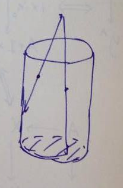
\includegraphics[scale=0.75]{assets/retract-cofibration}
	\caption{Drawing by John Ni.}
    \end{figure}
    In particular, setting $n=1$ in this example, $\{0,1\}\hookrightarrow I$ is a cofibration.
\end{example}

Here are some properties of the class of cofibrations of CGWH spaces.
\begin{itemize}
    \item It's closed under cobase change: if $A\to X$ is a cofibration, and $A\to B$ is any map,
	the pushout $B\to X\cup_A B$ is also cofibration. (Exercise!)
    \item It's closed under finite products. (This is surprising.)
    \item It's closed under composition. (Exercise!)
    \item Any cofibration is a closed inclusion\footnote{Note that the dual statement for
	fibrations would state:	any fibration $p:E\to B$ is a quotient map.
	This is definitely not true: fibrations do not have to be surjective!
	For instance, the trivial map $\emptyset\to B$ is a fibration.
	(Fibrations are surjective on path components though, because of path lifting.)}.
	\todo{This is not obvious; should we include a proof?}
\end{itemize}

\section{Homotopy fibers, the Barratt-Puppe sequence}
Yesterday, I showed this:
\begin{prop}
    If $A\to X$ is a cofibration, then for any $Y$, the map $Y^X\to Y^A$ is a fibration.
\end{prop}
We did this by reverse-engineering.
\begin{example}
    $S^{n-1}\hookrightarrow D^n$ is a cofibration.
\end{example}
Let me point out properties of cofibrations.
\begin{itemize}
    \item It's closed under cobase change. What this means is if I have a cofibration $A\to X$ and any $A\to B$, then $B\to X\cup_A B$ is a cofibration.
    \item It's closed under finite products. This is surprising.
    \item It's closed under composition.
    \item Any cofibration is a closed inclusion. This is not so obvious, so check out May's book.
\end{itemize}
By the way, the dual statement would be something like: $p:E\to B$ a quotient map? No! Fibrations don't have to be surjective at all. It is surjective on path components though, because of the path-lifting stuff. But, for example, $\emptyset\to B$ is a fibration.

Another fact on fibrations is that $X\to \ast$ is a fibration, because the dotted map can be taken to the map $(t,w)\mapsto f(w)$:
\begin{equation*}
    \xymatrix{
    W\ar[d]\ar[r]^f & X\ar[d]\\
    I\times W\ar@{-->}[ur]\ar[r] & \ast
}
\end{equation*}
Model category folks get excited about this, because this says that all objects in the model structure on topological spaces is fibrant. 
\begin{definition}
Now, the inclusion $\ast\hookrightarrow X$ is not always a cofibration (see your pset!), but if it is, say that $\ast$ is a nondegenerate basepoint in $X$.
\end{definition}
Eg if $\ast$ has a neighborhood that contracts to $\ast$ then $\ast\hookrightarrow X$ is a cofibration. If $\ast$ is a nondegenerate basepoint, then $X^A\xrightarrow{ev} X$ is a fibration where $A$ is pointed. The fiber is the space of pointed maps $A\to X$.

Because $S^{n-1}\hookrightarrow D^n$ is a cofibration, we find that $\{0,1\}\hookrightarrow I$ is a cofibration. This means that the map $Y^I\to Y\times Y$ given by $\omega\mapsto (\omega(0),\omega(1))$ is a fibration. This gets into the story of path spaces.
\subsection{''Fibrant replacements''}
Don't worry about the title of this section. If you've seen model categories, this'll make sense.
\begin{theorem}
    Any map is $\simeq$ to a fibration. What does this mean? This means that for any map $f:X\to Y$ we can find a space $T(f)$ such that:
    \begin{equation*}
	\xymatrix{
	    X\ar[dr]^{\simeq}\ar[d]_f & T(f)\ar[d]^p\\
	    & Y
	    }
    \end{equation*}
    where $p$ is a fibration and $X\xrightarrow{\simeq} T(f)$ is a homotopy equivalence.
\end{theorem}
\begin{proof}
    Consider the map $Y^I\xrightarrow{\begin{pmatrix} ev_0 \\ ev_1\end{pmatrix}}Y\times Y$. Define $T(f)$ as the pullback:
	\begin{equation*}
	    \xymatrix{
		T(f)\ar[r]\ar[d] & Y^I\ar[d]^{\begin{pmatrix}ev_0 \\ ev_1\end{pmatrix}}\\
		    X\times Y\ar[r]_{f\times 1} & Y\times Y
		}
	\end{equation*}
	In other words, $T(f)=\{(x,\omega)\in X\times Y^I|f(x) = \omega(0)\}$. Let's start checking the conditions. First of all, the map $Y^I\to Y\times Y$ is a fibration. So $T(f)\to X\times Y$ is a fibration. Since $X\times Y\to Y$ is a fibration, we can consider the composite $T(f)\to X\times Y\to Y$, which is now a fibration. On elements, $T(f)\to Y$ sends $(x,\omega)\to \omega(1)$.

	To get a map $X\to T(f)$, I need to give maps $X\to X\times Y$ and $X\to Y^I$ that have compatible images in $Y\times Y$. Define $X\to X\times Y$ as $X\xrightarrow{\begin{pmatrix} 1 \\ f\end{pmatrix}}X\times Y$, and define $X\to Y^I$ as the map sending $x$ to the constant loop at $f(x)$. Clearly both composite $X\to X\times Y\\to Y\times Y$ and $X\to Y^I\to Y\times Y$ are the same, so we have a map $X\to T(f)$.

	    Is it true that the composite $X\to T(f)\xrightarrow{p} Y$ is our original map? Yes! So we only have to check that $X\to T(f)$ is a homotopy equivalence. Let me begin by constructing a homotopy inverse. I.e., a map $T(f)\to X$. We can define a map $T(f)\to X$ via $T(f)\to X\times Y\xrightarrow{pr_1} X$. Clearly the composite $X\to T(f)\to X\times Y\to X$ is the identity. This means we need to study $T(f)\to X\to T(f)$. This composite sends $(x,\omega)\mapsto x\mapsto (x,c_{f(x)})$ where $c_{f(x)}$ is the constant path at $x$. I need a homotopy between this map and the identity on $T(f)$.

	    This is what I call the spaghetti move. We know that there's no constraint on $\omega(1)$, so I can just suck it back in to get the constant loop. I guess I can define $\omega_s(t) = \omega(st)$. At $s=1$ I have $\omega$ and when $s=0$ I have $c_{f(x)} = c_{\omega(0)}$. Thus, define $I\times T(f)\to T(f)$ via $(s,(x,\omega))\mapsto (x,\omega_s)$.

	    If you want to work through the diagram, this is how it looks.
	    \begin{equation*}
		\xymatrix{
		    X\ar@{-->}[dr]\ar[drr]^{x\mapsto c_{f(x)}}\ar[ddr]_{\begin{pmatrix}1 \\ f\end{pmatrix}} & & \\
			& T(f)\ar[d]\ar[r]\ar[dr] & Y^I\ar[d]^{\begin{pmatrix}ev_0 \\ ev_1\end{pmatrix}}\\
			    X & X\times Y\ar[l]^{pr_1}\ar[d]^{pr_2}\ar[r] & Y\times Y\\
		    & Y
		    }
	    \end{equation*}
\end{proof}
Here's a really stupid example. 
\begin{example}[Path-loop fibration]
Suppose $X=\ast$. What is $T(f)$? Well it's just paths $\omega(0)$ in $Y$ such that $\omega(0)=\ast$. I.e., $T(f) = Y^I_\ast$. This is also called the path space of $Y$, denoted $P(Y,\ast)$. It's contractible by the spaghetti move. What it's fiber? The map $PY\to Y$ sends $\omega\mapsto \omega(1)$. So the fiber is the points that begin at $\ast$ and end at $\ast$. The fiber of $PY\to Y$ is denoted $\Omega Y$, which is the space of loops at $\ast$. This is called the path loop fibration. 
\end{example}
\subsection{Homotopy fibers over $\ast$}
The ordinary fiber is the pullback
\begin{equation*}
    \xymatrix{
	f^{-1}(\ast)\ar[r]\ar[d] & X\ar[d]^f\\
	\ast\ar[r] & Y
    }
\end{equation*}
\begin{definition}[Homotopy fiber]
    The homotopy fiber is the pullback:
    \begin{equation*}
	\xymatrix{
	    F(f,\ast)\ar[r]\ar[d] & T(f)\ar[r]\ar[d]^p & X\ar[dl]^f\\
	    \ast \ar[r] & Y &
	    }
    \end{equation*}
\end{definition}
As a set it's $F(f,\ast) = \{(x,\omega)\in X\times Y^I| f(x) = \omega(0), \omega(1) = \ast\}$. The ordinary fiber and the homotopy fiber are definitely not generally the same. If $W\to X\to Y$ is nullhomotopic, then it factors through $F(f,\ast)$, i.e., the composite factors as $W\to F(f,\ast)\to X\to Y$.
\begin{prop}
    Suppose $p:X\to Y$ is a fibration. Let $\ast\in Y$. Then $p^{-1}(\ast)\to F(p,\ast)$ is a homotopy equivalence.
\end{prop}
I'm not going to prove that, but you will for homework.

A different way to construct the homotopy fiber is to replace $f:X\to Y$ by a fibration. But what if I replace $\ast\to Y$ by a fibration? Namely, we now have:
\begin{equation*}
    \xymatrix{
	??\ar[r]\ar[d] & P(Y,\ast)\ar[r]^{\simeq} & \ast\ar[dl]\\
	X\ar[r] & Y & 
    }
\end{equation*}
This space $??$ consists of $(x,\omega)\in X\times Y^I$ such that $\omega(0) = \ast$ and $\omega(1) = f(x)$. Now, $F(f,\ast) = \{(x,\omega):\omega(0) = f(x), \omega(1) = \ast\}$. So $??$ is homeomorphic to $F(f,\ast)$ by reversing directions of paths. There's two ways you can produce a homotopy fiber, and all of these are homeomorphic. You could also replace both of these maps $f$ and $\ast\to Y$ by a fibration, and you'll get something that's also homeomorphic. Note that when I say $F(f,\ast)$, I'll mean $??$.

Here's what you'll prove for homework.
\begin{theorem}
    Suppose you have two fibrations $p$ and $p^\prime$ such that the following diagram commutes, where $f$ is a homotopy equivalence.
    \begin{equation*}
	\xymatrix{
	    E\ar[r]^p\ar[dr]^p & E^\prime\ar[d]^{p^\prime}\\
	    & B
	    }
    \end{equation*}
    Then $f$ is a fiber homotopy equivalence. That means that it's a homotopy equivalence in $\Top_{/B}$. What this means is that there is a map $g:E^\prime\to E$ over $B$ compatible with the fibrations and homotopies $I\times E\to E$ over $B$ and $I\times E^\prime\to E^\prime$ over $B$. I.e., the following three diagrams commute:
    \begin{equation*}
	\xymatrix{
	    E^\prime\ar[r]^g\ar[dr]^{p^\prime} & E\ar[d]^p\\
	    & B
	    }
    \end{equation*}
    and 
    \begin{equation*}
	\xymatrix{
	    I\times E\ar[r]^{1\sim gf}\ar[dr] & E\ar[d]^p\\
	    & B
	    }
    \end{equation*}
    and
    \begin{equation*}
	\xymatrix{
	    I\times E^\prime\ar[r]^{1\sim fg}\ar[dr] & E^\prime\ar[d]^{p^\prime}\\
	    & B
	    }
    \end{equation*}
\end{theorem}
So we find that for all $b$, $p^{-1}(b)\xrightarrow{\simeq} (p^\prime)^{-1}(b)$. So in particular, the fiber $F(f,\ast)$, i.e., the homotopy fiber, of $T(f)\to B$ and the fiber $f^{-1}(\ast)$ of $f:E\to B$ are homotopy equivalent if $f$ is a fibration.

\section{Barratt-Puppe sequence, $\pi_\ast$}
Hood's office hours are from 12 to 1:30 on Mondays in 2-390. Mine are from 4-5 on Tuesday in 2-478. Hood's graded the homework already.
\subsection{Fiber sequences}
Recall we have a pullback diagram:
\begin{equation*}
    \xymatrix{
	& F(f,\ast)\ar[r]\ar[d]^p & PY\ar[d]^p\ar[dr]^{\simeq} & \\
	f^{-1}(\ast)\ar[ur]\ar[r] & X\ar[r]_f & Y & \ast\ar[l]
    }
\end{equation*}
The homotopy fiber $F(f,\ast)$ thus has elements $\{(x,\sigma)\in X\times PY| f(x) = \sigma(1)\}$. We also have the ordinary fiber $f^{-1}(\ast)$. If $f$ is a fibration, the canonical map $f^{-1}(\ast)\to F(f,\ast)$ sending $x\mapsto(x,c_{f(x)})$ is a homotopy equivalence.
\begin{remark}
Consider a pointed map\footnote{Some people say ``based maps'', but it sounds like chemistry ... or evil, so I can't bring myself to say it} $f:X\to Y$, i.e., $f(\ast) = \ast$. Then I'll write $Ff$ for $F(f,\ast)$.
\end{remark}
Ok, what's the fiber of $p:Ff\to X$? The fiber over the basepoint in $X$ is precisely the space of loops in $Y$! I.e., $p^{-1}(\ast_X) = \Omega Y$, which is the space of loops in $Y$ based at $\ast_Y$. Note that this is also the homotopy fiber because $p$ is a fibration (fibrations are closed under pullbacks). So the diagram we now have is:
\begin{equation*}
\xymatrix{\\
    & \Omega Y=p^{-1}(\ast)\ar[d] & & &\\
    & F(f,\ast)\ar[r]\ar[d]^p & PY\ar[d]^p\ar[dr]^{\simeq} & \\
    f^{-1}(\ast)\ar[ur]\ar[r] & X\ar[r]_f & Y & \ast\ar[l]
}
\end{equation*}
The composite $Ff\to X\to Y$ sends $(x,\omega)\mapsto f(x)$. This is a pointed map, but not equal to the constant map. What does this even mean? Like, what is the basepoint we're choosing for $Ff$? Well, choose the basepoint to be the image of the basepoint in $f^{-1}(\ast)$ under $f^{-1}(\ast)\hookrightarrow Ff$.

We also have a (pointed!) homotopy between $Ff\to X\to Y$ and the constant map, eg via $h:Ff\times I\to Y$ defined by $h(t,(x,\omega)) = \omega(t)$. We say that the composite is \emph{nullhomotopic}. In fact, suppose $W\to X\to Y$ is nullhomotopic, with a chosen nullhomotopy -- this is the same as a map $W\to Ff$. This is a question on your homework.

Let's write $[W,X]_\ast = \pi_0(X^W_\ast)$, i.e., the pointed homotopy classes of maps $W\to X$. This is a pointed set, whose basepoint is the constant map. Ok, I can consider $[W,Ff]_\ast\to [W,X]_\ast\to [W,Y]_\ast$. This composite is nullhomotopic. But I want to say that this sequence is exact. What that means is here (because we just have pointed sets). So the preimage of the basepoint in $[W,Y]_\ast$ equals the image of $[W,Ff]_\ast\to [W,X]_\ast$. This is exactly what I said before, about nullhomotopies $W\to X\to Y$ as maps $W\to Ff$. We say that $Ff\to X\xrightarrow{f}Y$ is a \emph{fiber sequence}.

\subsection{Iterating fiber sequences}
I have $Ff\xrightarrow{p} X\xrightarrow{f} Y$. The strict fiber is $\Omega Y$, but the homotopy fiber is $Fp$. These are homotopy equivalent because $p$ is a fibration. Denote the map $i:\Omega Y\to Ff$. This sits inside:
\begin{equation*}
    \xymatrix{
	\cdots\ar[r] & Fp_3 \ar[r] & Fp_2\ar[r] & Fp_1\ar[r]^{p_2} & Ff\ar[r]^{p_1} & X\ar[r]^{f} & Y\\
	& \Omega Fp_0\ar[u]_{\simeq}\ar[ur]|{i(p_2)}\ar@{-->}[r] & \Omega X\ar@{-->}[r]\ar[u]_{\simeq}\ar[ur]|{i(p_1)} & \Omega Y\ar[u]_\simeq \ar[ur]|{i(p_0)} & &
    }
\end{equation*}
All the $p_i$s are fibrations (think about why). The dotted maps seem to be missing; I can fill them in up to homotopy, and there's one map I can think of putting there: $\Omega X\xrightarrow{\Omega f}\Omega Y$. But \emph{that's the wrong map}! The right map is $\Omega X\xrightarrow{\overline{\Omega f}}\Omega Y$ (see below for explanation). Here's a lemma.
\begin{lemma}
    The following diagram commutes to homotopy:
    \begin{equation*}
	\xymatrix{
	    & Fp\\
	    \Omega X\ar[r]_{\overline{\Omega f}}\ar[ur]^{i(p)} & \Omega Y\ar[u]
	    }
    \end{equation*}
    where $\overline{\Omega f}$ is the diagonal in:
    \begin{equation*}
	\xymatrix{
	    \Omega X\ar[r]^{-}\ar[dr]|{\Omega f} \ar[d]_{\Omega f} & \Omega X\ar[d]^{\Omega f}\\
	    \Omega Y\ar[r]_{-} & \Omega Y
	    }
    \end{equation*}
    where $-:\Omega X\to \Omega X$ sends $\omega\mapsto\overline{\omega}$.
\end{lemma}
\begin{proof}
    There is a beautiful proof of this. But it's in pictures, and I can't type it. The main point is that the proof wouldn't work unless you moved backwards. See this image:
\begin{figure}[H]
\centering
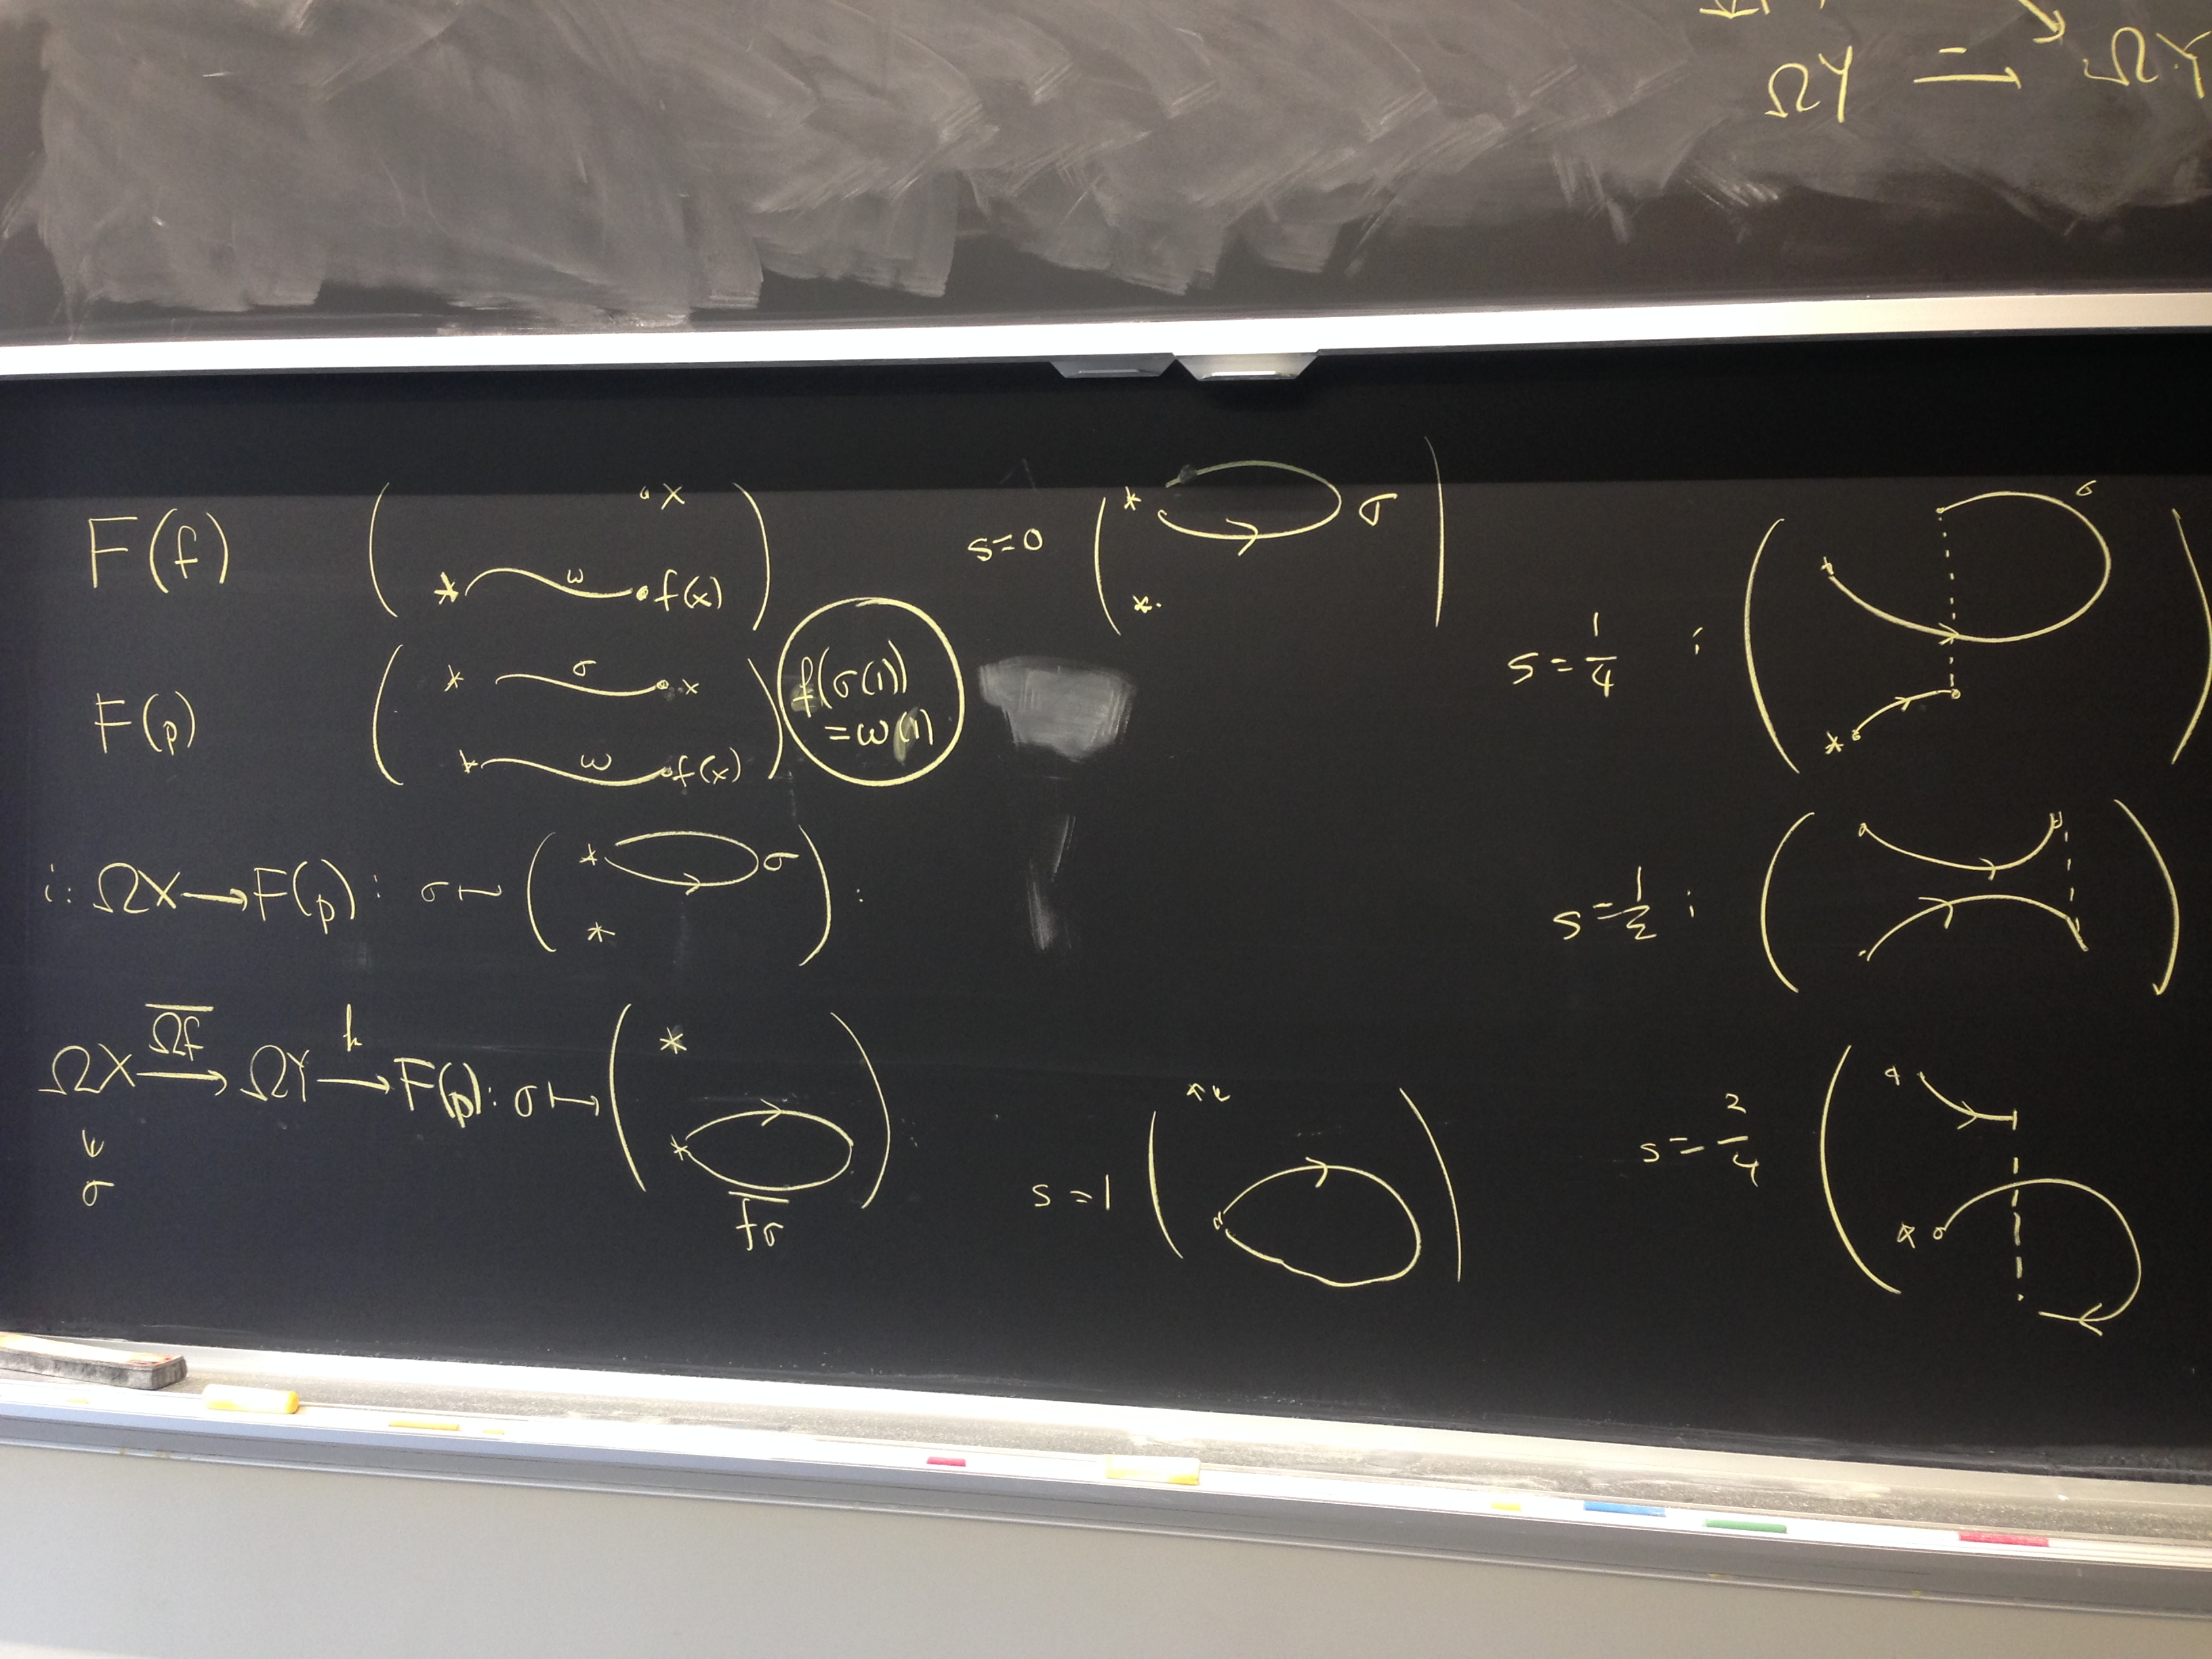
\includegraphics[width=\textwidth]{assets/barratt-puppe}
\caption{A proof of this lemma.}
\end{figure}
\end{proof}
\begin{lemma}
    The following diagram commutes:
    \begin{equation*}
	\xymatrix{
	    & F(\overline{\Omega p_0})\ar@{=}[dd]\ar[dr] & \\
	    \Omega^2 Y\ar[ur]^{i(\Omega p_0)}\ar[dr]_{\overline{\Omega i(p_0)}} & & \Omega X\\
	    & \Omega Fp_0\ar[ur]_{\overline{\Omega p_1}} & 
	    }
    \end{equation*}
\end{lemma}
What is the map $F\overline{\Omega p_0}\to \Omega X$?? We spent some time figuring this out. But you can now apply $[W,-]_\ast$ to the following diagram to get a long exact sequence:
\begin{equation*}
    \xymatrix{
	\cdots\ar[r] & Fp_4\ar[r] & Fp_3 \ar[r] & Fp_2\ar[r] & Fp_1\ar[r]^{p_2} & Ff\ar[r]^{p_1} & X\ar[r]^{f} & Y\\
    \cdots\ar[r] & \Omega Fp_1\ar[r]|{\overline{\Omega p_2}}\ar[u]_{\simeq} & \Omega Fp_0\ar[u]_{\simeq}\ar[ur]|{i(p_2)}\ar[r]|{\overline{\Omega p}} & \Omega X\ar[r]|{\overline{\Omega f}}\ar[u]_{\simeq}\ar[ur]|{i(p_1)} & \Omega Y\ar[u]_\simeq \ar[ur]|{i(p_0)} & &\\
	\Omega^2 X\ar[u]_{\simeq}\ar[r]_{\Omega f} & \Omega Y\ar[u]_{\simeq}\ar[ur]_{\overline{\Omega i(p_0)}} & & &
    }
\end{equation*}

For example, $S^0=\{\pm 1\}$. We get terms like $\pi_0(\Omega^n X)$, because $[S^0,X] = \pi_0 X$. What is $\pi_0(\Omega^n X)$? This is $[S^0,\Omega^n X]_\ast$. Is it clear to you that this is $[S^n,X]_\ast$?

Ok, well, $\Omega^2 X = (\Omega X)^{S^1}$. Because $(S^1)^{\wedge n} = S^n$. So we find that $(\Omega X)^{S^1} = (X^{S^1}_\ast)^{S^1}_\ast = X_\ast^{S^1\wedge S^1} = X_\ast^{S^2}$.

Well, $\Omega X$ is a homotopy group by concatenation. It's a group, but where the axioms hold up to homotopy. It's a group in the homotopy category. Therefore, $\pi_0 \Omega X$ is a group! It's exactly $\pi_1 X$, which you know to be a group. And then, there's this other thing that happens.

You can think of $\pi_n(X) = [S^n,X]_\ast$ as $[(D^n,S^{n-1}),(X,\ast)] = [(I^n,\partial I^n),(X,\ast)]$. If I take $n=2$, for example, how do I take the product of $\alpha,\beta\in \pi_2(X)$? You just literally put them together (when you think of $\pi_2(X) = [(I^2,\partial I^2),(X,\ast)]$. You can play this game; up to homotopy, you can shrink $\alpha$ and $\beta$ to make them as small I want, and then reverse their position and expand them again\footnote{This probably makes no sense without a picture}\todo{Add a picture}. Thus $\pi_2(X)$ is an abelian group.

Thus, when you apply $\pi_0$ to our sequence $\cdots\to\Omega^2 X\to\Omega^2 Y\to \Omega Fp_0\to \Omega X\to \Omega Y\to Fp_0\to \Omega X\to \Omega Y$, you get an exact sequence (of groups when the homotopy groups are $>0$, and of pointed sets when you have $\pi_0$):
$$\cdots\to \pi_2 X\to \pi_2 Y\to \pi_1 Ff\to \pi_1 X\to\pi_1 Y\to\pi_0 Ff\to\pi_0 X\to \pi_0 X$$

\section{Relative homotopy groups}
%Pset 2 has question 8; there's still one more to go. Hood has office hours today 12 -- 1 in 2-390, and I have office hours today tomorrow 4-5 in 2-478.
\subsection{Spheres and homotopy groups}
The functor $\Omega$ (sending a space to its based loop space) admits a left adjoint.
To see this, recall that $\Omega X = X^{S^1}_\ast$, so that
$$\Top_\ast(W,\Omega X) = \Top_\ast(S^1\wedge W,X).$$
\begin{definition}
    The \emph{reduced suspension} $\Sigma W$ is $S^1\wedge W$.
\end{definition}
If $A\subseteq X$, then
$$X/A\wedge Y/B = (X\times Y)/((A\times Y)\cup_{A\times B}(X\times B)).$$
Since $S^1 = I/\partial I$, this tells us that $\Sigma X = S^1\wedge X$ can be identified with
$I\times X/(\partial I \times X\cup I\times \ast)$: in other words, we collapse the top and bottom of a cylinder to a point,
as well as the line along a basepoint.

The same argument says that $\Sigma^n X$ (defined inductively as $\Sigma(\Sigma^{n-1} X)$)
is the left adjoint of the $n$-fold loop space functor $X\mapsto \Omega^n X$.
In other words, $\Sigma^n X = (S^1)^{\wedge n}\wedge X$.
We claim that $S^1\wedge S^n \simeq S^{n+1}$.
To see this, note that
$$S^1\wedge S^n = I/\partial I\wedge I^n\wedge \partial I^n = (I\times I^n)/(\partial I\times I^n\cup I\times \partial I^n).$$
The denominator is exactly $\partial I^{n+1}$, so $S^1\wedge S^n\simeq S^{n+k}$.
It's now easy to see that $S^k\wedge S^n\simeq S^{k+n}$.
\begin{definition}
    The \emph{$n$th homotopy group} of $X$ is $\pi_n X = \pi_0(\Omega^n X)$.
\end{definition}
This is, as we noted in the previous section, $[S^0,\Omega^n X]_\ast = [S^n, X]_\ast = [(I^n,\partial I^n),(X,\ast)]$.

\subsection{The homotopy category}
Define the \emph{homotopy category of spaces} $\Ho(\Top)$ to be the category
whose objects are spaces, and whose hom-sets are given by taking $\pi_0$ of the mapping space.
To check that this is indeed a category, we need to check that if $f_0,f_1:X\to Y$ and $g:Y\to Z$, then $gf_0\simeq gf_1$ ---
but this is clear.
Similarly, we'd need to check that $f_0h\simeq f_1h$ for any $h:W\to X$.
We can also think about the homotopy category of pointed spaces (and pointed homotopies) $\Ho(\Top_\ast)$; this is the category
we have been spending most of our time in.
Both $\Ho(\Top)$ and $\Ho(\Top_\ast)$ have products and coproducts, but very few other limits or colimits.
From a category-theoretic standnpoint, these are absolutely terrible.

Let $W$ be a pointed space.
We would like the assignment $X\mapsto X^W_\ast$ to be a homotopy functor.
It clearly defines a functor $\Top_\ast\to\Top_\ast$, so this desire is equivalent to providing a dotted arrow in the
following diagram:
\begin{equation*}
    \xymatrix{
	\Top_\ast\ar[d]\ar[r]^{X\mapsto X^W_\ast} & \Top_\ast\ar[d]\\
	\Ho(\Top_\ast)\ar@{-->}[r] & \Ho(\Top_\ast).
    }
\end{equation*}
Before we can prove this, we will check that a homotopy $f_0\sim f_1:X\to Y$ is the same as a map $I_+\wedge X\to Y$.
There is a nullhomotopy if the basepoint of $I$ is one of the endpoints, so a homotopy is the same as a map
$I\times X/I\times\ast \to Y$. The source is just $I_+\wedge X$, as desired.

A homotopy $f_0 \simeq f_1:X\to Y$ begets a map $(I_+\wedge X)^W\to Y^W_\ast$.
For the assignment $X\mapsto X^W_\ast$ to be a homotopy functor, we need a natural transformation $I_+\wedge X^W_\ast\to Y^W_\ast$, so this map is not quite what's necessary.
Instead, we can attempt to construct a map $I_+\wedge X^W_\ast\to (I_+\wedge X)^W_\ast$.

We can construct a general map $A\wedge X^W_\ast\to (A\wedge X)^W_\ast$: 
there is a map $A\wedge X^W_\ast\to A^W_\ast\wedge X^W_\ast$, given by sending $a\mapsto c_a$;
then the exponential law gives a homotopy $A^W_\ast\wedge X^W_\ast\to (A\wedge X)^W_\ast$.
This, in turn, gives a map $I_+\wedge X^W_\ast\to (I_+\wedge X)^W_\ast\to Y^W_\ast$,
thus making $X\mapsto X^W_\ast$ a homotopy functor.

Motivated by our discussion of homotopy fibers, we can study composites which ``behave'' like short exact sequences.
\begin{definition}
    A \emph{fiber sequence} in $\Ho(\Top_\ast)$ is a composite $X\to Y\to Z$ that is
    isomorphic, in $\Ho(\Top_\ast)$, to some composite $Ff\xrightarrow{p} E\xrightarrow{f}B$;
    in other words, there exist (possibly zig-zags of) maps that are homotopy equivalences, that make the following
    diagram commute:
    \begin{equation*}
	\xymatrix{
	    X\ar[r]\ar[d] & Y\ar[r]\ar[d] & Z\ar[d]\\
	    Ff\ar[r]_p & E\ar[r]_f & B.
	    }
    \end{equation*}
\end{definition}
Let us remark here that if $A^\prime \xar{\sim} A$ is a homotopy equivalence, and $A\to B \to C$ is a fiber sequence, so
is the composite $A^\prime\xar{\sim} A \to B\to C$.

\begin{exercise}\label{loopslimit}
    Prove the following statements.
    \begin{itemize}
	\item $\Omega$ takes fiber sequences to fiber sequences.
	\item $\Omega Ff\simeq F\Omega f$. Check this!
    \end{itemize}
\end{exercise}

We've seen examples of fiber sequences in our elaborate study of the Barratt-Puppe sequence.
\begin{example}
Recall our diagram:
\begin{equation*}
    \xymatrix{
	\cdots\ar[r] & Fp_4\ar[r] & Fp_3 \ar[r] & Fp_2\ar[r] & Fp_1\ar[r]^{p_2} & Ff\ar[r]^{p_1} & X\ar[r]^{f} & Y\\
    \cdots\ar[r] & \Omega Fp_1\ar[r]|{\overline{\Omega p_2}}\ar[u]_{\simeq} & \Omega Ff\ar[u]_{\simeq}\ar[ur]|{i(p_2)}\ar[r]|{\overline{\Omega p}} & \Omega X\ar[r]|{\overline{\Omega f}}\ar[u]_{\simeq}\ar[ur]|{i(p_1)} & \Omega Y\ar[u]_\simeq \ar[ur]|{i(f)} & &\\
	\Omega^2 X\ar[u]_{\simeq}\ar[r]_{\Omega f} & \Omega Y\ar[u]_{\simeq}\ar[ur]_{\overline{\Omega i(f)}} & & &
    }
\end{equation*}
The composite $Ff\to X\xar{f} Y$ is canonically a fiber sequence.
The above diagram shows that $\Omega Y\to F\xrightarrow{p}X$ is another fiber sequence: it is isomorphic to
$Fp\to F\to X$ in $\Ho(\Top_\ast)$.
Similarly, the composite $\Omega X\xrightarrow{\overline{\Omega f}}\Omega Y\to F$ is another fiber sequence;
this implies that $\Omega X\xrightarrow{\Omega f}\Omega Y\to F$ is also an example of a fiber sequence
(because these two fiber sequences differ by an automorphism of $\Omega X$)

Applying $\Omega$ again, we get $\Omega F\xrightarrow{\Omega p} \Omega X\xrightarrow{\Omega f} \Omega Y$.
Since this is a looping of a fiber sequence, and taking loops takes fiber sequences to fiber sequences (Exercise \ref{loopslimit}), this is another fiber sequence. 
Looping again gives another fiber sequence $\Omega^2 Y\xrightarrow{\Omega i} \Omega F\xrightarrow{\Omega p}\Omega X$.
(For the category-theoretically--minded folks, this is an unstable version of a triangulated category.)
\end{example}

\subsection{The long exact sequence of a fiber sequence}
As discussed at the end of \S \ref{secbarrattpuppe}, applying $\pi_0 = [S^0,-]_\ast$ to the
Barratt-Puppe sequence associated to a map $f:X\to Y$ gives a long exact sequence:
\begin{equation*}
    \xymatrix{
	& \cdots\ar[r] & \pi_2 Y\ar[dll]\\
	\pi_1 F\ar[r] & \pi_1 X\ar[r] & \pi_1 Y\ar[dll]\\
	\pi_0 F\ar[r] & \pi_0 X. & 
    }
\end{equation*}
of pointed sets.
The space $\Omega^2 X$ is an \emph{abelian} group object in $\Ho(\Top)$
(in other words, the multiplication on $\Omega^2 X$ is commutative up to homotopy).
This implies $\pi_1(X)$ is a group, and that $\pi_k(X)$ is abelian for $k\geq 2$;
hence, in our diagram above, all maps (except on $\pi_0$) are group homomorphisms.

Consider the case when $X\to Y$ is the inclusion $i:A\hookrightarrow X$ of a subspace.
In this case,
$$Fi=\{(a,\omega)\in A\times X^I_\ast|\omega(1) = a\};$$
this is just the collection of all paths that begin at $\ast\in A$ and end in $A$.
This motivates the definition of \emph{relative homotopy groups}:
\begin{definition}
    Define: 
    $$\pi_n(X,A,\ast) = \pi_n(X,A) := \pi_{n-1}Fi = [(I^n,\partial I^n,(\partial I^n\times I)\cup (I^{n-1}\times 0)),(X,A,\ast)].$$
\end{definition}
We have a sequence of inclusions
$$\partial I^n\times I\cup I^{n-1}\times 0 \subset \partial I^n \subset I^n.$$
One can check that
$$\pi_{n-1}Fi = [(I^n,\partial I^n,(\partial I^n\times I)\cup (I^{n-1}\times 0)),(X,A,\ast)].$$
This gives a long exact sequence on homotopy, analogous to the long exact sequence in relative homology:
\begin{equation*}
    \xymatrix{
	& \cdots\ar[r] & \pi_2 (X,a)\ar[dll]\\
	\pi_1 A\ar[r] & \pi_1 X\ar[r] & \pi_1 (X,A)\ar[dll]\\
	\pi_0 A\ar[r] & \pi_0 X. & 
    }
\end{equation*}

\section{Action of $\pi_1$, simple spaces, and the Hurewicz theorem}
In the previous section, we constructed a long exact sequence of homotopy groups:
\begin{equation*}
    \xymatrix{
	& \cdots\ar[r] & \pi_2 (X,A)\ar[dll]\\
	\pi_1 A\ar[r] & \pi_1 X\ar[r] & \pi_1 (X,A)\ar[dll]\\
	\pi_0 A\ar[r] & \pi_0 X, & 
    }
\end{equation*}
which looks suspiciously similar to the long exact sequence in homology.
The goal of this section is to describe a relationship between homotopy groups and homology groups.

Before we proceed, we will need the following lemma.
\begin{lemma}[Excision]
    If $A\subseteq X$ is a cofibration, there is an isomorphism
    $$H_\ast(X,A)\xrightarrow{\simeq}\widetilde{H}_\ast(X/A).$$
    Under this hypothesis,
    $$X/A\simeq\text{Mapping cone of }i:A\to X;$$
    here, the mapping cone is the homotopy pushout in the following diagram:
    \begin{equation*}
	\xymatrix{
	    A\ar[r]^i\ar[d]^{in_1} & X\ar[d]\\
	    CA\ar[r] & X\cup_A CA,
	    }
    \end{equation*}
    where $CA$ is the cone on $A$, defined by
    $$CA = A\times I/A\times 0.$$
\end{lemma}
This lemma is dual to the statement that the homotopy fiber is homotopy equivalent to the strict fiber for fibrations.

Unfortunately, $\pi_\ast(X,A)$ is definitely not $\pi_\ast(X/A)$!
For instance, there is a cofibration sequence
$$S^1\to D^2\to S^2.$$
We know that $\pi_\ast S^1$ is just $\Z$ in dimension $1$, and is zero in other dimensions.
On the other hand, we do not, and probably will never, know the homotopy groups of $S^2$.
(A theorem of Edgar Brown \todo{find a citation} says that these groups are computable, but this is super-exponential.)
%\begin{theorem}[Now]
%    If $X$ is a simply connected finite complex, and $X\not\simeq \ast$, then we do not know $\pi_\ast(X)$. And we'll probably never be able to know them.
%\end{theorem}
%These groups \emph{are} computable (a theorem by Edgar Brown), but it's super-exponential. This is discouraging. We'll never know what, eg., $\pi_{10000}(S^2)$ is.

%Anyway, I said there was $\partial:\pi_n(X,A,\ast)\to \pi_{n-1}(A,\ast)$. How does this look? Well you just look at the restriction of $I^n\to X$ to $1\times I^{n-1}\to A$. And the composite $\pi_n(X,A,\ast)\xrightarrow{\partial}\pi_{n-1}(A,\ast)\to \pi_{n-1}(X,\ast)$ is trivial by definition!
\subsection{$\pi_1$-action}
There is more structure in the long exact sequence in homotopy groups that we constructed last time, coming from an action
of $\pi_1(X)$.
There is an action of $\pi_1(X)$ on $\pi_n(X)$: if $x,y$ are points in $X$, and $\omega:I\to X$ is a path with $\omega(0) = x$ and $\omega(1) = y$, we have a map $f_\omega:\pi_n(X,x)\to \pi_n(X,y)$;
this, in particular, implies that $\pi_1(X,\ast)$ acts on $\pi_n(X,\ast)$.
When $n=1$, the action $\pi_1(X)$ on itself is by conjugation.

In fact, one can also see that $\pi_1(A)$ acts on $\pi_n(X,A,\ast)$.
It follows (by construction) that all maps in the long exact sequence of Equation \eqref{lexseqhomotopy} are equivariant for
this action of $\pi_1(A)$.
Moreover:
\begin{prop}[Peiffer identity]
    Let $\alpha,\beta\in \pi_2(X,A)$. Then $(\partial \alpha)\cdot\beta = \alpha\beta\alpha^{-1}$.
\end{prop}
%For example, if $j:\pi_2(X)\to \pi_2(X,A)$, and $\alpha = j(\gamma)$, $\partial\alpha = 1$: $\img(k)\subseteq\coker \pi_2(X,A)$. (I did not follow this)

\begin{definition}
    A topological space $X$ is said to be \emph{simply connected} if it is path connected, and $\pi_1(X,\ast) = 1$.
\end{definition}
Let $p:E\to B$ be a covering space with $E$ and $B$ connected.
Then, the fibers are discrete, hence do not have any higher homotopy.
Using the long exact sequence in homotopy groups, we learn that $\pi_n(E)\to \pi_n(B)$ is an isomorphism for $n>1$,
and that $\pi_1(E)$ is a subgroup of $\pi_1(B)$ that classifies the covering space.
In general, we know from Exercise \ref{simplequotient} that $\Omega B$ acts on the homotopy fiber $Fp$.
Since $Ff$ is discrete, this action factors through $\pi_0(\Omega B)\simeq \pi_1(B)$.

%In particular, $\pi_q(S^n)\simeq \pi_q(\RP^n)$ for $q>1$. Of course, $\pi_1(\RP^n)\simeq \Z/2\Z$. This creates a ton of homology in $\RP^n$ that's not present in the homology of $S^n$. Here's a piece of language.
\begin{definition}
    A space $X$ is said to be \emph{$n$-connected} if $\pi_i(X) = 0$ for $i\leq n$.
\end{definition}
Note that this is a well-defined condition, although we did not specify the basepoint: $0$-connected implies path connected.
Suppose $E\to B$ is a covering space, with the total space $E$ being $n$-connected.
Then, Hopf showed that the group $\pi_1(B)$ determines the homology $H_i(B)$ in dimensions $i<n$.
%in particular, $H_i(B) = H_i(\pi_1(B))$, which is the group homology. This is due to Heinz Hopf.

Sometimes, there are interesting spaces which are not simply connected, for which the $\pi_1$-action is nontrivial.
\begin{example}
    Consider the space $S^1\vee S^2$.
    The universal cover is just $\RR$, with a $2$-sphere $S^2$ stuck on at every integer point.
    This space is simply connected, so the Hurewicz theorem says that $\pi_2(E)\simeq H_2(E)$.
    Since the real line is contractible, we can collapse it to a point: this gives a countable bouquet of $2$-spheres.
    As a consequence, $\pi_2(E)\simeq H_2(E) = \bigoplus_{i=0}^\infty \Z$.

    There is an action of $\pi_1(S^1\vee S^2)$ on $E$: the action does is shift the $2$-spheres on the integer points of $\RR$ (on $E$) to the right by $1$ (note that $\pi_1(S^1\vee S^2) = \Z$).
    This tells us that $\pi_2(E) \simeq \Z[\pi_1(B)]$ as a $\Z[\pi_1(B)]$-module; this is the same action of $\pi_1(E)$ on
    $\pi_2(E)$.
    We should be horrified: $S^1\vee S^2$ is a very simple $3$-complex, but its homotopy is huge!
\end{example}
Simply-connectedness can sometimes be a restrictive condition; instead, to simplify the long exact sequence, we define:
\begin{definition}
    A topological space $X$ is said to be \emph{simple} if it is path-connected, and
    $\pi_1(X)$ acts trivially on $\pi_n(X)$ for $n\geq 1$.
\end{definition}
Note, in particular, that $\pi_1(X)$ is abelian for a simple space.

Being simple is independent of the choice of basepoint. If $\omega:x\mapsto x^\prime$ is a path in $X$,
then $\omega_\sharp:\pi_n(X,x)\to \pi_n(X,x^\prime)$ is a group isomorphism.
There is a (trivial) action of $\pi_1(X,x)$ on $\pi_n(X,x)$, and another (potentially nontrivial)
action of $\pi_1(X,x^\prime)$ on $\pi_n(X,x^\prime)$.
Both actions are compatible: hence, if $\pi_1(X,x)$ acts trivially, so does $\pi_1(X,x^\prime)$.

If $X$ is path-connected, there is a map $\pi_n(X,\ast)\to [S^n,X]$.
It is clear that this map is surjective,
%because I can always choose a basepoint in $X$ as the image of a basepoint in $S^n$.
so one might expect a factorization:
\begin{equation*}
    \xymatrix{
	\pi_n(X,\ast)\ar@{->>}[r]\ar[dr] & [S^n,X]\\
	& \pi_1(X,\ast)\backslash \pi_n(X,\ast)\ar[u]
	}
\end{equation*}
\begin{exercise}\label{simplequotient}
    %Exercises 7 and 9 of pset 2
    Prove that $\pi_1(X,\ast)\backslash \pi_n(X,\ast) \simeq [S^n, X]$.
    To do this, work through the following exercises.
    
    Let $f:X\to Y$ be a map of spaces, and let $\ast\in Y$ be a fixed basepoint of $Y$.
    Denote by $Ff$ the homotopy fiber of $f$; this admits a natural fibration $p:Ff \to X$, given by $(x,\sigma)\mapsto x$.
    If $\Omega Y$ denotes the (based) loop space of $Y$, we get an action $\Omega Y \times Ff \to Ff$, given by
    $$(\omega,(x,\sigma)) \mapsto (x,\sigma\cdot\omega),$$
    where $\sigma\cdot\omega$ is the concatenation of $\sigma$ and $\omega$, defined, as usual, by
    $$
    \sigma\cdot\omega(t) = \begin{cases}
	\omega(2t) & 0\leq t\leq 1/2\\
	\sigma(2t-1) & 1/2\leq t\leq 1.
    \end{cases}
    $$
    (Note that when $X$ is the point, this defines a ``multiplication'' $\Omega Y \times \Omega Y \to \Omega Y$; this is 
    associative and unital up to homotopy.)
    On connected components, we therefore get an action of $\pi_0\Omega Y \simeq \pi_1 Y$ on $\pi_0 Ff$.

    There is a canonical map
    $$Ff \times \Omega Y \to Ff\times_X Ff,$$
    given by $((x,\sigma),\omega) \mapsto ((x,\sigma),(x,\sigma)\cdot\omega)$.
    Prove that this map is a homotopy equivalence (so that the action of $\Omega Y$ on $Ff$ is ``free''), and conclude that
    two elements in $\pi_0 Ff$ map to the same element of $\pi_0 X$ if and only if they are in the same orbit under the action
    of $\pi_1 Y$.

    Let $X$ be path connected, with basepoint $\ast\in X$.
    Conclude that $\pi_1(X,\ast)\backslash \pi_n(X,\ast) \simeq [S^n,X]$ by proving that the surjection
    $\pi_n(X,\ast) \to [S^n,X]$ can be identified with the orbit projection for the action of $\pi_1(X,\ast)$ on $\pi_n(X,\ast)$.
\end{exercise}
If $X$ is simple, then the quotient $\pi_1(X,\ast)\backslash \pi_n(X,\ast)$ is simply $\pi_n(X, \ast)$, so
Exercise \ref{simplequotient} implies that $\pi_n(X,\ast)\cong [S^n,X]$ --- independently of the basepoint;
in other words, these groups are canonically the same, i.e., two paths $\omega,\omega^\prime:x\to y$ give the
same map $\omega_\sharp = \omega^\prime_\sharp:\pi_n(X,x)\to \pi_n(X,y)$.

\begin{exercise}
    A \emph{$H$-space} is a pointed space $X$, along with a pointed map $\mu:X\times X \to X$, such that the maps
    $x\mapsto \mu(x,\ast)$ and $x\mapsto \mu(\ast,x)$ are both pointed homotopic to the identity.
    In this exercise, you will prove that path connected $H$-spaces are simple.
    
    Denote by $\cc$ the category of pairs $(G,H)$, where $G$ is a group that acts on the group $H$ (on the left); the morphisms
    in $\cc$ are pairs of homomorphisms which are compatible with the group actions.
    This category has finite products.
    Explain what it means for an object of $\cc$ to have a ``unital multiplication'', and prove that any object $(G,H)$ of $\cc$
    with a unital multiplication has $G$ and $H$ abelian, and that the $G$-action on $H$ is trivial.
    Conclude from this that path connected $H$-spaces are simple.
\end{exercise}
\subsection{Hurewicz theorem}
\begin{definition}
    Let $X$ be a path-connected space.
    The Hurewicz map $h:\pi_n(X,\ast)\to H_n(X)$is defined as follows:
    an element in $\pi_n(X,\ast)$ is represented by $\alpha:S^n\to X$; pick a generator $\sigma\in H_n(S^n)$, and send
    $$\alpha\mapsto\alpha_\ast(\sigma)\in H_n(X).$$
\end{definition}
We will see below that $h$ is in fact a homomorphism.

This is easy in dimension $0$: a point is a $0$-cycle!
In fact, we have an isomorphism $H_0(X)\simeq \Z[\pi_0(X)]$.
(This isomorphism is an example of the Hurewicz theorem.)

When $n=1$, we have $h:\pi_1(X,\ast)\to H_1(X)$. Since $H_1(X)$ is abelian, this factors as
$\pi_1(X,\ast)\to \pi_1(X,\ast)^{ab}\to H_1(X)$.
The Hurewicz theorem says that the map $\pi_1(X,\ast)^{ab}\to H_1(X)$ is an isomorphism.
We will not prove this here; see \cite[Theorem 2A.1]{hatcher} for a proof.

The Hurewicz theorem generalizes these results to higher dimensions:
\begin{theorem}[Hurewicz]
    Suppose $X$ is a space for which $\pi_i(X) = 0$ for $i<n$, where $n\geq 2$.
    Then the Hurewicz map $h:\pi_n(X)\to H_n(X)$ is an isomorphism.
\end{theorem}

Before the word ``isomorphism'' can make sense, we need to prove that $h$ is a homomorphism.
Let $\alpha,\beta:S^n\to X$ be pointed maps. The product $\alpha\beta\in \pi_n(X)$ is the composite:
$$\alpha\beta:S^n\xrightarrow{\delta\text{, pinching along the equator}} S^n\vee S^n\xrightarrow{\beta\vee\alpha}X\vee X\xrightarrow{\nabla}X,$$
where $\nabla:X\vee X\to X$ is the fold map, defined by:
\begin{equation*}
    \xymatrix{
	X\ar[dr]^1\ar[d] & \\
	X\vee X\ar[r]|\nabla & X\\
	X\ar[u]\ar[ur]_1 & 
    }
\end{equation*}
%We have two inclusions $\mathrm{in}_1,\mathrm{in}_2$ of $S^n$ to $S^n\vee S^n$.
%If $\sigma\in H_n(S^n)$ is a generator, the composite
%$$\sigma\mapsto {in_1}_\ast\sigma + {in_2}_\ast\sigma\mapsto {in_1}_\ast h(\alpha) + {in_2}_\ast h(\beta)\mapsto h(\alpha) + h(\beta)$$
%\todo{edit from here}
%As desired.
To show that $h$ is a homomorphism, it suffices to prove that for two maps $\alpha,\beta:S^n \to X$, the induced maps on homology
satisfy $(\alpha+\beta)_\ast = \alpha_\ast + \beta_\ast$ --- then,
$$h(\alpha+\beta) = (\alpha+\beta)_\ast(\sigma) = \alpha_\ast(\sigma) + \beta_\ast(\sigma) = h(\alpha) + h(\beta).$$
To prove this, we will use the pinch map $\delta:S^n \to S^n \vee S^n$, and the quotient maps $q_1,q_2:S^n\vee S^n \to S^n$;
the induced map $H_n(S^n) \to H_n(S^n) \oplus H_n(S^n)$ is given by the diagonal map $a\mapsto (a,a)$.
It follows from the equalities
$$(f\vee g)\iota_1 = f, \ (f\vee g)\iota_2 = g,$$
where $\iota_1,\iota_2:S^n\hookrightarrow S^n \vee S^n$ are the inclusions of the two wedge summands, that the map $(f\vee g)_\ast((\iota_1)_\ast + (\iota_2)_\ast)$
sends $(x,0)$ to $f_\ast(x)$, and $(0,x)$ to $g_\ast(x)$.
In particular,
$$(x,x)\mapsto f_\ast(x) + g_\ast(x),$$
so the composite $H_n(S^n) \to H_n(X)$ sends $x\mapsto (x,x) \mapsto f_\ast(x) + g_\ast(x)$.
This composite is just $(f+g)_\ast(x)$, since the composite $(f\vee g)\delta$ induces the map $(f+g)_\ast$ on homology.

It is possible to give an elementary proof of the Hurewicz theorem, but we won't do that here: instead,
we will prove this as a consequence of the Serre spectral sequence.

\begin{example}
    Since $\pi_i(S^n) = 0$ for $i<n$, the Hurewicz theorem tells us that $\pi_n(S^n) \simeq H_n(S^n) \simeq \Z$.
\end{example}

\begin{example}
    Recall the Hopf fibration $S^1\to S^3\xar{\eta} S^2$.
    The long exact sequence on homotopy groups tells us that
    $\pi_i(S^3)\xrightarrow{\simeq}\pi_i(S^2)$ for $i>2$, where the map is given by
    $\alpha\mapsto\eta\alpha$.
    As we saw above, $\pi_3(S^3) = \Z$, so $\pi_3(S^2)\simeq \Z$, generated by $\eta$.
    
    One can show that $\pi_{4n-1}(S^{2n})\otimes\QQ\simeq \QQ$.
    A theorem of Serre's says that, other than $\pi_n(S^n)$, these are the only non-torsion homotopy groups of spheres.
\end{example}
%One more thing to say is that $\pi_i(S^n) = 0$ if $i<n$. I won't prove this, but it's also kind of obvious, isn't it? By Hurewicz, it follows that $\pi_n(S^n)\simeq H_n(S^n)\simeq \Z$. We actually have one more example: $\pi_3(S^2)\simeq \Z$ generated by the Hopf fibration $S^3\to S^2$. It's not obvious that this isn't nullhomotopic, but it's true. But now, for example, I can suspend $\eta$ (the Hopf fibration) and get $\eta\circ\Sigma\eta$. We thought for a long time that there were the only things we could compute in $\pi_\ast S^n$; but this is not true! It's a lot more chaotic.

\section{Examples of CW-complexes}
\subsection{Bringing you up-to-speed on CW-complexes}
\begin{definition}
    A \emph{relative CW-complex} is a pair $(X,A)$, together with a fitration
    $$A=X_{-1}\subseteq X_0\subseteq X_1\subseteq\cdots\subseteq X,$$
    such that for all $n$, the space $X_n$ sits in a pushout square:
    $$
    \xymatrix{
	\coprod_{\alpha\in \Sigma_n}S^{n-1}\ar[r]\ar[d]_{\text{attaching maps}} & \coprod_{\alpha\in \Sigma_n}D^n\ar[d]^{\text{characteristic maps}}\\
	X_{n-1}\ar[r] & X_n,
    }
    $$
    and $X=\varinjlim X_n$.
\end{definition}
If $A=\emptyset$, this is just the definition of a CW-complex.
In this case, $X$ is also compactly generated.
(This is one of the reasons for defining compactly generated spaces.)
Often, $X$ will be a CW-complex, and $A$ will be a subcomplex.
If $A$ is Hausdorff, then so is $X$.

If $X$ and $Y$ are both CW-complexes, define
$$(X\times^k Y)_n = \bigcup_{i+j = n}X_i\times Y_j;$$
this gives a CW-structure on the product $X\times^k Y$.
Any closed smooth manifold admits a CW-structure. 

\begin{example}[Complex projective space]
    The complex projective $n$-space $\CP^n$ is a CW-complex, with skeleta $\CP^0\subseteq\CP^1\subseteq\cdots\subseteq \CP^n$.
    Indeed, any complex line through the origin meets the hemisphere defined by
    $\begin{pmatrix}z_0\\\vdots\\z_n\end{pmatrix}$ with $||z||=1$, $\Im(z_n) = 0$, and $\Re(z_n)\geq 0$.
	Such a line meets this hemisphere (which is just $D^{2n}$) at one point --- unless it's on the equator;
	this gives the desired pushout diagram:
    \begin{equation*}
	\xymatrix{
	    S^{2n-1}\ar[r]\ar[d] & D^{2n}\ar[d]\\
	    \CP^{n-1}\ar[r] & \CP^n.
	    }
    \end{equation*}
\end{example}
\begin{example}[Grassmannians]
    Let $V=\RR^n$ or $\cC^n$ or $\mathbf{H}^n$, for some fixed $n$.
    Define the Grassmannian $\Gra_k(\RR^n)$ to be the collection of $k$-dimensional subspaces of $V$.
    This is equivalent to specifying a $k\times n$ rank $k$ matrix.

    %just linalg here, nothing to see
    %The span of rows of $A$ is the row space $V_A$. This is the span of the rows of the reduced reduced echelon form of $A$. An entry is a \emph{pivot} if its leftmost nonzero is in its row. A column is \emph{pivotal} if it contains a pivot. Any matrix is reduced echelon if the $i$th pivotal column is $e_i$.

    For instance, $\Gra_2(\RR^4)$ is, as a set, the disjoint union of:
    \begin{equation*}
	\begin{pmatrix}& 1 & \\ & & 1\end{pmatrix},\begin{pmatrix}&1&\ast\\&&1\end{pmatrix},\begin{pmatrix}1&\ast&\ast\\&&1\end{pmatrix},\begin{pmatrix}&1&\ast\\&1&\ast\end{pmatrix},\begin{pmatrix}1&\ast&\ast\\&1&\ast\end{pmatrix},\begin{pmatrix}1&\ast&\ast\\1&\ast&\ast\end{pmatrix}.
    \end{equation*}
    Motivated by this, define:
    \begin{definition}
	The $j$-skeleton of $\Gra(V)$ is
	$$\mathrm{sk}_j\Gra_k(V) = \{A:\text{row echelon representation with at most $j$ free entries}\}.$$
    \end{definition}
    For a proof that this is indeed a CW-structure, see \cite[\S 6]{milnorstasheff}.
    %They don't know it in 18.06, but they're constructing a CW-structure for the Grassmannian.
\end{example}
The top-dimensional cell tells us that
$$\dim\Gra_k(\RR^n) = k(n-k).$$
The complex Grassmannian has cells in only even dimensions.
We know the homology of Grassmannians: Poincar\'e duality is visible if we count the number of cells.
(Consider, for instance, in $\Gra_2(\RR^4)$).

\section{Relative Hurewicz and J.~H.~C.~Whitehead}
Here is an ``alternative definition'' of connectedness:
\begin{definition}
    Let $n\geq 0$.
    The space $X$ is said to be \emph{$(n-1)$-connected} if, for all $0\leq k\leq n$, any map $f:S^{k-1}\to X$ extends:
    \begin{equation*}
	\xymatrix{
	S^{k-1}\ar[d]\ar[r] & X\\
	D^k\ar@{-->}[ur]_\exists & 
	}
    \end{equation*}
\end{definition}
When $n=0$, we know that $S^{-1} = \emptyset$, and $D^0 = \ast$.
Thus being $(-1)$-connected is equivalent to being nonempty.
When $n=1$, this is equivalent to path connectedness. You can check that this is exactly the same as what we said before, using homotopy groups.

As is usual in homotopy theory, there is a relative version of this definition.
\begin{definition}
    Let $n\geq 0$. Say that a pair $(X,A)$ is \emph{$n$-connected} if, for all $0\leq k\leq n$, any map $f:(D^k,S^{k-1}) \to (X,A)$ extends:
    \begin{equation*}
	\xymatrix{
	    (D^k,S^{k-1})\ar[r]^f\ar@{-->}[d] & (X,A)\\
	    (A,A)\ar[ur] & 
	    }
    \end{equation*}
    up to homotopy.
    In other words, there is a homotopy between $f$ and a map with image in $A$, such that $f|_{S^{k-1}}$ remains unchanged.
\end{definition}
$0$-connectedness implies that $A$ meets every path component of $X$.
Equivalently:
    \begin{definition}
	$(X,A)$ is $n$-connected if:
	\begin{itemize}
	    \item when $n=0$, the map $\pi_0(A)\to \pi_0(X)$ surjects.
	    \item when $n>0$, the canonical map $\pi_0(A)\xrightarrow{\simeq}\pi_0(X)$ is an isomorphism,
		and for all $a\in A$, the group $\pi_k(X,A,a)$ vanishes for $1\leq k\leq n$.
		(Equivalently, $\pi_0(A)\xrightarrow{\simeq}\pi_0(X)$ and $\pi_k(A,a)\to\pi_k(X,A)$ is an isomorphism for $1\leq k<n$ and is onto for $k=n$.)
	\end{itemize}
    \end{definition}
\subsection{The relative Hurewicz theorem}
    Assume that $\pi_0(A) = \ast = \pi_0(X)$, and pick $a\in A$.
    Then, we have a comparison of long exact sequences, arising from the classical (i.e., non-relative) Hurewicz map:
    \begin{equation*}
	\xymatrix{
	    \cdots\ar[r] & \pi_2(X,A)\ar[r]\ar[d]^h & \pi_1(A)\ar[r]\ar[d]^h & \pi_1(X)\ar[r]\ar[d]^h & \pi_1(X,A)\ar[r]\ar[d]^h & \pi_0(A)\ar[r]\ar[d]^h & \pi_0(X)\ar[d]^h & \\
	    \cdots\ar[r] & H_2(X,A)\ar[r] & H_1(A)\ar[r] & H_1(X)\ar[r] & H_1(X,A)\ar[r] & H_0(A)\ar[r] & H_0(X)\ar[r] & H_0(X,A)
	    }
    \end{equation*}
To define the relative Hurewicz map, let $\alpha\in \pi_n(X,A)$, so that $\alpha:(D^n,S^{n-1})\to (X,A)$;
pick a generator of $H_n(D^n,S^{n-1})$, and send it to an element of $H_n(X,A)$ via the induced map
$\alpha_\ast:H_n(D^n,S^{n-1})\to H_n(X,A)$.

Because $H_n(X,A)$ is abelian, the group $\pi_1(A)$ acts trivially on $H_n(X,A)$; in other words,
$h(\omega(\alpha)) = h(\alpha)$.
Consequently, the relative Hurewicz map factors through the group $\pi_n^\dagger(X,A)$, defined to be
the quotient of $\pi_n(X,A)$ by the normal subgroup generated by $(\omega\alpha)\alpha^{-1}$,
where $\omega\in\pi_1(A)$ and $\alpha\in \pi_n(X,A)$.
This begets a map $\pi_n^\dagger(X,A)\to H_n(X,A)$.
\begin{theorem}[Relative Hurewicz]
    Let $n\geq 1$, and assume $(X,A)$ is $n$-connected.
    Then $H_k(X,A) = 0$ for $0\leq k\leq n$, and the map $\pi_{n+1}^\dagger(X,A)\to H_{n+1}(X,A)$ constructed above
    is an isomorphism.
\end{theorem}
We will prove this later using the Serre spectral sequence.
\subsection{The Whitehead theorems}
J.~H.~C.~Whitehead was a rather interesting character. He raised pigs.

Whitehead was interested in determining when a continuous map $f:X\to Y$ that is an isomorphism in homology or homotopy
is a homotopy equivalence.
\begin{definition}
    Let $f:X\to Y$ and $n\geq 0$. Say that $f$ is a \emph{$n$-equivalence}\footnote{Some sources sometimes use ``$n$-connected''.}
    if, for every $\ast\in Y$, the homotopy fiber $F(f,\ast)$ is $(n-1)$-connected.
\end{definition}
For instance, $f$ being a $0$-equivalence simply means that $\pi_0(X)$ surjects onto $\pi_0(Y)$ via $f$.
For $n>0$, this says that $f:\pi_0(X)\to \pi_0(Y)$ is a bijection, and that for every $\ast\in X$:
\begin{equation*}
    \pi_k(X,\ast)\to\pi_k(Y,f(\ast)) \text{ is }\begin{cases}
	\text{an isomorphism } & 1\leq k<n\\
	\text{onto } & k = n.
    \end{cases}
\end{equation*}
Using the ``mapping cylinder'' construction (see Exercise \ref{cofibrep}), we can always assume $f:X\to Y$ is a cofibration;
in particular, that $X\hookrightarrow Y$ is a closed inclusion.
Then, $f:X\to Y$ is an $n$-equivalence if and only if $(Y,X)$ is $n$-connected.
\begin{theorem}[Whitehead]
    Suppose $n\geq 0$, and $f:X\to Y$ is $n$-connected. Then:
    \begin{equation*}
	H_k(X)\xar{f} H_k(Y) \text{ is }\begin{cases}
	    \text{an isomorphism } & 1\leq k<n\\
	    \text{onto } & k = n.
	\end{cases}
    \end{equation*}
\end{theorem}
\begin{proof}
    When $n=0$, because $\pi_0(X)\to \pi_0(Y)$ is surjective, we learn that
    $H_0(X)\simeq \Z[\pi_0(X)]\to \Z[\pi_0(Y)]\simeq H_0(Y)$ is surjective.
    To conclude, use the relative Hurewicz theorem.
    (Note that the relative Hurewicz dealt with $\pi_n^\dagger(X,A)$, but the map $\pi_n(X,A)\to\pi_n^\dagger(X,A)$ is surjective.)
\end{proof}
The case $n=\infty$ is special.
\begin{definition}
    $f$ is a \emph{weak equivalence} (or an $\infty$-equivalence, to make it sound more impressive) if it's an $n$-equivalence for all $n$, i.e., it's a $\pi_\ast$-isomorphism.
\end{definition}
Putting everything together, we obtain:
\begin{corollary}
    A weak equivalence induces an isomorphism in integral homology.
\end{corollary}
How about the converse?

If $H_0(X)\to H_0(Y)$ surjects, then the map $\pi_0(X)\to \pi_0(Y)$ also surjects.
Now, assume $X$ and $Y$ path connected,  and that $H_1(X)$ surjects onto $H_1(Y)$.
We would like to conclude that $\pi_1(X)\to\pi_1(Y)$ surjects.
Unfortunately, this is hard, because $H_1(X)$ is the abelianization of $\pi_1(X)$.
To forge onward, we will simply give up, and assume that $\pi_1(X)\to \pi_1(Y)$ is surjective.

Suppose $H_2(X)\to H_2(Y)$ surjects, and that $f_\ast:H_1(X)\xrightarrow{\simeq}H_1(Y)$.
We know that $H_2(Y,X) = 0$.
On the level of the Hurewicz maps, we are still stuck, because we only obtain information about $\pi_2^\dagger$.
Let us assume that $\pi_1(X)$ is trivial\footnote{This is a pretty radical assumption; for the following argument to work,
it would technically be enough to ask that $\pi_1(X)$ acts trivially on $\pi_2(Y,X)$: but this is basically impossible to check.}.
Under this assumption, we find that $\pi_1(Y) = 0$.
This implies $\pi_2(Y,X)$ is trivial.
Arguing similarly, we can go up the ladder.
\begin{theorem}[Whitehead]
    Let $n\geq 2$, and assume that $\pi_1(X) = 0 = \pi_1(Y)$.
    Suppose $f:X\to Y$ such that:
    \begin{equation*}
	H_k(X)\to H_k(Y) \text{ is }\begin{cases}
	    \text{an isomorphism } & 1\leq k<n\\
	    \text{onto } & k = n;
	\end{cases}
    \end{equation*}
    then $f$ is an $n$-equivalence.
\end{theorem}
Setting $n=\infty$, we obtain:
\begin{corollary}
    Let $X$ and $Y$ be simply-connected.
    If $f$ induces an isomorphism in homology, then $f$ is a weak equivalence.
\end{corollary}
This is incredibly useful, since homology is actually computable!
To wrap up the story, we will state the following result, which we will prove in a later section.
\begin{theorem}\label{weakhtpyequiv}
    Let $Y$ be a CW-complex.
    Then a weak equivalence $f:X\to Y$ is in fact a homotopy equivalence.
\end{theorem}

\section{Cellular approximation, cellular homology, obstruction theory}
pset 3 is up in part. Today I'm going to tell you how to think about CW-complexes and work with them, and I won't give a lot of details. Some good sources are lecture notes by Davis-Kirk, and a beautiful book by Glen Bredon, as well as Hatcher.
\subsection{Cellular approximation}
\begin{theorem}
    Let $X$ and $Y$ be CW-complexes and $A\subseteq X$ a subcomplex. Let $f:X\to Y$ be a continuous map, and that $f|_{A}$ is skeletal\footnote{Some people would say cellular.}, i.e., $f(\Sigma_n)\subseteq Y_n$. It might not take cells in $A$ to cells in $Y$, but it takes $n$-skeleta to $n$-skeleta. Then $f$ is homotopic to some other $f^\prime:X\to Y$ relative to $A$ with $f^\prime$ skeletal on all of $X$.
\end{theorem}
This is kind of amazing.
\begin{lemma}[Key lemma]
    Any $(D^n,S^{n-1})\to (Y,Y_{n-1})$ compresses through:
    \begin{equation*}
	\xymatrix{
	(D^n,S^{n-1})\ar[r]\ar@{-->}[dr] & (Y,Y_{n-1})\\
	& (Y_n,Y_{n-1})\ar[u]
	}
    \end{equation*}
\end{lemma}
\begin{proof}[``Proof.'']
    I take this as obvious, but here's something. Since $D^n$ is compact, we know that $f(D^n)$ must lie in some finite subcomplex $K$ of $Y$. Now the map $D^n\to K$ might hit some top-dimensional cell $e^m\subseteq K$, which doesn't have anything attached to it, so I can poke a hole in it (namely the approximate this so that you miss a point) and it contracts onto a lower-dimensional cell. Iterating this process gives the desired result.
\end{proof}
Let's see why the theorem is true based on this lemma.
\begin{proof}[``Proof'' of the cellular approximation theorem]
    I'm going to make this homotopy $f\simeq f^\prime$ one cell at a time. I might as well replace $A$ by whatever I've extended the homotopy to. So I have a single cell attachment $A\to A\cup D^m$. We have:
    \begin{equation*}
	\xymatrix{
	A\ar[d]_{\text{skeletal}}\ar[r] & A\cup D^m\ar[dl]^{\text{may not be skeletal}}\\
	Y &
	}
    \end{equation*}
    Now we're to use the compression lemma to get $A\cup D^m\to Y_m$. I'm not satisfied, because I have to do something about the rest of $X$. Here's a wonderful fact: the inclusion of a subcomplex is a cofibration. Thus we can extend this to a map from $X$, and iterate to get what we want.

    Why's the wonderful fact true? We have a cofibration $S^{n-1}\to D^n$, so any coproduct of these is a cofibration, and the pushout of a cofibration is a cofibration.
\end{proof}
\begin{corollary}[Homework]
    The pair $(X,X_n)$ is $n$-connected.
\end{corollary}
\subsection{Cellular homology}
Let $(X,A)$ be a relative CW-complex with $A\subseteq X_{n-1}\subseteq X_n\subseteq\cdots\subseteq X$. We showed last fall that $H_\ast(X_n,X_{n-1})\simeq \widetilde{H}_\ast(X_n/X_{n-1})$. More generally, if $B\to Y$ is a cofibration, then $H_\ast(Y,B)\simeq\widetilde{H}_\ast(Y/B)$. You can find a precise proof in Bredon, page 433. Anyway, $X_n/X_{n-1} = \bigvee_{\alpha\in \Sigma_n}S^n_\alpha$, so that $H_\ast(X_n,X_{n-1})\simeq \Z[\Sigma_n] = C_n(X,A)$. The composite $S^{n-1}\to X_{n-1}\to X_{n-1}/X_{n-2}$ is called a relative attaching map.

There's a boundary map $d:C_n = H_n(X_n,X_{n-1})\xrightarrow{\partial}H_{n-1}(X_{n-1})\to H_{n-1}(X_{n-1},X_{n-2}) = C_{n-1}$. You can check that $d^2 = 0$. The beautiful theorem is that $H_n(X,A)\simeq H_n(C_\ast(X,A))$. We showed this last fall, but not for relative CW-complexes. Cellular approximation tells us that you can compute the effect of maps on homology.

I could do the same thing of course for cohomology, to get $C^n(X,A;\pi) = \Hom(C_n(X,A),\pi) = \Map(\Sigma_n,\pi)$. Here $\pi$ is any abelian group. I use $\pi$ because it's gonna be a homotopy group in just a minute.
\subsection{Obstruction theory}
The question is: can we extend:
\begin{equation*}
    \xymatrix{
	X\ar@{-->}[dr] & \\
	A\ar@{^(->}[u]\ar[r]_f & Y
    }
\end{equation*}
We can work out the lower level obstructions
\begin{equation*}
    \xymatrix{
	A\ar[d]\ar@{^(->}[r] & X_0\ar@{-->}[dl]\ar@{^(->}[r] & X_1\ar@{-->}[dll]\\
	\emptyset\neq Y & &
    }
\end{equation*}
for instance if two points in $X_0$ get connected in $X_1$ we've to check that they're connected in $Y$.

For $n\geq 2$, we can form the diagram:
\begin{equation*}
    \xymatrix{
	\coprod_{\alpha\in\Sigma_n}S^{n-1}_\alpha\ar[r]^f\ar@{^(->}[d] & X_{n-1}\ar[r]^g\ar[d] & Y\\
	\coprod_{\Sigma_n}D^n_\alpha\ar[r] & X_n\ar@{-->}[ur] & 
    }
\end{equation*}
If the composite $S^{n-1}_\alpha\to X_{n-1}\to Y$ is nullhomotopic, the extension exists.

We find that $g\circ f_\alpha\in [S^{n-1},Y]$. Let's assume that $Y$ is simple (it's path connected and the action of $\pi_1$ is trivial, so all homotopy groups are abelian). Then $[S^{n-1},Y] = \pi_{n-1}(Y)$. I've given you a map $\Sigma_n\xrightarrow{\theta}\pi_{n-1}(Y)$, which is now a cochain in $C^n(X,A;\pi_{n-1}(Y))$, and it has the property that $\theta = 0$ if and only if $g$ extends to $X_n\to Y$.
\begin{prop}
    $\theta$ is a cocycle, called the ``obstruction cocycle''.
\end{prop}
\begin{proof}
    $\theta$ gives a map $H_n(X_n,X_{n-1})\to \pi_{n-1}(Y)$, and I want to see that this composite $H_{n+1}(X_{n+1},X_n)\xrightarrow{\partial}H_n(X_n)\to H_n(X_n,X_{n-1})\xrightarrow{\theta}\pi_{n-1}(Y)$ is zero. OK, we know that $\pi_n(X_n,X_{n-1})\to H_n(X_n,X_{n-1})$ is surjective. This relative homotopy group holds the characteristic maps, doesn't it? So picking a representative back there is no problem; now I have the lexseq of a pair, which gives:
    \begin{equation*}
	\xymatrix{
	    \pi_{n+1}(X_{n+1},X_n)\ar[d]\ar@{->>}[r] & H_{n+1}(X_{n+1},X_n)\ar[d]^\partial\\
	    \pi_n(X_n)\ar[r]\ar[d] & H_n(X_n)\ar[d]\\
	    \pi_n(X_n,X_{n-1})\ar@{->>}[r] \ar[d]_\partial & H_n(X_n,X_{n-1})\ar[d]^\theta\\
	    \pi_{n-1}(X_{n-1})\ar[r]_{g_\ast} & \pi_{n-1}(Y)
	    }
    \end{equation*}
    This diagram commutes, so $\theta$ is indeed a cocycle.
\end{proof}
\begin{theorem}
    Let $(X,A)$ be a CW-complex and $Y$ a simple space. Suppose I have $g:X_{n-1}\to Y$. Then $g|_{X_{n-2}}$ extends to $X_n$ iff $[\theta(g)]\in H^n(X,A;\pi_{n-1}(Y))$ is zero.
\end{theorem}
This is a dream come true because it's a cohomological condition for extensions!
\begin{corollary}
    If $H^n(X,A;\pi_{n-1}(Y)) = 0$ for all $n>2$, then any:
    \begin{equation*}
	\xymatrix{
	A\ar[r]\ar[d] & Y\\
	X\ar@{-->}[ur] & 
	}
    \end{equation*}
    extends up to homotopy (and thus strictly because $A\to X$ is a cofibration).
\end{corollary}
\begin{example}
    If $X = CA$, does every map $A\to Y$ factor through the cone? The condition is that $H^n(CA,A;\pi_{n-1}(Y)) \simeq \widetilde{H}^{n-1}(A;\pi_{n-1}(Y)) = 0$.
\end{example}
It doesn't make it any easier to compute what the homotopy groups of $Y$ are, but often times you can obtain some information.
\begin{remark}
    Fix a prime $p$. Later we'll see (I hope) that $Y$ is simply connected (maybe even simple?), and suppose that $\widetilde{H}_\ast(Y;\Z_{(p)}) = 0$ (i.e., no $\Z$-summands and no $\Z/p^k$-summands). Then $\pi_\ast(Y)\otimes\Z_{(p)} = 0$ too. So if $H_\ast(A;\Z/\ell\Z) = 0$ for $\ell\neq p$, then $[A,Y]\simeq \ast$.
\end{remark}

\section{... and all the rest}
I'm going to state a few corollaries of the obstruction theory stuff. Davis-Kirk is a great book, and so is Hatcher -- but although it seems to be a chatty book, the proofs are very very dense.
\begin{theorem}[Obstruction theory]
    Let $(X,A)$ be a relative CW-complex, and $Y$ a simple space. The map $[X,Y]\to [A,Y]$ is:
    \begin{enumerate}
	\item is onto if $H^n(X,A;\pi_{n-1}(Y)) = 0$ for all $n\geq 2$.
	\item is one-to-one if $H^n(X,A;\pi_n(Y)) = 0$ for all $n\geq 1$.
    \end{enumerate}
\end{theorem}
I think (1) implies (2), because suppose I have $g_0,g_1:X\to Y$ and a homotopy $h:g_0|_{A}\simeq g_0|_{A}$. Let's apply (1) to $(X\times I,A\times I\cup X\times\partial I)$. Because $A$ is a relative CW-complex, $A\hookrightarrow X$ is a cofibration, as is $A\times I\cup X\times\partial I\to X\times I$. Thus $H^n(X\times I,A\times I\cup X\times\partial I;\pi)\simeq \widetilde{H}^n(X\times I/(A\times I\cup X\times\partial I);\pi) = H^n(\Sigma X/A;\pi)\simeq \widetilde{H}^{n-1}(X/A;\pi)$.

More precisely, if I have $X_{n-1}\to Y$, we get $\theta\in Z^n(X,A;\pi_{n-1}(Y))$, constructed by looking at the attaching map $f_\alpha$ of some $\alpha\in\Sigma_n$, to define $\theta(g)$ via $\theta(g)(\alpha) = [g\circ f_\alpha]$. This captures the obstruction to extending $g$ over $\alpha$. We found that $d\theta = 0$.

\begin{prop}
    Suppose $g:X_{n-1}\to Y$. Then $g|_{X_{n-2}}$ extends to $X_n\to Y$ iff $[\theta(g)] = 0$ in $H^n(X,A;\pi_{n-1}(Y))$.
\end{prop}
Here are some consequences.
\begin{enumerate}
    \item This is called \emph{CW approximation}.
	\begin{theorem}
	    Any space admits a weak equivalence from a CW-complex.
	\end{theorem}
	If you're willing to work up to weak equivalences, then CW-complexes are everything.
    \item If $W$ is a CW-complex and $f:X\to Y$ is a weak equivalence, then $[W,X]\xrightarrow{\simeq}[W,Y]$. This is actually an if and only if statement.
	\begin{corollary}
	    If $X$ and $Y$ are CW-complexes, then a weak equivalence $f:X\to Y$ is a homotopy equivalence.
	\end{corollary}
    \item Let $X$ be path connected. Then there's a space $X_{\leq n}$ and a map $X\to X_{\leq n}$ such that $\pi_i(X_{\geq n}) = 0$ for $i>n$, and $\pi_i(X)\xrightarrow{\simeq}\pi_i(X_{\leq n})$ for $i\leq n$. The pair $(X,X_{\leq n})$ is essentially unique up to homotopy. This space $X_{\leq n}$ is called a \emph{Postnikov section}.
\end{enumerate}
Suppose $A$ is some abelian group. Then there is a space $M(A,n)$ with homology given by:
	\begin{equation*}
	    \widetilde{H}_i(M(A,n)) = \begin{cases}
		A & i = n\\
		0 & i\neq n
	    \end{cases}
	\end{equation*}
	We made this by looking at a free resolution $0\to F_1\to F_0\to A\to 0$ of $A$. Well, $\bigvee S^n\to \bigvee S^n$ realizes the first two maps, and then cone this off to get $M(A,n)$.

	Suppose I apply this ``truncation'' construction to this example; namely, let's look at $M(A,n)_{\leq n}$. What is the $n$-dimensional homotopy of $M(A,n)$? Well, by Hurewicz:
	\begin{equation*}
	    \pi_i(M(A,n)) = \begin{cases}
		0 & i<n\\
		A & i = n\\
		?? & i>n
	    \end{cases}
	\end{equation*}
	Thus when we truncate, we obtain:
	\begin{equation*}
	    \pi_i(M(A,n)_{\leq n}) = \begin{cases}
		A & i = n\\
		0 & i\neq n
	    \end{cases}
	\end{equation*}
	This is a ``designer homotopy type''. This space $M(A,n)_{\leq n}$ is called an \emph{Eilenberg-Maclane space}.

	When $n=1$, $\pi_1$ doesn't have to be abelian. But you can still construct $K(G,1)$. This is called the classifying space of $G$. Next week, I'll talk a bit about classifying spaces. You know examples of this; for instance, if $\Sigma$ is a closed surface not $S^2$ or $\RR^2$, then $\Sigma \simeq K(\pi_1(\Sigma),1)$. Another example is that $S^1\simeq K(\Z,1)$.
	
	Also, $K(\Z,2)\simeq \CP^\infty$. Why's that? We have a fiber sequence $S^1\to S^{2n+1}\to \CP^n$. So the lexseq in homotopy tells us that the homotopy groups of $\CP^n$ are the same as the homotopy groups of $S^1$ until $S^{2n+1}$ starts to interfere. But as $n$ grows, namely, if we take the limit, there's a fibration $S^1\to S^\infty\to \CP^\infty$. But $S^\infty$ is weakly contractible (it has no nonzero homotopy groups), which proves the result. Another example is $K(\Z/2\Z,1)$, which is $\RP^\infty$.

$K(A,n)$ is automatically a simple space. Thus if $k>0$, then $[S^k,K(A,n)] = \pi_k(K(A,n)) = H^n(S^k,A)$. So in fact:
\begin{theorem}[Brown representability]
    If $X$ is a CW-complex, then $[X,K(A,n)] = H^n(X;A)$. 
\end{theorem}
I won't prove this, but they aren't that hard to prove. This puts a different perspective on what cohomology is. We have it captured completely on $K(A,n)$. For instance, any one-dimensional cohomology class determines a map to a circle.

If $X$ is a CW-complex, then $X_{\leq n}$ is a CW-complex also. If it isn't, use cellular approximation and then kill homotopy groups. OK, so let $X$ be path connected. Then $X_{\leq 1} = K(\pi_1(X),1)$. I can then form a tower, which commutes (by uniqueness):
\begin{equation*}
    \xymatrix{
	& \vdots\ar[d] & \cdots\ar[l]\\
	& X_{\leq 3}\ar[d]& K(\pi_3(X),3)\ar[l]\\
	& X_{\leq 2}\ar[d]& K(\pi_2(X),2)\ar[l]\\
	X\ar[r]\ar[ur]\ar[uur]\ar[uuur]& X_{\leq 1}\ar@{=}[r] & K(\pi_1(X),1)
    }
\end{equation*}
Where $K(\pi_n(X),n)\to X_{\leq n}\to X_{\leq n-1}$ is a fiber sequence. This is called a \emph{Postnikov tower}.

Aha, but now I can also do the following.
\begin{equation*}
    \xymatrix{
	\cdots\ar[r]\ar[d] & \cdots\ar[r]\ar@{=}[r] & \vdots\ar[d] & \cdots\ar[l]\\
	X_{>3}\ar[r]\ar[d] & X\ar[r]\ar@{=}[r] & X_{\leq 3}\ar[d]& K(\pi_3(X),3)\ar[l]\\
	X_{>2}\ar[r]\ar[d] & X\ar[r]\ar@{=}[r] & X_{\leq 2}\ar[d]& K(\pi_2(X),2)\ar[l]\\
	X_{>1}\ar[r]\ar[d] & X\ar[r]\ar@{=}[r] & X_{\leq 1}\ar@{=}[r]\ar[d] & K(\pi_1(X),1)\\
	X\ar@{=}[r] & X\ar[r] & \ast
    }
\end{equation*}
Where $X_{>n}\to X\to X_{\leq n}$ is a fiber sequence. See, $X_{>1}$ is the universal cover of $X$. I now have a tower that maps into $X$. The left hand tower is called the \emph{Whitehead tower}, named for George Whitehead.

I can take the fiber of $X_{>1}\to X$, and I get $K(\pi_1(X),0)$. We can continue this to get:
\begin{equation*}
    \xymatrix{
	\cdots\ar[r] & \cdots\ar[r]\ar[d] & \cdots\ar[r]\ar@{=}[d] & \vdots\ar[d] & \cdots\ar[l]\\
	K(\pi_3(X),2)\ar[r] & X_{>3}\ar[r]\ar[d] & X\ar[r]\ar@{=}[d] & X_{\leq 3}\ar[d]& K(\pi_3(X),3)\ar[l]\\
	K(\pi_2(X),1)\ar[r] & X_{>2}\ar[r]\ar[d] & X\ar[r]\ar@{=}[d] & X_{\leq 2}\ar[d]& K(\pi_2(X),2)\ar[l]\\
	K(\pi_1(X),0)\ar[r] & X_{>1}\ar[r]\ar[d] & X\ar[r]\ar@{=}[d] & X_{\leq 1}\ar@{=}[r]\ar[d] & K(\pi_1(X),1)\\
	& X\ar@{=}[r] & X\ar[r] & \ast
    }
\end{equation*}
By the fiber sequence $\Omega X\to PX\to X$ with $PX\simeq \ast$, we find that $\Omega K(\pi,n)\simeq K(\pi,n-1)$. Note that these Eilenberg-Maclane spaces are unique up to homotopy.

I've laid out the rest of this basic homotopy theory story, and the proofs from a cellular point of view are annoying, but they're not difficult. It's kind of implicit, though, so you can't really use attaching cells to compute, say the cohomology of Eilenberg-Maclane spaces. That's a harder problem.

These constructions go back to the 50's, and they had voluminous computations in low dimensions. One day in 1950, they got a postcard from Serre, who said, ``here's a computation you might be interested in: $H^{23}(K(\Z,14)) = ...$''. Of course, Serre and Cartan had a different approach, that was much more effective. They observed that the fact $\Omega K(\pi,n)\simeq K(\pi,n-1)$ wasn't perceived to be useful by Eilenberg and Maclane. They didn't think about fiber sequences. Serre and Cartan did this by means of a spectral sequence. We'll do that later in the course.


\chapter{Vector bundles}
\section{Vector bundles, principle bundles}
I was late because there was a fire at my dorm. From what I gather, a point is a map from the terminal object; this is also known as the cross section. A vector space over $B$ is a space $E\to B$ over $B$ with the following structures:
\begin{equation*}
    \xymatrix{
	E\times_B E\ar[d]\ar[r]^\mu & E\ar[dl] & B\ar[l]_{zero}\ar[dll]\\
	B
    }
\end{equation*}
And an inverse:
\begin{equation*}
    \xymatrix{
	E\ar[d]\ar[r]^\chi & E\ar[dl]\\
	B &
    }
\end{equation*}
And an action of $\RR$:
\begin{equation*}
    \xymatrix{
	\RR\times E\ar[dr]^{p\circ pr_2}\ar@{=}[r] & (B\times\RR)\times_B E\ar[r]\ar[d] & E\ar[dl]^p\\
	& B &
    }
\end{equation*}
Because $\RR$ is a field, we know that $p^{-1}(b)$ is a $\RR$-vector space over $b\in B$.

A stupid example is the projection $B\times V\to B$ where $V$ is a (always finite-dimensional) vector space.
\begin{example}
    The map $\RR\times\RR\xrightarrow{(s,t)\mapsto(s,st)}\RR\times\RR$ over $\RR$ (with projection onto the first factor) is an isomorphism on all fibers, but is zero everywhere else. Taking the kernel only has $0$ everywhere except for over $0\in\RR$. I guess you can call this the ``skyscraper'' vector bundle over $B$.
\end{example}
There's a subject called sheaf theory to accommodate examples like this. Anyway, there's only so far you can go with this ``vector space'' over $B$. So we can refine this:
\begin{definition}
    A \emph{vector bundle} over $B$ is a vector space over $B$ that is locally trivial. (We'll always assume numerable as well, and that the fiber dimensions are always finite.)
\end{definition}
If $p:E\to B$ is a vector bundle, then $E$ is called the \emph{total space}, $p$ is called the projection, and $B$ is called a base space. We denote $\xi$ or $\zeta$ or something for a vector bundle, and we write $E(\xi)\to B(\xi)$ for the actual map.
\begin{example}
\begin{enumerate}
    \item The trivial bundle $B\times\RR^n\to B$. We denote this by $n\epsilon$. That's a pretty stupid example.
    \item The most interesting possible example come from the Grassmannians $\Gra_K(\RR^n)$, $\Gra_k(\cc^n)$, and $\Gra_k(\HH^n)$. Over this Grassmannian is the \emph{tautological bundle} $\gamma$. This is a sub-bundle of $n\epsilon$. (I'll just define it for $\Gra_K(\RR^n)$, you can do it for the others.) The total space of $\gamma$ is defined as:
	\begin{equation*}
	    E(\gamma) = \{(V,x)\in\Gra_k(\RR^n)\times\RR^n:x\in V\}
	\end{equation*}
	This maps down to the Grassmannian via $(V,x)\mapsto V$. I'll leave it to you to determine why this is locally trivial.

	\begin{example}
	    When $k=1$, we have $\Gra_1(\RR^n) = \RP^{n-1}$. Then $\gamma$ is one-dimensional, and it's called a line bundle. It's the canonical line bundle over $\RP^{n-1}$.
	\end{example}
    \item $M$ is a smooth manifold, then $\tau_M$ is the tangent bundle $TM\to M$ over $M$. This is a super important and useful vector bundle. I'll give some examples in a minute. Let's do one example right now! $S^{n-1}$ for example; I can identify $TS^{n-1} = \{(x,v)\in S^{n-1}\times\RR^n:v\cdot x = 0\}$.
\end{enumerate}
\end{example}
\subsection{Constructions}
You can't take kernels of maps of vector bundles, but just about anything you can do for vector spaces you can do for bundles.
\begin{enumerate}
    \item You can take pullbacks: if $p^\prime:E^\prime\to B^\prime$, then the leftmost map in the diagram below is a vector bundle also.
	\begin{equation*}
	    \xymatrix{
		E\ar[r]\ar[d] & E^\prime\ar[d]^{p^\prime}\\
		B\ar[r]_f & B^\prime
		}
	\end{equation*}
	For instance, if $B=\ast$, you're just looking at the fiber over that point. If $\xi$ is the bundle $E^\prime\to B^\prime$, we denote $E\to B$ as $f^\ast \xi$.
    \item If $p:E\to B$ and $p^\prime:E^\prime\to B^\prime$, then I can take the product $E\times E^\prime\xrightarrow{p\times p^\prime}B\times B^\prime$. 
    \item If I take $B=B^\prime$, I can take the pullback:
	\begin{equation*}
	    \xymatrix{
		E\oplus E^\prime\ar[r]\ar[d] & E\times E^\prime\ar[d]\\
		B\ar[r]_{\Delta} & B\times B
		}
	\end{equation*}
	This $E\oplus E^\prime$ thing is called the \emph{Whitney sum}. For instance, $n\epsilon = \epsilon\oplus\cdots\oplus\epsilon$.
    \item If $E,E^\prime\to B$, I can form another vector bundle $E\otimes_\RR E^\prime\to B$ (fiberwise tensor product). I can also take the fiberwise Hom to get $\Hom_\RR(E,E^\prime)\to B$.
\end{enumerate}
\begin{example}
    We know that there's the tautologous bundle $\gamma$ over $\RP^{n-1}$, denoted $L\to\RP^{n-1}$. This is the canonical line bundle. That's one bundle I have, but I also have the tangent bundle $T(\RP^{n-1})\to \RP^{n-1}$, denoted $\tau$. What's the relationship between these things? The map from $S^{n-1}\to\RP^{n-1}$ is a covering map, so locally it's a diffeomorphism. Thus I can identify the map on the tangent spaces as an isomorphism.
    
    It looks like $T_{\pm x}\RP^{n-1}=\{(x,v)\in S^{n-1}\times\RR^n: x\cdot v = 0\}/(x,v)\sim-(x,v)$. I'm saying that $T\RP^{n-1} = L^\perp$. Do you buy that? I don't. Because look, a point in $L^\perp$ is a point in that orthogonal complement, because I can't tell if I take $v$ or $-v$. That isn't what $L^\perp$ is!

    Instead, what I think is that $T\RP^{n-1} = \Hom(L,L^\perp)$. This is because a tangent line to a point is given by a map from a line through $x\to -x$ to some nearby line, also through the origin. The closer I am to the origin, the less I have to move along the tangent line to get to the nearby line, and the farther I am from the origin, the more I have to move to get to the nearby line. Thus we find:
    $$\boxed{T\RP^{n-1} = \Hom(L,L^\perp)}$$
\end{example}
\subsection{Metrics}
A \emph{metric} on a vector bundle is a continuous choice of inner products on fibers.
\begin{lemma}
    Any vector bundle admits a metric.
\end{lemma}
Why is this true? If $g,g^\prime$ are both inner products on $V$, then $tg+(1-t)g^\prime$ is another. The space of metrics forms a real affine space. 
\begin{proof}
    Pick a trivializing open cover, and a subordinate partition of unity. So $\phi_U:U\to [0,1)$ so that the preimage of the complement of $0$ is $U$, and they're locally finite, and they sum to $1$. Over each one of these trivial pieces, pick a $g_U$ on $E|_{U}$. Using the principle mentioned above, just take $\sum_{U}\phi_U g_U=:g$.
\end{proof}
The word vector bundle occurs all over mathematics, but you can't pick metrics in, e.g., algebraic geometry.
\begin{corollary}
    If $0\to E^\prime\to E\to E^{\prime\prime}\to 0$ is an exact sequence of vector bundles (over the same base), then it splits.
\end{corollary}
This is because I can pick a metric for $E$, and then look at ${E^\prime}^\perp\subseteq E\to E^{\prime\prime}$, which is an isomorphism; the dimensions are the same. Thus $E\cong E^\prime\oplus {E^\prime}^{\perp}\cong E^\prime\oplus E^{\prime\prime}$. Note that this splitting isn't natural!

\section{Principal bundles, associated bundles}
Since Tuesday didn't exist, I'll have office hours on Thursday from 4 to 5 in 2-478.
\begin{definition}
    Suppose $E,E^\prime\to B$ are vector bundles over $B$. An \emph{isomorphism} is a map $\alpha:E\to E^\prime$ over $b$ that's a linear isomorphism on each fiber.
\end{definition}
This implies it's invertible.
\begin{notation}
    Denote by $\Vect(B)$ the set of isomorphism classes of vector bundles over $B$.
\end{notation}
Why's that a set? I'll let you think about that.

Suppose $\xi\downarrow B$. If $f:B^\prime\to B$, taking the pullback gives a vector bundle denoted $f^\ast\xi$. This operation descends to a map $f^\ast:\Vect(B)\to \Vect(B^\prime)$. This operation certainly is functorial, and we get $\Vect:\Top^{op}\to \Set$.
\begin{warning}
In order to say anything meaningful about vector bundles, you've to assume that the vector bundles are numerable. If $B$ is paracompact (eg a CW-complex), this is automatic.
\end{warning}
We'd like to understand this functor $\Vect$.
\begin{theorem}
    $\Vect$ is $I$-invariant (here $I = \Delta^1$), i.e. the projection $X\times I\to X$ induces an isomorphism $\Vect(X)\to \Vect(X\times I)$.
\end{theorem}
This is a basic theorem, and we'll prove this. Let me point out a corollary of this.
\begin{corollary}
    $\Vect$ is a homotopy functor.
\end{corollary}
\begin{proof}
    Suppose $f,g:B\to B^\prime$ with $f\simeq g$. Then I have $H:B^\prime\times I\to B$. If $\xi\downarrow B$, I'd like to see that $f^\ast_0\xi\simeq f_1^\ast\xi$. This is far from obvious. Well, we have:
    \begin{equation*}
	\xymatrix{
	    B^\prime\times I\ar[r]\ar[d]_{pr} & B\\
	    B^\prime & 
	    }
    \end{equation*}
    The left map is an isomorphism under $\Vect$. Suppose $\eta\downarrow B$ such that $pr^\ast\eta \simeq f^\ast\xi$.
    For any $t\in I$, we know that:
    $$f_t^\ast\xi \simeq in_t^\ast f^\ast\xi \simeq in_t^\ast pr^\ast\eta \simeq (pr\circ in_t)^\ast\eta \simeq \eta$$
    where $in_t:B^\prime\to B^\prime\times I$ sends $x\mapsto(x,t)$. That's the proof.
\end{proof}
OK, note that $\Vect(X)\to \Vect(X\times I)$ being injective is obvious. I'll prove surjectivity on Friday. I'll prove something more general, in fact.
\subsection{Principal bundles}
There's a famous video of J.-P.~Serre talking about mathematics. He says you have to know the difference between ``principle'' and ``principal''. He contemplated ``bundles of principles'' (like politics, or society, or something).
\begin{definition}
    Let $G$ be a topological group\footnote{Really, I only care about discrete groups and Lie groups.}. A \emph{principal $G$-bundle} is a right action of $G$ on $P$ such that:
    \begin{itemize}
	\item $G$ acts freely.
	\item The orbit projection $P\to P/G$ is a fiber bundle.
    \end{itemize}
\end{definition}
\begin{example}
    Suppose $G$ is discrete. The fibers are discrete, so the condition that $P\to P/G$ is a fiber bundle \emph{is} that it's a covering projection, i.e., the action is ``properly discontinuous''.
    As a special case, suppose $X$ is a space with universal cover $\widetilde{X}\downarrow X$. Then $\pi_1(X)$ acts freely on $\widetilde{X}$, and $\widetilde{X}\downarrow X$ is the orbit projection.
    So this is a principal bundle; for instance, $S^{n-1}\downarrow\RP^{n-1}$ is a principal $\Z/2\Z$-bundle. The Hopf fibration $S^{2n-1}\downarrow \CP^{n-1}$ is a principle $S^1$-bundle.
\end{example}
So this is \emph{not} an unfamiliar object.

By looking at the universal cover, we can classify covering spaces of $X$. Remember how that goes: let $F$ be a set with left $\pi_1(X)$-action. Then you have the dotted map, which is the desired covering space:
\begin{equation*}
    \xymatrix{
	\widetilde{X}\times F\ar[r]\ar[d]_{p\circ pr_1} & \widetilde{X}\times F/\sim\ar[dl]^q\\
	X & 
    }
\end{equation*}
where $(y,gz)\sim (yg,z)$ where $y\in\widetilde{X}$, $z\in F$, and $g\in\pi_1(X)$.

Fix $y_0\in\widetilde{X}$ over $\ast\in X$, I claim that $F\xrightarrow{\simeq}q^{-1}(\ast)$ via $z\mapsto (y_0,z)$.
I'll let you check that that's a bijection -- that's supposed to be clear.
\begin{theorem}[Covering spaces]
    There's an equivalence of categories:
    $$\{\text{Left $\pi_1(X)$-sets}\}\xrightarrow{\simeq}\{\text{Covering spaces of }X\}$$
    with inverse functor given by taking the fiber over the basepoint and lifting a loop in $X$ to get a map from the fiber to itself.
\end{theorem}
How about a more general picture?
\begin{construction}
If $P\downarrow B$ is a principal $G$-bundle, and $F$ is a left $G$-space, we get a new fiber bundle via:
\begin{equation*}
    \xymatrix{
	P\times F\ar[r]\ar[d] & P\times F/\sim\ar[dl]^q\\
	B & 
    }
\end{equation*}
    This gives a new fiber bundle with fiber $F$, for the following reason. Let $x\in B$, and let $y\in P$ over $x$. We get $F\xrightarrow{\simeq} q^{-1}(\ast)$ via $z\mapsto[y,z]$. Define $q^{-1}(\ast)\to F$ via $[y^\prime,z^\prime]=[y,gz^\prime]\mapsto gz^\prime$ where $y^\prime = yg$ for some unique $g$. You can check that these two maps are inverse homeomorphisms.
    This is called an ``associated bundle'', and it's denoted $P\times_G F$.
\end{construction}
Let $\xi\downarrow B$ be an $n$-plane bundle (all the fiber dimensions are the same, say $n$). We can construct a principal $\GL_n(\RR)$-bundle $P(\xi)$. Define $P(\xi)_b = \text{set of bases for }E(\xi)_b = \mathrm{Iso}(\RR^n, E(\xi)_b)$. What's the topology?
Well, $P(B\times \RR^n) = B\times \mathrm{Iso}(\RR^n,\RR^n)$, topologically, where $\mathrm{Iso}(\RR^n,\RR^n) = \GL_n(\RR)$ is given the usual topology as a subspace of $\RR^{n^2}$.
There's an obvious right action of $\GL_n(\RR)$ on $P(\xi)\downarrow B$, given by precomposition. Obviously the action is free, and it's simply transitive, so you actually have a \emph{principal action} of $\GL_n(\RR)$ on $P(\xi)$. This is called the \emph{principalization} of $\xi$. 

Look at the associated bundle with fiber $F = \RR^n$, where $\GL_n(\RR)$ acts on $\RR^n$ from the left, as it usually does. So I can form $P(\xi)\times_{\GL_n(\RR)}\RR^n$. Because this is a linear action, it's a vector bundle, and $P(\xi)\times_{\GL_n(\RR)}\RR^n\simeq E(\xi)$.

Fix a topological group $G$. Define $\Bun_G(B)$ as the set of isomorphism classes of $G$-bundles over $B$. An isomorphism is a $G$-equivariant homeomorphism over the base.
We've established that there's a natural isomorphism of functors:
$$\Bun_{\GL_n(\RR)}(B) \simeq \Vect(B)$$
The $I$-invariance theorem will follow immediately from:
\begin{theorem}
    $\Bun_G$ is $I$-invariant.
\end{theorem}
There's a lot more that I wanted to say, but let me say one additional thing.

Principal bundles allow a description of geometric structures on $\xi$. By that I mean: suppose for instance that I have a metric on $\xi$. Then instead of all ordered bases, I can look at all ordered orthonormal bases in each fiber. This give the \emph{frame bundle} $\mathrm{Fr}(B) = \text{ordered orthonormal bases of }E(\xi)_b$, i.e., isometric isomorphisms $\RR^n\to E(\xi)_b$. Again, I have an action of the orthogonal group on $\mathrm{Fr}(B)$, so you have a principal $O(n)$-bundle. More examples: consistent orientations give an $SO(n)$-bundle. Trivializations give principal bundles as well. This is called ``reduction of the structure group''.

\section{$I$-invariant of $\Bun_G$, and $G$-CW-complexes}
Everybody happy with principal bundles now?
Let $G$ be a topological group. Then $\Bun_G:\Top^{op}\to\Set$.
I want to show that this is $I$-invariant, i.e., given $X\xrightarrow{pr}X\times I$, we have $\Bun_G(X)\xrightarrow{\simeq}\Bun_G(X\times I)$.
This map is injective, for sure, because the composite $X\xrightarrow{in_0} X\times I\xrightarrow{pr}X$ gives you a splitting $\Bun_G(X)\xrightarrow{pr_\ast}\Bun_G(X\times I)\xrightarrow{in_0}\Bun_G(X)$ whose composite is the identity.

Suppose I have principal $G$-bundles $P\to X$ and $Q\to Y$, with a map $f:X\to Y$. Then I want to think about maps $P\to f^\ast Q$ over $X$. Equivalently, I want to think of $G$-equivariant dotted maps that make the following diagram commute.
\begin{equation*}
    \xymatrix{
	P\ar@{-->}[r]^g\ar[d] & Q\ar[d]\\
	X\ar[r]_f & Y
    }
\end{equation*}
Suppose I have $P\to X\times I$; then we get $in_0^\ast P\to X$. This has to be what you get when you ---. All we have to do is construct a map $P\to in_0^\ast P$ like in the diagram above.

We'll do this for $X$ a CW-complex. I'll refer you to Husemoller for a different argument -- he does the general case.
\subsection{$G$-CW-complexes}
What's a ``$G$-cell''? The answer is $D^n\times H\backslash G$, for closed subgroups $H<G$. The space $H\backslash G$ is a right $G$-space. It's an orbit.
The boundary of $D^n\times H\backslash G$ is just $\partial D^n\times H\backslash G$. We can build up $G$-CW-complexes exactly as we build up CW-complexes.
\begin{definition}
    A $G$-CW-complex is a (right) $G$-space $X$ with a filtration $0=X_{-1}\subseteq X_0\subseteq \cdots\subseteq X$ such that for all $n$, there exists a pushout square:
    \begin{equation*}
	\xymatrix{
	    \coprod\partial D^n_\alpha\times H_\alpha\backslash G\ar[r]\ar[d] & \coprod D^n_\alpha\times H_\alpha\backslash G\ar[d]\\
	    X_{n-1}\ar[r] & X_n
	    }
    \end{equation*}
    and $X$ has the direct limit topology.
\end{definition}
So a CW-complex is a $G$-CW-complex for the trivial group $G$.
\begin{theorem}
    If $G$ is a compact Lie group and $M$ a compact smooth $G$-manifold. Then $M$ admits a $G$-CW-structure.
\end{theorem}
This is a hard theorem.
Note that if $G$ acts principally\footnote{The action that you have when you say you have a principal $G$-bundle.} on $P$, then every $G$-CW-structure on $P$ is ``free'', i.e., $H_\alpha = 0$.
\begin{enumerate}
    \item If $X$ is a $G$-CW-complex, then $X/G$ inherits a CW-structure where $(X/G)_n = X_n/G$.
    \item If $P\to X$ is principal, then a CW-structure on $X$ lifts to a $G$-CW-structure on $P$.
\end{enumerate}
This equivariant stuff is very popular these days.
\subsection{Proof of $I$-invariance}
First thing to notice is that if $X\simeq\ast$, then any principal $G$-bundle over $X$ is trivial, i.e., $P\simeq X\times G$ as a $G$-bundle. That iso isn't unique. How do we prove this? This is a case of the general theorem.
Here's the thing to notice. If $P\downarrow X$ has a section, then it's trivial. That's worth contemplating. Why is that?
Suppose I have a section $s:X\to P$. This $P$ has an action of the group on it, so I can extend this to $X\times G\to P$ via $(x,g)\mapsto gs(x)$.
This is a map of $G$-bundles over $X$, so it's an isomorphism.
So, to show the general result, we have to construct a section. Let's take any map $X\to P$. Say the constant map!
Then the following diagram commutes up to homotopy, and hence there's an \emph{actual} section of $P\to X$, as desired.
\begin{equation*}
    \xymatrix{
	& P\ar[d]\\
	X\ar[ur]^{const}\ar[r] & X
    }
\end{equation*}
OK, for the general case, let's assume $X$ is a CW-complex. For notational convenience, let's write $Y=X\times I$.
Filter $Y$ by subcomplexes: define $Y_0 = X\times 0$.
In general, define $Y_n = X\times 0\cup X_{n-1}\times I$.
Thus, I can construct $Y_n$ out of $Y_{n-1}$ via a pushout:
\begin{equation*}
    \xymatrix{
	\coprod_{\alpha\in\Sigma_{n-1}}(\partial D^{n-1}\times I \cup D^{n-1}_\alpha\times 0) \ar[r]\ar[d]_{\coprod_{\alpha\in\Sigma_{n-1}} f_\alpha\times 1_I\cup\phi_\alpha\times 0} & \coprod_\alpha(D^{n-1}_\alpha\times I) \ar[d]\\
	Y_{n-1}\ar[r] & Y_n
    }
\end{equation*}
where the maps $f_\alpha$ and $\psi_\alpha$ are defined as:
\begin{equation*}
    \xymatrix{
	\partial D^{n-1}_\alpha\ar[r]^{f_\alpha}\ar[d] & X_{n-2}\ar[d]\\
	D^{n-1}_\alpha\ar[r]_{\phi_\alpha} & X_{n-1}
    }
\end{equation*}
Remember I have $P\xrightarrow{p}Y = X\times I$. Define $P_n = p^{-1}(Y_n)$.
We can build $P_n$ from $P_{n-1}$ in a similar way:
\begin{equation*}
    \xymatrix{
	\coprod_\alpha(\partial D^{n-1}_\alpha\times I\cup D^{n-1}_\alpha\times 0)\times G\ar[r]\ar[d] & \coprod_\alpha (D^{n-1}_\alpha\times I)\times G\ar[d]\\
	P_{n-1}\ar[r] & P_n
    }
\end{equation*}
This makes sense since $D^n_\alpha\times I$ is a contractible space, and same thing for the other factor.
Note that this isn't \emph{quite} a $G$-CW-structure.
Remember that what I'm trying to do is fill in a dotted map:
\begin{equation*}
    \xymatrix{
	P\ar[r]\ar[d] & P_0\ar[d]\\
	Y\ar[r]_{pr} & P_0
    }
\end{equation*}
I'm constructing this inductively-- we have $P_{n-1}\to P_0$. So I want to define $\coprod_\alpha(D^{n-1}_\alpha\times I)\times G\to P_0$ that's equivariant. That's the same thing as a map $\coprod_\alpha (D^{n-1}_\alpha\times I)\to P_0$ that's compatible with the map from $\coprod(\partial D^{n-1}_\alpha\times I\cup D^{n-1}_\alpha\times 0)$. Namely, I want to fill in:
\begin{equation}\label{finally}
    \xymatrix{
	\coprod_\alpha (\partial D^{n-1}_\alpha\times I\cup D^{n-1}_\alpha\times 0)\ar[r]\ar[d] & \coprod_\alpha(D^{n-1}_\alpha\times I)\ar@{-->}[dddr]\ar[d] & \\
	\coprod_\alpha(\partial D^{n-1}_\alpha\times I\cup D^{n-1}_\alpha\times 0)\times G\ar[r]\ar[d] & \coprod_\alpha (D^{n-1}_\alpha\times I)\times G\ar@{-->}[ddr]\ar[d] & \\
	P_{n-1}\ar[drr]_{\mathrm{induction}}\ar[r] & P_n\ar[dr] & \\
	& & P_0\ar[d]\\
	& & X
    }
\end{equation}
Now, I know that $(D^{n-1}\times I,\partial D^{n-1}\times I\cup D^{n-1}\times 0)\simeq (D^{n-1}\times I,D^{n-1}\times 0)$. So what I have is:
\begin{equation*}
    \xymatrix{
	D^{n-1}\times 0\ar[d]\ar[r]^{\mathrm{induction}} & P_0\ar[d]\\
	D^{n-1}\times I\ar[r]_{\phi\circ pr}\ar@{-->}[ur] & X
    }
\end{equation*}
So the dotted map exists, since $P_0\to X$ is a fibration!

OK, so note that I haven't checked that the outer diagram in Equation \ref{finally} commutes, because otherwise we wouldn't get $P_n\to P_0$.
\begin{exercise}
    Check my question above.
    
    Turns out this is easy, because you have a factorization:
\begin{equation*}
    \xymatrix{
	D^{n-1}\times 0\ar[d]\ar[r] & P_{n-1}\ar[r]^{\mathrm{induction}} & P_0\ar[d]\\
	D^{n-1}\times I\ar[rr]_{\phi\circ pr}\ar@{-->}[urr] & & X
    }
\end{equation*}
\end{exercise}
Oh my god, look what time it is! Oh well, at least we got the proof done.

\section{Classifying spaces: the Grassmann model}
Office hours:Hood from 12 in 2-390, and me from 4-5 on Tuesday in 2-478.

I want to talk about classifying spaces for principal bundles and for vector bundles. I'm going to do this in two ways, one via the Grassmann model and via simplicial methods.
\begin{lemma}
    Over a compact Hausdorff space, any $n$-plane bundle embeds in a trivial bundle.
\end{lemma}
\begin{proof}
    Let $\cU$ be a trivializing open cover; since it's compact, we might as well assume that it's finite with $k$ elements.
    There's no numerability issue, so there's a subordinate partition of unity $\phi_i$.
    My bundle is $E\to X$. By trivialization, there is a fiberwise isomorphism $p^{-1}(U_i)\xrightarrow{f_i}\RR^n$.
    Note that a map to a trivial bundle is the same thing as a bundle map:
    \begin{equation*}
	\xymatrix{
	    E\ar[r]\ar[d] & \RR^?\ar[d]\\
	    B\ar[r] & \ast
	    }
    \end{equation*}
    Define $E\to (\RR^n)^k$ via $e\mapsto (\phi_i(p(e))f_i(e))_{i=1,\cdots,k}$. This is a fiberwise linear embedding, generally called a ``Gauss map''.
    You have to observe that this thing has no kernel on every fiber, so this is an embedding.
\end{proof}
\begin{corollary}
    Over a compact Hausdorff space, any $n$-plane bundle has a complement (i.e. a $\xi^\perp$ such that $\xi\oplus\xi^\perp = \mathrm{trivial}$), because the trivial bundle has a metric on it, so I just choose the orthogonal complement of the embedding.
\end{corollary}
Another way to say this is that if $X$ is compact Hausdorff (henceforth called CHS) with an $n$-plane bundle $\xi$, I've constructed a map $f:X\to\Gra_n(\RR^{kn})$; this is exactly the Gauss map.
It has the property that I can take the pullback $f^\ast\gamma^n$ of the tautologous bundle over $\Gra_n(\RR^{kn})$, then I get back $\xi$.
I don't have control over $k$, but in fact I can just consider $\gamma^n$ over $\Gra_n(\RR^\infty)$, topologized as the union of $\Gra_n(\RR^m)$, where $\RR^\infty = \bigoplus^\infty\RR$. This is a CW-complex of finite type (i.e. finitely many cells in each dimension)! Note that $\Gra_n(\RR^m)$ are not the $m$-skeleta of $\Gra_n(\RR^\infty)$.
It's more universal -- any $n$-plane bundle $\xi$ over $X$ can be obtained as the pull back $f^\ast\gamma^n$ for the Gauss map $f:X\to\Gra_n(\RR^{kn})\to\Gra_n(\RR^\infty)$.
\begin{lemma}\label{universal}
    Any (numerable) $n$-plane bundle is pulled back from $\gamma^n\downarrow \Gra_n(\RR^\infty)$.
\end{lemma}
This is a little bit tricky, since the covering can be wildly uncountable. To show this, let's use:
\begin{lemma}\label{sublemma}
    Let $\cU$ be a numerable cover of $X$. Then there's another numerable cover $\cU^\prime$ such that:
    \begin{enumerate}
	\item the number of open sets in $\cU^\prime$ is countable.
	\item Each element of $\cU^\prime$ is a disjoint union of elements of $\cU$.
    \end{enumerate}
\end{lemma}
If $\cU$ is a trivializing cover, then $\cU^\prime$ is also a trivializing cover.
\begin{proof}
    If you don't want to work it out you can refer to Husemoller's book, p.28. I'll put a link on the website.
\end{proof}
I think that basically proves Lemma \ref{universal}. Don't be deceived! Beware that you can't necessarily expect a complementary bundle.
\begin{theorem}
    The map $[X,\Gra_n(\RR^\infty)]\to \Vect_n(X)$ via $[f]\mapsto [f^\ast\gamma^n]$ is bijective, where $[f]$ is the homotopy class and $[f^\ast\gamma^n]$ is the iso class.
\end{theorem}
That's why $\Gra_n(\RR^\infty)$ is called the \emph{classifying space} for $n$-plane bundles.

This is a very explicit geometric description of classifying spaces. There's an abstract way to produce a classifying space for principal $G$-bundles, which we'll talk about on Wednesday. This is the special case of $\GL_n(\RR)$.
\begin{proof}
    I've already shown surjectivity; we need to show injectivity. Suppose $f_0,f_1:X\to \Gra_n(\RR^\infty)$ such that $f_0^\ast\gamma^n\simeq f_1^\ast\gamma^n$ over $X$.
    I'd like to see that $f_0\simeq f_1$.
    I might as well identify $f_0^\ast\gamma^n$ and $f_1^\ast\gamma_n$ with each other; call it $\xi:E\downarrow X$. What do I have?

    Giving $f_i$ is the same thing as giving a map $g_i:E\to\RR^\infty$ that's a fiberwise linear embedding.
    The $g$ is for Gauss.
    This homotopy $f_0\simeq f_1$ is created by saying that we have a homotopy from $g_0$ to $g_1$ through Gauss maps, i.e., through other fiberwise linear embeddings.
    I'm going to do this without any reference from where $g_0$ came from. I'm saying that \emph{any two} Gauss maps are homotopic through Gauss maps -- that's what I'm claiming! I mean, from this given vector bundle $E$.
    This is very far from true if I didn't have a $\RR^\infty$ on the RHS there.

    In fact, let's try for an affine homotopy. Think about $tg_0 + (1-t)g_1$ for $0\leq t\leq 1$. Now, wouldn't it be great if that works? I guess it can't.
    We need that for all $t$, if $tg_0(v) + (1-t)g_1(v) = 0\in\RR^\infty$, then $v=0$ (where $v\in E$). I.e., on each fiber, this map is injective, i.e., has zero kernel. Of course, I can't guarantee that just from $g_0$ and $g_1$ are injective!
    So we fail.

    We should use the fact that this is an infinite-dimensional Euclidean space. I'll give you two linear isometries:
    \begin{equation*}
	\xymatrix{
	    & \RR^\infty = \langle e_0,e_1,\cdots\rangle\ar[dl]^\alpha_{e_i\mapsto e_{2i}}\ar[dr]_\beta^{e_i\mapsto e_{2i+1}} & \\
	    \RR^\infty & & \RR^\infty
	    }
    \end{equation*}
    We have four Gauss maps: $g_0$, $\alpha\circ g_0$, $\beta\circ g_1$, and $g_1$.
    I claim that each of these are homotopic, i.e., $g_0\simeq \alpha \circ g_0\simeq \beta\circ g_1\simeq g_1$ via affine homotopies through Gauss maps.

    Shall we do just one case of that? I'll do the middle case. In the middle case, you'll never have cancelation.

    Let's try $g_0\simeq\alpha\circ g_0$. Suppose $t,v$ are such that $tg_0(v) + (1-t)\alpha g_0(v) = 0$. What's the argument I'll make here? So $\alpha g_0(v)$ has only even coordinates. So I might as well suppose that $0<t<1$. Anyway, since $\alpha g_0(v)$ has only even coordinates, $g_0(v)$ itself must have only even coordinates. But then that means that the nonzero coordinates only for $0\mod 4$. But this equation says that $g_0(v)\neq 0$ only for $i\equiv 0\mod 4$. So I repeat this and find that the coordinates are zero for powers of two.
\end{proof}
Maybe that's all I want to say today. I'll just stop today nuless people have questions.

\section{Simplicial sets}
pset 3 is now due Friday, corrected on Wednesday.

Simplicial sets arose first in algebraic topology, and now they're everywhere.
Really I should be saying ``simplicial things'', or actually simplicial objects.
Folks in 905 know about this, because I forced you through this in the beginning of the course.
\subsection{Review}
$[n]$ is the set $\{0,1,\cdots,n\}$ as a totally ordered set.
I define a category $\Deltab = \{[n]:n\geq 0\}$ with morphisms order preserving maps.
We can define a functor $\Delta:\Deltab\to\Top$ defined via $[n]\mapsto\Delta^n$ which is the convex hull of $\{e_0,\cdots,e_n\}\subseteq \RR^{n+1}$.
This is extremely familiar from simplicial homology.
I have the vertices of these things indexed by elements of $[n]$, so I just extend as an affine map. Namely, $\phi:[m]\to [n]$ gives $\phi:\Delta^m\to\Delta^n$, an affine extension. 
Sometimes $\Delta^n$ is called the standard simplex.

The next thing we did was to take some space $X$ and think about the set of singular $n$-simplices $\Top(\Delta^n,X)$, which gives a contravariant functor $\Deltab^{op}\to\Set$ via $[n]\mapsto\Top(\Delta^n,X)$. This gives the singular simplicial set $\Sin$.
\begin{definition}
    Let $\cc$ be a category. Denote by $s\cc$ the category of simplicial objects in $\cc$, i.e., the category $\Fun(\Deltab^{op},\cc)$.
    Typically we write $X_n = X([n])$, called the $n$-simplices.
\end{definition}
Expanding this out, for all $n\geq 0$, there is $X_n\in\cc$ and maps given by the following. There are maps $d^i:[n]\to [n+1]$ given by omitting $i$ (called coface maps)
and codegeneracy maps $s^i:[n]\to[n-1]$ that's the surjection which repeats $i$.
Any order-preserving map can be written as the composite of these maps, and there are famous relations that these things satisfy.
They generate the category $\Deltab$.
Hence they give maps $d_i:X_{n+1}\to X_n$ and $s_i:X_{n-1}\to X_n$. These are the face and degeneracy maps.
They're called that for a good reason, because in $\Sin(X)$, the face map $d_i\sigma = \sigma\circ d^i$, i.e., the simplex composed with the inclusion of a face.
\begin{example}
    Suppose $\cc$ is a small category, for instance, a group.
    Notice that $[n]$ is a small category, with:
    $$
    [n](i,j) = \begin{cases}
	\{\leq\} & \text{if }i\leq j\\
	\emptyset & \text{else}
    \end{cases}
    $$
    So, I'm entitled to think about $\Fun([n],\cc)$.
    I thus have a simplicial set $N\cc$ whose $n$-simplices are $(N\cc)_n = \Fun([n],\cc)$.
    This is called the \emph{nerve} of $\cc$.
    Interestingly enough $N$ defines a functor $\Cat\to\Set$.
    Thus an $n$-simplex in the nerve is $(n+1)$-objects in $\cc$ (possibly with repetitions) and a chain of $n$ composable morphisms.
    The face maps in the nerve are truncating (at the end) or composing.
    The degeneracy maps just compose with the identity at that vertex.

    For example, $(NG)_n = G^n$ where $G$ is a group regarded as a category.
\end{example}
\subsection{Realization}
We went from spaces to simplicial sets. There's a way to go back.
This was thanks to Milnor. Lucky guy to be able to spell out this construction.

Suppose I have a simplicial set $X$. I'll define $|X|$ as follows:
$$
|X| = \left(\coprod_{n\geq 0}\Delta^n\times X_n\right)/\sim
$$
where $\sim$ is defined as:
$$
\Delta^m\times X_m\ni (v,\phi^\ast x)\sim (\phi_\ast v, x)\in \Delta^n\times X
$$
for all $v\in \Delta^m$ and $x\in X_n$, where $\phi:[m]\to [n]$.
Let's spell this out a little bit.
\begin{example}
    Let's look at $\phi^\ast = d_i:X_{n+1}\to X_n$ and $\phi_\ast = d^i:\Delta^n\to \Delta^{n+1}$.
    The equivalence relation is then saying that if I have $(v,d_ix)\in \Delta^n\times X_n$, that's supposed to be equivalent to $(d^i v, x)\in \Delta^{n+1}\times X_{n+1}$.
    So it's saying: I have the copy of $\Delta^{n+1}$ indexed by $x\in X_{n+1}$, and I have a copy of $\Delta^n$ indexed by $d_i x$. I'm taking the $n$-simplex indexed by $d_i x$ and identifying it with the $i$th face of the $(n+1)$-simplex indexed by $x$.
    It's sticking together simplices as dictated by the simplicial structure on $X$.
\end{example}
There's a similar picture for the degeneracies $s^i$.
For this, $\sim$ is saying that every element of the form $(v,s_ix)$ is already represented by a simplex of lower dimension.
Maybe we should do an example of this.
\begin{example}
    Pick an $n\geq 0$. I'll look at $\Deltab(-,[n])$. This is a simplicial set.
    It's like the most canonical simplicial set of all.
    Let's call $\Deltab(-,[n])$ the ``simplicial $n$-simplex'', sorry about that. This is denoted $\Deltab^n$.
    What's $|\Deltab^n|$?
    This is gonna be:
    $$
    |\Deltab^n| = \coprod_{\text{nondegenerate $k$-simplices in }\Deltab^n}\Delta^k/\sim
    $$
    What are these nondegenerate $k$-simplices in $\Deltab^n$? These are exactly injective order preserving maps $[k]\to[n]$.
    And then these are going to glue them together.

    Suppose $n=3$; what are the injective maps $[k]\to [n]$? First $k\leq 3$. I have the identity.
    Injective maps $[2]\to [3]$ just omit one vertex, so I can put in a face. There are four of them.
    We can do the same thing with $1$-simplices.
    Those are the edges, and same thing for $0$-simplices.
    
    What I've tried to prove is that $|\Deltab^n| \simeq \Delta^n$.
    I've also tried to show that $|X|$ is naturally a CW-complex, with $\mathrm{sk}_n|X| = \left(\coprod_{k\leq n}\Delta^k\times X_k\right)/\sim$.
    These face maps give you the attaching maps.
    This is a very combinatorial way to produce CW-complexes.
\end{example}
Now, we have two functors going back and forth between spaces and simplicial sets?
Do they form an adjoint pair?
Actually this is one of the motivating examples of the theory of adjoint pairs. Namely, I have:
$$
|-|:s\Set\stackrel{\rightarrow}{\leftarrow} \Top:\Sin
$$
Let $X$ be a space.
We have a map $\Delta^n\times\Sin_n(X)\to X$ given by $(v,\sigma)\mapsto \sigma(v)$.
This is a continuous map.
This equivalence relation defining $|\Sin(X)|$ says that the map factors as:
\begin{equation*}
    \xymatrix{
	|\Sin(X)|\ar@{-->}[r] & X\\
	\coprod\Delta^n\times\Sin_n(X)\ar[ur]\ar@{->>}[u] &
    }
\end{equation*}
This is the counit of the adjunction.

Suppose $K\in s\Set$. I want to define $K\to\Sin|K|$.
If I have $x\in K_n$, I want to send it to $\Delta^n\to |K|$ defined via $v\mapsto [(v,x)]$.

This is the beginning of a long story in semi-classical homotopy theory which says that you can take any homotopy theoretic question and reformulate it in simplicial sets.
For instance, you can define homotopy groups in simplicial sets.
If you don't like point-set topology, you can work in simplicial sets, and many people prefer that.

The final thing to say for what happens next is this. If I have a category $\cc$, its realization $|N\cc|$ is a CW-complex, called the \emph{classifying space} of $\cc$.
That's one thing to say.
The other thing to leave you with is this.
This construction of realization -- exactly the same formula makes sense more generally, even if I was considering simplicial \emph{spaces}.
When I take the product, I really mean the product of spaces (in compactly generated spaces).

\section{Remember what we have}
We spent the first 25 minutes discussing one of the problems in the pset.

A great reference for simplicial sets is Goerss-Jardine, but it's about 500 pages long.
Another reference is Weibel's homological algebra.
And also May's simplicial objects book.

Remember that $\Deltab\ni[n]$ for $n\geq 0$ where $[n] = \{0,\cdots,n\}$.
A simplicial object is a functor $X:\Deltab^{op}\to\cc$.
Remember that:
$$
|X| = \coprod_{n\geq 0}\Delta^n\times X_n/\sim
$$
Remember that $s^i:[n]\to [n+1]$ repeats $i$. Part of this relation $\sim$ is that $(v,s_i x)\sim (s^i v,x)$.
That means that $x\in X_{n-1}$ and $v\in\Deltab^n$.
This tells us that $\img(s_i:X_{n-1}\to X_{n})$ indexes cells that lie in the $(n-1)$-skeleton $\mathrm{sk}_{n-1}|X| = \coprod_{k\leq n-1}\Delta^k\times X_k/\sim$.

This gives two functors
$$
|-|:s\Set\stackrel{\rightarrow}{\leftarrow} \Top:\Sin
$$
and I defined the unit and counit last time.
\begin{theorem}[Milnor]
    The map $|\Sin(X)|\to X$ is a weak equivalence.
\end{theorem}
This is a functorial CW-approximation, but it's rather large.
It's not at all minimal.
It's some uncountable CW-complex.
\begin{theorem}[You did this]
    There is a homeomorphism $|X\times Y|\xrightarrow{\simeq} |X|\times |Y|$ (product in $k$-spaces).
    The product of two simplicial sets is defined as $(X\times Y)_n:=X_n\times Y_n$.
\end{theorem}
Let $\Cat$ be the category of small categories and functors. The nerve gives a functor:
$$
\Cat\xrightarrow{N}s\Set
$$
\begin{definition}
    In $\Cat$, define $C\times D$ as the category whose objects are pairs of object of $C$ and $D$ and morphisms are pairs of morphisms.
\end{definition}
Then $N(\cc\times\cd) = N\cc\times N\cd$.
This is pretty clear.
Then, I defined $B\cc:=|N\cc|$.
\begin{theorem}
    The natural map $B(\cc\times\cd)\xrightarrow{\simeq}B\cc\times B\cd$ is a homeomorphism.
\end{theorem}
I remember trying to explain to you that there's a simplicial simplex $\Deltab^n = \Deltab(-,[n])$, and trying to convince you that $|\Deltab^n| = \Delta^n$.

Here's another observation about $\Cat$: it's Cartesian closed. There's that word again. I mean, it's got products, and it's got ``function objects'' as well.
If I have $\cd^\cc$, this is a category, and it's the category of functors $\Fun(\cc,\cd)$ and natural transformations.
I leave it to you to verify that this is really the right adjoint of the product.

For instance, here's a category: $[1]$. A functor $[1]\to\cc$ is just an arrow in $\cc$.
So, a functor $[1]\to\cd^\cc$ is a natural transformation between two functors $f_0$ and $f_1$.
This is the same thing as a functor $\cc\times[1]\to\cd$, and in the product category $\cc\times[1]$ is a pair of objects of $\cc$ and a map between them.
So, we're good.

Now, $B([1]\times \cc)\simeq B[1]\times B\cc\to B\cd$. But $B[1] = \Delta^1$.
In other words, this is a homotopy of maps $Bf_0,Bf_1:B\cc\to B\cd$!
\begin{lemma}
    A natural transformation $\theta:f_0\to f_1$ where $f_0,f_1:\cc\to\cd$ induces a homotopy $Bf_0\sim Bf_1:B\cc\to B\cd$.
\end{lemma}
There's something interesting about this.
This notion of a homotopy is \emph{reversible}, but that's not at all true about natural transformations.
One of the conclusions is, therefore, that $B$ forgets the ``polarity'' in $\Cat$.

For example, suppose $L\dashv R$ where $L:\cc\to \cd$; then we have a unit $1_\cc\to RL$ and a counit $LR\to 1_\cd$.
When I apply classifying spaces, I get induced maps $B\cc\to B\cd$ and $B\cd\to B\cc$.
Thus, $B$ of the unit and counit are homotopy equivalences that are inverse up to homotopy.
So if you have two categories that are related by any adjoint pair, then they're homotopy equivalence.

Here's another example. We have the category $[0]$. What is an adjoint pair $L\dashv R$ where $L:[0]\to \cd$? Well $L$ determines an object $\ast$ of $\cd$. But the composition $LR(d)\to d$.
But $L$ of anything is just $\ast$. So this is a unique morphism $\ast\to X$.
It's unique since $\cd(\ast,X) = \cc(0,0) = 0$.
An adjoint pair like that therefore specifies an initial object of $\cd$.

The same way, if I had $L\dashv R$ where $L:\cd\to [0]$, we get a terminal object of $\cd$.
But look, if $\cd$ is any category with a terminal (or initial) object, then $B\cd$ is contractible!

Oh my god, look what time it is! I was just getting warmed up.

\section{Bundles, classifying spaces, simplicial objects}
pset 4 is complete; it's due April 12.

I learned this attitude towards classifying spaces from Segal.
An article is on the website.

A bizarre thing we tried to do was look at the category of categories.
Among these are groups.
We took the nerve of a category, and got a simplicial set.
Then we took the geometric realization.
All in all, we have:
\begin{equation*}
    \xymatrix{
	\Cat\ar[r]^{\text{nerve}} & s\Set\ar[d]^{|-|}\\
	\mathbf{Gp}\ar[u]\ar[u]_{B} & \Top
    }
\end{equation*}
$BG$ for a group $G$ is called the classifying space, although it isn't clear what it's classifying at this point.

Another example of a category is given by $[n]$.
The classifying space of $[n]$ is canonically isomorphic to $\Delta^n$, as we observed.
You will discover for homework that $B$ takes products to products.
This leads to the fact that the classifying space construction sends natural transformations to homotopies.
This is a sort of 2-categorical thing.
\begin{lemma}
    Let $G$ be a group, and $g\in G$.
    Let $c_g:G\to G$ via $x\mapsto gxg^{-1}$.
    This gives a self map $Bc_g:BG\to BG$.
    This map is homotopic to the identity.
\end{lemma}
\begin{proof}
    The homomorphism $c_g$ is a functor from $G$ to itself.
    The claim is that there is a natural transformation from the identity to that functor.
    What is this natural transformation, call it $\theta:1\to c_g$?
    It sends the only object to the only object.
    Define $\ast\to \ast$ via $\ast\xrightarrow{g}\ast$.
    We then need the following diagram to commute, which it obviously does:
    \begin{equation*}
	\xymatrix{
	    \ast\ar[d]_1\ar[r]^g & \ast\ar[d]^{gxg^{-1}}\\
	    \ast\ar[r]_{g} & \ast
	    }
    \end{equation*}
    This is one of my favorite proofs.
\end{proof}
Groups are born to act.
Let's let $G$ act on some set $X$.
More generally, define an action of a category $\cc$ as a functor $\cc\xrightarrow{X}\Set$.
\begin{definition}
    The ``translation'' category $X\cc$ has $\mathrm{ob}(X\cc) = \coprod_{c\in \cc}X_c$, and morphisms defined via $X\cc(x\in X_c, y\in X_d) = \{f:c\to d:f_\ast(x) = y\}$.
\end{definition}
There is a projection $X\cc\to \cc$.
This is a special case of the Grothendieck construction.
\begin{example}
    Suppose $G$ acts on itself by left translation.
    Let $\widetilde{G}$ for this $G$-set.
    Then $\widetilde{G}G$ has objects as $G$, and maps $x\to y$ are elements $yx^{-1}$.
    This category is ``unicursal''.
    There's exactly one map from one object to another object.
    Every object is therefore initial and terminal, so the classifying space of this category is trivial!
    I.e., $B(\widetilde{G}G)\simeq\ast$.
    This is denoted $EG$.
    It comes equipped with a map down to $BG$, because we have a map $\widetilde{G}G\to G$.
\end{example}
You could also have $G$ acting by right translation.
The right and left action commute with each other, by associativity.
Thus the right action is equivariant with respect to the left action.
Consequently, we get a right action of $G$ on $EG$.

Here's the claim: this action is a principal action, and the orbit projection is $EG\to BG$.
I've produced a topologically interesting thing.
Note that $EG$ is a CW-complex -- the classifying space is always a CW-complex!

Let's think about $N(\widetilde{G}G)_n$.
An element is a chain of composable morphisms -- it's actually just a sequence of $n+1$ elements in the group.
I.e., $N(\widetilde{G}G)_n = G^{n+1}$.
The right action of the group on this is the diagonal action.
\begin{lemma}
    This is a free action.
    More precisely, if $G$ is a group and $X$ is a $G$-set, and if $X\times^\Delta G$ has the diagonal $G$-action and $X\times G$ has $G$ acting on the second factor by right translation, then $X\times^\Delta G\simeq X\times G$ as $G$-sets.
\end{lemma}
The word for this is ``shearing''.
\begin{proof}
    Define $X\times^\Delta G\mapsto X\times G$ via $(x,g)\mapsto (xg^{-1},g)$.
    It's clearly bijective.
    Is this equivariant?
    Well, $(x,g)\cdot h = (xh, gh)$, while $(xg^{-1}, g) \cdot h = (xg^{-1}, gh)$.
    The element $(xh, gh)$ is sent to $(xh(gh)^{-1}, gh)$, and so we're done.
    
    For good measure, define $X\times G\to X\times^\Delta G$ via $(x,g)\mapsto (xg, g)$.
\end{proof}
Isn't that cool?

OK, so $G$ acts freely on $N(\widetilde{G}G)_n$.
So a nonidentity group element is always going to send a simplex to another simplex.
I.e., $G$ acts freely on $EG$.

What's the orbit space?
If I take that diagonal $G$-action, when I divide by $G$, according to the shear isomorphism, I'm just canceling out one copy of $G$.
I.e., $N(\widetilde{G} G)/G\simeq G^n\simeq (NG)_n$.
Of course, you still have to check degeneracies and face maps to see if they work out.
But they do, and the realization is $BG$.

Everything I said here works just as well if we were to consider functors $X:\cc\to \Top$ instead of $X:\cc\to \Set$.
I want to study $G$ when it's a topological group, like Lie groups.
Define $\widetilde{G}$ to be a category in $\Top$.
What do I mean by this?
Let $\cc$ be a category, with objects $\cc_0$ and morphisms $\cc_1$.
Then we have maps $\cc_1\times_{\cc_0}\cc_1\xrightarrow{\text{compose}}\cc_1$ and two maps (source and target) $\cc_1\to \cc_0$, and the identity $\cc_0\to\cc_1$.
You can give the exact same data in any category with pullbacks.

An example is a topological group -- that's a category in $\Top$.
So, if a topological group acts on a space $X$, then we have $XG$, which is a category in $\Top$.
Then $(XG)_0 = X$ as a space, and $(XG)_1 = G\times X$ as a space.

Well, I could go on.
The nerve of a topological category gives me a simplicial space.
In general, you'll have $(N\cc)_n = \cc_1\times_{\cc_0}\cc_1\times\cdots\times_{\cc_0}\cc_1$.
The geometric realization works exactly the same way, so you get a topological space when you realize a simplicial space.

You need to put some mild topological conditions on the group for the theorem we proved above to be true.
Again, we have $\widetilde{G}$ with $G$ acting on it.
Again, we let $EG = B\widetilde{G}G$.
\begin{theorem}
    $EG$ is contractible, and $G$ acts from the right principally (at least if $G$ is a Lie group -- more generally, absolute neighborhood retract)\footnote{If you want to work with the $p$-adics or something, there's a different construction you have to use.}, with orbit projection $EG\to BG$.
\end{theorem}

\section{Classifying spaces}
Let $\cU$ be a cover of $X$.
Let $\cCC\cU$ denote the ...
Let $p:P\to X$ be a principal $G$-bundle.
Say that $\cU$ trivializes $P$ if there are homeomorphisms $p^{-1}(U)\xrightarrow{\simeq} U\times G$ over $U$.
Equivalently, it's a trivialization of the pullback bundle $\epsilon^\ast P$:
\begin{equation*}
    \xymatrix{
	\epsilon^\ast P\ar[r]\ar[d] & P\ar[d]\\
	\coprod_{U\in\cU} U\ar[r]_{\epsilon} & X
    }
\end{equation*}
This is the same thing as a functor $\cCC(\cU)\xrightarrow{\gamma} G$.
On classifying spaces, we therefore get a map $X\xleftarrow{\simeq} \cCC(\cU)\xrightarrow{\gamma} BG$, with the left map given by $\epsilon$.
How unique is $\theta$?

Suppose I have two principal $G$-bundles over $X$:
\begin{equation*}
    \xymatrix{
	P\ar[r]^{\simeq} \ar[dr] & Q\ar[d]\\
	& X
    }
\end{equation*}
Let me put this off for a minute.

We want to vary the open cover.
Say that $\cV$ refines $\cU$ if for any $V\in \cU$, there exists $U\in\cU$ such that $V\subseteq U$.
A \emph{refinement} is a function $p:\cV\to\cU$ such that $V\subseteq p(V)$.
A refinement defines a map $\coprod_{V\in \cV} V\to \coprod_{U\in\cU} U$, also denoted $\rho$.
Both cover $X$.
So I get a map $\cCC(\cV)\to \cCC(\cU)$ that covers $cX$ (constant with only identity morphisms) that commutes strictly.
When I take classifying spaces, I get a diagram:
$$
\xymatrix{
    B\cCC(\cV)\ar[r]\ar[dr] & B\cCC(\cU)\ar[d]\\
    & X
}
$$
Suppose $t$ trivialization of $P$ for $\cU$.
Well, I have a functor $B\cCC(\cU)\to BG$, so I get a trivialization $s$ for $\cV$.
This is a map $s_V:p^{-1}(V)\to V\times G$ that works as:
\begin{equation*}
    \xymatrix{
	p^{-1}(V)\ar[r]^p\ar[d] & V\times G\ar[d]\\
	p^{-1}(\rho(V))\ar[r]_{t_{\rho(V)}} & \rho(V)\times G
    }
\end{equation*}
Just by construction, we have a larger commutative diagram:
\begin{equation*}
\xymatrix{
    B\cCC(\cV)\ar[r]\ar[dr]\ar@/^/[rr] & B\cCC(\cU)\ar[d]\ar[r] & BG\\
    & X
}
\end{equation*}
Suppose I have trivializations $\cU, t$ of $P$ and $\cV, s$ of $Q$.
Let $\cW$ be a common refinement.
I have a diagram:
\begin{equation*}
    \xymatrix{
	& \cCC(\cU)\ar[dr]^{\gamma^\cU_{P}} & \\
	\cCC(\cW)\ar[ur]\ar[dr]\ar@/^/[rr]^{\gamma^\cW_P}\ar@/_/[rr]_{\gamma^\cW_Q} & & G\\
	& \cCC(\cV)\ar[ur]_{\gamma^\cV_Q}
    }
\end{equation*}
I claim that there is a natural transformation $\beta:\gamma^\cW_P\to \gamma^\cW_Q$.
Then, the two maps $\theta_P,\theta_Q:B\cCC(\cW)\simeq X\to BG$ are homotopic.

OK, so what is $\beta$? It assigns to each object in $\cCC(\cW)$ some $x_W$.
At this point I didn't follow what was being said.

Ta-da!
This completes the story that $G$-bundles are represented by $BG$.
Let's see some examples then.
\subsection{Two general principles}
Let $G$ be some topological group.
Here is a summary of what we have done.
I constructed $EG$, which is contractible with $G$ acting freely on the right.
There is an orbit projection $EG\to BG$, and it's a principal $G$-bundle provided $G$ is, like, a Lie group.
For instance a discrete group.
And, it's universal, so that $\Bun_G(X)\xleftarrow{\simeq} [X, BG]$ given by $f\mapsto [f^\ast EG]$.

Suppose $G$ acts on $E$, say from the left.
Then let $E^{op}$ be $E$ as a space, but with $G$ acting on the left.
So $g\cdot e = e\cdot g^{-1}$.
I claim that we then have a fiber bundle:
\begin{equation*}
    E\to EG\times_G E\to BG
\end{equation*}
Note that I have to choose a point in $EG$ to get a map $E\to EG\times_G E$.

I could collapse $EG$ to a point instead, and I have a map $G\backslash E$.
The fiber of the map $EG\times_G E\to G\backslash E$, and the fiber over $G_x$ is $BG_x$, where $G_x = \{g: gx = x\}$.

What I want to say is that if $G$ acts principally on $E$, then $E\to E/G$ is a principal $G$-bundle.
We have a fiber bundle $EG\to EG\times_G E\to G\backslash E$.
Since $EG$ is contractible, then $EG\times_G E$ is weakly equivalent to $G\backslash E$.
If $E\simeq \ast$, then $p$ is also a weak equivalence.
Thus $BG\simeq G\backslash E$.
So if you come up with another principal action on a contractible space, then $BG$ is weakly equivalent to $G\backslash E$.
The construction with simplicial sets was a very concrete way of constructing $BG$, but you could have chosen any principal action on a contractible space.

Here's the second comment.
Suppose $X$ is a pointed path connected.
Remember that $X$ has a path space $PX = X^I_\ast$.
This is contractible by the spaghetti move.
The map $PX\to X$ is a fibration, with fiber $\Omega X$.

For instance, suppose $X = BG$.
Then, I have:
\begin{equation*}
    \xymatrix{
	G\ar[rr] & & \Omega BG\ar[d]\\
	EG\ast\ar[dr]\ar[rr] & & PBG\simeq \ast \ar[dl]\\
	& BG &
    }
\end{equation*}
A nullhomotopy of $EG\to BG$ (it is nullhomotopic) is exactly a lift into the path space, so I have the map $EG\to PBG$ in the diagram above.
As $EG$ and $PBG$ are both contractible, we find that $\Omega BG$ is weakly equivalent to $G$.
This weak equivalence is a $H$-map (it commutes up to homotopy with the multiplication on both sides).
\begin{remark}[Milnor]
    If $X$ is a countable CW-complex, then $\Omega X$ is homotopy equivalent to a CW-complex.
    It's not a CW-complex (any space is weakly equivalent to a CW-complex, but these are homotopy equivalent to a CW-complex).
\end{remark}
\begin{remark}[another Milnor remark]
    $\Omega X$ is weakly equivalent to a topological group $GX$ such that $BGX\simeq X$.
\end{remark}
\subsection{Examples}
I want to say that $BU(n)\simeq \Gra_n(\cc^\infty)$.
The reason is:
\begin{equation*}
    \xymatrix{
	U(n)\ar[d] & U(n)\ar[d]\\
	EU(n) \ar[d] \ar[r]^{\simeq} & V_n(\cc^\infty)\simeq \ast\ar[d]\\
	BU(n) \ar[r]_{\simeq} & \Gra_n(\cc^\infty)
    }
\end{equation*}
Here $V_n(\cc^\infty)$ is the contractible space of complex $n$-frames in $\cc^\infty$.
It's the same as isometric embeddings of $\cc^n$ into $\cc^\infty$.
$U(n)$ acts by precomposition.

Let $G$ be a compact Lie group (eg finite).
\begin{theorem}[Peter-Weyl]
    There exists an embedding $G\hookrightarrow U(n)$ for some $n$.
\end{theorem}
Thus, $G$ acts principally on $V_n(\cc^\infty)$, since $U(n)$ does.
Thus $V_n(\cc^\infty)/G$ is a model for $BG$!

For instance, what about $\Sigma_n$, acting on $n$-points?
I can imitate that linear model like this.
Let $\mathrm{Conf}_n(\RR^k)$ denote embeddings of $\{1,\cdots,n\}\to \RR^k$ (ordered distinct $n$-tuples).
These things are definitely not contractible.
The low-dimensional homotopy groups are zero, though.
So, $\mathrm{Conf}_n(\RR^\infty)\simeq \ast$.
The symmetric group obviously acts freely on this (same as principally for finite groups).
Thus, $B\Sigma_n$ is th space of unordered configurations of $n$ distinct points in $\RR^\infty$.
But, you know, any group acts freely on itself, and it embeds into a symmetric group.
So, like above, if $G$ is finite, a model for $BG$ is $\mathrm{Conf}_n(\RR^\infty)/G$.

One more thing.
If $A$ is a topological abelian group, then $\mu:A\times A\to A$ is a homomorphism.
So, I get a map $BA\times BA\to BA$ which is another abelian group structure.
We know what it is!
$BA = K(A, 1)$.
Its universal cover is contractible (it's $EA$).
I have a topological abelian group model for $K(A, 1)$.
Well, $B^2 A$ sits in a fibration $BA \to EBA\simeq \ast \to B^2 A$.
So the homotopy groups of $B^2 A$ are the same as that of $BA$, but shifted.
Doing this multiple times gives us a model:
$$B^n A = K(A, n)$$
It's one of the coolest things to do with the classifying space construction.


\chapter{Spectral sequences}
\section{Why spectral sequences}
I didn't attend this lecture...

\section{Serre spectral sequence}
Spectral sequences are one of these things for which anybody who is anybody must suffer through.
Once you've done that, it's like linear algebra.
You stop thinking so much about the ``inner workings'' later.
Today will be the surface story, and we'll get into the innards later.

On Monday I was talking about the example of a filtered space.
That gives rise to a filtered complex.
That's a chain complex $C$, with an increasing sequence $F_\ast C$ of subchain complexes.

We saw various things: we've got
\begin{equation*}
    \xymatrix{
	F_{s-1} C \ar[r] & F_s C \ar[d] \ar[r] & F_{s+1} C\ar[d]\\
	& \gr_s C & \gr_{s+1} C
    }
\end{equation*}
We then let $E^0_{st} = \gr_s C_{s+t}$, and we have a differential $d^0:E^0_{st} \to E^0_{s, t-1}$.
We can go even further: I'll define $E^1_{st} = H_{s,t}(E^0_{s,t}, d^0)$.
\begin{equation*}
    \xymatrix{
	HF_{s-1}\ar[r] & HF_s \ar[r] \ar[d] & HF_{s+1}\\
	E^1_{s-1,\ast} & E^1_{s,t}\ar[l]^{d^1} & 
    }
\end{equation*}
We saw this already in cellular chains, where the $E^1$ were the cellular chains.
Now, $d^1:E^1_{s,t} \to E^1_{s-1,t}$ since the differentials decrease total degree by $1$.
I could draw out the spectral sequence like this\todo{use sseq package to redraw this!!}:
\begin{equation*}
    \xymatrix{
	\ast & & \\
	& \ast & \ast\ar[d]^{d^0}\ar[l]_{d^1}\ar[ull]_{d^2} \\
	& & \ast
    }
\end{equation*}
the vertical thing is $t$, called the complementary degree, and the horizontal indexing is the filtration degree $s$.
\begin{theorem}
    Let $F_\ast C$ be a filtered complex.
    There exists natural:
    \begin{enumerate}
	\item for any $r\geq 0$, a bigraded group $(E^r_{s,t})_{s\geq 0, t\in\Z}$.
	\item for any $r\geq 0$, a differential $d^r:E^r_{s,t} \to E^r_{s-r,t+r - 1}$.
	\item $H_{s,t}(E^r_{\ast,\ast}, d^r) = E^{r+1}_{s,t}$.
    \end{enumerate}
    and $(E^0, d^0)$ and $(E^1, d^1)$ are as above.
    Then under certain hypotheses (see below) ($F_\ast C$ is bounded below), there is an isomorphism:
    $$
    E^\infty_{s,t} \simeq \gr_s H_{s+t}(C)
    $$
    See below for what $E^\infty$ means.
\end{theorem}
It's supposed to help us compute the homology of the thing we started with.
This is called a \emph{homology spectral sequence}.

There's a filtration $F_s H_n(C):=\img(H_n(F_s C) \to H_n(C))$.
What the spectral sequence will tell you is information about the associated graded.
This isn't so bad if you're over, like, vector spaces.

Let's assume that the filtration $F_\ast C$ is bounded below (so $F_{-1} C = 0$).
Then $E^0_{s,t} = F_s C_{s+t}/F_{s-1} C_{s+t} = 0$ for $s<0$.
It's a ``right half plane'' spectral sequence.
Thus, in our example, the differentials from the group at $(s,t)$ must have $d^{s+1} = 0$.
This tells us that there's a surjection $E^{s+1}_{s,t} \to E^{s+2}_{s,t}$.
And that continues: we get surjections all the way, and take the direct limit of $E^{r}_{s,t}$, which is defined to be $E^\infty_{s,t}$.

OK, so for our theorem, we have the following picture of $E^\infty_{\ast,\ast}$:
\begin{equation*}
    \xymatrix{
	\gr_0 H_n(C) \simeq E^\infty_{0,n} & & & \\
	& \gr_1 H_n(C) \simeq E^\infty_{1,n-1} & & \\
	& & \gr_2 H_n(C) \simeq E^\infty_{2,n-2} & & \\
	& & & \ddots
    }
\end{equation*}
Note that $\gr_0 H_n(C) = F_0 H_n(C) = \img(H_n(F_0 C) \to H_n(C))$.

Maybe you still don't get the homology of $n$ (like if $F_\ast$ is $0$).
But if $F_\ast C$ is exhaustive, then $F_\ast H_\ast C$ is also exhaustive (I said this on Monday).
With this assumption, then we get all the associated graded pieces.
\begin{corollary}
    Let $C\xrightarrow{f} D$ be a map of filtered complexes.
    Assume that the filtration on $C$ and $D$ are bounded below and exhaustive.
    Assume also that $E^r(f)$ is an isomorphism for some $r$.
    Then $f_\ast : H(C) \to H(D)$ is an isomorphism.
\end{corollary}
You're completely recovering the homology of $C$ in this sense.
\begin{proof}
    $E^r(f)$ is an isomorphism, and it's also a chain map (it's compatible with the differential $d^r$).
    Thus $E^{r+1}(f)$ is an isomorphism.
    And so on.
    Thus, $E^\infty_{s,t}(f)$ is an isomorphism for all $s,t$.
    Thus the associated graded map $\gr_s(f_\ast):\gr_s H_\ast(C) \to \gr_s H(D)$ is an isomorphism.
    I have a short exact sequence:
    $$
    0 \to F_0 H_\ast \to F_1 H_\ast \to \gr_1 H_\ast \to 0
    $$
    We have an isomorphism on the left and right nontrivial groups, so by the five lemma and induction, $F_s f_\ast$ is an isomorphism.
    The filtration was exhaustive, so $f_\ast$ is an isomorphism.
\end{proof}
This is convergence following Eilenberg-Moore.

Wow, OK.
Let's talk about the Serre spectral sequence.
\subsection{Serre spectral sequence}
I'll give two constructions.
I have a fibration $E\xrightarrow{p} B$, with $B$ a CW-complex.
I can define a filtration on $E$ by taking preimages.
So, I get a filtration $F_s S_\ast (E) = \img(S_\ast(p^{-1} \sk_s(B)) \to S_\ast E)$.
I'll let $E_s = p^{-1} \sk_s B$.
This is bounded below and exhaustive.
And that's the Serre spectral sequence.
The low terms might depend on the CW-structure, but higher terms won't.

Let's think about how you build $E_{s-1}$.
You have a pushout:
\begin{equation*}
    \xymatrix{
	E_{s-1}\ar[r]\ar[d] & E_s\ar[d]\\
	B_{s-1}\ar[r] & B_s\\
	\coprod_{\alpha\in\Sigma_s}S^{s-1}_\alpha\ar[r]\ar[u] & \coprod_{\alpha\in\Sigma_s} D^s_\alpha\ar[u]
    }
\end{equation*}
I can pullback $E_s$ via:
\begin{equation*}
    \xymatrix{
	\coprod_{\alpha\in \Sigma_s} D^s_\alpha\times F_\alpha\ar[r]\ar[d] & E_s\ar[d]\\
	\coprod_{\alpha\in \Sigma_s} D^s_\alpha\ar[r] & B_s
    }
\end{equation*}
where $F_\alpha$ is $p^{-1}$ of the center of $\alpha$ cell.
In particular, I have a pushout:
\begin{equation*}
    \xymatrix{
	E_{s-1}\ar[r] & E_s\\
	\coprod_{\alpha\in\Sigma_s} S^{s-1}_\alpha\times F_\alpha\ar[r]\ar[u] & \coprod_{\alpha\in\Sigma_s} D^s_\alpha \times F_\alpha\ar[u]
    }
\end{equation*}
This fits inside a cube that I didn't have time to \TeX.
Now, we know that $E^1_{s,t} = H_{s+t}(E_s,E_{s-1})$.
The same argument shows that $E^1_{s,t} = \bigoplus_{\alpha\in \Sigma_s} H_{s+t}(D^s_\alpha\times F_\alpha, S^{s-1}_\alpha\times F_\alpha)$.
I can write this differently as $\bigoplus_{\alpha\in\Sigma_s} H_{s+1}((D^s_\alpha, S^{s-1}_\alpha)\times F_\alpha)$, which is, by K\"unneth, exactly $\bigoplus_{\alpha\in\Sigma_s} H_t(F_\alpha)$.
I guess I can write this as ``$C_s(B;H_t(F_\alpha))$''.
There's some things wrong with writing it like that.

I mean, suppose $B$ isn't connected.
Then the $F_\alpha$ could have completely different homotopy types.
That symbol $C_s(B;H_t(F_\alpha))$ doesn't make any sense then.
Even if you're path-connected, there's still no canonical way to identify the fiber over one point to the fiber over another point.
What you get is that $H_t(p^{-1}(-)):\Pi_1(B) \to \mathbf{Ab}$.
This is the same thing as a ``local coefficient system'' on $B$.
So, the right thing to say is:
$$
E^2_{s,t} = H_s(B;\underline{H_t(\mathrm{fiber})})
$$
Pick a basepoint in $B$, and build the universal cover $\widetilde{B}\to B$, with an action of $\pi_1(B,\ast)$.
Look at $S_\ast(\widetilde{B})$.
There is an action of $\pi_1(B,\ast)$ on this chain complex.
So $S_\ast(\widetilde{B})$ is a chain complex of right modules over $\Z[\pi_1(B)]$.
If $B$ is connected, then giving a local coefficient system on $B$ is the same thing as giving an action of $\pi_1(B)$ on $H_t(p^{-1}(\ast))$.
This is now a left action.
You know what you want to do then:
$$
S_\ast(B;\underline{H_t(p^{-1}(\ast))}) = S_\ast(\widetilde{B}) \otimes_{\Z[\pi_1(B)]} H_t(p^{-1}(\ast))
$$
The homology of this chain complex is the $E^2$-page.
On Friday, I'll try to show you some applications of this.

We'll always be in the case where that local system is trivially (eg if $\pi_1$ acts trivially, like if $B$ is simply connected).

\section{Exact couples}
Monday and Tuesday are holidays.

Our starting point is that you have a chain complex $F_\ast C$.
We have a short exact sequence $0\to F_{s-1} C\to F_s C \to \gr_s C \to 0$, giving a lexseq in homology:
$$
\cdots\to H_{s+t}(F_{s-1}) \to H_{s+t}(F_s) \to H_{s+t}(\gr_s) \to H_{s+t-1}(F_{s-1}) \to \cdots
$$
We let $A^1_{s,t} = H_{s+t}(F_{s})$ and $E^1_{s,t} = H_{s+t}(\gr_s)$.
\textbf{Note: }Weibel uses this notation for something else.
His $D$ is my $A$, but with different indexing.

Anyway, our diagram can now be rewritten as:
$$
\cdots\to A^1_{s-1,t+1} \xar{i} A^1_{s,t} \xar{j} E^1_{s,t} \xar{k} A_{s-1, t} \to \cdots
$$
Define:
$$
A^r_{s,t} := \img(A^1_{s,t} \xar{i^{r-1}} A^1_{s+r - 1, t-r + 1}) = A^1_{s,t}/\ker(i^{r-1})
$$
One thing you can do is look at:
$$
\cdots \xar{i} \to A_{s-1} \xar{i} A_s \xar{i} A_{s+1} \xar{i} A_{s+2} \xar{i} \cdots
$$
We also have a surjection $\img(i^{r-1}) \to \img(i^r)$ and an injection $i:\img(i^r) \to \img(i^{r-1})$, giving a map $\img(i^{r-1}) \to \img(i^{r-1})$, given by $i$.
There's another thing you can do: you also have a map $\img(i^r) \to \img(i^{r-1}) \to \img(i^r)$, whose composite is $i$ itself.
Explicitly, we can write:
\begin{equation*}
    \xymatrix{
	& A^r_{s,t} \ar@{->>}[dr]\ar[rr]^i & & A^r_{s+1,t-1}\ar@{->>}[dr] & \\
	A^{r+1}_{s-1,t+1}\ar@{>->}[ur]\ar[rr]_i & & A^{r+1}_{s,t}\ar@{>->}[ur]\ar[rr]_i & & A^{r+1}_{s+1,t-1}
    }
\end{equation*}
Great, so in our lexseq, we now have:
\begin{equation*}
    \xymatrix{
	\cdots\ar[r] & A^1_{s-1,t+1}\ar@{->>}[d] \ar[r]^i & A^1_{s,t} \ar@{->>}[d] \ar[r]^j & E^1_{s,t} \ar[r]^k & A^1_{s-1,t}\ar[r]^i & A^1_{s,t-1} \ar[r] & \cdots\\
	& A^2_{s-1,t+1}\ar@{->>}[d]\ar[r]^i & A^2_{s,t}\ar@{->>}[d] & & A^2_{s-2,t+1}\ar[r]^i \ar@{>->}[u] & A^2_{s-1,t}\ar@{>->}[u] & \\
	& A^3_{s-1,t+1}\ar[r]^i\ar@{->>}[d] & A^3_{s,t}\ar@{->>}[d] & & A^3_{s-3,t+2}\ar@{>->}[u]\ar[r]^i & A^3_{s-2,t+1}\ar@{>->}[u] &\\
	& \vdots & \vdots & & \vdots \ar@{>->}[u] & \vdots\ar@{>->}[u] &
    }
\end{equation*}
Recall that for a filtered complex, we really have a surjection:
$$
A^r_{s,t} = \img(H_{s+t}(F_s) \to H_{s+t}(F_{s+r-1}) \to \img(H_{s+t}(F_s) \to H_{s+1}(C)) = F_s H_{s+t}(C)
$$
In particular, all the vertical surjections in our big diagram maps down surjectively to the filtration.
More precisely:
\begin{equation*}
    \xymatrix{
	\cdots\ar[r] & A^1_{s-1,t+1}\ar@{->>}[d] \ar[r]^i & A^1_{s,t} \ar@{->>}[d] \ar[r]^j & E^1_{s,t} \ar[r]^k & A^1_{s-1,t}\ar[r]^i & A^1_{s,t-1} \ar[r] & \cdots\\
	& A^2_{s-1,t+1}\ar@{->>}[d]\ar[r]^i & A^2_{s,t}\ar@{->>}[d] & & A^2_{s-2,t+1}\ar[r]^i \ar@{>->}[u] & A^2_{s-1,t}\ar@{>->}[u] & \\
	& A^3_{s-1,t+1}\ar[r]^i\ar@{->>}[d] & A^3_{s,t}\ar@{->>}[d] & & A^3_{s-3,t+2}\ar@{>->}[u]\ar[r]^i & A^3_{s-2,t+1}\ar@{>->}[u] &\\
	& \vdots\ar@{->>}[d] & \vdots\ar@{->>}[d] & & \vdots \ar@{>->}[u] & \vdots\ar@{>->}[u] &\\
	0\ar[r] & F_{s-1} H_{s+t}(C) \ar[r]^i & F_s H_{s+t}(C) \ar[r] & \gr_s H_{s+t}(C)\ar[r] & 0 & & &
    }
\end{equation*}
Note that if $F_\ast C$ is exhaustive, then this filtration on homology is exhaustive, and, well, what it says is that $F_s H_{s+t}(C) = \colim A^r_{s,t}$.
Also, if $F_\ast C$ is bounded below ($F_{-1}(C) = 0$), then $A^1_{s,t} = 0$ for $s\leq -1$.
Eventually, the groups in the vertical injections will be $0$, so that's good.
So, see, all I need to do now is fill in the missing column beneath $E^1_{s,t}$.
In particular:
\begin{equation*}
    \xymatrix{
	\cdots\ar[r] & A^1_{s-1,t+1}\ar@{->>}[d] \ar[r]^i & A^1_{s,t} \ar@{->>}[d] \ar[r]^j & E^1_{s,t} \ar[r]^k & A^1_{s-1,t}\ar[r]^i & A^1_{s,t-1} \ar[r] & \cdots\\
	& A^2_{s-1,t+1}\ar@{->>}[d]\ar[r]^i & A^2_{s,t}\ar@{->>}[d]\ar[r] & E^2_{s,t}\ar[r] & A^2_{s-2,t+1}\ar[r]^i \ar@{>->}[u] & A^2_{s-1,t}\ar@{>->}[u] & \\
	& A^3_{s-1,t+1}\ar[r]^i\ar@{->>}[d] & A^3_{s,t}\ar@{->>}[d] \ar[r] & E^3_{s,t}\ar[r] & A^3_{s-3,t+2}\ar@{>->}[u]\ar[r]^i & A^3_{s-2,t+1}\ar@{>->}[u] &\\
	& \vdots\ar@{->>}[d] & \vdots\ar@{->>}[d] & \vdots & \vdots \ar@{>->}[u] & \vdots\ar@{>->}[u] &\\
	0\ar[r] & F_{s-1} H_{s+t}(C) \ar[r]^i & F_s H_{s+t}(C) \ar[r] & \gr_s H_{s+t}(C)\ar[r] & 0 & 0 & 0 &
    }
\end{equation*}
We want to construct in the $E^r$ groups.
One way to do this is by exact couples, which is the easiest approach.
This is what I'll do.
\begin{definition}[Bill Massey]
    An \emph{exact couple} is a diagram of abelian groups (possibly (bi)graded):
    \begin{equation*}
	\xymatrix{
	    A\ar[rr]^i & & A\ar[dl]_j\\
	    & E\ar[ul]_k & 
	    }
    \end{equation*}
    that is exact at each joint.
\end{definition}
An exact couple determines a ``derived couple'':
\begin{equation*}
    \xymatrix{
	A^\prime\ar[rr]^{i^\prime = i|_{\img i}} & & A^\prime\ar[dl]_{j^\prime}\\
	& E^\prime\ar[ul]_{k^\prime} & 
        }
\end{equation*}
where $A^\prime = \img(i)$.
Because this is exact, we note that $E\xar{jk} E$ is a differential, since $jkjk = 0$.
Let $d = jk$.
We let $E^\prime = H(E,d)$.
That produces a spectral sequence, where each one of $E^r$ has a differential on it, and the differential is the next one.

Define $j^\prime(ia) = ja$.
Is this well-defined? We need $[ja] \in E^\prime$.
We need to check that $dja = 0$, but $jkja = 0$ so it is a cycle in $E^\prime$.
I better see that this is well-defined modulo boundaries.
The way to see is that is to suppose $ia = 0$.
Then I better know that $ja$ is a boundary.
If $ia = 0$, then $a = ke$ for some $e$, so $ja = jke = de$.

This is what's so beautiful about this exact couple story.
It feels like this was made in heaven!

Now, we need $k^\prime:H(E) \to \img i$.
I'll define $k^\prime:[e]\mapsto ke$.
I have to check some things.
I have to check that $ke\in\img i$.
Well, $de = 0$, but $d = jk$, so $jke = 0$.
Thus $ke$ is killed by $j$, and therefore is in the image of $i$.
Isn't that great?
I better check that it's well-defined, since I picked a representative of the homology class.
Say $e = de^\prime$.
Then $kd = kd e^\prime = kjke^\prime = 0$.

So, I've defined a new exact couple.
It might be an exact couple, but I haven't checked everything yet.
I'll leave that to you.

That's it!
I've really completed the story now.
I've constructed the $E^r$ groups, whose limit gives the associated graded of the homology of the chain complex.
I guess I should say something about the grading as well.

If all the groups are bigraded, then we say that the exact couple is of ``type $r$'' if:
$$
||i|| = (1,-1)\quad ||j|| = (0,0) \quad ||k|| = (-r,r-1)
$$
Some people could say ``homology type $r$'', since the notation will be a little different when talking about cohomology.

\subsection{A summary of what's happening here}
I've defined this inductively.
The exact couple story is inductive.

We know that $A^r = \img(i^{r-1}|_{A^1}) = i^{r-1} A^1$.
You can actually write:
$$
E^r = \frac{k^{-1}(i^{r-1}A^1)}{j(\ker i^{r-1})}
$$
In these terms, what's $d^r$?
An element of $E^1$ will survive to $E^r$ if its image in $A^1$ can be pulled back under $i^{r-1}$.
Then the differential is what you get when this preimage is pushed forward via $j$ to $E^1$.

On Wednesday, we'll do examples.
Today was the guts, and the applications will come next week.

\section{Spectral sequences: applications}
pset 5 is complete; it's due next Wednesday.

Leray originally invented his spectral sequences for locally compact things, but $\Omega S^n$ for instance isn't locally compact.
\begin{example}
    What's $\Omega S^1$?
    This is the base of a fibration $\Omega S^1 \to PS^1 \to S^1$, so $\Omega S^1 \simeq \Z$ since we have another fibration $\Z\to \RR\to S^1$.

    For our fibration ($n>1$) $\Omega S^n\to PS^n \to S^n$, we have $S^n$ which has torsion-free homology. Recall the $E^2$-page:
    $$
    E^2_{s,t} = H_s(B;H_t(F)) \simeq H_s(B)\otimes H_t(F)
    $$
    The second isomorphism follows since the homology of the base is torsion-free via universal coefficients.

    Our spectral sequence runs:
    $$E^2_{s,t} = H_s(S^n) \otimes H_t(\Omega S^n) \Rightarrow H_{\ast}(PS^n) = \Z$$
    According to this formula, the $E^2$-page is concentrated in columns $s=0,n$.
    Now, we know that $H_0(\Omega S^n) = \Z$.
    We know that $E^2_{n,0}$ has to be killed.
    It has to die somewhere by being hit by a differential or supporting a nonzero differential.

    There's not very many possibilities for differentials in this spectral sequence.
    There's only one thing that can possibly happen: you have a nonzero $d^n:E^2_{n,0} \to E^n_{0,n-1}$.
    Note that $E^2\simeq E^3 \simeq \cdots \simeq E^n$.
    The differential has to be a monomorphism because if it has some kernel, that's going to be left over!

    We don't know what $E^n_{0,n-1}$ is, yet.
    If this is bigger than $\Z$, then $d^n$ isn't surjective, so that this is the last chance to kill everything in $(0,n-1)$.
    Thus, $d^n$ has to be an epimorphism.
    (If it's not, there'll be cycles that aren't boundaries, and there'll be something left over in $E^{n+1}$ since that stuff'll be left over all the way up to $E^\infty$.)
    We find that $E^n_{0,n-1} \simeq \Z$ and $d^n$ is an isomorphism.
    This $\Z$ is not a big surprise.

    We've now discovered that $H_{n-1}(\Omega S^n) \simeq \Z$.
    That says that I'm not done!
    We still have a $\Z$ in $E^n_{n,n-1}$.
    That also has to die!
    I'm in exactly the same situation as before, so $d^n:E^n_{n,n-1}\to E^n_{0,2(n-1)}$ has to be an isomorphism again.
    In particular, we obtain:
    \begin{equation*}
	H_q(\Omega S^n) \simeq \begin{cases}
	    \Z & \text{if }(n-1)|q\geq 0\\
	    0 & \text{else}
	\end{cases}
    \end{equation*}
\end{example}
That process is an essential part about spectral sequences.
It is a great example of how useful they can be, but misses a few key points.
\begin{remark}
    The loops $\Omega X$ is an associative $H$-space.
    Thus, $H_\ast(\Omega X; R)$ is a graded associative algebra (this is true for any $H$-space).
    We have an adjunction with $\Sigma$ as the left adjoint and $\Omega$ the right adjoint.
    We have the unit $A\to \Omega \Sigma A$.
    Thus, we have a map $\widetilde{H}_\ast(A)\to H_\ast(\Omega \Sigma A)$.
    We do have the universal tensor algebra $\mathrm{Tens}(\widetilde{H}_\ast(A))$ -- it's the free associative algebra on $\widetilde{H}_\ast(A)$, so that it's
    $$
    \bigoplus_{n\geq 0}\widetilde{H}_\ast(A)^{\otimes n}
    $$
    In particular we get a map $\alpha:\mathrm{Tens}(\widetilde{H}_\ast(A))\to H_\ast(\Omega \Sigma A)$.
    \begin{theorem}[Bott-Samelson]
	The map $\alpha$ is an isomorphism if $R$ is a PID and $H_\ast(A)$ is torsion-free.
    \end{theorem}
    \begin{proof}
	See George Whitehead's book.
    \end{proof}
    For instance, if $A = S^{n-1}$ then $\Omega S^n = \Omega \Sigma A$.
    We then have:
    $$
    H_\ast(\Omega S^n) = \mathrm{Tens}(\widetilde{H}_\ast(S^{n-1})) = \langle 1, x, x^2, x^3, \cdots\rangle
    $$
    where $|x| = n-1$.
    It's a mistake to call this polynomial since if $n$ is even, $x$ is an odd class.
\end{remark}
Note that $H_\ast(\Omega S^n)$ acts on this spectral sequence.
Then the $d^r$'s are linear (module homomorphisms).
\begin{remark}
    $\Omega A$ is homotopy equivalent to $\Omega_M A$ where $\Omega_M A$ is a topological monoid.
    I mean it's got a strict unit and is strictly associative (with no homotopy involved).
    Let me describe $\Omega_M A$.
    These are called the Moore loops.
    This is the space $\{(\ell,\omega):\ell\in\RR_{\geq 0}, \omega:[0,\ell]\to A, \omega(0) = \ast = \omega(\ell)\}$.
    It's topologized as a subspace of the product.
    There's an identity class $1\in\Omega_M A$ with $1 = (0,c_\ast)$.
    When I want to add two loops I'll just concatenate (but the lengths get added).
    So, it's strictly associative.
    It's not hard to see that $\Omega A\hookrightarrow \Omega_M A$ is a homotopy equivalence (if the basepoint is nondegenerate).

    Now, I can form the free monoid $\mathrm{FreeMon}(A)$.
    I form a new space whose elements are just formal sequences of elements of $A$, and multiplication is given by juxtaposition (with topology coming from the product topology).
    I'll adjoin a new element called $1$, namely the constant $1 = \ast$.
    There's a universal map $A\to\mathrm{FreeMon}(A)$.
    I have another map $A\to\Omega\Sigma A$ to a monoid.
    By the universality, we get a monoid map $\beta:\mathrm{FreeMon}(A)\to\Omega\Sigma A$.
    \begin{theorem}[I. James]
	This map $\beta$ is a weak equivalence if $A$ is path-connected.
    \end{theorem}
    The free monoid looks very much like the tensor product.
    Let me just say one more thing.
    Let $J(A) = \mathrm{FreeMon}(A)$.
    \begin{theorem}[James again]
	There's a splitting:
	$$
	\Sigma J(A) \simeq_w \Sigma \left(\bigvee_{n\geq 0}A^{\wedge n}\right)
	$$
    \end{theorem}
    If I apply homology to this, then (since homology commutes with suspension):
    $$
    H_\ast(J(A)) \simeq \bigoplus_{n\geq 0} H_\ast(A^{\wedge n})
    $$
    If we're over a PID and $H_\ast(A)$ is torsion-free, then this is just $\bigoplus_{n\geq 0}H_\ast(A)^{\otimes n}$.
    We can get back our computation of $H_\ast(\Omega S^n)$ from this general fact.
\end{remark}
\subsection{Another example}
Suppose $\pi:E\to B$ is a fibration and $\widetilde{H}_s(B) = 0$ for $s<p$ where $p\geq 1$.
Also suppose that $B$ is path-connected.
Pick $\ast\in B$.
Let $F = \pi^{-1}(\ast)$.
Everything is connected so this is fine.
Assume $\widetilde{H}_t(F) = 0$ for $t<q$, where $q\geq 1$.
It's fairly highly connected.
I want to use the Serre spectral sequence.
To get rid of local coefficients, we will assume that $\pi_1(B)$ acts trivially on $H_\ast(F)$.
I have some coefficient ring in mind.

In our spectral sequence, we have:
$$
E^2_{s,t} = H_s(B;H_t(F)) \Rightarrow H_{s+t}(E)
$$
We have $E^2_{0,0}=\Z$, and $E^2_{0,t} = 0$ for $t<q$.
Also $E^2_{s,0} = 0$ for $s<p$.
In particular, $E^2i_{0,q+t} = H_{q+t}(F)$ and $E^2_{p+k,0} = H_{p+k}(B)$.
There are dragons elsewhere.

What can the spectral sequence look like?
The way I've drawn it, $q<p$.
So the first possible differential is $d^{p}:H_p(B) \to H_{p-1}(F)$, and $d^{p+q}:H_{p+1}(B)\to H_{p}(F)$.
We're good, but there are differentials that hit $E^2_{p,q}$ (this is the tooth of the dragon).

For $s<p+q-1$, the only differential is $d^s:E^s_{s,0}\to E^s_{0,s-1}$.
This is called a ``transgression'', although I don't know why.
It's the last possible differential, possibly nonzero.
Thus, the cokernel of $d^s$ is $E^\infty_{0,s-1}$.
And we have $E^\infty_{s,0}\to E^s_{s,0}$.
We have:
$$
0\to E^\infty_{s,0}\to E^s_{s,0} \simeq H_s(B) \xrightarrow{d^s} E^s_{0,s-1}\simeq H_{s-1}(F) \to E^\infty_{0,s-1}\to 0
$$
There's a mysterious relationship that appears in this spectral sequence.

Something else happens.
Let $n<p+q-1$.
We have $F_0 H_n(E) = E^\infty_{0,n}$.
(Recall that $F_s H_n(E) = \img(H_\ast(\pi^{-1}(\mathrm{sk}_s(B)))\to H_\ast(E))$.
That's the convergence statement, because $F_{-1} = 0$.
So, this maps to $H_n(E)$.
There's only one other potentially nonzero filtration in this range of dimensions.
We have a short exact sequence:
$$
0\to F_0 H_n(E) = E^\infty_{0,n} \to H_n(E) \to E^\infty_{n,0} \to 0
$$
You can put our two sexseqs together.
When you splice them together, you get a lexseq:
$$
H_{p+q-1}(F)\to \cdots\to H_n(F)\to H_n(E)\to H_n(B) \xrightarrow{\text{transgression}} H_{n-1}(F) \to H_{n-1}(E)\to \cdots
$$
This is called the \emph{Serre exact sequence}.
In this range of dimensions, homology behaves like homotopy.

\section{Edge homomorphisms, transgression}
Recall the Serre spectral sequence for a fibration $F\to E\to B$ has $E^2$-page given by
$$
E^2_{s,t} = H_s(B;H_t(F)) \Rightarrow H_{s+t}(E)
$$
In our situation as before, we get a lexseq from the spectral sequence if $B$ is path-connected, $\widetilde{H}_t(F) = 0$ for $t<q$, $\widetilde{H}_s(B) = 0$ for $s<p$, and $\pi_1(B)$ acts trivially on $H_\ast(F)$:
$$
H_{p+q-1}(F)\xrightarrow{\bullet} H_{p+q-1}(E)\to H_{p+q-1}(B)\to H_{p+q-2}(F)\to\cdots
$$
I'll describe the $\bullet$ arrow.
Recall that $H_t(F) = H_0(B;H_t(F)) = E^2_{0,t}$ surjects onto $E^3_{0,t}$, and this surjects onto $E^4_{0,t}$.
(I think here $t > q$.)
Eventually, from $E^{t+1}_{0,t}$ onwards, it stabilizes.
In particular, $E^{t+1}_{0,t} \simeq E^\infty_{0,t} \simeq \gr_0 H_t(E) \simeq F_0 H_t(E)$, which embeds into $H_t(E)$.
\emph{That's the map $\bullet$!}
This is what's known as an ``edge homomorphism'', which relates the edge to the thing you're converging to.

We have a map $i:F\to E$, and I claim that this induces the same map $\bullet$.
We almost saw this in the construction of a sseq for a filtered complex.
Recall that $F_0H_t(C) = \img(H_t(F_0 C) \to H_t(C))$.
For us, filtration zero is the preimage of the zero skeleton, and since $B$ is simply connected, we find that filtration zero is exactly the fiber $F$.
This doesn't exactly prove what we want.
You can think of this in terms of the following diagram:
\begin{equation*}
    \xymatrix{
	F\ar[r]\ar[d] & F\ar[d]\\
	F\ar[r]\ar[d] & E\ar[d]\\
	\ast\ar@{^(->}[r] & B
    }
\end{equation*}
which induces a map of spectral sequences and proves the desired result.


What about the map $H_s(E)\to H_s(B)$?
Let's see.
The group $F_s H_s(E) = H_s(E)$ maps onto $\gr_s H_s(E) \simeq E^\infty_{s,0}$.
Let's assume that $F$ is connected.
Then $H_s(B) = H_s(B;H_0(F)) = E^2_{s,0}$.
Since $E^3 = \ker d^2$, and so on, we have injections $E^\infty_{s,0} \simeq E^{s+1}_{s,0} \to E^s_{s,0} \to \cdots \to E^3_{s,0} \to E^2_{s,0}$.
This is the desired map $H_s(E) \to H_s(B)$ in the Serre exact sequence.
This is another edge homomorphism.
In fact, this is the map induced by $E\to B$, which can be proved by looking at this equally stupid fibration.
\begin{equation*}
    \xymatrix{
	F\ar[r]\ar[d] & \ast\ar[d]\\
	E\ar[r]\ar[d] & B\ar[d]\\
	B\ar[r] & B
    }
\end{equation*}
We're slowly identifying the maps.

What about this boundary map $\partial:H_{p+q-1}(B)\to H_{p+q-2}(F)$ that appears?
This is called a \emph{transgression}.
This is actually the map $d^s$.
Transgressions can be set up in general, but not on the whole of the $E^2$-term, though.
For us, $E^2_{n,0} = H_n(B)$, where we're again assuming that $F$ is connected.
Now, we have $E^3_{n,0} \to E^2_{n,0}$ that's an injection, and so on, so you have an injection $E^n_{n,0}\to H_n(B)$.
But I have $d^n:E^n_{n,0}\to E^n_{0,n-1}$, and $E^n_{0,n-1}$ is a quotient of $E^{n-1}_{0,n-1}$, and so on, so that $E^2_{0,n-1} = H_{n-1}(F)$ is a quotient of $E^n_{0,n-1}$.
We are assuming again that $B$ is connected and $\pi_1(B)$ acts trivially on $H_\ast(F)$.
The transgression is only defined on the subset of $E^2_{n,0}$ that survive to $E^n$.
Thus, this is a ``linear relation''.
The transgression in general is not a function in general!
In our case, it is a function, since everything survives to $E^n_{n,0}$ as nothing maps into $E^2_{n,0}$.
(Through all of this, $n\geq 2$).

We can try to identify what this relation is.
We have a map $H_n(E,F)\xrightarrow{\pi_\ast} H_n(B,\ast)$.
We also have a map $\partial : H_n(E,F) \to H_{n-1}(F)$.
My claim is that:
$$
\img \pi_\ast = \img(E^n_{n,0}\to H_n(B) = E^2_{n,0}),\quad \partial\ker\pi_\ast = \ker(H_{n-1}(F) = E^2_{0,n-1} \to E^n_{0,n-1})
$$
The first statement is that the domains agree, and the second is saying that the indeterminacies agree.
Actually, though this looks technical, it's almost obvious.
\begin{proof}[``Proof''.]
    Let $x\in H_n(B)$.
    First thing is to represent this by a cycle, so that $x = [c]$ with $c\in Z_n(B)$.
    Then I take that cycle and lift it to a chain in the total space.
    Now, that chain won't be a cycle (we saw this for $\eta$, the Hopf fibration); it'll have a boundary.
    Recording this boundary is what the differentials do.
    Saying that this class $x = [c]$ survives to $E^n$ is the same as saying that you can find a lift to a chain $\sigma$ in $E$ with $d\sigma\in S_{n-1}(F)$, and $d^n x$ is represented by $[dc]\in H_{n-1}(F)$.
    That's how we computed the $n$th differential.

    That's what the two statements are saying: I lift something from $H_n(B,\ast)$, but this is well-defined up to $F$, so I get something in $H_n(E,F)$.
    But now I just send it to $H_{n-1}(F)$.
    Thus the two statements follow.
\end{proof}
We now have a geometric viewpoint on edge homomorphisms and transgressions.
\subsection{An example}
Suppose we have $\Omega X\to PX \to X$, where we pick $\ast\in X$, a connected space.
What does the sseq look like here?
How do I want to approach this?

Ah, before I get there -- and I will get there -- here's something I want to say first.
I have this Serre exact sequence:
$$
H_{p+q-1}(F)\xrightarrow{\bullet} H_{p+q-1}(E)\to H_{p+q-1}(B)\to H_{p+q-2}(F)\to\cdots
$$
and we also have the homotopy exact sequence:
$$
\ast\to \pi_{p+q-1}(F)\to \pi_{p+q-1}(E)\to \pi_{p+q-1}(B)\to \pi_{p+q-2}(F)\to \cdots
$$
We have Hurewicz maps $\pi_{p+q-1}(X)\to H_{p+q-1}(X)$, and I claim that I have a map of exact sequences between these two.
The diagram commutes by naturality of Hurewicz; we know this immediately for everything except for $\partial : H_{p+q-1}(B)\to H_{p+q-2}(F)$.
I have a diagram:
\begin{equation*}
    \xymatrix{
	& & H_{p+q-1}(E,F)\ar[dl]\ar[dr] & &\\
	H_{p+q-1}(E) \ar[r]^{\pi_\ast} & H_{p+q-1}(B)\ar[rr]_\partial & & H_{p+q-2}(F)\ar[r] & \cdots\\
	\pi_{p+q-1}(E)\ar[r]_{\pi_\ast}\ar[dr]\ar[u]_{h} & \pi_{p+q-1}(B)\ar[u]^h\ar[rr] & & \pi_{p+q-2}(F)\ar[r]\ar[u]^h & \cdots\\
	& \pi_{p+q-1}(E,F)\ar[uuur]\ar[urr]\ar[u]^\cong_{\pi_\ast} & &
    }
\end{equation*}
We also have:
$$
\pi_n(E,F) = \pi_{n-1}(\mathrm{hofib}(F\to E)) = \pi_{n-1}(\Omega B) = \pi_n(B)
$$
In particular we get the long arrow in the diagram that makes the square commute.

OK, let's go back to our example.
Suppose $\ast \in X$ and $X$ is simply connected.
Let $p\geq 2$ and suppose that $\widetilde{H}_s(X) = 0$ for $s<p$.
By the Serre spectral sequence we know that the homology of $\Omega X$ begins in dimension $p-1$ since $PX\simeq \ast$, so $q = p-1$.
So, $d^{p-1}:H_n(X) \to H_{n-1}(\Omega X)$ is an isomorphism for $2\leq n\leq 2p-2$ (I think).
\begin{remark}
    If we knew $\widetilde{H}_n(\Omega X) = 0$ for $n<p-1$, then the same argument show that $\widetilde{H}_n(X) = 0$ for $n<p$.
\end{remark}
Now I can reveal a proof of our surprise guest, the Hurewicz theorem!
\subsection*{Hurewicz theorem}
What's the Hurewicz theorem say?
\begin{theorem}[Hurewicz, Serre's proof]
    Let $p\geq 1$.
    Suppose $X$ is a pointed space with $\pi_i(X) = 0$ for $i<p$.
    Then $\widetilde{H}_i(X) = 0$ for $i<p$ and $\pi_p(X)^{ab}\to H_p(X)$ is an isomorphism.
\end{theorem}
\begin{proof}
    Our proof will be assuming Poincar\'{e}'s theorem, assuming that $\pi_1(X)^{ab}\xrightarrow{\simeq} H_1(X)$.
    I'm only going to use this when $X$ is a loop space where $\pi_1$ is already abelian.

    Let's prove this by induction.
    Assume it's true for $p-1$.
    Let's use the loop space fibration.
    We know that $\pi_i(\Omega X) = 0$ for $i<p-1$ by our assumptions.
    By induction, $\widetilde{H}_i(\Omega X) = 0$ for $i<p-1$, and $\pi_{p-1}(\Omega X) \xrightarrow{\simeq} H_{p-1}(\Omega X)$.
    We discover, by our comments above, that $\widetilde{H}_i(X) = 0$ for $i<p$, and $\pi_p(X)\xrightarrow{h}H_p(X)$. We have:
    \begin{equation*}
	\xymatrix{
	    \pi_{p-1}(\Omega X)\ar[r]^\simeq & H_{p-1}(\Omega X)\\
	    \pi_p(X)\ar[u]^\simeq \ar[r]_h & H_p(X)\ar[u]^{\simeq}_{\text{transgression}}
	    }
    \end{equation*}
    And the result follows.
\end{proof}
This proof has an enormous advantage, since you can make modifications that modify all primes except for a single prime, or get rational information.
In other words, it's amenable to localizations.
On Monday we'll talk about Serre classes and get information about homotopy groups way beyond conductivity of the space, if you do it right.

\section{Serre classes}
The whole course was more or less Serre's PhD thesis.
One thing he did was to explain that you can get qualitative information about $F\to E\to B$ from spectral sequences even if you can't do explicit generators and relations kind of computations.
He did this by describing what are known as \emph{Serre classes}.
\begin{definition}
    A class $\cC$ of abelian groups is a \emph{Serre class} if:
    \begin{enumerate}
	\setcounter{enumi}{0}
	\item $0\in \cC$.
	\item if I have a short exact sequence $0\to A\to B\to C\to 0$, then $A\& C\in \cC$ if and only if $B\in\cC$.
    \end{enumerate}
\end{definition}
Here are some consequences:
a Serre class is closed under isomorphisms (easy).
A Serre class is closed under subobjects and quotients, because for instance $0\to A\hookrightarrow B \to B/A\to 0$ is a short exact sequence.
If $A\to B\to C$ is exact (without the zeros), then if $A,C\in \cC$, then $B\in \cC$ because:
$$
\xymatrix{
    & & & \coker i\ar[d]\\
    & A\ar[r]^i\ar[d] & B\ar[r]^p\ar[ur] & C\\
    0\ar[r] & \ker p\ar[ur] & &
}
$$
\begin{example}
    \begin{enumerate}
	\item $\cC = \{0\}$, and $\cc$ the class of all abelian groups.
	\item $\cC$ being the torsion abelian groups.
	    If I have $0\to A\xrightarrow{i} B\xrightarrow{p} C$; if $A$ and $C$ are torsion, I claim that $B$ is torsion.
	    To see this, let $b\in B$.
	    Then $p(b)$ is killed by $n$, so there exists $a\in A$ such that $i(a) = b$, but $A$ is torsion.
	\item Let $\cP$ be a set of primes.
	    Then define:
	    $$
	    \cC_{\cP} = \{ A : \text{if }p\not\in\cP,\text{ then }p:A\xrightarrow{\simeq} A\text{, i.e., }A \text{ is a } \Z[1/p]\text{-module}\}
	    $$
	    Let $\Z_{(\cP)} = \Z[1/p: p\not\in\cP]\subseteq\QQ$.
	    
	    For instance, if $\cP$ is all primes, then $\cC_\cP$ is all abelian groups.
	    If $\cP$ is all primes other than $\ell$, then $\cC_\cP$ is $\Z[1/\ell]$-modules.
	    You're localizing away from $\ell$.
	    If $\cP = \{\ell\}$, then $\cC_{\{\ell\}} =:\cC_\ell$ is $\Z_{(\ell)}$-modules.
	    If $\cP = \emptyset$, then $\cC_\emptyset$ is all rational vector spaces.
	\item There's a further thing you can do: 
	    if $\cC$ and $\cC^\prime$ are Serre classes, then so is $\cC\cap \cC^\prime$.
	    For instance, $\cC_\text{tors} \cap \cC_\text{fg} = \cC_\text{finite}$.
	    Also, $\cC_p \cap \cC_\text{tors}$ is $p$-torsion abelian groups.
    \end{enumerate}
\end{example}
\begin{remark}
    \begin{enumerate}
	\item If $C_\bullet$ is a chain complex, and $C_n\in \cC$, then $H_n(C_\bullet)\in\cC$.
	\item Suppose $F_\ast A$ is a filtration on an abelian group.
	    If $A\in\cC$, then $\gr_nA\in\cC$ for all $n$.
	    If $F_\ast A$ is finite and $\gr_n A\in\cC$ for all $n$, then $A\in\cC$.
	\item Suppose I have a spectral sequence $\{E_r\}$.
	    Suppose $E^2_{s,t}\in \cC$.
	    Then $E^r_{s,t}\in \cC$ for $r\geq 2$.
	    And so, if $\{E^r\}$ is a right half-plane spectral sequence, then $E^{s+1}_{s,t}\fib E^{s+2}_{s,t}\fib\cdots\fib E^\infty_{s,t}\in\cC$.

	    Thus, if the spectral sequence comes from a filtered complex (and it's bounded below and for all $n$ there exists an $s$ such that $F_s H_n(C) = H_n(C)$, i.e., the homology of the filtration stabilizes), then
	    we found that $E^\infty_{s,t} = \gr_s H_{s+t}(C)$.
	    This means that if the $E^2_{s,t}\in\cC$ for all $s+t = n$, then $H_n(C)\in\cC$. 
    \end{enumerate}
\end{remark}
To apply this to the Serre spectral sequence, we need an additional axiom.
\begin{enumerate}
	\setcounter{enumi}{1}
    \item if $A,B\in\cC$, then so are $A\otimes B$ and $\Tor_1(A,B)$.
\end{enumerate}
All of the examples given above satisfy this.
\begin{notation}
    $f:A\to B$ is said to be a:
    \begin{itemize}
	\item $\cC$-epi if $\coker f\in \cC$.
	\item $\cC$-mono if $\ker f\in\cC$.
	\item $\cC$-iso if both.
    \end{itemize}
\end{notation}
I want to do ... with the Hurewicz theorem.
\begin{prop}
    Let $\pi:E\to B$ be a fibration and $B$ path connected.
    Let $F = \pi^{-1}(\ast)$ be path connected.
    Suppose $\pi_1(B)$ acts trivially on $H_\ast(F)$.
    (This means that we don't have to worry about local coefficients.)

    Let $\cC$ be a Serre class with Axiom 2.
    Let $p\geq 3$ (not a prime, just an index).
    Assume that $H_n(E)\in\cC$ where $1\leq n<p-1$ and
    $H_s(B)\in \cC$ for $1\leq s<p$.
    Then $H_t(F)\in\cC$ for $1\leq t<p-1$.
\end{prop}
\begin{proof}
    It's gonna be a proof by induction, I guess.

    I'll do the case $p=3$ for started.
    We're gonna want to relate the low-dimension homology of these groups.
    What can I say?
    We know that $H_0(E) = \Z$ since it's connected.
    I have $H_1(E)\to H_1(B)$, via $\pi$.
    This is one of the edge homomorphisms, and thus it surjects (no possibility for a differential coming in).
    I now have a map $H_1(F)\to H_1(E)$.
    But I have a possible $d^2:H_2(B)\to H_1(F)$, which is a transgression that gives:
    $$
    H_2(B)\xrightarrow{\partial} H_1(F)\to H_1(E)\to H_1(B)\to 0
    $$
    
    Let me take a step back and say something general.
    You might be interested in knowing when something in $H_n(F)$ maps to zero in $H_n(E)$.
    I.e., what's the kernel of $H_n(F)\to H_n(E)$.
    The sseq gives an obstruction to being an isomorphism.
    The only way that something can be killed by $H_n(F)\to H_n(E)$ is described by:
    $$
    \ker(H_n(F)\to H_n(E)) = \bigcup\left(\img \text{ of }d^r\text{ hitting }E^r_{0,n}\right)
    $$
    You can also say what the cokernel is:
    it's whatever's left in $E^\infty_{s,t}$ with $s+t = n$.
    These obstruct $H_n(F)\to H_n(E)$ from being surjective.
    
    In the same way, I can do this for the base.
    If I have a class in $H_n(E)$, that maps to $H_n(B)$, the question is: what's the image?
    Well, the only obstruction is the possibility is that the element in $H_n(B)$ supports a nonzero differential.
    Thus:
    $$
    \img(H_n(E)\xrightarrow{\pi_\ast} H_n(B)) = \bigcap\left(\ker(d^r:E^r_{r,0}\to\cdots)\right)
    $$
    Again, you can think of the sseq as giving obstructions.
    And also, the obstruction to that map being a monomorphism that might occur in lower filtration along the same total degree line.

    Back to our argument.
    We had the low-dimensional exact sequence:
    $$
    H_2(B)\xrightarrow{\partial} H_1(F)\to H_1(E)\to H_1(B)\to 0
    $$
    Here $p=3$, so we have $H_2(B)\in\cC$ and $H_1(E)\in\cC$.
    Thus $H_1(F)\in\cC$.
    That's the only thing to check when $p=3$.

    Let's do one more case of this induction.
    What does this say?
    Now I'll do $p=4$.
    We're interested in knowing if $E^2_{0,3}\in\cC$.
    There are now two possible differentials!
    I have $H_2(F) = E^2_{0,2}\fib E^3_{0,2}$.
    This quotient comes from $d^2:E^2_{2,1}\to E^2_{0,2}$.
    Now, $d^3:E^3_{3,0}\to E^3_{0,2}$ which gives a surjection $E^3_{0,2}\fib E^4_{0,2}\simeq E^\infty_{0,2}\hookrightarrow H_2(E)$.
    Now, our assumptions were that $E^2_{2,1},E^3_{3,0},H_2(E)\in\cC$.
    Thus $E^3_{0,2}\in\cC$ and so $E^2_{0,2} = H_2(F)\in\cC$.
    Ta-da!
\end{proof}
We're close to doing actual calculations, but I have to talk about the multiplicative structure on the Serre sseq first.

\section{Mod $\cC$ Hurewicz, Whitehead, cohomology spectral sequence}
We had $\cC_{fg}$ and $\cC_{tors}$, and
$$
\cC_\cP = \{A|\ell:A\xrightarrow{\simeq} A,\ell\not\in\cP\},\quad \cC_p = \cC_{\{p\}},\quad \cC_{p^\prime} = \cC_{\text{not }p}
$$
Another one is $\cC_{p^\prime}\cap \cC_{tors}$, which consists of torsion groups such that $p$ is an isomorphism on $A$.
There is therefore no $p$-torsion, and it has only prime-to-$p$ torsion.
This is the same thing as saying that $A\otimes\Z_{(p)} = 0$.
\begin{theorem}[Mod $\cC$ Hurewicz]
    Let $X$ be simply connected and $\cC$ a Serre class such that $A,B\in\cC$ implies that $A\otimes B,\Tor_1(A,B)\in \cC$ (this is axiom 2).
    Assume also that if $A\in\cC$, then $H_j(K(A,1)) = H_j(BA)\in\cC$ for all $j>0$.
    (This is valid for all our examples, and is what is called Axiom 3.)

    Let $n\geq 1$.
    Then $\pi_i(X)\in\cC$ for any $1<i<n$ if and only if $H_i(X)\in\cC$ for any $1<i<n$,
    and $\pi_n(X)\to H_n(X)$ is a mod $\cC$ isomorphism.
\end{theorem}
\begin{example}
    For $1<i<n$, the group $\widetilde{H}_i(X)$ is:
    \begin{enumerate}
	\item torsion;
	\item finitely generated;
	\item finite;
	\item $-\otimes \Z_{(p)} = 0$
    \end{enumerate}
    if and only if $\pi_i(X)$ for $1<i<n$.
\end{example}
\begin{proof}
    Look at $\Omega X\to PX \to X$.
    Then $\pi_1 \Omega X\in\cC$.
    Look at Davis+Kirk.
\end{proof}
There's a Whitehead theorem that comes out of this, that I want to state for you.
\begin{theorem}[Mod $\cC$ Whitehead theorem]
    Let $\cC$ be a Serre class satisfying axioms 1, 2, 3, and:
    \begin{enumerate}
	\item[($2^\prime$)] $A\in\cC$ implies that $A\otimes B\in\cC$ for any $B$.
    \end{enumerate}
    This is satisfied for all our examples except $\cC_{fg}$.

    Suppose I have $f:X\to Y$ where $X,Y$ are simply connected.
    Suppose $\pi_2(X)\to \pi_2(Y)$ is onto.
    Let $n\geq 2$.
    Then $\pi_i(X)\to \pi_i(Y)$ is a $\cC$-isomorphism for $2\leq i\leq n$ and is a $\cC$-epimorphism for $i=n$,
    with the same statement for $H_i$.
\end{theorem}
These kind of theorems help us work locally at a prime, and that's super.
You'll see this in the next assignment, which is mostly up on the web.
You'll also see this in calculations which we'll start doing in a day or two.

Change of subject here.
Today I'm going to say a lot of things for which I won't give a proof.
I want to talk about cohomology sseq.
\subsection{Cohomology sseq}
We're building up this powerful tool using spectral sequences.
We saw how powerful the cup product was, and that is what cohomology is good for.
In cohomology, things get turned upside down:
\begin{definition}
    A \emph{decreasing filtration} of an object $A$ is
    $$A\supseteq\cdots\supseteq F^{-1} A\supseteq F^0 A \supseteq F^1 A\supseteq F^2 A\supseteq \cdots\supseteq 0$$
    This is called ``bounded above'' if $F^0 A = A$.
    Write $\gr^s A = F^sA/F^{s+1}A$.
\end{definition}
\begin{example}
    Suppose $X$ is a filtered space.
    So there's an increasing filtration $\emptyset=F_{-1}X\subseteq F_0X\subseteq\cdots$.
    Let $R$ be a commutative ring of coefficients.
    Then I have $S^\ast(X)$, where the differential goes up one degree.
    Define
    $$F^s S^\ast(X) = \ker(S^\ast(X)\to S^\ast(F_{s-1}X))$$
    For instance, $F^0 S^\ast(X) = S^\ast(X)$.
    Thus this is a bounded above decreasing filtration \todo{My computer will run out of juice soon, \TeX this up later!}.
\end{example}
\begin{example}
    Let $X=E\xrightarrow{\pi}B = \text{ CW-complex}$ with $\pi_1(B)$ acting trivially on $H_t(F)$.
    Then $F_s E = \pi^{-1}(\mathrm{sk}_s B)$.
    Thus I get a filtration on $S^\ast(E)$, and
    $$
    F^s H^\ast(X) = \ker(H^\ast(X)\to H^\ast(F_{s-1}X))
    $$
\end{example}
Doing everything the same as before, we get a \emph{cohomology spectral sequence}.
Here are some facts.
\begin{enumerate}
    \item First, you have $E_r^{s,t}$ (note that indices got reversed).
	There's a differential $d_r:E^{s,t}_r \to E_r^{s+r,t-r+1}$, so that the total degree of the differential is $1$.
    \item You discover that
	$$
	E^{s,t}_2 \simeq H^s(B;H^t(F))
	$$
    \item and $E^{s,t}_\infty \simeq \gr^s H^{s+t}(E)$.
    \item 
\end{enumerate}

\section{A few examples, double complexes, Dress sseq}
Way back in 905 I remember computing the cohomology ring of $\CP^n$ using Poincar\'e duality.
Let's do it fresh using the fiber sequence
$$
S^1\to S^{2n+1}\to \CP^n
$$
where $S^1$ acts on $S^{2n+1}$.
Here we know the cohomology of the fiber and the total space, but not the cohomology of the base.
Let's look at the cohomology sseq for this.
Then
$$
E_2^{s,t} = H^s(\CP^n;H^t(S^1)) \simeq H^s(\CP^n)\otimes H^t(S^1) Rightarrow H^{s+t}(S^{2n+1})
$$
The isomorphism $H^s(\CP^n;H^t(S^1)) \simeq H^s(\CP^n)\otimes H^t(S^1)$ follows from the UCT.

We know at least that $\CP^n$ is simply connected by the lexseq of homotopy groups.
I don't have to worry about local coefficients.
Let's work with the case $S^5$.
We know that $\CP^n$ is simply connected, so the one-dimensional cohomology is $0$.
The only way to kill $E_2^{0,1}$ is by sending it via $d_2$ to $E_2^{2,0}$.
Is this map surjective?
Yes, it's an isomorphism.

Now I'm going to give names to the generators of these things; see the below diagram.
$E_2^{2,1}$ is in total degree $3$ and so we have to get rid of it.
I will compute $d_2$ on this via Leibniz:
$$
d_2(xy) = (d_2 x)y - x d_2y = (d_2 x)y = y^2
$$
which gives (iterating the same computation):
\begin{sseqdata}[name=example1,classes={draw = none},degree={#1}{-#1+1},classes={inner sep=1ex}]
    \class["\Z x"](0,1)
    \class["\Z"](0,0)
    \class["0"](1,0)
    \class["0"](1,1)
    \class["\Z y"](2,0)
    \class["\Z xy"](2,1)
    \class["0"](3,0)
    \class["0"](3,1)
    \class["\Z y^2"](4,0)
    \class["\Z xy^2"](4,1)
    \d["d_2"]2(0,1)
    \d["d_2"]2(2,1)
\end{sseqdata}
\begin{equation*}
        \printpage[name=example1,page=2]
\end{equation*}
This continues until the end where you reach $\Z xy^{??}$ which is a permanent cycle since it lasts until the $E_\infty$-page.

Another example:
let $C_m$ be the cyclic group of order $m$ sitting inside $S^1$.
How can we analyse $S^{2n+1}/C_m=:L$?
This is the lens space.
We have a map $S^{2n+1}/C_m\to S^{2n+1}/S^1 = \CP^n$.
This is a fiber bundle whose fiber is $S^1/C_m$.
The spectral sequence now runs:
$$
E^2_{s,t} = H_s(\CP^n)\otimes H_t(S^1/C_m) \Rightarrow H_{s+t}(L)
$$
We know the whole $E^2$ term now:
\begin{sseqdata}[name=example2,classes={draw = none},homological Serre grading,classes={inner sep=1ex}]
    \class["\Z"](0,1)
    \class["\Z"](0,0)
    \class["0"](1,0)
    \class["0"](1,1)
    \class["\Z"](2,0)
    \class["\Z"](2,1)
    \class["0"](3,0)
    \class["0"](3,1)
    \class["\Z"](4,0)
    \class["\Z"](4,1)
    \d["m"]2(2,0)
\end{sseqdata}
\begin{equation*}
        \printpage[name=example2,page=2]
\end{equation*}
In cohomology, we have something dual:
\begin{sseqdata}[name=example3,classes={draw = none},degree={#1}{-#1+1},classes={inner sep=1ex}]
    \class["u"](0,1)
    \class["1"](0,0)
    \class["0"](1,0)
    \class["0"](1,1)
    \class["y"](2,0)
    \class["uy"](2,1)
    \class["0"](3,0)
    \class["0"](3,1)
    \class["y^2"](4,0)
    \class["uy^2"](4,1)
    \d["m"]2(0,1)
    \d["m"]2(2,1)
\end{sseqdata}
\begin{equation*}
        \printpage[name=example3,page=2]
\end{equation*}
What's the ring structure?
We get that $H^\ast(L) = \Z[y,v]/(my,y^{n+1},yv,v^2)$ where $|v| = 2n+1$ and $|y| = 2$.
By the way, when $m=1$, this is $\RP^{2n+1}$.
This is a computation of the cohomology of odd real projective spaces.
Remember that odd projective spaces are orientable and you're seeing that here because you're picking up a free abelian group in the top dimension.
\subsection{Double complexes}
$A_{s,t}$ is a bigraded abelian group with $d_h:A_{s,t}\to A_{s-1,t}$ and $d_v:A_{s,t}\to A_{s,t-1}$ such that $d_vd_h = d_hd_v$.
Assume that $\{(smt):s+t=n,A_{s,t}\neq 0\}$ is finite for any $n$.
Then
$$
(tA)_n = \bigoplus_{s+t=n}A_{s,t}
$$
Under this assumption, there's only finitely many nonzero terms.
I like this personally because otherwise I'd have to decide between the direct sum and the direct product, so we're avoiding that here.
It's supposed to be a chain complex.
Here's the differential:
$$
d(a_{s,t}) = d_ha_{s,t} + (-1)^s d_v a_{s,t}
$$
Then $d^2 = 0$, as you can check.
\begin{question}
    What is $H_\ast(tA_\ast)$?
\end{question}
Define a filtration as follows:
$$
F_p(tA)_n = \bigoplus_{s+t=n,s\leq p}A_{s,t}\subseteq (tA)_n
$$
This kinda obviously gives a filtered complex.
Let's compute the low pages of the sseq.
What is $\gr_s(tA)$?
Well
$$
\gr_s(tA)_{s+t} = (F_s/F_{s-1})_{s+t} = A_{s,t}
$$
This associated graded object has its own differential $\gr_s(tA)_{s+t}=A_{s,t}\xar{d_v} A_{s,t-1} = \gr_s(tA)_{s+t-1}$.
Let $E^0_{s,t} = \gr_s(tA)_{s+t} = A_{s+t}$, so that $d^0 = d_v$.
Then $E^1 = H(E^0_{s,t},d^0) = H(A_{s,t};d_v) =: H^v_{s,t}(A)$.
So computing $E^1$ is ez.
Well, what's $d^1$ then?

To compute $d^1$ I take a vertical cycle that and the differential decreases the ... by $1$, so that $d^1$ is induced by $d_h$.
This means that I can write $E^2_{s,t} = H^h_{s,t}(H^v(A))$.
\begin{question}
    You can also do $^\prime E^2_{s,t} = H^v_{s,t}(H^h(A))$, right?
\end{question}
Rather than do that, you can define the transposed double complex $A^\mathsf{T}_{t,s} = A_{s,t}$, and $d^\mathsf{T}_h(a_{s,t}) = (-1)^s d_v(a_{s,t})$ and $d^\mathsf{T}_v(a_{s,t}) = (-1)^t d_h a_{s,t}$.
When I set the signs up like that, then
$$
tA^\mathsf{T} \simeq tA
$$
\emph{as complexes} and not just as groups (because of those signs).
Thus, you get a spectral sequence
$$
^\mathsf{T}E^2_{s,t} = H^v_{s,t}(H^h(A))
$$
converging to the same thing.
I'll reserve telling you about Dress' construction until Monday because I want to give a double complex example.
It's not ... it's just a very clear piece of homological algebra.
\begin{example}[UCT]
    For this, suppose I have a (not necessarily commutative) ring $R$.
    Let $C_\ast$ be a chain complex, bounded below of right $R$-modules, and let $M$ be a left $R$-module.
    Then I get a new chain complex of abelian groups via $C_\ast\otimes_R M$.
    What is $H(C_\ast\otimes_R M)$?
    I'm thinking of $M$ as some kind of coefficient.
    Let's assume that each $C_n$ is projective, or at least flat, for all $n$.

    Shall we do this?

    Let $M\leftarrow P_0 \leftarrow P_1\leftarrow \cdots$ be a projective resolution of $M$ as a left $R$-module.
    Then $H_\ast(P_\ast)\xar{\simeq} M$.
    Form $C_\ast\otimes_R P_\ast$: you know how to do this!
    I'll define $A_{s,t}$ to be $C_s\otimes_R P_t$.
    It's got two differentials, and it's a double complex.
    Let's work out the two sseqs.

    Firstly, let's take it like it stands and take homology wrt $P$ first.
    I'm organizing it so that $C$ is along the base and $P$ is along the fiber.
    What is the vertical homology $H^v(A_{\ast,\ast})$?
    If the $C$ are projective then tensoring with them is exact, so that $H^v(A_{s,\ast}) = C_s\otimes_R H_\ast(P_\ast)$, so that
    $E^1_{s,t} = H^v_{s,t}(A_{\ast,\ast}) = C_s\otimes M$ if $t=0$ and $0$ otherwise.
    The spectral sequence is concentrated in one row.
    Thus,
    $$E^2_{s,t} = \begin{cases}
	H_s(C_\ast\otimes_R M) & \text{ if }t = 0\\
	0 & \text{else}
    \end{cases}$$
    This is canonically the same thing as $E^\infty_{s,0}\simeq H_s(tA)$.

    Let me go just one step further here.
    The game is to look at the \emph{other} spectral sequence, where I do horizontal homology first.
    Then $H^h(A_{\ast,\ast}) = H_t(C_\ast)\otimes P_s$ again because the $P_\ast$ are projective.
    Thus,
    $$
    E^2_{s,t} = H^v(H^h(A_{\ast,\ast})) = \Tor^R_s(H_t(C),M)\Rightarrow H_{s+t}(C_\ast\otimes_R M)
    $$
    That's the \emph{universal coefficients spectral sequence}.

    What happens if $R$ is a PID?
    Only two columns are nonzero, and $E^2_{0,n} = H_n(C)\otimes_R M$ and $E^2_{1,n-1} = \Tor_1(H_{n-1}(C),M)$.
    This exactly gives the universal coefficient exact sequence.
\end{example}
Later we'll use this stuff to talk about cohomology of classifying spaces and Grassmannians and Thom isomorphisms and so on.

\section{Dress spectral sequence, Leray-Hirsch}
I think I have to be doing something tomorrow, so no office hours then.
The new pset is up, and there'll be one more problem up.
There are two more things about spectral sequences, and specifically the multiplicative structure, that I have to tell you about.
The construction of the Serre sseq isn't the one that we gave.
He did stuff with simplicial homology, but as you painfully figured out, $\Delta^s\times\Delta^t$ isn't another simplex.
Serre's solution was to not use simplices, but to use cubes.
He defined a new kind of homology using the $n$-cube.
It's more complicated and unpleasant, but he worked it out.
\subsection{Dress' sseq}
Dress made the following variation on this idea, which I think is rather beautiful.
We have a trivial fiber bundle $\Delta^t \to \Delta^s\times\Delta^t\to \Delta^s$.
Let's do with this what we did with homology in the first place.
Dress started with some map $\pi:E\to B$ (not necessarily a fibration), and he thought about the set of maps from $\Delta^s\times\Delta^t\to \Delta^s$ to $\pi:E\to B$.
This set is denoted $\Sin_{s,t}(\pi)$.
This forgets down to $S_s(B)$.
Altogether, this $\Sin_{\ast,\ast}(\pi)$ is a functor $\Deltab^{op}\times\Deltab^{op}\to \set$, forming a ``bisimplicial set''.

The next thing we did was to take the free $R$-module, to get a bisimplicial $R$-module $R\Sin_{\ast,\ast}(\pi)$.
We then passed to chain complexes by forming the alternating sum.
We can do this in two directions here!
(The $s$ is horizontal and $t$ is vertical.)
This gives us a double complex.
We now get a spectral sequence!
I hope it doesn't come as a surprise that you can compute the horizontal -- you can compute the vertical differential first, and then taking the horizontal differential gives the homology of $B$ with coefficients in something.
Oh actually, the totalization $tR\Sin_{\ast,\ast}(\pi) \simeq R\Sin_\ast(E) = S_\ast(E)$.
We'll have
$$
E^2_{s,t} = H_s(B;\text{crazy generalized coefficients}) \Rightarrow H_{s+t}(E)
$$
These coefficients may not even be local since I didn't put any assumptions on $\pi$!
This is like the ``Leray'' sseq, set up without sheaf theory.
If $\pi$ is a fibration, then those crazy generalized coefficients is the local system given by the homology of the fibers.
This gives the Serre sseq.

This has the virtue of being completely natural.
Another virtue is that I can form $\Hom(-,R)$, and this gives rise to a multiplicative double complex.
Remember that the cochains on a space form a DGA, and that's where the cup product comes from.
The same story puts a bigraded multiplication on this double complex, and that's true \emph{on the nose}.
That gives rise a multiplicative cohomology sseq.

This is very nice, but the only drawback is that the paper is in German.
That was item one in my agenda.
\subsection{Leray-Hirsch}
This tells you condition under which you can compute the cohomology of a total space.
Anyway.
We'll see.

Let's suppose I have a fibration $\pi:E\to B$.
For simplicity suppose that $B$ is path connected, so that gives meaning to the fiber $F$ which we'll also assume to be path-connected.
All cohomology is with coefficients in a ring $R$.
I have a sseq
$$
E_2^{s,t} = H^s(B;\underline{H^t F}) \Rightarrow H^{s+t}(E)
$$
If you want assume that $\pi_1(B)$ acts trivially so that that cohomology in local coefficients is just cohomology with coefficients in $H^\ast F$.
I have an algebra map $\pi^\ast:H^\ast(B)\to H^\ast(E)$, making $H^\ast(E)$ into a module over $H^\ast(B)$.
We have $E^{\ast,t}_2 = H^\ast(B;H^t(F))$, and this is a $H^\ast(B)$-module.
That's part of the multiplicative structure, since $E_2^{\ast,0} = H^\ast B$.
This row acts on every other row by that module structure.

Everything in the bottom row is a permanent cycle, i.e., survives to the $E_\infty$-page.
In other words
$$
H^\ast(B) = E^{\ast,0}_2 \fib E^{\ast,0}_3 \fib \cdots \fib E^{\ast,0}_\infty
$$
Each one of these surjections is an algebra map.

What the multiplicative structure is telling us is that $E^{\ast,0}_r$ is a graded algebra acting on $E^{\ast,t}_r$.
Thus, $E^{\ast,t}_\infty$ is a module for $H^\ast(B)$.

Really I should be saying that it's a module for $H^\ast(B;\underline{H^0(F)})$.
Can I guarantee that the $\pi_1(B)$-action on $F$ is trivial.
We know that $F\to \ast$ induces an iso on $H^0$ (that's part of being path-connected).
So if you have a fibration whose fiber is a point, there's no possibility for an action.
This fibration looks the same as far as $H^0$ of the fiber is concerned.
Thus the $\pi_1(B)$-action is trivial on $H^0(F)$, so saying that it's a $H^\ast(B)$-module is fine.

Where were we?
We have module structures all over the place.
In particular, we know that $H^\ast(E)$ is a module over $H^\ast(B)$ as we saw, and also $E^{\ast,t}_\infty$ is a $H^\ast(B)$-module.
These better be compatible!

Define an increasing filtration on $H^\ast(E)$ via $F_t H^n(E) = F^{n-t} H^n(E)$.
For instance, $F_0 H^n(E) = F^n H^n(E)$.
What is that?
In our picture, we have the associated quotients along the diagonal on $E^{s,t}_\infty$ given by $s+t = n$.
In the end, since we know that $F^{n+1} H^n(E) = 0$, it follows that
$$F_0 H^n(E) = F^n H^n(E) = E^{n,0}_\infty = \img(\pi^\ast:H^n(B)\to H^n(E))$$
With respect to this filtration, we have
$$
\gr_t H^\ast(E) = E^{\ast,t}_\infty
$$
I learnt this idea from Dan Quillen.
It's a great idea.
This increasing filtration $F_\ast H^\ast(E)$ is a filtration by $H^\ast(B)$-modules, and $\gr_t H^\ast(E) = E^{\ast,t}_\infty$ is true as $H^\ast B$-modules.
It's exhaustive and bounded below.

This is a great perspective.
Let's use it for something.
Let me give you the Leray-Hirsch theorem.
\begin{theorem}[Leray-Hirsch]
    Let $\pi:E\to B$.
    \begin{enumerate}
	\item Suppose $B$ and $F$ are path-connected.
	\item Suppose that $H^t(F)$ is free\footnote{Everything is coefficients in $R$} of finite rank as a $R$-module.
	\item Also suppose that $H^\ast(E)\fib H^\ast(F)$.
    That's a big assumption; it's dual is saying that the homology of the fiber injects into the homology of $E$.
    This is called ``totally non-homologous to zero'' -- this is a great phrase, I don't know who invented it.
    \end{enumerate}
    Pick an $R$-linear surjection $\sigma:H^\ast(F)\to H^\ast(E)$; this defines a map $\overline{\sigma}:H^\ast(B)\otimes_R H^\ast(F)\to H^\ast(E)$ via $\overline{\sigma}(x\otimes y) = \pi^\ast(x)\cup \sigma(y)$.
    This is the $H^\ast(B)$-linear extension.
    Then $\overline{\sigma}$ is an isomorphism.
\end{theorem}
\begin{remark}
    It's not natural since it depends on the choice of $\sigma$.
    It tells you that $H^\ast(E)$ is free as a $H^\ast(B)$-module.
    That's a good thing.
\end{remark}
\begin{proof}
    I'm going to use our Serre sseq
    $$
    E^{s,t}_2 = H^s(B;\underline{H^t F}) \Rightarrow H^{s+t}(E)
    $$
    Our map $H^\ast(E)\to H^\ast(F)$ is an edge homomorphism in the sseq, which means that it factors as $H^\ast(E)\to E^{0,\ast}_2 = H^0(B;\underline{H^\ast(F)}) \subseteq H^\ast(F)$.
    Since $H^\ast(E)\to H^\ast(F)$, we have $H^0(B;\underline{H^\ast(F)}) \simeq H^\ast(F)$.
    Thus the $\pi_1(B)$-action on $F$ is trivial.
    \begin{question}
	What's this arrow $H^\ast(E)\to E^{0,\ast}_2$?
	We have a map $H^\ast(E)\to H^\ast(E)/F^1 = E^{0,\ast}_\infty$.
	This includes into $E^{0,\ast}_2$.
    \end{question}
    Now you know that the $E_2$-term is $H^s(B;H^t(F))$.
    By our assumption on $H^\ast(F)$, this is $H^s(B)\otimes_R H^t(F)$, as algebras.
    What do the differentials look like?
    I can't have differentials coming off of the fiber, because if I did then the restriction map to the fiber wouldn't be surjective, i.e., that $d_r|_{E^{0,\infty}_r} = 0$.
    The differentials on the base are of course zero.
    This proves that $d_r$ is zero on every page by the algebra structure!
    This means that $E_\infty = E_2$, i.e., $E_\infty^{\ast,t} = H^\ast(B)\otimes H^t(F)$.

    Now I can appeal to the filtration stuff that I was talking about, so that $E^{\ast,t}_\infty = \gr_t H^\ast(E)$.
    Let's filter $H^\ast(B)\otimes H^\ast(F)$ by the degree in $H^\ast(F)$, i.e., $F_q = \bigoplus_{t\leq q} H^\ast(B)\otimes H^t(F)$.
    The map $\overline{\sigma}:H^\ast(B)\otimes H^\ast(F)\to H^\ast(E)$ is filtration preserving, and it's an isomorphism on the associated graded.
    This is the identification $H^\ast(B)\otimes H^t(F) = E^{\ast,t}_\infty = \gr_t H^\ast(E)$.
    Since the filtrations are exhaustive and bounded below, we conclude that $\overline{\sigma}$ itself is an isomorphism.
\end{proof}

\section{Integration, Gysin, Euler, Thom}
Today
there's a talk by

the
one

the
only

JEAN-PIERRE SERRE

OK let's begin.
\subsection{Umkehr}
Let $\pi:E \to B$ be a fibration and suppose $B$ is path-connected.
Suppose the fiber has no cohomology above some dimension $d$.
The Serre sseq has nothing above row $d$.

Let's look at $H^n(E)$.
This happens along total degree $n$.
We have this neat increasing filtration that I was talking about on Monday whose associated quotients are the rows in this thing.
So I can divide out by it (i.e I divide out by $F_{d-1} H^n(E)$).
Then I get 
$$H^n(E) \fib H^n(E) / F_{d-1} H^n(E) = E^{n-d,d}_\infty \cofib E_2^{n-d,d} = H^{n-d}(B;\underline{H^d(F)})$$
That's because on the $E_2$ page, at that spot, there's nothing hitting it, but there might be a differential hitting it.
There it is; here's another edge homomorphism.

\begin{remark}
This is a \emph{wrong-way map}, also known as an ``umkehr'' map.
It's also called a \emph{pushforward map}, or the \emph{Gysin map}.
\end{remark}

We know from the incomprehensible discussion that I was giving on Monday that this was a filtration of modules over $H^\ast(B)$, so that this map $H^n(E) \to H^{n-d}(B;\underline{H^d(F)})$ is a $H^\ast(B)$-module map.

\begin{example}
    $F$ is a compact connected $d$-manifold with a given $R$-orientation.
    Thus $H^d(F) \simeq R$, given by $x\mapsto \langle x, [F]\rangle$.
    There might some local cohomology there, but I do get a map $H^n(E;R) \to H^{n-d}(B;\overline{R})$.
    This is such a map, and it has a name: it's written $\pi_!$ or $\pi_\ast$.
    I'll write $\pi_\ast$.
    
    Of course, if $\pi_1(B)$ fixes $[F]\in H_d(F;R)$, then $\underline{R}$-cohomology is $R$-cohomology.
    Thus our map is now $H^n(E;R) \to H^{n-d}(B;R)$.
    Sometimes it's also called a pushforward map.
    Note that we also get a projection formula
    $$
    \pi_\ast(\pi^\ast(b)\cup e) = b\cup \pi_\ast(e)
    $$
    where $\pi^\ast$ is the pushforward, $e\in H^n(E)$ and $b\in H^s(B)$.
    Others call this Frobenius reciprocity.
\end{example}

\subsection{Gysin}

Suppose $H^\ast(F) = H^\ast(S^{n-1})$.
In practice, $F\cong S^{n-1}$, or even $F\simeq S^{n-1}$.
In that case, $\pi:E\to B$ is called a \emph{spherical fibration}
Then the spectral sequence is \emph{even simpler}!
It has only two nonzero rows!

Let's pick an orientation for $S^{n-1}$, to get an isomorphism $H^{n-1}(S^{n-1})$.
Well the spectral sequence degenerates, and you get a long exact sequence
$$
\cdots \to H^s(B) \xar{\pi^\ast} H^s(E) \xar{\pi_\ast} H^{s-n+1}(B;\underline{R}) \xar{d_n} H^{s+1}(B) \xar{\pi^\ast} H^{s+1}(E) \to \cdots
$$
That's called the \emph{Gysin sequence}\footnote{pronounced Gee-sin}.
Because everything is a module over $H^\ast(B)$, this is a lexseq of $H^\ast(B)$-modules.

Let me be a little more explicit.
Suppose we have an orientation.
We now have a differential $H^0(B) \to H^n(B)$.
We have the constant function $1\in H^0(B)$, and this maps to something in $B$.
This is called the \emph{Euler class}, and is denoted $e$.

Since $d_n$ is a module homomorphism, we have $d_n(x) = d_n(1\cdot x) = d_n(1) \cdot x = e \cdot x$ where $x$ is in the cohomology of $B$.
Thus our lexseq is of the form
$$
\cdots \to H^s(B) \xar{\pi^\ast} H^s(E) \xar{\pi_\ast} H^{s-n+1}(B;\underline{R}) \xar{e\cdot - } H^{s+1}(B) \xar{\pi^\ast} H^{s+1}(E) \to \cdots
$$
\subsection{Some facts about the Euler class}
Suppose $E\to B$ has a section $\sigma:B\to E$ (so that $\pi\sigma = 1_B$).
So, if it came from a vector bundle, I'm asking that there's a nowhere vanishing cross-section of that vector bundle.
Let's apply cohomology, so that you get $\sigma^\ast \pi^\ast = 1_{H^\ast(B)}$.
Thus $\pi^\ast$ is monomorphic.
In terms of the Gysin sequence, this means that $H^{s-n}(B)\xar{e\cdot -} H^s(B)$ is zero.
But this implies that
$$\boxed{e = 0}$$
Thus, if you don't have a nonzero Euler class then you cannot have a section!
If your Euler class is zero sometimes you can conclude that your bundle has a section, but that's a different story.

The Euler class of the tangent bundle of a manifold when paired with the fundamental class is the Euler characteristic.
More precisely, if $M$ is oriented connected compact $n$-manifold, then
$$
\langle e(\tau_M), [M] \rangle = \chi(M)
$$
That's why it's called the Euler class.
(He didn't know about spectral sequences or cohomology.)
\subsection{Time for Thom}
This was done by Rene Thom.
Let $\xi$ be a $n$-plane bundle over $X$.
I can look at $H^\ast(E(\xi), E(\xi) - \text{section})$.
If I pick a metric, this is $H^\ast(D(\xi), S(\xi))$, where $D(\xi)$ is the disk bundle\footnote{$D(\xi) = \{v\in E(\xi):||v||\leq 1\}$.} and $S(\xi)$ is the sphere bundle.
If there's no point-set annoyance, this is $\widetilde{H}^\ast(D(\xi)/S(\xi))$.

If $X$ is a compact Hausdorff space, then ...
The open disk bundle $D^0(\xi) \simeq E(\xi)$.
This quotient $D(\xi)/S(\xi) = E(\xi)^+$ since you get the one-point compactification by embedding into a compact Hausdorff space ($D(\xi)$ here) and then quotienting by the complement (which is $S(\xi)$ here).
This is called the \emph{Thom space} of $\xi$.
There are two notations: some people write $\mathrm{Th}(\xi)$, and some people (Atiyah started this) write $X^\xi$.

\begin{example}[Dumb]
    Suppose $\xi$ is the zero vector bundle.
    Then your fibration is $\pi:X \to X$.
    What's the Thom space?
    The disk bundle is $X$, and the boundary of a disk is empty, so $\mathrm{Th}(0) = X^0 = X\sqcup \ast$.
\end{example}

The Thom space is a pointed space (corresponding to $\infty$ or the point which $S(\xi)$ is collapsed to).

I'd like to study its cohomology, because it's interesting.
There's no other justification.
Maybe I'll think of it as the relative cohomology.

So, guess what?
We've developed sseqs and done cohomology.
Anything else we'd like to do to groups and functors and things?

Let's make the spectral sequence relative!

I have a path connected $B$, and I'll study:
\begin{equation*}
    \xymatrix{
	F_0 \ar[d] \ar@{^(->}[r] & F\ar[d]\\
	E_0\ar[d] \ar@{^(->}[r] & E\ar[d]\\
	B\ar@{=}[r] & B
    }
\end{equation*}
Then if you sit patiently and work through things, we get
$$
E^{s,t}_2 = H^s(B; H^t(F, F_0)) \Rightarrow_s H^{s+t}(E, E_0)
$$
Note that $\Rightarrow_s$ means that $s$ determines the filtration.

Let's do this with the Thom space.
We have $D(\xi) \xar{\simeq} X$.
That isn't very interesting.
In our case, we have an incredibly simple spectral sequence, where everything on the $E_2$-page is concentrated in row $n$.
Thus the $E_2$ page \emph{is} the cohomology of
$$\widetilde{H}^{s+n}(\Th(\xi)) = H^{s+n}(D(\xi),S(\xi)) \simeq H^s(B; \underline{R})$$
where $\underline{R} = \underline{H^n(D^n,S^{n-1})}$.
This is a canonical isomorphism of $H^\ast(B)$-modules.

Suppose your vector bundle $\xi$ is oriented, so that $\underline{R} = R$.
Now, if $s=0$, then I have $1\in H^0(B)$.
This gives $u\in H^n(\Th(\xi))$, which is called the \emph{Thom class}.

The cohomology of $B$ is a free module of rank one over $H^\ast(B)$, so that $H^\ast(\Th(\xi))$ is also a $H^\ast(B)$-module that is free of rank $1$, generated by $u$.

Let me finish by saying one more thing.
This is why the Thom space is interesting.
Notice one more thing: there's a lexseq of a pair
$$
\cdots\to \widetilde{H}^s(\Th(\xi)) \to H^s(D(\xi)) \to H^s(S(\xi)) \to \widetilde{H}^{s+1}(\Th(\xi)) \to \cdots
$$
We have synonyms for these things:
$$
\cdots \to H^{s-n}(X) \to H^s(X) \to H^s(S(\xi)) \to H^{s-n+1}(X) \to \cdots
$$
And aha, this is is exactly the same form as the Gysin sequence.
Except, oh my god, what have I done here?

Yeah, right!
In the Gysin sequence, the map $H^{s-n}(X) \to H^s(X)$ was multiplication by the Euler class.
The Thom class $u$ maps to some $e^\prime\in H^n(X)$ via $\widetilde{H}^n(D(\xi),S(\xi)) \to H^n(D(\xi)) \simeq H^n(X)$.
And the map $H^{s-n}(X) \to H^s(X)$ is multiplication by $e^\prime$.
Guess what?
This is the Gysin sequence.

You'll explore more in homework.

I'll talk about characteristic classes on Friday.


\chapter{Characteristic classes}
\section{Grothendieck's construction of Chern classes}
No class Monday because I'll be out!
We have a few lectures left and I'll use them to talk about characteristic classes, and we'll see some applications.
Maybe we'll have time to give a construction of Steenrod operations as well.
\subsection{Generalities on characteristic classes}
I want to study $G$-bundles, where $G$ is a topological group.
Let's say $A$ is an abelian group and $n\geq 0$ is an integer.
\begin{definition}
    A \emph{characteristic class} for principal $G$-bundles (with values in $H^n(-;A)$) is a natural transformation
    $$
    \Bun_G(X) \xar{c} H^n(X;A)
    $$
    as functor $\Top\to \Ab$.
    By naturality, I mean that if $f:X\to Y$ and some principal $G$-bundle $P\to Y$, I can get $f^\ast P\to X$.
    Naturality means that $c(f^\ast P) = f^\ast c(P)$.
\end{definition}
You're supposed to think: $\Bun_G(X)$ is mysterious, but $H^n(X;A)$ is ``computable''.
At least, we have the Mayer-Vietoris sequence, and we can often compute that cohomology.

Of course, we know that $\Bun_G(X) = [X,BG]$.
And, although I didn't completely give this story, if $X$ is a CW-complex, then $H^n(X;A) = [X,K(A,n)]$.
They're easier to compute because the $K(A,n)$ form an infinite loop space.
Anyway, by Yoneda, these are maps $BG\to K(A,n)$, i.e., an element of $H^n(BG;A)$.

Well, we have an example already: that's the Euler class.
The Euler class took oriented real $n$-plane vector bundles (with a chosen orientation) and produced an $n$-dimensional cohomology class $e:\Vect^{or}_n(X) = \Bun_{SO(n)}(X)\to H^n(X;\Z)$.
What I'm claiming is that if I take $\xi\downarrow X$, then I can pull that back via $f:X \to Y$.
Then $f^\ast\xi$ has a orientation if $\xi$ does, and I'm claiming that $e(f^\ast\xi) = f^\ast e(\xi)$.
But this is kinda obvious from the stuff we did before because everything we did was natural.

The \emph{mod $2$ Euler class} is $e_2:\Vect_n(X) = \Bun_{O(n)}(X) \to H^n(X;\Z/2\Z)$.
Everything has an orientation with respect to $\Z/2\Z$ so this makes sense.
These give you obstructions to nontriviality of the vector bundle.

The Euler class $e$ lives in $H^n(BSO(n);\Z)$; in fact, it's $e(\xi)$, i.e., the Euler class of the universal oriented $n$-plane bundle over $BSO(n)$. A similar statement holds for $e_2\in H^n(BO(n);\Z/2\Z)$.

Something useful about characteristic classes:
if two bundles over $X$ have two different characteristic classes, then they can't be the same.
Often, you use it to distinguish it from the trivial bundle.

I want to show that the Euler class is really fundamental.
For instance, if $n=2$, then $SO(2) = S^1$, and so $BSO(2) = BS^1 = \CP^\infty$.
We know that $H^\ast(\CP^\infty;\Z) = \Z[e]$ -- it's the polynomial algebra on that Euler class.
You can't get much more fundamental than that!
Another example: we know that $O(1) = \Z/2\Z$, and $BO(1) = \RP^\infty$.
We know that $H^\ast(\RP^\infty;\Z/2\Z) = \Z/2\Z[e_2]$ -- it's the polynomial algebra over $\Z/2\Z$ on that mod $2$ Euler class.

I want to now describe Chern classes.
\subsection{Chern classes}
\begin{theorem}[Chern classes]
    There is a unique family of characteristic classes for complex vector bundles that assigns to a complex $n$-plane bundle $\xi$ over $X$ the \emph{$n$th Chern class} $c^{(n)}_k(\xi)\in H^{2k}(X;\Z)$, such that:
    \begin{enumerate}
	\item $c^{(n)}_0(\xi) = 1$.
	\item If $\xi$ is a line bundle, then $c^{(1)}_1(\xi) = -e(\xi)$. (I'll justify this sign in a few minutes.)
	\item The \emph{Whitney sum formula} is true:
	    \begin{equation*}
		c^{(p+q)}_k(\xi\oplus \eta) = \sum_{i+j=k} c^{(p)}_i(\xi)\cup c^{(q)}_j(\eta) \in H^{2k}(X;\Z);
	    \end{equation*}
	    that's the fiberwise direct sum there; here $\xi$ is a $p$-plane bundle and $\eta$ is a $q$-plane vector bundle.
    \end{enumerate}
    Moreover:
    $$H^\ast(BU(n);\Z) \simeq \Z[c_1^{(n)}, \cdots, c^{(n)}_n]$$
    where $c^{(n)}_k = c^{(n)}_k(\xi_n)$, where $\xi_n$ is the universal $n$-plane bundle.
\end{theorem}
This says that all characteristic classes for complex vector bundles are given by polynomials in the Chern classes
because the cohomology of $BU(n)$ gives all the characteristic classes.
It also says that there are no universal algebraic relations among the Chern classes: you can specify them independently.

There were a bunch of questions about computing Chern classes.

How do I interpret the Whitney sum formula in terms of $H^\ast(BU(n))$?
I have $\xi_{p+q}$ over $BU(p+q)$.
Note that $\xi$ with a subscript is the universal bundle.
Ah, but I also have $\xi_p\times \xi_q = pr_1^\ast \xi_p\oplus pr_2^\ast\xi_q$ over $BU(p)\times BU(q)$.
This is a $(p+q)$-plane bundle, and hence is classified by a map $BU(p)\times BU(q) \xar{\mu} BU(p+q)$.
The Whitney sum formula is computing the effect of $\mu$ on cohomology:
$$
\mu^\ast(c^{(n)}_k) = \sum_{i+j = k} c^{(p)}_i \times c^{(q)}_j \in H^{2k}(BU(p)\times BU(q))
$$
where, you'll recall, that $x\times y = pr_1^\ast x \cup pr_2^\ast y$, where $x\in H^\ast(X),y\in H^\ast(Y)$.

Another important comment is stability.
Let $\epsilon$ be the trivial one-dimensional complex vector bundle.
Let $\xi$ be an $n$-dimensional vector bundle.
Then what is $c^{(n+q)}_k(\xi\oplus\epsilon^q)$?
We need to know the Chern classes of the trivial bundles.

Note that the trivial bundle is characterized by the pullback:
\begin{equation*}
    \xymatrix{
	X\times \cc^n = n\epsilon \ar[r]\ar[d] & \cc^n\ar[d]\\
	X\ar[r] & \ast
    }
\end{equation*}
By naturality, we find that $c^{(n)}_k(n\epsilon) = 0$, where $k>0$.
By the Whitney sum formula, we therefore find that
$$
c^{(n+q)}_k(\xi\oplus \epsilon^q) = c^{(n)}_k(\xi)
$$
This is called stability.
It doesn't depend precisely on the vector bundle: so that could simplify the bundle a lot.
For this reason, we'll drop the superscript, and just write $c_k(\xi)$.

The truth is that Chern classes are defined on K-theory.

Let me try to give you Grothendieck's construction of them now.
Here's his idea.
\subsection{(One of) Grothendieck's construction(s)}
Let $\xi$ be an $n$-plane bundle.
Then I can consider $\PP(\xi)$, the projectivization of $\xi$.
This is a vector bundle over $X$, with projection map $\pi:\PP(\xi) \to X$.
An element of the fiber of $\PP(\xi)$ over $x\in X$ is just a line inside $\xi_x$.
The fibers are therefore all isomorphic to $\CP^{n-1}$.

I want to understand $H^\ast(\PP(\xi))$.
And, well, we can now use the Serre spectral sequence, which runs
$$
E_2^{s+t} = H^s(X; H^t(\CP^{n-1})) \Rightarrow H^{s+t}(\PP(\xi))
$$
\begin{remark}
Why didn't I put the underline?
I can look at the universal example of an $n$-plane bundle $\xi_n\to BU(n)$.
Our space $X$ need not be simply connected, but $BU(n)$ is simply connected since $U(n)$ is simply connected.
I can look at the projectivization of the $\xi_n$, and so I can pullback via $f:X\to BU(n)$ to get $\PP(\xi)$.
We actually have $H_\ast(\PP(\xi)_x) \to H_\ast(\PP(\xi_n)_{f(x)})$, which is an isomorphism.
This map is equivariant with respect to the action of the fundamental group $\pi_1 (X) \to \pi_1(BU(n)) = 0$.
\end{remark}
What does this spectral sequence look like?
Because $H^\ast(\CP^{n-1})$ is torsion-free and finitely generated in each dimension, we know that $E_2^{s,t} \simeq H^s(X) \otimes H^t(\CP^{n-1})$.

I claim that the spectral sequence collapses at $E_2$, i.e., that $E_2 \simeq E_\infty$, i.e., no differentials.
This is like the proof of the Leray-Hirsch theorem.
We know that it's generated as an algebra by things on the fiber and things on the base.
Thus it suffices to check that things on the fiber survive to $\infty$.
We know that $E_2^{0,2t} = \Z\langle x^t\rangle$ and $E_2^{0,2t+1} = 0$, where $x = e(\lambda)$ where $\lambda\downarrow\CP^{n-1}$.
Why does the Euler class $x$ survive?
It only could support a $d_3$, but why does it survive?

Can you come up with a two dimensional cohomology class in $\PP(\xi)$ that restricts to the Euler class over $\CP^{n-1}$?
Well, $\lambda$ itself is the restriction of a line bundle over $\CP^\infty$.
There's a tautologous line bundle $\lambda_\xi \downarrow \PP(\xi)$ which is given by the tautologous line bundle on each fiber.
In other words, $E(\lambda_\xi)\ni(x\in \ell\subseteq\xi_x)$.
Thus, $x = e(\lambda_\xi)|_\text{fiber}$.
This class $x$ therefore survives, and I have an explicit lift to the cohomology of the total space!

So, what we discover is that (Leray-Hirsch kicks in)
$$
H^\ast(\PP(\xi)) = H^\ast(X)\langle 1, e(\lambda_\xi), e(\lambda_\xi)^2, \cdots, e(\lambda_\xi)^{n-1}\rangle
$$
Let's just write $e = e(\lambda_\xi)$.
We know some of the algebra structure, but I don't know that $e^n$ is!
We know that $e^n$ can't be in filtration zero anymore: it must lie in lower filtration.
Whatever it is, it's going to be a linear combination of those coefficients.
I'll choose to write that as a monic polynomial:
$$
e^n + c_1e^{n-1} + \cdots + c_{n-1} e + c_n = 0
$$
Where the $c_k \in H^{2k}(X)$.
Those are the Chern classes, and they are unique!

For instance, $e+c_1 = 0$ if $n=1$. See?

\begin{question}
    Why do we know that they are the Chern classes?
    My margin is too narrow to provide a proof.
\end{question}
We'll prove this on Wednesday.

\section{$H^\ast(BU(n))$, splitting principle}
I wanted to share some ideas about the question on the first nonzero homology group of an Eilenberg-MacLane space.
One idea was to use this extension $0\to \Z\xar{p^k}\Z\to \Z/p^k\to 0$.
This gives rise to a fiber sequence $K(\Z,n)\to K(\Z,n)\to K(\Z/p^k,n)\to 0$.
You could maybe use the Serre spectral sequence here?
Another idea that came up was that this is embedded in a long sequence of fibrations, so that you have $K(\Z,n)\to K(\Z,n)\to K(\Z/p^k, n) \to K(\Z,n+1)\to\cdots$.

I'm really excited today -- it's more characteristic classes!
Last week, I gave you Grothendieck's construction of Chern classes:
if you have a complex $n$-plane bundle $\xi\downarrow X$, I described $\PP(\xi)$, which has a canonical tautologous line bundle $\lambda_\xi\downarrow \PP(\xi)$.
This has an Euler class $e=e(\lambda_\xi)\in H^2(\PP(\xi))$, and this satisfies the following unique relation:
$$
e^n+c_1e^{n-1} + \cdots + c_n = 0
$$
Then $c_k\in H^{2k}(X)$ are called the Chern classes.

This doesn't give you much insight as to how to compute them.
I also claimed that these Chern classes generate the cohomology of $BU$ as a polynomial algebra.
I'll talk about that today.
\subsection{$H^\ast(BU(n))$ -- how to compute it}
Over $BU(n)$, I have the universal principal $U(n)$-bundle $EU(n)\to BU(n)$.
And then, given any left action of $U(n)$ on some space, I can form the associated fiber bundle.
Suppose we consider the $U(n)$-action on $\cc^n$; then $EU(n)\times_{U(n)}\cc^n\to BU(n)$ is the universal line bundle $\xi_n$.
I could also consider the action on $S^{2n-1}\subseteq \cc^n$.
Then I'd get $S(\xi)$, the unit sphere bundle; the fiber of $EU(n)\times_{U(n)}S^{2n-1}\to BU(n)$ is $S^{2n-1}$.
Now, we also know that $S^{2n-1} = U(n)/(1\times U(n-1))$.
Thus, I can write
$$EU(n)\times_{U(n)}S^{2n-1} = EU(n)\times_{U(n)} (U(n)/U(n-1)) = EU(n)/U(n-1) = BU(n-1)$$
which shows that $BU(n-1)$ is the sphere bundle of the tautologous line bundle over $BU(n)$.
Thus we get a fiber bundle:
$$
S^{2n-1}\to BU(n-1)\to BU(n)
$$
We can use this as an inductive tool, via the Serre spectral sequence.
We've already talked about the Serre spectral sequence for a spherical fibration, and we found that all the information was contained in the Gysin sequence.

Recall the Gysin sequence of a $S^{2n-1}$-fiber bundle.
Suppose $S^{2n-1}\to E\xar{\pi} B$ is our fiber bundle, with $B$ oriented.
How does the Gysin sequence go?
$$
\cdots\to H^{q-1}(E) \xar{\pi_\ast} H^{q-2n}(B) \xar{e\cdot} H^q(B) \xar{\pi^\ast} H^q(E) \xar{\pi_\ast} \cdots
$$
Note that there are no twisted coefficients, because in our scenario, $\pi_1 BU(n) = \pi_0 U(n) = 0$.

Let's make two inductive assumptions:
\begin{enumerate}
    \item $H^\mathrm{odd}(E) = 0$ -- this works whether we start the induction at $n=1$ or $n=2$ (respectively, you have $\ast = BU(0)$ and $\CP^\infty = BU(1)$).

	This implies that if $q$ is even, then $\pi_\ast = 0$, which implies that $e|_{H^\mathrm{even}(B)}$ is monic.
	If $q$ is odd, then $e\cdot H^{q-2n}(B) = H^q(B)$.
	In the latter case, what if $q=1$?
	Then $H^{q-2n}(B) = 0$, so by induction on $q$, you find that $H^\mathrm{odd}(B) = 0$.
	If $q$ is even, then $H^{q-2n+1}(B) = 0$, and so we get a sexseq
	$$
	0\to H^\ast(B) \xar{e\cdot} H^\ast(B) \to H^\ast(E) \to 0
	$$
	I.e., the cohomology of $E$ is the cohomology of $B$ quotiented by the ideal generated by $e$.
	We've also discovered that $e\in H^{2n}(B)$ is a nonzero divisor.

	\begin{example}
	    $n=1$, $B=\CP^\infty$, $E\simeq \ast$.
	    I have $e\in H^2(\CP^\infty)$.
	    What these deductions mean is that $H^\ast(\CP^\infty) \simeq \Z[e]$.
	    This is good.
	\end{example}
    \item The cohomology $H^\ast(E)$ is polynomial.
	Well, now I have this surjection $H^\ast(B) \xar{\pi^\ast} H^\ast(E)$.
	Since $H^\ast(E)$ is polynomial, we can lift the generators to something in $H^\ast(B)$.
	That'll give a splitting $s:H^\ast(E) \to H^\ast(B)$.
	I also have this extra element in the cohomology of $B$, namely, the Euler class.
	Thus, we get a map $H^\ast(E)[e] \xar{\overline{s}} H^\ast(B)$.
	This is going to be an isomorphism -- why?

	This is a standard argument.
	Filter both sides by powers of $e$, i.e., take the $e$-adic filtration.
	On the associated graded of $H^\ast(E)[e]$, we get the cohomology of $E$ everytime.
	On $H^\ast(B)$, we get the same thing, because $H^\ast(B)/eH^\ast(B) \simeq H^\ast(E)$.
	Thus the associated graded $\gr^\ast(\overline{s})$ is an isomorphism.
	In this particular case (but not in general), you conclude that $\overline{s}$ is an isomorphism, because in any single dimension, the filtration is finite.
	Thus you can use the five lemma over and over again to see that you have an isomorphism on each filtered piece, which tells us that $\overline{s}$ is an isomorphism.
\end{enumerate}
Following that induction, we get that
$$
H^\ast(BU(n-1)) = \Z[c_1,\cdots,c_{n-1}]
$$
Note that I haven't checked the axioms for the $c_i$ yet.
Notice that there's a map $\pi^\ast:H^\ast(BU(n)) \to H^\ast(BU(n))$ that's an isomorphism in dimensions $<2n$.
Thus these classes have \emph{unique} lifts (so $s$ is unique) to $H^\ast(BU(n))$.
We therefore get:
\begin{theorem}
    There exist classes $c_i\in H^{2i}(BU(n))$ for $1\leq i\leq n$ such that:
    \begin{itemize}
	\item $H^\ast(BU(n)) \xar{\pi_\ast} H^\ast(BU(n-1))$ sends
	    $$
	    c_i \mapsto \begin{cases}
		c_i & i<n\\
		0 & i=n
	    \end{cases}
	    $$
	\item $c_n := (-1)^n e\in H^{2n}(BU(n))$, to make the theorem work out properly -- this is still a generator.
    \end{itemize}
    And
    $$
    \boxed{H^\ast(BU(n)) \simeq \Z[c_1,\cdots,c_n]}
    $$
\end{theorem}
It says that complex vector bundles are pretty complicated.
There might be mod $p$ implications among them, but these are the characteristic classes.
I want to go a little further.
\subsection{Whitney sum formula}
The tool is the splitting principle.
We've already proved it.
\begin{theorem}
    Let $\xi^n\downarrow X$.
    Then there exists a space $\Fl(\xi) \xar{\pi} X$ such that:
    \begin{enumerate}
	\item $\pi^\ast \xi = \lambda_1\oplus\cdots\lambda_n$, where the $\lambda_i$ are line bundles.
	\item the map $\pi^\ast: H^\ast(X) \to H^\ast(\Fl(\xi))$ is monic.
    \end{enumerate}
\end{theorem}
We already have this -- that's what the projective bundle does for you!
We've computed that
$$
H^\ast(\PP(\xi)) = H^\ast(X)\langle 1,e,\cdots,e^{n-1}\rangle
$$
Iterate.
And we're done.

That's no fun -- let's be a little more explicit about $\Fl(\xi)$, and why I call it $\Fl$.
Remember the \emph{frame bundle} of $\xi$, which is $Fr(\xi)$, and element of which is a map $\cc^n\xar{\text{linear, inner-product-preserving}}E(\xi)$.
There are various constructions I can make with this; for instance, $E(\xi) = Fr(\xi)\times_{U(n)}\cc^n$, where $\xi$ is the principal $U(n)$-bundle.
In addition, $\PP(\xi) = Fr(\xi)\times_{U(n)} U(n)/(1\times U(n-1))$.

The \emph{flag bundle} is
$$\Fl(\xi) = Fr(\xi)\times_{U(n)} U(n)/(U(1)\times\cdots\times U(1))$$
This thing $U(1)\times\cdots\times U(1)$ is called $T^n$; it's the maximal torus in $U(n)$.
In the universal case, this frame bundle is $EU(n)$, and so $\Fl(\xi_n)$ is $BT^n\to BU(n)$, whose fiber is $U(n)/T^n$.
The spaces $EU(n)$ and $\PP(\xi)$ are obtained by splitting off line bundles, and so we find that $\pi:\Fl(\xi)\to X$ is a monomorphism in cohomology.
That's very cool, because we now find that $H^\ast(BU(n)) \hookrightarrow H^\ast(BT^n)$.
The cohomology of $BT^n$ is extremely simple -- it's the cohomology of a product of $\CP^\infty$s.
In fact, $H^\ast(BT^n) \simeq \Z[t_1,\cdots,t_n]$, where $|t_k| = 2$.
These $t_i$s are the Euler classes of $\lambda_i$, under $\pi_i:BT^n\to\CP^\infty$.

\section{Chern roots, Stiefel-Whitney and Pontryagin classes}
Pset 6 is due Monday.
Don't worry abou the functoriality of $H_s(K(A,n))$.

Let me just repeat what I was rushing through at the end on Wednesday.
I wrote slightly incorrect things.
Let's look at $\cc^n$.
Of course, $U(n)$ acts on this, and preserves the inner product.
Recall that $Fr(\cc^n)$ is the space of orthonormal bases of $\cc^n$.
Thus there's an action of $U(n)$ on this, and this is simply transitive, i.e., it's free and transitive.
Some would say that this is a ``torsor for $U(n)$''.
There's a basepoint in here, namely the standard basis, but you may forget about that.

Now I can make various constructions.
For instance, think about $\Fl(\cc^n)$, which is the space of ordered orthonormal sets of $n$ lines in $\cc^n$.
There's lots of isotropy now.
The isotropy group of the $U(n)$ action on the lines through the standard basis is now $T_n=U(1)^n$, i.e., diagonal matrices with roots of unity on the diagonal.
This is called the \emph{(complete) flag manifold}.

Another thing you could do as well -- you can forget the ordering.
This doesn't really have a name, I guess, but what I'm doing is considering $\Fl(\cc^n)/\Sigma_n$, which is the space of unordered orthonormal lines in $\cc^n$.
This is a homogeneous space, too, and it's $U(n)$ quotiented by permutation matrices where $1$ is any complex number of norm $1$.
For instance, if $N_{U(n)}(T^n) = \Sigma_n\cdot T^n$ is the nromalizer, then $\Fl(\cc^n)/\Sigma_n = U(n)/N(T^n)$.
I can consider the cofiber sequence $T^n\hookrightarrow \Sigma_n\cdot T^n \to W_n$, and the $W_n$ is called the Weyl group.
Something nice here is that
\begin{equation*}
    \xymatrix{
	T^n\ar@{^(->}[r] & \Sigma_n\cdot T^n\ar[r] & W_n\\
	& \Sigma_n\ar@{^(->}[u]\ar[ur]^\simeq & 
    }
\end{equation*}
To get projective space I consider the space of splittings of $\cc^n$ into a line and its orthogonal complement -- but that's just giving a line because the metric determines the orthogonal complement.

Consider a complex $n$-plane bundle $\xi^n\downarrow X$, with a metric.
Then $\Fr(\xi^n)\to X$ is a principal $U(n)$-bundle over $X$.
I can form $E(\xi) = \Fr(\xi)\times_{U(n)}\cc^n$, and $\PP(\xi) = \Fr(\xi)\times_{U(n)} U(n)/(U(1)\times U(n-1))$.
Note that $U(n)/(U(1)\times U(n-1)) = \CP^{n-1}$.
I ccan also consider $\Fl(\xi) = \Fr(\xi)\times_{U(n} U(n)/T^n$.

We found that $H^\ast(X) \hookrightarrow H^\ast(\Fl(\xi))$.
This is the splitting principle.

Let's look at the universal case $\xi_n\downarrow BU(n)$.
So, $\Fl(\xi_n) = EU(n)\times_{U(n)} U(n)/T^n$, so this is $BT^n$.
It maps down to $BU(n)$, and the map is the one induced by the inclusion $T^n\hookrightarrow U(n)$.
So, for any ring, we find that $H^\ast(BU(n))\hookrightarrow H^\ast(BT^n)$.
We know that 
$$
H^\ast(BT^n) = \Z[t_1,\cdots,t_n]
$$
where $t_i = e(\lambda_i)$ and $|t_i| = 2$, where $\lambda_i = pr_i^\ast\lambda$ and $\lambda\downarrow \CP^\infty$ is the universal line bundle.
What is the image of this map $H^\ast(BU(n))\hookrightarrow H^\ast(BT^n)$?

I have the symmetric group sitting inside of $U(n)$, and hence it acts by conjugation on $U(n)$.
Then this action stabilizes this subgroup $T^n$.
By naturality, it acts on the classifying spaces.
Since $\Sigma_n$ acts by conjugation on $U(n)$, it acts on $BU(n)$ in a way that's homotopic to the identity.
However, each $\sigma\in \Sigma_n$ permutes the factors in $BT^n = (\CP^\infty)^n$.
This tells us that $H^\ast(BU(n);R) \hookrightarrow H^\ast(BT^n;R)^{\Sigma_n}$.
\begin{theorem}[Algebra]
    If you take $R[t_1,\cdots,t_n]$ and let $\Sigma_n$ act by permuting the generators, then
    $$
    R[t_1,\cdots,t_n]^{\Sigma_n} = R[\sigma_1^{(n)},\cdots,\sigma_n^{(n)}]
    $$
    where the $\sigma_i$ are the \emph{elementary symmetric polynomials}, defined via
    $$
    \prod^n_{i=1}(x-t_i) = \sum^n_{j=0} \sigma_i^{(n)}x^{n-i}
    $$
\end{theorem}
For instance, $\sigma_1^{(n)} = -\sum t_i$, and $\sigma_n^{(n)} = (-1)^n\prod t_i$.
In between, they're homogeneous polynomials that probably are familiar to you.

You have to be a little careful at this point.
If I grade $|t_i| = 2$, and we have that $|\sigma_i^{(n)}| = 2i$.
So, this ring $H^\ast(BT^n)^{\Sigma_n}$ has the same size as $H^\ast(BU(n))$.
They have exactly the same Poincar\'{e} series.
You could imagine that maybe it embeds as a lattice inside the integers?

Let's see.
Suppose I have finitely generated abelian groups $M\hookrightarrow N$, with quotient $Q$.
Suppose we know that after tensoring with any field, I get an isomorphism.
Note that this is true in our case, since I can count dimensions.
If $Q\otimes k = 0$, then $Q = 0$.
This is because if I tensor it with $\QQ$, I kill all torsion, so if I get zero, then it's torsion.
If I tensor it with $\FF_p$ and it's zero, then it has no $p$-component.
Thus $M\simeq N$.
In particular, we find that
$$
H^\ast(BU(n);R) \xrightarrow{\simeq} H^\ast(BT^n;R)^{\Sigma_n} = R[\sigma_1^{(n)},\cdots,\sigma_n^{(n)}]
$$
Let's look at the compatibility when I change $n$ for these things.
I can map $R[t_1,\cdots,t_n] \to R[t_1,\cdots,t_{n-1}]$ by sending $t_n\mapsto 0$ and $t_i\mapsto t_i$ for $i\neq n$.
Of course, I can't say that this is equivariant with respect to $\Sigma_n$.
But I can say that it's invariant with respect to an action of $\Sigma_{n-1}$ on $R[t_1,\cdots,t_n]$, where $\Sigma_{n-1}\hookrightarrow \Sigma_n$ as the isotropy group of $n\in\{1,\cdots,n\}$.
So the full invariant sit inside the $\Sigma_{n-1}$ invariants, and hence I get a map
$$
R[t_1,\cdots,t_n]^{\Sigma_n} \to R[t_1,\cdots,t_n]^{\Sigma_{n-1}} \to R[t_1,\cdots,t_{n-1}]^{\Sigma_{n-1}}
$$
If you look at the formula that I wrote before, then you find that for $i<n$, then $\sigma_i^{(n)} \to \sigma_i^{(n-1)}$ and $\sigma_n^{(n)} \mapsto 0$.
\subsection{Where do the Chern classes go?}
To do this, we're going to have to understand the multiplicativity of the Chern class.
This is simple, but I'll spend time on it.
Suppose $\xi^p\downarrow X,\eta^q\downarrow Y$ are oriented real vector bundles.
I can consider $\xi\times\eta\downarrow X\times Y$, which is another oriented real vector bundle.
I can give this an orientation by picking oriented bases for $\xi$ and $\eta$.
There are lot of choices, but I'll put the first one first and the second one second.
I claim that
$$
e(\xi\times\eta) = e(\xi)\times e(\eta) \in H^{p+q}(X\times Y)
$$
We can consider $R$-oriented things, but it's either $\Z/2$-oriented or $\Z$-oriented.
Why is it true?
If I want to compute $D(\xi\times\eta)$, well, it's homeomorphic to $D(\xi)\times D(\eta)$.
If I want to go to the sphere bundle -- oh, really I should say that
$$
u_{\xi\times \eta} = u_\xi\times u_\eta\in H^{p+q}(\Th(\xi)\times\Th(\eta))
$$
Anyway, we find that $S(\xi\times\eta) = D(\xi)\times S(\eta)\cup S(\xi)\times D(\eta)$.
There's a relative Kunneth formula that tells you that
$$
H^\ast(D(\xi\times\eta),S(\xi\times\eta)) \leftarrow H^\ast(D(\xi),S(\xi))\otimes H^\ast(D(\eta),S(\eta))
$$
and $u_\xi\otimes u_\eta\mapsto u_{\xi\times\eta}$ because it's true on each fiber.
By restricting to the base, you get multiplicativity for the Euler class.

If I let $X=Y$, and $\Delta:X\to X\times X$, then the cross product pulls back to the cup product and direct product pulls back to the Whitney sum.
So, you get that
$$e(\xi\oplus\eta) = e(\xi)\cup e(\eta)$$
What does that say about Chern classes?

If $\xi^n\downarrow X$ is an $n$-dimensional complex vector bundle, then we defined\footnote{Well a complex bundle doesn't really have an orientation but its underlying oriented real vector bundle does.}
$$
c_n(\xi) = (-1)^n e(\xi_\RR)
$$
We're interested in $H^{2n}(BU(n)) \to H^{2n}(BT^n)^{\Sigma_n}$.
I want to know where $c_n(\xi_n)$ goes.
This is $(-1)^ne(\xi)$.
Where does the Euler class go?
Where does $\xi$ come from?

I've got $f:BT^n\to BU(n)$, and I have $\xi_n\downarrow BU(n)$.
Thus, by construction, $f^\ast\xi_n = \lambda_1\oplus\cdots\oplus \lambda_n$.
Thus, $(-1)^ne(\xi)\mapsto (-1)^n e(\lambda_1\oplus\cdots\oplus \lambda_n)$.
We computed that the right hand side (by multiplicativity) maps to $(-1)^nt_1\cdots t_n$.
This is precisely $\sigma_n^{(n)}$!
Thus the top Chern class goes to $\sigma_n^{(n)}$.

Now, I have:
\begin{equation*}
    \xymatrix{
	H^\ast(BU(n)) \ar[r] \ar[d] & H^\ast(BT^n)^{\Sigma_n}\ar[d]\\
	H^\ast(BU(n-1)) \ar[r] & H^\ast(BT^{n-1})^{\Sigma_{n-1}}
    }
\end{equation*}
The diagram commutes, but you have to check how maximal tori sit in these spaces.
We know that going from top left to bottom left to bottom right runs via $c_i\mapsto c_i\mapsto \sigma_i^{(n-1)}$, for $i<n$.
By commutativity, $c_i^{(i)}\mapsto \sigma_i^{(i)}$.
(Note that we're inducting here.)
\subsection{Proving the Whitney sum formula}
Whitney called this the hardest theorem he ever proved.
This formula relates characteristic classes.
Well by the stuff we did above, it's the same as this claim:
$$
\sigma^{(p+q)}_k = \sum_{i+j=k}\sigma_i^{(p)}\cdot\sigma_j^{(q)}
$$
This is happening in $\Z[t_1,\cdots,t_p,t_{p+1},\cdots,t_{p+q}]$.
Here $\sigma_i^{(p)}$ is thought of as a polynomial in $t_1,\cdots,t_p$, while $\sigma_i^{(q)}$ is a polynomial in $t_{p+1},\cdots,t_{p+q}$.
Let's check this.
Recall that
\begin{align*}
    \sum_{k=0}^{p+q} \sigma_k^{(p+q)}x^{p+q-k} & = \prod^{p+q}_{i=1}(x-t_i)\\
    & = \prod^p_{i=1}(x-t_i)\cdot\prod^{p+q}_{j=p+1}(x-t_j)\\
    & = \left(\sum^p_{i=0}\sigma^{(p)}_i x^{p-i}\right)\left(\sum^q_{j=0}\sigma_j^{(p)} x^{q-j}\right)\\
    & = \sum^{p+q}_{k=0}\left(\sum_{i+j=k}\sigma_i^{(p)}\sigma_j^{(q)}\right)x^{p+q-k}
\end{align*}
Now compare coefficients.

\section{Steifel-Whitney classes, immersions, cobordisms}
\begin{theorem}
    There exist a unique family of characteristic classes $w_i:\Vect_n(X) \to H^n(X;\FF_2)$ such that for $0\leq i$ and $i>n$, we have $w_i=0$, and:
    \begin{enumerate}
	\item $w_0 = 1$
	\item $w_1(\lambda) = e(\lambda)$.
	\item Whitney sum:
	    \begin{equation*}
		w_k(\xi\oplus\eta) = \sum_{i+j=k} w_i(\xi)\cup w_j(\eta)
	    \end{equation*}
    \end{enumerate}
    Moreover:
    $$
    H^\ast(BO(n);\FF_2) = \FF_2[w_1,\cdots,w_n]
    $$
    where $w_n = e_2$, and $H^\ast(BO(n-1);\FF_2) = \FF_2[w_1,\cdots,w_{n-1}]$ with $w_i\mapsto w_i$ for $i<n$ and $0$ for $i=n$
\end{theorem}
\begin{remark}
    You can express the Whitney sum formula simply by defining the \emph{total Steifel-Whitney class} $1 + w_1 + w_2 + \cdots=:w$ (this is an inhomogenous cohomology class).
    Then the Whitney sum formula is just
    $$
    w(\xi\oplus\eta) = w(\xi)\cdot w(\eta)
    $$
    That's kind of how you prove it, actually, with the splitting principle.
\end{remark}
Here, Grothendieck's definition works.
The splitting principle also holds, so $H^\ast(BO(n))\hookrightarrow H^\ast(B(\Z/2\Z)^n)$.
We can't do what we did before, when considering $S^{n-1} \to EO(n)\times_{O(n)} O(n)/O(n-1)\to BO(n)$, because the $n-1$ can be even or odd; there's no restriction for it to be even like it was before.
We still have a Gysin sequence, though:
$$
\cdots\to H^{q-n}(BO(n))\xar{e\cdot} H^q(BO(n)) \xar{\pi^\ast} H^q(BO(n-1)) \to H^{q-n+1}(BO(n))\to\cdots
$$
We want that $e$ is a nonzero divisor.
But we have a splitting principle!

We know that $H^\ast(BO(n)) \hookrightarrow H^\ast((\RP^\infty)^n)$, and $e_2=w_n\mapsto e_2(\lambda_1\oplus\cdots\oplus\lambda_n) = t_1\cdots t_n$, which \emph{is} a nonzero divisor, as $H^\ast((\RP^\infty)^n)$ is an integral domain.
\todo{this was not written well, because I came late.}
\subsection{Application I: immersions}
I'm going to think about immersions into Euclidean space.
That means that I have some manifold $M^n$, that is some closed smooth manifold.
An immersion is a smooth map $f:M^n\looparrowright \RR^{n+k}$ (that's how it's denoted) such that $(\tau_{M^n})_x \hookrightarrow (\tau_{\RR^{n+k}})_{f(x)}$ for $x\in M$.
So you can have crossings, but no cusps.
It's a big problem in topology to try to eliminate the crossings.

By the way, if you haven't seen it, there's a beautiful immersion $\RP^2 \looparrowright \RR^3$ that's known as \emph{Boys' surface}.

That's a question; when can I immerse a manifold into an Euclidean space?
Assume I had an immersion $i:M^n\looparrowright \RR^{n+k}$.
Then I have $f:\tau_M \to i^\ast \tau_{\RR^{n+k}}$.
The right hand thing is a trivial bundle over $M$, and the property of being an immersion says that $f$ is an embedding.
Thus, $\tau_M$ has a $k$-dimensional complement, called $\xi$.
This $\tau_M\oplus\xi = (n+k)\epsilon$.
When I apply the total Steifel-Whitney class, we have (since there's no higher Steifel-Whitney class of a trivial bundle):
$$
w(\tau)w(\xi) = 1
$$
Which means that
$$
w(\xi) = w(\tau)^{-1}
$$
\begin{example}
    Let $M = \RP^n\looparrowright \RR^{n+k}$.
    I picked this since we know what $\tau_{\RP^n}$ is.
    In particular, we know that
    $$
    \tau_{\RP^n}\oplus\epsilon\simeq (n+1)\lambda^\ast \simeq (n+1)\lambda
    $$
    where $\lambda\downarrow \RP^n$ is the canonical line bundle.
    Now, I can compute the total Steifel-Whitney class of this.
    By the way, because of that Whitney sum formula, we get that $w(\xi\oplus k\epsilon) = w(\xi)$ -- these are \emph{stable} characteristic classes.
    So, I have:
    $$
    w(\tau_{\RP^n}) = w(\tau_{\RP^n}\oplus\eta) = w((n+1)\lambda) = w(\lambda)^{n+1}
    $$
    What's $w(\lambda)$?
    It only has a $w_1$, and thus $w(\lambda) = x$ if we write $H^\ast(\RP^n) = \FF_2[x]/(x^{n+1})$; everything is with $\FF_2$-coefficients.
    Thus, we have
    $$
    w(\tau_{\RP^n}) = (1+x)^{n+1} = \sum^n_{i=0}\binom{n+1}{i}x^i
    $$
    and thus it follows that
    $$
    w_i(\tau_{\RP^n}) = \binom{n+1}{i}x^i
    $$
    If we're talking about immersions, we should talk about the SW class of the complement of the tangent bundle, and it's:
    $$
    w(\xi) = (1+x)^{-n-1}
    $$
    We could write down a formula, but the most interesting case is what happens when $n=2^s$ for some integer $s$.
    Then we'd have
    $$
    w(\xi) = (1+x)^{-1-2^s} = (1+x)^{-1}(1+x)^{-2^s} = (1+x)^{-1}(1+x^{2^s})^{-1} = (1+x+x^2+\cdots)(1+x^{2^s}+\cdots)
    $$
    Because taking powers of $2$ is linear in char. $2$.
    Since we're in $\FF_2[x]/x^{2^s+1}$, I don't care about higher terms.
    So
    $$
    w(\xi) = 1+x+x^2+\cdots+x^{2^s-1}+2x^s = 1+x+x^2+\cdots+x^{2^s-1}
    $$
    This means that $k = \dim\xi \geq 2^s-1$, as $x^{2^s-1}\neq 0$.
    The conclusion is:
    \begin{theorem}
	$\RP^{2^s}\not \looparrowright \RR^{2\cdot 2^{s}-2}$.
    \end{theorem}
    This is sharp\footnote{This means that I can't reduce the dimension of the Euclidean space into which I'm embedding.}, because of the following theorem:
    \begin{theorem}[Whitney]
	Any smooth compact closed manifold $M^n \looparrowright \RR^{2n-1}$.
	This result is \emph{not} sharp.
    \end{theorem}
    The sharp theorem, though, is this:
    \begin{theorem}[Brown, Peterson, Cohen, in 1980?]
	A closed compact smooth $n$-manifold $M^n \looparrowright \RR^{2n-\alpha(n)}$, where $\alpha(n)$ is the number of $1$s in the dyadic expansion of $n$.
	This is sharp, since if $n=\sum 2^{d_i}$ for the dyadic expansion, then $M = \prod_i \RP^{2^{d_i}} \not \looparrowright \RR^{2n-\alpha(n)-1}$, using Steifel-Whitney classes.
    \end{theorem}
\end{example}
There was a period of time in the late '60s, etc. when a lot of effort was put in to stronger and stronger immersion results.
\subsection{Cobordism, characteristic numbers}
If I have an $n$-manifold (smooth closed compact), one thing that's always true is that it embeds in $\RR^{n+k}$ for some $k>>0$.
So, you have a normal bundle: $\tau_M^n\oplus \nu_M^k = (n+k)\epsilon$.
A piece of differential topology tells you that if $k$ is large, then $\nu_M\oplus ?\epsilon$ is independent of the bundle, where $?$ is some number.

It makes sense to talk about the Steifel-Whitney class for $w\in H^\ast(BO) = \FF_2[w_1,w_2,\cdots]$, where $BO = \varinjlim BO(n)$.
That's where we should be talking about things that are well-defined but only up to some trivial bundle.
I can consider $w(\nu_M)$ -- that makes sense.
The $w$ is to remind you that this is related to the Steifel-Whitney class.
I can now consider $\langle w(\nu_M),[M]\rangle$.
This is called the characteristic number.
We saw an example of this already, for instance in the Euler characteristic (this is slightly different since I'm using the normal bundle here).
Note that $[M]$ exists since we're working with coeffs in $\FF_2$.

That's a useful thing you can do.
This relates to the notion of a cobordism.

Let me say that two $n$-manifolds $M, N$ are \emph{(co)bordant} if there's an $(n+1)$-dimenional manifold $W^{n+1}$ with boundary such that $\partial W\simeq M\sqcup N$.
What if $n=0$, for example?
We know that the manifold $\ast\sqcup \ast$ is \emph{not} cobordant to $\ast$, but it is cobordant to the empty set.
But $\ast\sqcup\ast\sqcup\ast$ is cobordant to $\ast$.
Any manifold is cobordant to itself, since $\partial(M\times I) = M\sqcup M$.
Cobordism is an equivalence relation.

Note that all my manifolds are compact and smooth.
But $M$ and $N$ are closed.

Let us define
$$
\Omega^O_n = \{\text{cobordism classes of $n$-manifolds}\}
$$
We computed that $\Omega^O_n = \FF_2$.
I wrote this as a group, because I can add cobordism classes, by taking disjoint unions.
Every element is its own inverse.
In fact, when I put this together, I get a graded \emph{cobordism ring}, denoted $\Omega^O_\ast$.

Let me show you something here.
This is due to Rene Thom.
He made the following observation, that's pretty cool.
Suppose my manifold is embedded into Euclidean space.
Then suppose $M$ is nullbordant via some $W$.
When you set it up like that, you find that $\nu_W|_{M} = \nu_M$; there's no change in dimension.

Look what I can do.
I can consider $\langle w(\nu_M),[M]\rangle = \langle w(\nu_W)|_{M},[M]\rangle$.
On the other hand, $H_n(M) \leftarrow H_{n+1}(W,M)$ given by $[W,M]\mapsto[M]$, where that's a relative fundamental class.
Thus $\langle w(\nu_M),[M]\rangle = \langle w(\nu_M),\partial[W,M]\rangle = \langle \delta w(\nu_M),[W,M]\rangle$.
But, let's see, we have an exact sequence $H^n(W)\xar{i^\ast} H^n(M) \xar{\delta} H^{n+1}(W,M)$.
Since $w(\nu_M)$ is $i^\ast$ of something, it follows that $\delta w(\nu_M) = 0$.
Thus, we find that:
\begin{prop}
    Characteristic numbers are cobordism invariants.
    That is to say, they give a map $\Omega^O_n \to \Hom(H^n(BO),\FF_2)\simeq H_n(BO)$, by UCT.
\end{prop}
Thus Stiefel-Whitney numbers tell all.
\begin{theorem}[Thom, 1954]
    This map of graded rings is an embedding, i.e., $\Omega^O_\ast \hookrightarrow H_\ast(BO)$.
    In other words, if $w(M^n) = w(N^n)$ for all $w\in H^n(BO)$, then $M^n \sim N^n$.
\end{theorem}
The way that he did this was by expressing $\Omega^O_\ast = \pi_\ast(\text{space})$, and he showed that that space i the product of mod $2$ Eilenberg-Maclane spaces.
Along the way, he also gave a computation:
$$
\Omega^O_\ast = \FF_2[x_i:i\neq 2^s-1] = \FF_2[x_2,x_4,x_5,x_6,x_8,\cdots]
$$
(It's a nice exercise to see that every $1$-manifold is nullbordant.)
On Wednesday we'll talk about Pontryagin classes and the signature theorem.

\section{Oriented bundles, Pontryagin classes, Signature theorem}
Missed the first part.

\todo{stuff that I missed}
A map $\xi:X\to BO(n)$ is orientable iff $w_1(\xi) = 0$, i.e., the map $X\xar{\xi} BO(n)\to B\{\pm 1\}$ is nullhomotopic, since the map $BO(n) \to B\Z/2\Z\simeq\RP^\infty$ is an element of $H^1(BO(n);\FF_2)$.
This means that it factors as
$$
\xymatrix{
    & BSO(n)\ar[r]\ar[d]^{\text{double cover}} & S^\infty\ar[d]\\
    X\ar@{-->}[ur]\ar[r]_{\xi} & BO(n)\ar[r]_{w_1} & B\Z/2\Z
}
$$
Well, we have a story on the Lie group side, where we have $SO(n)\to O(n)\to\Z/2\Z$, which gives our $BSO(n)\to BO(n)\to \RP^\infty$ on the topological side.
For $n\geq 3$, I can kill the $\pi_1$ of $BSO(n)$ to get $Spin(n)$, which gives a double cover $Spin(n)\to SO(n)$.
I can take its classifying space to get $BSpin(n)$, and, well, we have a cofiber sequence $BSO(n)\xar{w_2} K(\Z/2\Z,2)$.
So, if $w_2(\xi) = 0$, I get a further lift, called a \emph{spin structure}.

I can do this again.
This gives you the \emph{string group}.
Note that this is just the Whitehead tower.
$$
\xymatrix{
    & BString(n)\ar[d] & \\
    & BSpin(n)\ar[d] \ar[r]^{p_1/2} & K(\Z,4)\\
    & BSO(n)\ar[r]\ar[d]^{\text{double cover}} & K(\Z/2\Z,2)\\
    X\ar@{-->}[ur]^{\text{orientation}}\ar@{-->}[uur]^{\text{spin structure}}\ar@{-->}[uuur]^{\text{string structure}}\ar[r]_{\xi} & BO(n)\ar[r]_{w_1} & B\Z/2\Z
}
$$
Note that $String(n)$ is no longer a Lie group since you have an infinite dimensional summand $K(\Z,2)$.

Let's compute the cohomology of $BSO(n)$.
Like I said, $BSO(n)\to BO(n)$ is a double cover, with fiber $S^0$.
It therefore has a Gysin sequence:
$$
0\to H^q(BO(n)) \xar{w_1} H^{q+1}(BO(n)) \xar{\pi^\ast} H^{q+1}(BSO(n)) \to 0
$$
since $w_1$ is a nonzero divisor.
This means that
$$
H^\ast(BSO(n)) = \FF_2[w_2,\cdots,w_n]
$$
That was easy.
But it's not easy to compute $H^\ast(BSpin(n))$ and $H^\ast(BString(n))$.

We want to try to understand integral characteristic classes for oriented bundles.
The trick is to use Chern classes.
Suppose $C_X$ is a complex vector space.
I can get an oriented real vector space, with choice of ordered basis given by $e_1,ie_1,\cdots,e_2,ie_2$.
This has an involution $-$, given by the opposite orientation.
I can also tensor up to $\cc$ to get a complex vector space from a real vector space.

How does $\overline{V}_\RR$ relate to $V_\RR$?
The orientation has changed, although it's the same vector space.
In fact, you have $\overline{V}_\RR = (-1)^{\dim V} V_\RR$.

I can also consider $(V\otimes_\RR\cc)_\RR$.
This is just $V\oplus V$, and we get that $(V\otimes_\RR\cc)_\RR = (-1)^{\dim V\cdot(\dim V - 1)/2} V\oplus V$.

Another one.
We know that $\overline{(V\otimes_\RR\cc)}\simeq V\otimes_\RR\cc$.

We're going to use those identities.

Let $\xi$ be a complex $n$-plane bundle.
What is $c(\overline{\xi})$?
They occur as coefficients in this identity $\sum c_i(\overline{\xi}) e(\lambda_{\overline{\xi}})^{n-i} = 0$, where $\lambda_{\overline{\xi}}\downarrow \PP(\overline{\xi}) = \PP(\xi)$.
Now, well, $\lambda_{\overline{\xi}} = \overline{\lambda_\xi}$.
In particular, we get that $e(\lambda_{\overline{\xi}})^{n-i} = (-1)^{n-i}e(\lambda_\xi)^{n-i}$, because $\lambda_\xi$ is one-dimensional.
It follows that
$$
0 = \sum^n_{i=0}c_i(\overline{\xi})e(\overline{\lambda_\xi})^{n-i} = \sum^n_{i=0}c_i(\overline{\xi}) (-1)^{n-i}e(\lambda_\xi)^{n-i} = (-1)^n e(\lambda_\xi)^n + \cdots
$$
This is \emph{not} monic, and hence doesn't define the Chern classes of $\overline{\xi}$.
The monic identity is going to be (multiply that identity by $(-1)^n$)
$$
\sum^n_{i=0}(-1)^ic_i(\overline{\xi})e(\lambda_\xi)^{n-i} = 0
$$
This means that
$$
\boxed{c_i(\overline{\xi}) = (-1)^ic_i(\xi)}
$$
Now, the idea is, that I don't know what to do for characteristic classes real bundles.
We can always tensor it up with $\cc$, though, i.e., I can look at $c_i(\xi\otimes\cc)$.
Let's do an experiment.
We know that $c_i(V\otimes\cc) = c_i(\overline{V\otimes\cc}) = (-1)^ic_i(V\otimes\cc)$, by the identities above.
So, we have a problem if $i$ is odd, namely that $2c_{odd}(V\otimes\cc) = 0$.
That's fine, but I want integral classes.
So the thing to do is to just ignore the prime $2$.

We know what the cohomology of $BSO(n)$ is in $\FF_2$, and now I'm going to tell you what $H^\ast(BSO(n))$ is with coefficients in a $\Z[1/2]$-algebra (so $1/2$ exists).
Then those odd Chern classes are just zero.
\begin{definition}[Pontryagin classes]
    Let $\xi$ be a real $n$-plane vector bundle.
    Then $p_k(\xi) = (-1)^kc_{2k}(\xi\otimes\cc)\in H^{4k}(X;R)$.
\end{definition}
Notice that this is $0$ if $2k>n$, since $\xi\otimes\cc$ is of complex dimension $n$.
The Whitney sum formula now says that:
$$
(-1)^k p_k(\xi\oplus\eta) = \sum_{i+j = k}(-1)^i p_i(\xi) (-1)^j p_j(\eta) = (-1)^k\sum_{i+j=k}p_i(\xi)p_j(\eta)
$$
So I can cross out the $(-1)^k$.

If $\xi$ is an oriented real $2k$-plane bundle, then you can calculate that
$$
p_k(\xi) = e(\xi)^2\in H^{4k}(X;R)
$$

Here's the table:
\begin{center}
    \begin{tabular}{ c|c c c c c c} 
	\hline
	$\ast = $ & 2 & 4 & 6 & 8 & 10 & 12\\
	\hline
	$H^\ast(BSO(2))$ & $e_2$ & $(e_2^2)$ & & & &\\
	$H^\ast(BSO(3))$ & & $p_1\uparrow$ & & & &\\
	$H^\ast(BSO(4))$ & & $p_1,e_4$ & & $(e_4^2)$ & &\\
	$H^\ast(BSO(5))$ & & $p_1$ & & $p_2\uparrow$ & &\\
	$H^\ast(BSO(6))$ & & $p_1$ & $e_6$ & $p_2$ & & $(e_6^2)$\\
	$H^\ast(BSO(7))$ & & $p_1$ & & $p_2$ & & $p_3\uparrow$
    \end{tabular}
\end{center}
In the limiting case, you get a polynomial algebra.
\subsection{Applications}
\begin{theorem}[Wall]
    Let $M^n,N^n$ be oriented manifolds.
    Then I can ask for \emph{oriented cobordisms}, i.e., $\partial W = M\sqcup -N$.
    If all Stiefel-Whitney numbers and Pontryagin numbers coincide, then $M$ is oriented cobordant to $N$.
\end{theorem}
The real excitement comes from the Signature theorem.
Let $M^{4k}$ be an oriented $4k$-manifold.
I have a pairing $H^{2k}(M)/\mathrm{torsion}\otimes H^{2k}(M)/\mathrm{tors}\to \Z$ given by $x\otimes y\mapsto\langle x\cup y,[M]\rangle$.
Poincar\'e duality says that this is a perfect pairing.
This, I have a nonsingular symmetric bilinear form.
Well, this is some large-dimensional free abelian group, which I can tensor with the reals to get a nonsingular symmetric bilinear form on a real vector space.
All you need to know is that you can diagonalize this, so that the diagonal entries are $\pm 1$.
The number of $1$s minus the number of $-1$s is called the \emph{signature} of that bilinear form.
That is called the signature of the manifold, if the form comes from the perfect pairing.
\begin{lemma}[Thom]
    The signature is an oriented bordism invariant.
\end{lemma}
This is an easy thing to prove using Lefschetz duality, which is a deep theorem.
On general principles, it follows that it's given by some ... of characteristic numbers.
\begin{theorem}[Signature theorem, due to Hirzebruch]
    There exists a rational polynomial $L_k(p_1,\cdots,p_k)$ of degree $4k$ such that $\langle L(p_1(\tau_M),\cdots,p_1(\tau_M)),[M]\rangle = \mathrm{signature}(M)$.
\end{theorem}
The $L(p_1(\tau_M),\cdots,p_1(\tau_M))$ is defined in terms of the tangent bundle of the manifold, while the signature relates purely to the topology of the manifold.
This is the main relationship between the manifold and the tangent bundle.
\begin{example}
    $L_1(p_1) = p_1/3$.
    So, what this means is that $\langle p_1(\tau),[M^4]\rangle$ is divisible by $3$.
    This is very cool.
\end{example}
\begin{example}
    $L_2(p_1,p_2) = (7p_2 - p_1^2)/45$.
    That puts very cool divisibility constraints on these char. classes of a tangent bundle of an $8$-manifold.
    This example was used by Milnor to produce manifolds that are homeomorphic to $S^7$ but not diffeomorphic to it.
    These are the \emph{exotic spheres}.
\end{example}
That's an ad for 18.919, by the way, in the fall.
That's the Kan seminar.
You guys are all prepared to take it now.


\part{Future topics (notes from the Kan seminar, maybe?)}

\chapter{The Steenrod algebra and the Adams spectral sequence}

\chapter{Chromatic homotopy theory}

\backmatter

\bibliographystyle{alpha}
\bibliography{main}

\end{document}
